% =====================================================================================================================
% FML: the book. Build with `make` (latexmk) or: pdflatex main; bibtex main; makeindex main; pdflatex main (x2)
% One file per chapter in chapters/. See README.md for the conventions and the status of each chapter.
% =====================================================================================================================
\documentclass[11pt,a4paper,twoside,openright]{book}
% =====================================================================================================================
% Preamble of the FML book. Packages are restricted to a standard TeX Live installation.
% =====================================================================================================================
\PassOptionsToPackage{obeyspaces,spaces}{url}
\usepackage[T1]{fontenc}
\usepackage[utf8]{inputenc}
\usepackage{lmodern}
\usepackage{mathpazo}
\usepackage[a4paper,inner=2.6cm,outer=2.2cm,top=2.6cm,bottom=2.8cm,headheight=14pt]{geometry}
\usepackage{microtype}
\usepackage{amsmath,amssymb,mathtools,bm}
\usepackage{graphicx}
\usepackage{xcolor}
\usepackage{booktabs,tabularx,longtable,multirow}
\usepackage{enumitem}
\usepackage{caption,subcaption}
\usepackage{listings}
\usepackage{upquote}
\usepackage{xurl}
\usepackage[most]{tcolorbox}
\usepackage{fancyhdr}
\usepackage{makeidx}
\usepackage[numbers,sort&compress]{natbib}
\usepackage[colorlinks=true,linkcolor=blue!55!black,citecolor=green!40!black,urlcolor=blue!65!black,
            bookmarksnumbered=true]{hyperref}
\usepackage[nameinlink,capitalise,noabbrev]{cleveref}

\makeindex
\renewcommand{\indexname}{Index of classes, functions and parameters}
\setlist{itemsep=1pt,topsep=3pt}
\setcounter{tocdepth}{1}
\setcounter{secnumdepth}{3}
\captionsetup{font=small,labelfont=bf}

% Figures of the Einstein-Boltzmann solver report are used in place (no copies in this folder)
\graphicspath{{figures/}{../FML/Cosmology/EinsteinBoltzmannSolver/report/figures/}}

% ---- Headers ---------------------------------------------------------------------------------------------------------
\pagestyle{fancy}
\fancyhf{}
\fancyhead[LE]{\small\thepage\quad\leftmark}
\fancyhead[RO]{\small\rightmark\quad\thepage}
\renewcommand{\headrulewidth}{0.3pt}
\fancypagestyle{plain}{\fancyhf{}\fancyfoot[C]{\small\thepage}\renewcommand{\headrulewidth}{0pt}}

% ---- Colours ---------------------------------------------------------------------------------------------------------
\definecolor{fmlblue}{RGB}{30,70,140}
\definecolor{fmlgreen}{RGB}{30,110,60}
\definecolor{fmlorange}{RGB}{190,100,20}
\definecolor{fmlgrey}{RGB}{245,245,248}
\definecolor{codekw}{RGB}{120,30,120}
\definecolor{codecomment}{RGB}{90,110,90}

% ---- Code listings ---------------------------------------------------------------------------------------------------
\lstdefinestyle{fmlcpp}{
  language=C++, basicstyle=\ttfamily\footnotesize, keywordstyle=\color{codekw}\bfseries,
  commentstyle=\color{codecomment}\itshape, stringstyle=\color{fmlorange}, showstringspaces=false,
  columns=fullflexible, keepspaces=true, breaklines=true, tabsize=4,
  morekeywords={auto,constexpr,nullptr,override,using,namespace,template,typename}}
\lstdefinestyle{fmlini}{basicstyle=\ttfamily\footnotesize, commentstyle=\color{codecomment}\itshape,
  morecomment=[l]{\#}, morecomment=[l]{--}, columns=fullflexible, keepspaces=true, breaklines=true}
\lstset{style=fmlcpp}

\newtcblisting{cppcode}[1][]{listing only, breakable, colback=fmlgrey, colframe=fmlblue!40, boxrule=0.4pt,
  arc=1pt, left=4pt, right=4pt, top=2pt, bottom=2pt, title={#1}, fonttitle=\small\bfseries,
  coltitle=white, colbacktitle=fmlblue!70, listing options={style=fmlcpp}}
\newtcblisting{paramfile}[1][]{listing only, breakable, colback=fmlgrey, colframe=fmlgreen!50, boxrule=0.4pt,
  arc=1pt, left=4pt, right=4pt, top=2pt, bottom=2pt, title={#1}, fonttitle=\small\bfseries,
  coltitle=white, colbacktitle=fmlgreen!70, listing options={style=fmlini}}

% ---- Boxes -----------------------------------------------------------------------------------------------------------
% Module summary at the start of a chapter or section: \begin{modulebox}{Cosmology/Background} ... \end{modulebox}
\newtcolorbox{modulebox}[1]{breakable, colback=fmlblue!4, colframe=fmlblue!60, boxrule=0.5pt, arc=1pt,
  title={Module: \texttt{#1}}, fonttitle=\small\bfseries, fontupper=\small}
% Algorithm / implementation notes
\newtcolorbox{implementation}[1][Implementation]{breakable, colback=fmlgreen!3, colframe=fmlgreen!55,
  boxrule=0.5pt, arc=1pt, title={#1}, fonttitle=\small\bfseries, fontupper=\small}
% Validation summary
\newtcolorbox{validation}[1][Validation]{breakable, colback=fmlorange!4, colframe=fmlorange!70, boxrule=0.5pt,
  arc=1pt, title={#1}, fonttitle=\small\bfseries, fontupper=\small}
% Planned content of a chapter that is not yet written (removed when the chapter is written)
\newtcolorbox{planned}[1][Planned content]{breakable, colback=red!2, colframe=red!45!black, boxrule=0.5pt,
  arc=1pt, title={#1}, fonttitle=\small\bfseries, fontupper=\small}
% Pitfalls / scope limits
\newtcolorbox{caveat}[1][Scope and limitations]{breakable, colback=yellow!5, colframe=yellow!50!black,
  boxrule=0.5pt, arc=1pt, title={#1}, fonttitle=\small\bfseries, fontupper=\small}

% Chapter status line: \chapterstatus{written}{2026-11-14}
\newcommand{\chapterstatus}[2]{\noindent{\footnotesize\color{black!55}\textsf{Status: #1 \;---\; last updated #2}}\par\medskip}

% ---- Code-related markup ---------------------------------------------------------------------------------------------
\newcommand{\fml}{\textsf{FML}}
\urlstyle{tt}
\newcommand{\file}[1]{\nolinkurl{#1}}                                  % a file path in the repository (breaks at / _ .)
\DeclareRobustCommand{\idxtt}[1]{\nolinkurl{#1}}          % used inside index entries
\newcommand{\cls}[1]{\texttt{\detokenize{#1}}\index{#1@\idxtt{#1}}}  % a class/function (indexed)
\newcommand{\code}[1]{\ifmmode\text{\nolinkurl{#1}}\else\nolinkurl{#1}\fi}                                  % inline code (breaks at _ ::)
\newcommand{\param}[1]{\code{#1}\index{#1@\idxtt{#1} (parameter)}}   % parameter
\newcommand{\nsp}[1]{\texttt{\detokenize{#1}}}                          % a namespace
\newcommand{\arxiv}[1]{\href{https://arxiv.org/abs/#1}{arXiv:#1}}
\newcommand{\eprint}[2][]{\href{https://arxiv.org/abs/#2}{arXiv:#2}}
\newcommand{\github}[1]{\href{https://github.com/#1}{\texttt{github.com/#1}}}

% ---- Physics notation ------------------------------------------------------------------------------------------------
\newcommand{\dd}{\mathrm{d}}
\newcommand{\Hp}{\mathcal{H}}
\newcommand{\Om}{\Omega}
\newcommand{\gt}{\tilde g}
\newcommand{\Mpc}{\,\mathrm{Mpc}}
\newcommand{\hMpc}{\,h\,\mathrm{Mpc}^{-1}}
\newcommand{\Mpch}{\,h^{-1}\mathrm{Mpc}}
\newcommand{\muK}{\,\mu\mathrm{K}^2}
\newcommand{\eV}{\,\mathrm{eV}}
\newcommand{\Mpl}{M_{\rm pl}}
\newcommand{\vk}{\bm{k}}
\newcommand{\vx}{\bm{x}}
\newcommand{\vq}{\bm{q}}
\newcommand{\Tr}{\operatorname{Tr}}
\newcommand{\order}[1]{\mathcal{O}(#1)}
\renewcommand{\vec}[1]{\bm{#1}}
\setlength{\emergencystretch}{2.5em}


\begin{document}
\frontmatter
\begin{titlepage}
\centering
\vspace*{1cm}
{\Huge\bfseries FML\par}
\vspace{0.6cm}
{\LARGE A C++ library for cosmology and large-scale structure\par}
\vspace{0.4cm}
{\large Equations, algorithms, implementation and validation\par}
\vspace{1.2cm}
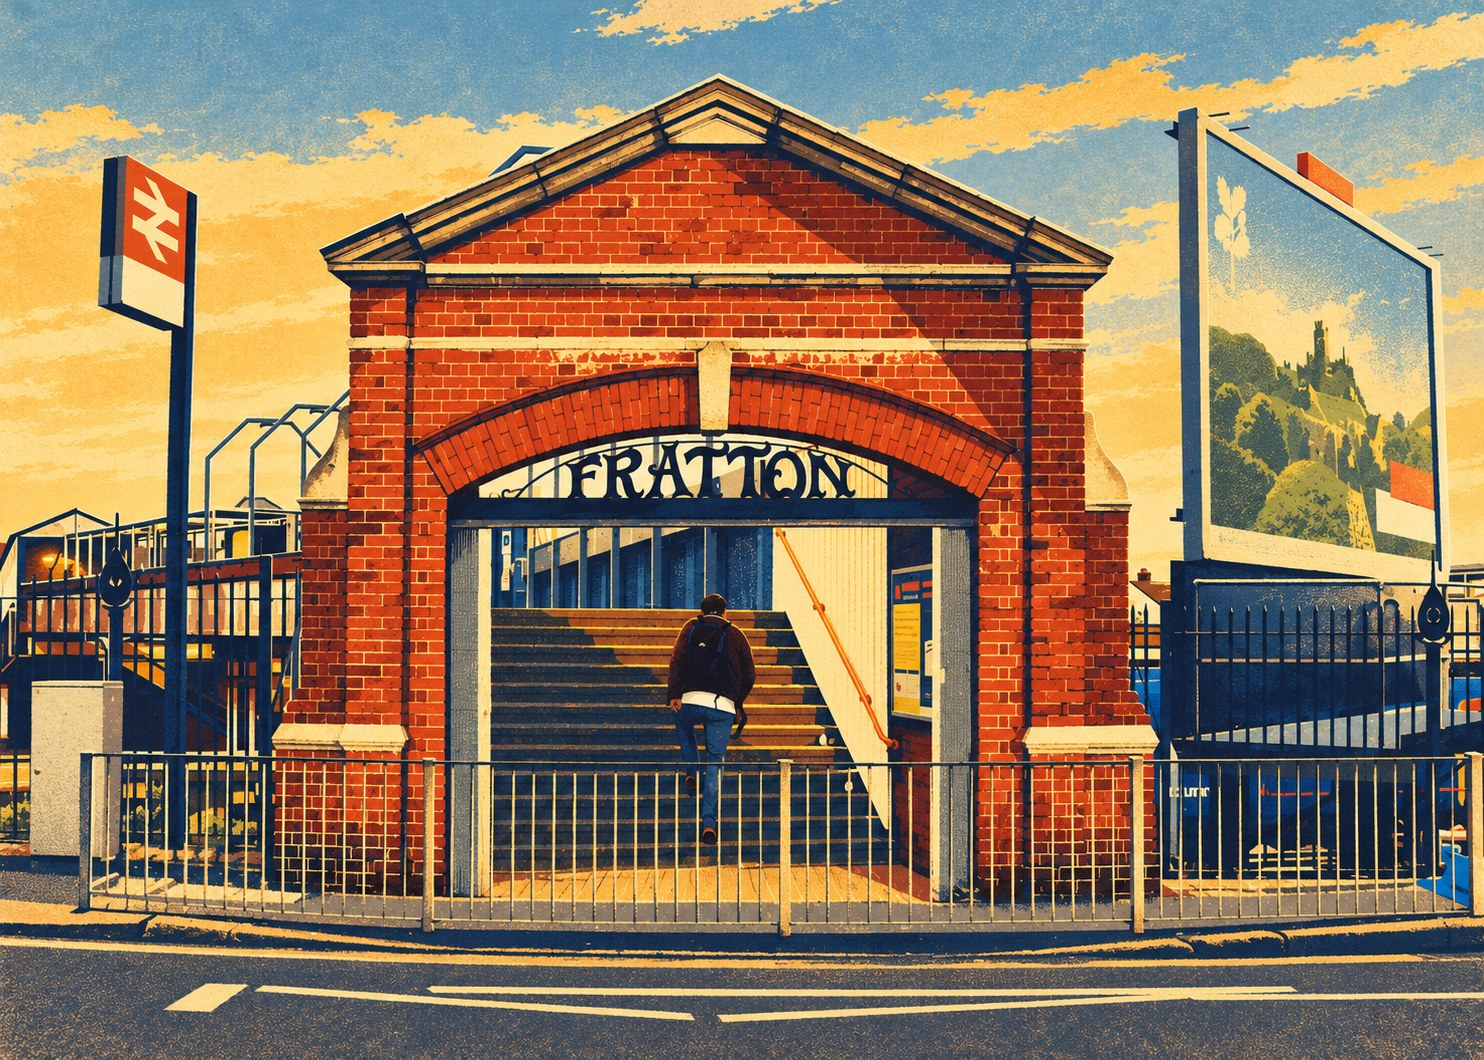
\includegraphics[width=\textwidth]{frattonstation.jpg}\par
\vspace{1.2cm}
{\large Hans A.\ Winther\par}
\vspace{0.3cm}
{\normalsize Institute of Theoretical Astrophysics, University of Oslo\par}
\vfill
{\normalsize \github{HAWinther/FML}\par}
\vspace{0.3cm}
{\small Documentation version of \today\par}
\end{titlepage}

\cleardoublepage
\chapter*{Preface}
\addcontentsline{toc}{chapter}{Preface}

\fml{} is a C++17 library for cosmology and the large-scale structure of the Universe. It started as a collection of
the tools needed for fast approximate simulations (particle--mesh gravity, Lagrangian perturbation theory, the COLA
method and modified-gravity solvers) and has grown into a library that covers the whole chain from the expansion
history and the linear Einstein--Boltzmann equations, through initial conditions and $N$-body, hydrodynamical and
wave dark matter simulations, to halo and void finding, clustering statistics, survey estimators, analytic nonlinear
models and statistical inference.

This book documents all of it. For every feature it gives
\begin{itemize}
\item the equations that are solved, derived to the extent needed to state the conventions unambiguously;
\item the algorithms used to solve them, with the numerical choices that matter for accuracy and cost;
\item how the feature is used from code (the main classes and functions, a short example and the important options);
\item how it is validated, and against which external codes and papers;
\item references to the literature and to the codes the methods come from or are compared with.
\end{itemize}
The module guides in the repository (\file{README.md} files next to the code) remain the authoritative description of
interfaces and test procedures; this book collects the physics and numerics behind them in one place, with a common
notation. \Cref{app:module-index} maps every module directory of the repository to the chapters that describe it.

\paragraph*{How to read this book.} \Cref{part:intro} (\cref{ch:introduction,ch:conventions,ch:getting-started}) gives an overview, shows how to build and run the code and
fixes the conventions (units, Fourier transforms, grids, parallel layout, cosmological notation) used everywhere
else. The remaining parts follow the flow of a typical calculation: the numerical infrastructure, the homogeneous
universe and linear theory, analytic models of nonlinear structure, initial conditions, simulations, structure
identification, clustering statistics, and finally surveys, lensing and inference. Each chapter starts with a summary
of the modules it covers and can be read on its own.

\paragraph*{Status.} The book is written alongside the code and describes the library as of the date under each
chapter title. Facts, defaults and validation numbers are taken from the source, the module documentation and the
tests; where a result is a one-off measurement or an experiment rather than a regression test, the text says so. When
the code changes, the module's own documentation is the authority until the chapter is updated.

\tableofcontents

\mainmatter
% ---------------------------------------------------------------------------------------------------------------------
\part{Introduction}\label{part:intro}
\chapter{Introduction}\label{ch:introduction}
\chapterstatus{written}{2026-11-15}

\section{What FML is}

\fml{} is a library of building blocks, together with a few complete programs built from them. The building blocks
are templated C++ classes and functions in the namespace \nsp{FML}, one directory (\emph{module}) per topic. Most
modules are header-only; the ones with substantial compiled code (the Einstein--Boltzmann solver, recombination,
parts of the cosmology) have their own \file{Makefile}. Almost everything works both serially and in parallel with
MPI and OpenMP, with the same code: the parallel layout (\cref{ch:parallelism}) is part of the data structures, not
of the user code.

The complete programs are
\begin{itemize}
\item \textbf{SimulationCode} (\cref{ch:simulation-code}), a configurable particle--mesh / COLA / P$^3$M simulation code
      with a large library of cosmologies and theories of gravity, multiple particle species, on-the-fly analysis and
      initial conditions from a transfer-function file, from tabulated transfer tables or from the built-in
      Einstein--Boltzmann solver;
\item the \textbf{Einstein--Boltzmann solver} (\cref{ch:background,ch:recombination,ch:linear-perturbations,ch:cmb-spectra,ch:extended-models}),
      a line-of-sight code for the CMB and matter spectra in $\Lambda$CDM and some twenty extended models;
\item \textbf{SnapshotAnalyzer} (\cref{ch:snapshot-analyzer}), a standalone analysis program for simulation snapshots
      from any code;
\item \textbf{CosmologyFitting} (\cref{ch:sampling-fitting}), likelihoods and samplers built on the solver.
\end{itemize}

\section{Design principles}

A few principles recur throughout the library and explain many of the interfaces described in this book.

\paragraph*{One implementation of each physical quantity.} The expansion history, the quasi-static limits of
modified-gravity theories, the growth factors, the halo-model ingredients and the perturbation-theory kernels are each
implemented once and reused: the same \cls{Background} drives the Einstein--Boltzmann solver, the simulation time
stepping, the growth factors, spherical collapse and the halo model; the same \cls{QuasiStaticGravity} gives
$\mu(k,a)$ to the Boltzmann solver, to the LPT growth factors, to the one-loop hybrid bias spectra and to the
simulation code.

\paragraph*{Ownership is explicit.} Distributed data (particles in slabs, grids with local slices) and replicated data
(catalogues that every task holds in full) obey different rules, and each API states which it expects. Collective
functions must be called by all tasks.

\paragraph*{Units are explicit.} Box-unit positions in $[0,1)$ for particles and grids, $\hMpc$ and $\Mpch$ for
large-scale structure, SI or Mpc units in the Boltzmann code; \cref{ch:conventions} lists them and every chapter
states its own.

\paragraph*{Validation is part of a feature.} Every module has regression tests (analytic limits, manufactured
solutions, conservation laws, comparisons with external codes such as CLASS, CAMB, hi\_class, FAST-PT, velocileptors,
ReACT, ROCKSTAR or FINUFFT). The validation boxes in this book summarise them; the scope statements of the module
guides say what a passed test does and does not establish.

\section{Building}

\fml{} needs a C++17 compiler. The optional dependencies are switched on with make variables: \code{USE_MPI},
\code{USE_OMP}, \code{USE_FFTW} (FFTW3, with its MPI build for MPI runs), \code{USE_FFTW_THREADS}, \code{USE_GSL},
\code{USE_LUA} (parameter files), \code{USE_CGAL} (triangulations), \code{USE_HDF5} and \code{USE_PYTHON}. Machine
specific paths go in \file{FML/Makefile.local}; the shared rules are in \file{FML/Makefile.config}.
\begin{paramfile}[Makefile.local]
CXX_SERIAL   = c++
CXX_MPI      = mpicxx
LOCAL_PREFIX = /opt/homebrew      # where FFTW, GSL, Lua, ... are installed
\end{paramfile}
The test suite is built and run with \code{make -C FML test} (optionally with \code{MPIRUN=mpirun NP_LIST="1 2 4"}),
the examples with \code{make -C FML examples}, the simulation code with \code{make -C FML/SimulationCode} (or its CMake
build) and the Einstein--Boltzmann solver with \code{make} in \file{Cosmology/EinsteinBoltzmannSolver}. The file
\file{FML/BUILDING.md} is the reference for all build options.

\section{Map of the library}

\Cref{tab:module-map} groups the modules by the parts of this book. The full mapping of directories to sections is in
\cref{app:module-index}.

\begin{table}[htbp]
\centering\small
\caption{The modules of \fml{} grouped by the parts of this book.}\label{tab:module-map}
\begin{tabularx}{\textwidth}{@{}lX@{}}
\toprule
Part & Modules \\
\midrule
Infrastructure & \file{Global}, \file{PencilDomain}, \file{PeanoHilbertDomain}, \file{FFTWGrid}, \file{MPIGrid},
  \file{AdaptiveMPIGrid}, \file{MPIParticles}, \file{ParticleTypes}, \file{ParticlesInBoxes}, \file{KDTree},
  \file{Interpolation}, \file{Smoothing}, \file{NUFFT}, \file{Math}, \file{ODESolver}, \file{Spline}, \file{FFTLog},
  \file{RandomGenerator}, \file{LatinHyperCube}, \file{MultigridSolver}, \file{GadgetUtils}, \file{RamsesUtils},
  \file{FileUtils}, \file{ParameterMap}, \file{LuaFileParser}, \file{Units}, \file{Timing}, \file{MemoryLogging},
  \file{Performance}, \file{Plotting}, \file{Visualization}, \file{Chunkpix}, \file{ExampleData},
  \file{MakePythonWrapper}, \file{PythonAnalysis} \\
Linear theory & \file{Cosmology/Background}, \file{Cosmology/Recombination}, \file{Cosmology/Perturbations},
  \file{Cosmology/Spectra}, \file{Cosmology/EinsteinBoltzmannSolver}, \file{Cosmology/Growth},
  \file{TransferProviders}, \file{InitialConditions} \\
Nonlinear models & \file{PerturbationTheory}, \file{SphericalCollapse}, \file{HaloModel}, \file{AxionHMcode},
  \file{Emulator} \\
Initial conditions & \file{RandomFields}, \file{LPT}, \file{GlassIC} \\
Simulations & \file{NBody}, \file{ShortRangeGravity}, \file{SimulationCode}, \file{AMRCode}, \file{Hydrodynamics}, \file{SPH},
  \file{WaveDarkMatter}, \file{PGD}, \file{Baryonification} \\
Structures & \file{FriendsOfFriends}, \file{PhaseSpaceHaloFinder}, \file{HaloHistory}, \file{CosmicWeb},
  \file{TidalTensor}, \file{Morphology}, \file{VoidFinders}, \file{Triangulation} \\
Statistics & \file{ComputePowerSpectra}, \file{PairCounting}, \file{ThreePointCorrelation}, \file{CountsInCells},
  \file{Environment}, \file{ConnectedFourPoint}, \file{EnsembleStatistics}, \file{HOD} \\
Surveys and inference & \file{Survey}, \file{WeakLensing}, \file{FieldLevel}, \file{MCMC}, \file{CosmologyFitting} \\
Applications & \file{Analysis}, \file{SnapshotAnalyzer} \\
\bottomrule
\end{tabularx}
\end{table}

\chapter{Conventions and notation}\label{ch:conventions}
\chapterstatus{written}{2026-11-14}

This chapter fixes the conventions used throughout the library and the book. Where a module deviates (for example
the Einstein--Boltzmann solver, which works internally in SI units), the chapter on that module says so.

\section{Units}

\begin{itemize}
\item \textbf{Simulation and grid units.} Particle positions and grid coordinates are in units of the box size,
      $\vx\in[0,1)^N$ (a position equal to $1$ is allowed and wraps to $0$). A grid has $N_{\rm mesh}$ cells per
      dimension, cell size $1/N_{\rm mesh}$, and the cell with integer coordinates $\bm i$ has its corner at
      $\bm i/N_{\rm mesh}$ (cell-centred quantities are at $(\bm i+\tfrac12)/N_{\rm mesh}$ only where stated).
      Physical lengths are recovered by multiplying with the box size $B$, usually in $\Mpch$.
\item \textbf{Large-scale structure.} Lengths in $\Mpch$, wavenumbers in $\hMpc$, power spectra in $(\Mpch)^3$,
      masses in $h^{-1}M_\odot$, velocities in km/s unless stated.
\item \textbf{Cosmology.} $H_0=100h$\,km\,s$^{-1}$\,Mpc$^{-1}$; $E(a)=H(a)/H_0$; density parameters
      $\Om_i=\rho_i/\rho_{c}$ with $\rho_c=3H^2/(8\pi G)$; today's critical density $\rho_{c0}=3H_0^2/(8\pi G)$.
      The \code{Background} module (\cref{ch:background}) uses $E$ dimensionless, conformal time and distances in
      $\Mpch$ and cosmic time in Gyr; the Einstein--Boltzmann solver uses SI units internally and Mpc$^{-1}$ for $k$
      in its parameter files.
\item \textbf{Constants.} All physical constants come from \file{Units/Units.h}: \nsp{FML::UTILS::SI} holds
      compile-time SI values (the cosmology code aliases it as \nsp{FML::COSMOLOGY::Constants}), and
      \cls{ConstantsAndUnits} gives them in another unit system (SI, Planck, ParticlePhysics, Cosmology or
      user-defined). Energies such as the hydrogen binding energy \code{epsilon_0} are stored in joules.
\end{itemize}

\section{Time variables}

The library uses several time variables, always with the same symbols:
\begin{center}\small
\begin{tabular}{@{}lll@{}}
\toprule
Symbol & Definition & Used in \\
\midrule
$a$, $z$ & scale factor ($a_0=1$) and redshift $1+z=1/a$ & everywhere \\
$x$ & $x=\ln a$ & background, Boltzmann code, growth factors \\
$t$ & cosmic time, $\dd t=\dd x/H$ & ages, time stepping \\
$\eta$ & conformal time, $c\,\dd t=a\,\dd\eta$ & line of sight, Boltzmann code \\
$\chi$ & comoving distance, $\chi=c(\eta_0-\eta)$ & distances, lightcones, lensing \\
$\Hp$ & conformal Hubble rate $\Hp=aH$ & perturbations \\
\bottomrule
\end{tabular}
\end{center}
A prime denotes $\dd/\dd x$ unless stated otherwise (in a few places, clearly marked, it is $\dd/\dd\eta$); a dot
denotes $\dd/\dd t$.

\section{Fourier transforms}

\paragraph*{Continuous.} For a field in a periodic box of side $B$ (or in infinite space),
\begin{equation}
\delta(\vk)=\int\dd^3x\,\delta(\vx)\,e^{-i\vk\cdot\vx},\qquad
\delta(\vx)=\int\frac{\dd^3k}{(2\pi)^3}\,\delta(\vk)\,e^{i\vk\cdot\vx},
\end{equation}
and the power spectrum is defined by
$\langle\delta(\vk)\delta^*(\vk')\rangle=(2\pi)^3\delta_D(\vk-\vk')P(k)$. The dimensionless power spectrum is
$\Delta^2(k)=k^3P(k)/(2\pi^2)$. For the primordial curvature perturbation $\mathcal{R}$ we write
$\mathcal{P}_\mathcal{R}(k)=k^3P_\mathcal{R}(k)/(2\pi^2)=A_s(k/k_{\rm pivot})^{n_s-1+\frac12\alpha_s\ln(k/k_{\rm pivot})}$.

\paragraph*{Discrete.} \cls{FFTWGrid} uses the sign convention of FFTW, forward transforms with $e^{-i\vk\cdot\vx}$,
and normalises the \emph{forward} transform,
\begin{equation}
\delta_{\bm n}=\frac{1}{N_{\rm mesh}^N}\sum_{\bm i}\delta_{\bm i}\,e^{-2\pi i\,\bm n\cdot\bm i/N_{\rm mesh}},\qquad
\delta_{\bm i}=\sum_{\bm n}\delta_{\bm n}\,e^{2\pi i\,\bm n\cdot\bm i/N_{\rm mesh}},
\end{equation}
so that the Fourier coefficients are the dimensionless amplitudes of the modes and a constant field has
$\delta_{\bm 0}$ equal to its mean. The wave vector of mode $\bm n$ (with $n_j\in(-N_{\rm mesh}/2,N_{\rm mesh}/2]$) is
$\vk=2\pi\bm n$ in box units, i.e.\ $\vk=2\pi\bm n/B$ physically. With this normalisation the power spectrum
estimated from a grid is $P(k)=B^3\langle|\delta_{\bm n}|^2\rangle$ averaged over a shell
(\cref{ch:power-spectra}). Real-to-complex transforms store the half space $n_N\ge0$ of the last dimension; modes with
$n_N=0$ or $n_N=N_{\rm mesh}/2$ appear once but represent two complex-conjugate modes, which the binning routines take
into account.

\section{Parallel layout}

With MPI, all communication goes through \code{FML::communicator} (normally \code{MPI_COMM_WORLD}). The task index is
\code{FML::ThisTask} and the number of tasks \code{FML::NTasks}. The default decomposition is in \emph{slabs} along the
first coordinate: task $t$ owns $x\in[x_{\min}^{(t)},x_{\max}^{(t)})$ (\code{FML::xmin_domain},
\code{FML::xmax_domain}) for its particles, and the corresponding slices of every grid. Grids can allocate extra
slices on the left and right (\emph{ghost} slices) that are filled from the neighbours when needed. Pencil and
Peano--Hilbert decompositions exist as separate modules (\cref{ch:parallelism}). OpenMP is used inside a task.

\section{Cosmological notation}

\begin{center}\small
\begin{tabularx}{\textwidth}{@{}lX@{}}
\toprule
Symbol & Meaning \\
\midrule
$\Om_b,\Om_{\rm cdm},\Om_\gamma,\Om_\nu,\Om_k,\Om_\Lambda$ & density parameters today (baryons, CDM, photons,
  massless neutrinos, curvature, cosmological constant) \\
$\Om_m$ & total matter today: $\Om_b+\Om_{\rm cdm}+\Om_{\nu,\rm massive}$ \\
$\omega_i$ & physical densities $\Om_ih^2$ \\
$K$ & spatial curvature $K=-\Om_k(H_0/c)^2$ ($K>0$ closed) \\
$\delta_i,\,\theta_i,\,v_i$ & density contrast, velocity divergence, velocity potential of species $i$ \\
$\Phi,\Psi$ & metric potentials of the conformal Newtonian gauge (\cref{ch:linear-perturbations} for the sign
  conventions) \\
$D_1,D_2,\dots$; $f=\dd\ln D/\dd\ln a$ & LPT growth factors and growth rate \\
$\mu(k,a),\Sigma(k,a)$ & modification of the Poisson and lensing equations \\
$\sigma_R$, $\sigma_8$ & rms linear density in top-hat spheres of radius $R$ ($8\Mpch$) \\
\bottomrule
\end{tabularx}
\end{center}

\section{Notation in this book}

Class and function names are set in \code{typewriter}, and parameters of the programs (parameter files of the
Boltzmann solver and of SimulationCode) also in \code{typewriter}; both are listed in the index. File paths are
relative to the \file{FML/} directory of the repository. Each chapter starts with a module box listing the headers and
documentation files that implement and describe what the chapter covers, and \emph{implementation} and
\emph{validation} boxes summarise the numerical methods and the tests.

\chapter{Getting started}\label{ch:getting-started}
\chapterstatus{written}{2026-11-14}

How to configure and build \fml{}, write and compile a first program, run the tests, and use the four programs that come with the
library. \file{FML/BUILDING.md} is the reference for all build options and \file{FML/CAPABILITIES.md} lists the modules with their
scope and examples.

\begin{modulebox}{Build system}
\file{Makefile.config} (compilers, feature flags, dependency paths, rules), \file{Makefile.local} (machine-specific settings, not under
version control), the module and example \file{Makefile}s, \file{SimulationCode/CMakeLists.txt}; \file{tests/TestHelpers.h} for tests.\par
Documentation: \file{BUILDING.md}, \file{CAPABILITIES.md}.
\end{modulebox}

\section{Requirements and configuration}\label{sec:gs-config}

\fml{} needs a C++17 compiler. Everything else is optional and switched on per build:

\begin{center}\small
\begin{tabularx}{\textwidth}{@{}lX@{}}
\toprule
Make variable & Enables \\
\midrule
\code{USE_MPI=true} & MPI (\code{mpicxx}); all communication through \code{FML::communicator} \\
\code{USE_OMP=true} & OpenMP loops (\code{OMP_NUM_THREADS}) \\
\code{USE_FFTW=true} & FFTW grids and transforms (with MPI an MPI-enabled FFTW) \\
\code{USE_FFTW_THREADS=true} & threaded FFTs (the FFTW threads library; separate from OpenMP loops) \\
\code{USE_GSL=true} & GSL splines, ODEs and quadrature (the cosmology code needs it) \\
\code{USE_LUA=true} & Lua parameter files (\file{SimulationCode}, \file{SnapshotAnalyzer}) \\
\code{USE_CGAL=true} & Delaunay tessellations (DTFE, ZOBOV, ORIGAMI halos) \\
\code{USE_HDF5=true} & GADGET HDF5 snapshots and HDF5 catalogues \\
\code{USE_PYTHON=true} & Python embedding for plotting and the SWIG wrappers \\
\code{USE_MEMORYLOG=true}, \code{USE_DEBUG=true}, \code{USE_SANITIZER=true} & memory logging, debug checks, address sanitizer \\
\bottomrule
\end{tabularx}
\end{center}

Machine-specific settings (compilers and dependency paths) go in \file{FML/Makefile.local}; variables on the command line take precedence:

\begin{paramfile}[Makefile.local]
CXX_SERIAL   = c++
CXX_MPI      = mpicxx
LOCAL_PREFIX = /path/to/dependencies    # or FFTW_INCLUDE, FFTW_LIB, GSL_INCLUDE, ...
\end{paramfile}

Object files do not record the flags they were built with: clean (\code{make clean}) before switching between serial and MPI, precision
or compilers, or use separate build directories. Single and long-double FFT precision (\code{SINGLE_PRECISION_FFTW},
\code{LONG_DOUBLE_PRECISION_FFTW}) need the matching FFTW libraries (e.g.\ \code{FFTW_LINK=-lfftw3f}).

\section{A first program}\label{sec:gs-first}

Include the directory that \emph{contains} \file{FML}, and link \file{FML/Global/Global.cpp} (plus the implementation files of the modules used,
e.g.\ \file{Spline.cpp}, \file{ODESolver.cpp}, \file{FFTLog.cpp}; the Makefile of a related example lists them). The runtime sets up MPI, FFTW and
OpenMP automatically (\cref{sec:par-runtime}).

\begin{cppcode}[particles.cpp: particles on a lattice and their power spectrum]
#include <FML/MPIParticles/MPIParticles.h>
#include <FML/ComputePowerSpectra/ComputePowerSpectrum.h>
struct Particle {
    double pos[3]{};
    double * get_pos() { return pos; }
    constexpr int get_ndim() const { return 3; }
};
int main() {
    FML::PARTICLE::MPIParticles<Particle> part;
    part.create_particle_grid(64, 1.5);                      // 64^3 particles in [0,1)^3
    FML::CORRELATIONFUNCTIONS::PowerSpectrumBinning<3> pofk(32);
    FML::CORRELATIONFUNCTIONS::compute_power_spectrum<3>(
        64, part.get_particles_ptr(), part.get_npart(), part.get_npart_total(), pofk, "CIC", false);
    if (FML::ThisTask == 0) pofk.info();
}
\end{cppcode}

\begin{paramfile}[Compiling and running]
# serial, from the folder containing FML
c++ -std=c++17 -O3 -I. -DUSE_FFTW particles.cpp FML/Global/Global.cpp -lfftw3 -o particles
# MPI + OpenMP
mpicxx -std=c++17 -O3 -fopenmp -I. -DUSE_MPI -DUSE_OMP -DUSE_FFTW -DUSE_FFTW_THREADS \
       particles.cpp FML/Global/Global.cpp -lfftw3_mpi -lfftw3_threads -lfftw3 -o particles
OMP_NUM_THREADS=4 mpirun -np 2 ./particles
\end{paramfile}

Every module has an \file{example/} folder with a Makefile that uses the shared configuration (\code{make -C FML examples}). The examples need
no data files: those that read particles, a survey or a snapshot make a small synthetic data set with
\file{ExampleData/ExampleData.h}.

\section{Tests}\label{sec:gs-tests}

The regression tests are in \file{FML/tests} and in the \file{tests/} folders of the modules, with references from other codes stored as fixtures:

\begin{paramfile}[Running the tests]
make -C FML test MPIRUN=mpirun NP_LIST="1 2 4"     # the standard suite on 1, 2 and 4 tasks
make -C FML/tests test_core USE_MPI=false USE_FFTW=false USE_GSL=false   # dependency-free core
make -C FML/Cosmology/EinsteinBoltzmannSolver test # the Einstein-Boltzmann solver
make -C FML/CountsInCells/tests run USE_MPI=false  # one module
\end{paramfile}

Tests use \file{tests/TestHelpers.h}: \code{check} is collective (it fails on every task if it fails on any), \code{check_local} is not, and
\code{summary} sets the exit code. The validation boxes in this book cite the test files.

\section{The programs}\label{sec:gs-programs}

\begin{itemize}
\item \file{Cosmology/EinsteinBoltzmannSolver/cmb}: background, recombination, perturbations, CMB and matter spectra, nonlinear spectra
      (\cref{ch:background,ch:recombination,ch:linear-perturbations,ch:cmb-spectra}): \code{./cmb params/planck2018.ini}, parameters on the
      command line override the file, \code{./cmb --write-defaults my.ini} writes every parameter with its default.
\item \file{SimulationCode/nbody}: PM/COLA/TreePM simulations with modified gravity, neutrinos, gas and on-the-fly analysis
      (\cref{ch:simulation-code}): \code{mpirun -np 4 ./nbody parameterfile.lua}; \code{./nbody --parameters PARAMETERS.md} writes the parameter reference.
      Also a CMake build.
\item \file{SnapshotAnalyzer}: the same analyses on GADGET snapshots of any code (\cref{ch:snapshot-analyzer}).
\item \file{CosmologyFitting/mcmc}: MCMC and best fits to supernova, BAO and CMB data (\cref{ch:sampling-fitting}).
\end{itemize}
The parameter files of all four reject unknown or mistyped parameters. Python users can install the catalogue-statistics package with
\code{python -m pip install ./FML/PythonAnalysis} (\cref{sec:io-python}).

\section{Where to go next}\label{sec:gs-next}

\Cref{ch:conventions} fixes the units and conventions used throughout. For a given task: initial conditions, \cref{ch:random-fields,ch:lpt};
running a simulation, \cref{ch:nbody-pm,ch:simulation-code}; analysing one, \cref{ch:power-spectra,ch:halo-finding,ch:snapshot-analyzer}; linear
theory and fitting, \cref{ch:background,ch:sampling-fitting}; the analytic nonlinear models, \cref{ch:perturbation-theory,ch:halo-model}. The module
index (\cref{app:module-index}) maps every folder to its chapters.


\part{Infrastructure}
\chapter{Parallelism and domain decomposition}\label{ch:parallelism}
\chapterstatus{written}{2026-11-14}

\fml{} is written for distributed memory with MPI and shared memory with OpenMP, and every module also compiles and
runs without either. This chapter describes the runtime that sets them up, how the box is decomposed over the tasks
(slabs by default, pencils and Peano--Hilbert ranges as alternatives) and the communication helpers that the modules
share.

\begin{modulebox}{Global}
\nsp{FML}: \file{Global/Global.h} (runtime, reductions, \code{assert_mpi}), \file{Global/Domain.h} (\cls{Domain},
\cls{SlabDomain}, \cls{PencilDomain}, \cls{PeanoHilbertDomain}), \file{Global/DomainBuffer.h} (\cls{DomainBuffer}),
\file{Global/PeriodicSlabExchange.h}, \file{Global/ChunkedExchange.h}, \file{Global/MPICounts.h},
\file{Global/SystemMemory.h}.\par
Documentation: \file{Global/MPICounts.md}. Tests: \file{tests/test_domain.cpp}, \file{tests/test_mpi_counts.cpp}.
\end{modulebox}
\begin{modulebox}{PencilDomain, PeanoHilbertDomain}
\nsp{FML::GRID}: \file{PencilDomain/PencilGrid.h} (\cls{PencilGrid}), \file{PencilDomain/CPencilGrid.h}
(\cls{CPencilGrid}).
\nsp{FML::DOMAIN_DECOMPOSITION::PEANO_HILBERT}: \file{PeanoHilbertDomain/HilbertCurve.h} (\cls{HilbertCurve}),
\file{PeanoHilbertDomain/DistributedGrid3D.h} (\cls{DistributedGrid3D}).\par
Documentation: \file{PencilDomain/README.md}, \file{PeanoHilbertDomain/README.md}. Tests: \file{PencilDomain/tests},
\file{PeanoHilbertDomain/tests} and the \file{tests/test_*_pencil.cpp} suite.
\end{modulebox}

\section{The runtime}\label{sec:par-runtime}

With the compile flags \code{USE_MPI}, \code{USE_OMP} and \code{USE_FFTW} the library sets itself up automatically: a
singleton constructed at program start initialises MPI (with thread support), FFTW (with its MPI and threads interfaces)
and the globals, and finalises them at exit. With \code{NO_AUTO_FML_SETUP} the user calls \code{MPI_Init}, may set
\code{FML::communicator} to a sub-communicator (all communication of the library goes through it; default
\code{MPI_COMM_WORLD}) and then calls \code{FML::init_fml()} (and \code{FML::GRID::init_fftw}).

The globals are \code{FML::ThisTask} and \code{FML::NTasks}, the number of threads, whether MPI and threads can be combined
with FFTW, the local x-range of the particle domain \code{xmin_domain}, \code{xmax_domain} and the domain itself
(\cref{sec:par-domains}). On Linux the CPU affinity masks are checked: \code{NTasksThreadsShareCores} counts the tasks
that have fewer cores than OpenMP threads, a common misconfiguration of \code{mpirun}.

\paragraph*{Collectives and errors.} Inplace reductions of one value or an array (\code{SumOverTasks}, \code{MinOverTasks},
\code{MaxOverTasks}, \code{SumArrayOverTasks}, \ldots; arithmetic types reduce with \code{MPI_Allreduce} in bounded
chunks, others are gathered and reduced locally) and gathers (\code{GatherFromTasks}). Errors go through
\code{assert_mpi(condition, message)}, which prints the message and calls \code{MPI_Abort} rather than \code{abort} so that
the other tasks do not deadlock. Many modules can instead throw (e.g.\ \code{SPLINE_THROW_ON_ERROR},
\code{ODESOLVER_THROW_ON_ERROR}) so that a caller such as an MCMC can recover. With \code{MEMORY_LOGGING} every large
allocation of the standard containers is logged (\cref{ch:io-utilities}).

\paragraph*{Threads.} Grid loops are parallelised over \emph{rows} (lines of cells along the last axis) rather than slices,
because a task can have fewer slices than threads but not fewer rows. Particle loops use OpenMP with atomic or coloured
updates where they write to shared grids (\cref{ch:mass-assignment}).

\section{Domains}\label{sec:par-domains}

The unit box $[0,1)^D$ is decomposed by a \cls{Domain}, a \code{std::variant} of three types whose ownership queries
(\code{owner(pos)}, \code{owner_near(task, pos)}, \code{contains(task, pos)}) are inline switches without virtual calls:
\begin{itemize}
\item \cls{SlabDomain}: task $i$ owns $x\in[x_{\min,i},x_{\max,i})$, the ranges partitioning $[0,1)$ in rank order (empty
      slabs allowed). The default, given by \code{xmin_domain} and \code{xmax_domain} of each task (equal slabs
      $[i/N_{\rm tasks},(i+1)/N_{\rm tasks})$ from \code{init_fml}). Grids, particles and nearly all algorithms support it.
      \code{owner} binary-searches the edges; \code{owner_near} checks the neighbours first, where most leaving particles go.
\item \cls{PencilDomain}: a $P_0\times P_1$ process grid in $(x,y)$; the task with coordinates $(i_x,i_y)$ is rank
      $i_xP_1+i_y$ and owns a box in $x$ and $y$ and all of $z$. The decomposition of \cls{PencilGrid}.
\item \cls{PeanoHilbertDomain} (3D): contiguous ranges of the Peano--Hilbert key, built load-balanced from the particles.
\end{itemize}
The global instance \code{FML::domain} is set with \code{FML::set_domain} (collectively); \cls{MPIParticles} takes it when
created, so particles live on the task of their grid cells (\cref{ch:particles}). Code that needs slabs asserts it
(\code{require_slab}).

\paragraph*{Slabs.} A slab grid and the particles share the x-ranges; each task stores extra slices to the left and right
(ghosts) for the stencils of mass assignment, interpolation and finite differences. FFTW-MPI's slab transforms require
$N_{\rm mesh}$ divisible by the number of tasks and can use at most $N_{\rm mesh}$ tasks (one slice each).

\paragraph*{Pencils.} \cls{PencilGrid} splits two axes, so up to $N_{\rm mesh}^2$ tasks can be used and any $N_{\rm mesh}$ works
(the process grid from \code{MPI_Dims_create}, the edges on cells as evenly as possible). In 3D the transform is r2c along
$z$, a transpose within the row of tasks and an FFT along $y$, a transpose within the column and an FFT along $x$ (FFTW's
guru interface; the transposes pack cache-blocked blocks and exchange them with \code{MPI_Alltoallv}). In Fourier space a
task has all $k_x$ and parts of $k_y$ and $k_z$. On 2 tasks the forward and inverse FFTs take 0.9--1.3 times the slab time
and a whole N-body run 1.05--1.2 times; pencils pay off when the number of tasks approaches $N_{\rm mesh}$ or does not divide
it. The library, \file{SimulationCode} and the snapshot analyser are written against a common grid interface
(\cref{sec:grids-interface}) and run on slabs or pencils:

\begin{cppcode}[A run on pencils]
FML::set_domain(FML::pencil_domain());          // or pencil_domain(px, py)
auto grid = FML::GRID::make_grid<FML::GRID::PencilGrid<3>>(Nmesh, n_left, n_right);
FML::PARTICLE::MPIParticles<Particle> part;     // takes FML::domain
\end{cppcode}

\paragraph*{Peano--Hilbert ranges.} \cls{HilbertCurve} maps integer coordinates to 64-bit Hilbert keys with Skilling's
transpose algorithm \cite{Skilling2004} ($D=2$--6; in 3D up to 21 bits per coordinate). It is the one key implementation
of the library, used by \cls{AdaptiveMPIGrid} (\cref{sec:mg-amr}) and the particle domain. \code{PeanoHilbertDomain::build}
reduces a distributed prefix histogram of the keys ($2^{b_h}$ counters, $b_h\le20$) and cuts it into approximately
equal-particle contiguous key ranges at bin edges; identical keys always have the same owner, and empty ranges are allowed.
\cls{DistributedGrid3D} stores the cells of each task's key range in key order (not a rectangular block) with halo lists for
face or full cube stencils and collective remote reads. This decomposition is not yet used by \file{SimulationCode}.

\section{Communication patterns}\label{sec:par-communication}

\begin{itemize}
\item \emph{Ghost slices} of grids: \code{communicate_boundaries} sends the edge slices to the neighbours (forwarded from
      tasks further away when there are more ghost slices than local slices); \code{add_contribution_from_extra_cells}
      adds the ghosts back after mass assignment. \cls{GhostedCells} gives the same for per-cell data of any type
      (\cref{sec:grids-mpigrid}).
\item \emph{Particle migration} (\cref{ch:particles}): to the owner of the new position, with wide counters and bounded
      message sizes.
\item \emph{Buffer exchanges}: \cls{DomainBuffer} sends copies of the particles within a distance of a task's box to the
      neighbours (2 for slabs, up to 8 for pencils, corners included), optionally shifted across the periodic box, and maps
      values forward to the copies and back to the originals. It is used by the friends-of-friends, Delaunay and other particle
      methods. \code{append_periodic_slab_ghosts} (and \code{append_periodic_domain_ghosts} for pencils) does the same for records, skipping peers whose box is beyond the buffer.
\item \emph{Chunked exchange}: \code{exchange_records_chunked} delivers records to their destination task without a flattened send
      buffer or a full receive buffer, in rounds of at most 8\,MiB by default, with all tasks executing the same number of
      rounds.
\end{itemize}

\paragraph*{MPI counts.} MPI counts and displacements are \code{int}, so transfers above $2^{31}$ elements or bytes overflow
silently in naive code. \file{MPICounts.h} provides checked addition and multiplication, layouts that are verified before
any payload is sent (throwing \code{std::overflow_error} collectively), and gathers of fixed-size records. Particle
migration exchanges its counters as \code{unsigned long long} and chunks the payload by a message cap (default
\code{INT_MAX}); the other exchanges (sheets, FoF, ORIGAMI, Delaunay, void catalogues, MCMC summaries, \ldots) were audited
for the same limits (\file{MPICounts.md}).

\paragraph*{Memory.} \file{SystemMemory.h} reads the resident set size and its peak per task and prints their range over
tasks; the allocation log of \code{MEMORY_LOGGING} is described in \cref{ch:io-utilities}.

\begin{validation}[Validation: domains and communication]
\file{tests/test_domain.cpp} on 1, 2 and 4 tasks: the global Slab and its ranges; \code{owner} and \code{owner_near} of
slabs (with empty slabs), pencils and Peano--Hilbert ranges against brute force; \cls{MPIParticles} on every domain type
(\code{communicate_particles}, distributed and replicated input, checkpoints). \file{tests/test_mpi_counts.cpp}: exact
\code{INT_MAX} boundaries, overflow of aggregate layouts, one-rank failures handled collectively, empty ranks and a real
64-bit count exchange above \code{INT_MAX}. The pencil suite (\file{tests/test_*_pencil.cpp}) checks that the grid-based
modules (assignment, interpolation, LPT, spectra, cosmic web, voids, SPH, multigrid, \ldots) give the same results on slabs
and pencils.
\end{validation}

\chapter{Grids and Fourier transforms}\label{ch:grids-fft}
\chapterstatus{written}{2026-11-14}

Fields are stored on distributed grids with in-place FFTW transforms \cite{Frigo2005}: real grids with real-to-complex
transforms for densities and potentials, complex grids for wave functions and the NUFFT, and generic MPI grids of any type
for the multigrid solvers. Generic algorithms are written against one interface, so they run on slabs and on pencils.

\begin{modulebox}{FFTWGrid}
\nsp{FML::GRID}: \file{FFTWGrid/FFTWGrid.h} (\cls{FFTWGrid}), \file{FFTWGrid/CFFTWGrid.h} (\cls{CFFTWGrid}),
\file{FFTWGrid/FFTWGlobal.h} (precision), \file{FFTWGrid/GridInterface.h}, \file{FFTWGrid/GhostedCells.h}
(\cls{GhostedCells}), \file{FFTWGrid/FourierResampling.h} (\code{resize_fourier_grid}, \cls{FourierResamplingPlan}),
\file{FFTWGrid/CopyFourierModes.h}.\par
Documentation: \file{FFTWGrid/FourierResampling.md}. Tests: \file{tests/test_grids.cpp}, \file{tests/test_complex_grids.cpp},
\file{tests/test_grid_generic.cpp}, \file{tests/test_ghosted_cells.cpp}, \file{tests/test_fourier_resampling.cpp}.
\end{modulebox}
\begin{modulebox}{MPIGrid}
\nsp{FML::GRID}: \file{MPIGrid/MPIGrid.h} (\cls{MPIGrid}), \file{MPIGrid/MPIMultiGrid.h} (\cls{MPIMultiGrid}),
\file{MPIGrid/ConvertMPIGridFFTWGrid.h}. The adaptive grid \cls{AdaptiveMPIGrid} is described with its solver in
\cref{sec:mg-amr}.
\end{modulebox}

\section{FFTWGrid}\label{sec:grids-fftwgrid}

\cls{FFTWGrid} holds an $N_{\rm mesh}^D$ real field ($D\ge2$) split in x-slabs, with the real and the Fourier grid in the
same array: the transforms are in place. The real grid is padded to $2(N_{\rm mesh}/2+1)$ along the last axis; the Fourier
grid has $N_{\rm mesh}^{D-1}(N_{\rm mesh}/2+1)$ complex cells, local in $k_x$. The memory is
\[
[\text{extra slices left}]\;[\text{main grid}]\;[\text{extra slices right}],
\]
so a cell $k$ slices to the left is at \code{index - k * stride_x}, also into the extra slices. The grid records whether it
holds real or Fourier data.

\paragraph*{Conventions.} \code{fftw_r2c()} divides by $N_{\rm mesh}^D$, so the Fourier values are the amplitudes of the
discrete Fourier series, $\delta(\bm x)=\sum_{\bm k}\delta_{\bm k}e^{i\bm k\cdot\bm x}$, and \code{fftw_c2r()} does not
normalise (\cref{ch:conventions}). Wave-vectors are $\bm k=2\pi\bm n$ in box units (multiply by $1/B$ for physical units),
with $n_i\in(-N/2,N/2]$ and $n_D\in[0,N/2]$. A mode with $0<n_D<N/2$ also stands for $-\bm k$ (weight 2 in sums over the
grid; \code{fourier_mode_multiplicity}). The DC mode lives on the task whose slab starts at $x=0$ (\code{has_dc_mode}).
The precision is double by default, float with \code{SINGLE_PRECISION_FFTW} and long double with
\code{LONG_DOUBLE_PRECISION_FFTW}.

\paragraph*{Access.} By local integer coordinates or by index (\code{get_real}, \code{set_real}, \code{add_real},
\code{get_fourier}, \ldots, with \code{_from_index} variants), positions in $[0,1)^D$ (\code{get_real_position}),
wave-vectors and their norms by index, filling from a function of position or wave-vector, and range iterators over the real
or Fourier cells, optionally restricted to rows for OpenMP:

\begin{cppcode}[Filtering a field in Fourier space]
#include <FML/FFTWGrid/FFTWGrid.h>
FML::GRID::FFTWGrid<3> grid(Nmesh, 1, 1);            // one extra slice on each side
grid.fill_real_grid([](std::array<double, 3> & x) { return f(x); });
grid.fftw_r2c();                                     // normalised by 1 / Nmesh^3
#pragma omp parallel for
for (IndexIntType irow = 0; irow < grid.get_local_nrows(); irow++)
    for (auto && i : grid.get_fourier_range_of_rows(irow, irow + 1)) {
        std::array<double, 3> kvec;  double kmag;
        grid.get_fourier_wavevector_and_norm_by_index(i, kvec, kmag);
        grid.set_fourier_from_index(i, grid.get_fourier_from_index(i) * W(kmag / Boxsize));
    }
grid.fftw_c2r();
grid.communicate_boundaries();                       // fill the extra slices
\end{cppcode}

\paragraph*{Plans and wisdom.} FFTW plans are cached and reused by every grid with the same dimension, size, alignment, thread
count and planner flag. The flag is \code{FFTW_ESTIMATE} by default; \code{set_fftw_planner_flag} (or the name
\code{estimate}, \code{measure}, \code{patient}, \code{exhaustive}) selects slower planning for faster transforms, with the grid
data preserved during planning. \code{save_fftw_wisdom} and \code{load_fftw_wisdom} store the plans so that a later run does not
measure again (valid for the same FFTW version, precision, machine and threads; collective, with task 0 doing the file I/O). The
cells of the right extra slices that FFTW may use as scratch space in an in-place transform are backed up and restored.

\paragraph*{Checkpoints and memory.} \code{dump_to_file} and \code{load_from_file} write a raw copy per task (read back with the
same decomposition; truncated files and mismatched decompositions abort with a clear message). The memory of a grid can be
computed without allocating it, and with memory logging every grid carries a label.

\paragraph*{Complex grids.} \cls{CFFTWGrid} is a complex field with complex-to-complex transforms (\code{fftw_forward},
normalised by $N_{\rm mesh}^{-D}$, and \code{fftw_backward}) and the same constructor, slabs, ghosts, index functions and
checkpoints, but no padding and all modes ($n_i\in(-N/2,N/2]$ on every axis, multiplicity 1). It holds the wave function of
the Schrödinger--Poisson solver (\cref{ch:hydro-wavedm}) and the fine grids of the NUFFT (\cref{ch:mass-assignment}).
\cls{CPencilGrid} is its pencil counterpart.

\section{The grid interface}\label{sec:grids-interface}

\file{GridInterface.h} defines the interface that generic code is written against, satisfied by \cls{FFTWGrid} and
\cls{PencilGrid} (checked at compile time by \code{has_fourier_grid_interface}). The rules:
\begin{itemize}
\item loop over Fourier modes by rows (\code{get_local_nrows_fourier}, \code{get_fourier_range_of_rows}) or with
      \code{for_each_nonzero_fourier_mode}, which passes the index, $\bm k$, $|\bm k|$ and the weight of the mode;
\item never decode a Fourier index or read the raw Fourier coordinates (local $k_x$ for slabs, global $k_x$ and local $k_y$,
      $k_z$ for pencils): use \code{get_fourier_integer_wavevector_from_index} or the wave-vector functions;
\item make grids with \code{make_grid<Grid>(Nmesh, left, right, domain)} or \code{make_grid_like} on the particle domain,
      not with a constructor; the local cells are \code{get_local_range(axis)}, and \code{CellOwners} gives the task of any cell;
\item never reuse a real-space index between grids with different ghost layers (a pencil index depends on them).
\end{itemize}
Typical generic code is templated on the grid type with a fast path for \cls{FFTWGrid} behind \code{if constexpr
(is_fftwgrid_v<...>)}.

\section{Fourier resampling}\label{sec:grids-resampling}

\code{resize_fourier_grid(input, nmesh)} copies the Fourier coefficients to a grid of another size, without interpolation or
volume factors. A mode survives only if every signed component satisfies $2|n_i|<\min(N_{\rm in},N_{\rm out})$: the ambiguous
Nyquist planes of even meshes are dropped, the highest modes of odd meshes kept, and all other output modes are zero. This is
the zero padding of the de-aliased LPT (\cref{ch:lpt}), the coarse multigrid solves and the change of resolution of the
initial conditions.

For repeated resampling a \cls{FourierResamplingPlan} gathers both slab layouts once, determines the routing per retained
x-slice as contiguous runs along the last axis (merged when both input and output indices are contiguous), and fixes the
largest payload of every cyclic peer step; applications send only complex values in bounded \code{MPI_Sendrecv} messages
(64\,MiB by default, the minimum over tasks). Invalid reuse or aliasing throws collectively before the output is touched.
\file{CopyFourierModes.h} does the same between grids of any size, decomposition and type (e.g.\ pencils), sending each mode to
the task that has it.

\begin{validation}[Validation: Fourier resampling]
Every owned output coefficient against an independent signed-wave oracle (excluded modes exactly zero, DC and non-zero Nyquist
input) in 2D, 3D and 4D, up, down and same size, odd and even meshes, a reused plan with new values, messages of one value and
not aligned with rows, task-dependent caps, and the preservation of the input and the halos.
\end{validation}

\section{Generic MPI grids}\label{sec:grids-mpigrid}

\cls{MPIGrid} is a grid of any type $T$ in any dimension, split in x-slabs or, given a \cls{Domain}, in x--y pencils, with any
number of ghost layers along the split axes. The main cells have the local index $((i_x N_{y,\rm loc}+i_y)N+i_z)$; the extra
x-slices are before and after the main grid in memory, while the y-layers of pencils are stored after them (including the
corners), so they are reached through \code{index_from_coord}, \code{get_neighbor_gridindex} or \code{get_shifted_index}.
Axes that are not split wrap periodically in the local grid. The index helpers are inlined because they sit in the inner loops of
the solvers. \cls{MPIMultiGrid} is the hierarchy of \cls{MPIGrid}s with half the cells per level, with restriction (the average of
the $2^D$ fine cells; the fine cells of a coarse cell are on the same task) used by the multigrid solvers (\cref{ch:multigrid}).
\file{ConvertMPIGridFFTWGrid.h} copies the main grid between an \cls{MPIGrid} and an \cls{FFTWGrid} (or any grid with the
interface, on its own domain).

\cls{GhostedCells} holds per-cell data of any trivially copyable type (labels, flags, indices) on the local cells of a slab or
pencil grid with ghost layers filled periodically from the neighbours, corners included (the higher axes are exchanged first, then
the lower ones carry their ghosts); tasks without cells take no part. It is what the cosmic-web, void and watershed codes use for
their labels.

\begin{validation}[Validation: grids]
\file{tests/test_grids.cpp} on 1, 2 and 4 tasks: FFT round trips with extra slices (with \code{FFTW_MEASURE} and the 2D case
where FFTW needs more memory than the local slices), move semantics, checkpoints (and aborts on truncated files, a different
decomposition or an unwritable path), ghost communication on thin slabs and non-periodic grids, index arithmetic and operators.
\file{tests/test_complex_grids.cpp}: the complex transforms against the exact coefficients of plane waves (both signs, Nyquist),
slabs equal to pencils. \file{tests/test_grid_generic.cpp}: the power-spectrum functions give the same results on
\cls{FFTWGrid} and \cls{PencilGrid}. \file{tests/test_ghosted_cells.cpp}: every ghost and corner holds the cell it wraps to.
\end{validation}

\chapter{Particles}\label{ch:particles}
\chapterstatus{written}{2026-11-14}

Particles (N-body particles, galaxies, halos, tracers) are user-defined classes. The library finds out at compile time
what a class provides, stores the particles distributed over the tasks in \cls{MPIParticles}, moves them to the task
that owns their position, and offers cell lists and KD-trees for neighbour searches.

\begin{modulebox}{ParticleTypes, MPIParticles}
\nsp{FML::PARTICLE}: \file{ParticleTypes/ReflectOnParticleMethods.h} (the \code{has_get_*} tests and \code{Get*} /
\code{Set*} accessors), \file{ParticleTypes/SimpleParticle.h}, \file{ParticleTypes/SimpleGalaxy.h},
\file{MPIParticles/MPIParticles.h} (\cls{MPIParticles}).\par
Documentation: \file{MPIParticles/Migration.md}. Tests: \file{tests/test_particles.cpp}, \file{tests/test_domain.cpp}.
\end{modulebox}
\begin{modulebox}{ParticlesInBoxes, KDTree}
\file{ParticlesInBoxes/ParticlesInBoxes.h} (\cls{ParticlesInBoxes}), \nsp{FML::KDTREE}: \file{KDTree/KDTree.h}
(\cls{KDTree}).\par
Tests: \file{tests/test_particles.cpp}, \file{tests/test_kdtree.cpp}.
\end{modulebox}

\section{Particle types and reflection}\label{sec:part-reflection}

A particle class needs only \code{get_pos()} (a pointer to the first coordinate, in box units $[0,1)$) and
\code{get_ndim()}. Everything else is optional and detected by SFINAE: for every quantity the library has a compile-time
test \code{FML::PARTICLE::has_get_vel<T>()} and an accessor \code{GetVel(p)} that returns the value or a fiducial one.
Algorithms test first and use a quantity only if it is there, so the same code works for a bare position and for a
particle with velocities, masses and IDs. A method counts as present if it can be taken by address or called with zero or
one argument (so const/non-const overloads and templates are found). The quantities:
\begin{itemize}
\item position and velocity (pointers, so no setters are needed), ID, mass and volume (fiducial 1: equal-mass particles),
      a $\delta f$ weight (the particle carries only the perturbation, \cref{ch:simulation-code}), the family/species;
\item the Lagrangian coordinate and the LPT displacement fields and their growth factors (\code{GetD_1LPT},
      \code{GetD_2LPT}, \code{GetD_3LPTa}, \ldots; \cref{ch:lpt}), with a swap of Eulerian and Lagrangian positions;
\item halo finding (FoF ID), RAMSES (level, family, tag), galaxies and pair counting (RA, Dec, redshift, weight).
\end{itemize}
Using a quantity that a particle does not have stops with a clear error. For communication and checkpoints a particle is
copied as raw bytes by default; a class that owns memory (e.g.\ a \code{std::vector} member) provides
\code{get_particle_byte_size}, \code{append_to_buffer} and \code{assign_from_buffer}, and variable-size records are
supported.

\begin{cppcode}[A minimal particle and reflection]
struct Particle {
    double pos[3], vel[3];
    double * get_pos() { return pos; }
    double * get_vel() { return vel; }
    constexpr int get_ndim() const { return 3; }
};
using namespace FML::PARTICLE;
if constexpr (has_get_vel<Particle>()) { auto v = GetVel(p); /* ... */ }
double m = GetMass(p);                      // 1.0: equal masses
\end{cppcode}

\section{MPIParticles}\label{sec:part-mpiparticles}

\cls{MPIParticles} holds the local particles of a \cls{Domain} (\cref{sec:par-domains}): the one given to the constructor or
the global \code{FML::domain}, a slab by default. Particles are created
\begin{itemize}
\item from a set of particles: \code{Input::Replicated} (every task has the same, e.g.\ read from one file, and keeps those it
      owns), \code{Input::Distributed} (different particles anywhere, sent to their owners in batches, so one task can hold all
      of them initially) or \code{Input::Local} (already on the right task), with an optional filter (e.g.\ one species);
\item on a lattice: \code{create_particle_grid(Npart_1D, buffer_factor)} places $N_{\rm part,1D}^D$ particles on a regular grid,
      each task those in its part of the domain, with room for particles moving in (also when $N_{\rm part,1D}$ is not divisible by
      the number of tasks).
\end{itemize}

\paragraph*{Migration.} \code{communicate_particles()} moves every particle to the task owning its (wrapped) position.
Particles in the local slab stay; leaving particles check the two neighbouring slabs first and otherwise binary-search the slab
edges. All tasks then agree on a route: \code{NoTraffic} (nothing moves: no communication), \code{Neighbors} (all destinations
are rank neighbours: counts and payloads only on those edges) or \code{General} (all-to-all counts and a cyclic all-peer
exchange). Counters are 64-bit, receive capacity is checked before any payload moves, and payloads are chunked by a message cap
(default \code{INT_MAX}, the minimum over tasks). A particle exactly at $x=1$ is moved to the largest representable coordinate
below it. The last route is reported for diagnostics.

\paragraph*{Other operations.} \code{dump_to_file} and \code{load_from_file} checkpoint the particles and the domain (through a
bounded buffer); \code{set_domain} moves the particles to a new decomposition; \code{sort_by_position(nblocks)} reorders the local
particles in place by a stable counting sort over blocks in the memory order of the grids, which makes assignment and
interpolation about 4 times faster for shuffled particles (CIC). Memory is labelled for the memory log (\cref{ch:io-utilities}).

\begin{cppcode}[Particles on a lattice]
#include <FML/MPIParticles/MPIParticles.h>
FML::PARTICLE::MPIParticles<Particle> part;
part.create_particle_grid(Npart_1D, 1.5);          // 50% extra room
for (auto & p : part) { /* displace, set velocities, ... */ }
part.communicate_particles();                      // to the owner of the new position
part.sort_by_position(Nmesh / 4);                  // optional: faster assignment
\end{cppcode}

\section{Cell lists and KD-trees}\label{sec:part-search}

\paragraph*{Cell lists.} \cls{ParticlesInBoxes} bins objects with positions in $[0,1)^D$ into an $N_c^D$ grid of cells (index
with the last coordinate fastest), for pair counting and other searches limited to neighbouring cells. It is serial; the pair
counters parallelise by giving each task its own cells.

\paragraph*{KD-trees.} \cls{KDTree} \cite{Bentley1975} answers nearest-neighbour, $k$-nearest-neighbour and fixed-radius queries in
$D$ dimensions, optionally in a periodic box with minimum-image distances. The coordinates are stored in one flat array reordered so
that every node is a contiguous range, and the nodes (bounding box, children) in another; a node is split at the median of its widest
dimension, with up to \code{leaf_size} points per leaf. In a periodic box the search prunes with the minimum-image distance from the
query to a node's bounding box, so no periodic copies of the query are needed, and every point is returned once for any radius.
Memory: $(D+1)\times8$ bytes per point plus $\sim(2D+3)\times8$ bytes per node. The queries are const and thread safe. It replaced an
adaptation of an external tree with one heap-allocated node per point (about 180 bytes per point) that was several times slower. The
tree works on local catalogues; distributed searches first exchange buffers of particles (\cref{sec:par-communication}).

\begin{validation}[Validation: particles]
\file{tests/test_particles.cpp} on 1, 2 and 4 tasks: lattices with $N_{\rm part,1D}$ not divisible by (or smaller than) the number of
tasks, creation with all particles on one task, positions at $x=1$ and $-10^{-17}$, checkpoints larger than the buffer, custom
variable-size serialisation, the detection of overloaded \code{get_pos}, and migration on every route against forced general routing
and an independent ownership scan (no traffic, neighbours, periodic seams, long jumps, empty and non-uniform slabs, small messages,
long-double positions). \file{tests/test_kdtree.cpp}: nearest, $k$-nearest and radius queries against brute force in 2D and 3D,
periodic queries near and outside the box, radii above half the box, duplicate points and the empty tree.
\end{validation}

\chapter{Particle--mesh interpolation, smoothing and NUFFT}\label{ch:mass-assignment}
\chapterstatus{written}{2026-11-14}

The link between particles and grids: density assignment with B-spline kernels, window deconvolution and interlacing,
interpolation of grids to particles, deposits for particles on any domain, Fourier-space filters and shifts, non-uniform FFTs,
and the sheet interpolation that uses the particles' Lagrangian lattice.

\begin{modulebox}{Interpolation, Smoothing}
\nsp{FML::INTERPOLATION}: \file{Interpolation/ParticleGridInterpolation.h} (\code{particles_to_grid},
\code{interpolate_grid_to_particle_positions}, \code{particles_to_fourier_grid_interlaced},
\code{deconvolve_window_function_fourier}), \file{Interpolation/ParticleGridInterpolationGeneric.h} (any grid with the interface),
\file{Interpolation/DistributedDeposit.h} (\code{particles_to_grid_any_domain}), \file{Interpolation/SheetInterpolation.h}.
\nsp{FML::GRID}: \file{Smoothing/SmoothingFourier.h} (\code{smoothing_filter_fourier_space}, \code{shift_grid_fourier}, \ldots).\par
Tests: \file{tests/test_interpolation.cpp}, \file{tests/test_interp_pencil.cpp}, \file{tests/test_distributed_deposit.cpp},
\file{tests/test_sheet_pencil.cpp}.
\end{modulebox}
\begin{modulebox}{NUFFT}
\nsp{FML::NUFFT}: \file{NUFFT/NUFFT.h} (\code{particles_to_fourier_grid_nufft}, \code{nufft_type1}, \code{nufft_type2},
\code{compute_force_nufft_with_kernel}, \cls{PSWFKernel}, \cls{ESKernel}), \file{NUFFT/Core.h} (the standalone core, in
development).\par
Documentation: \file{NUFFT/README.md}. Tests: \file{tests/test_nufft_domain.cpp}.
\end{modulebox}

\section{Assignment kernels}\label{sec:ma-kernels}

A particle at $\bm x_p$ is spread over the cells with the B-spline kernel of order $p$, the $p$-fold convolution of the top-hat
of one cell \cite{HockneyEastwood1988}:
\begin{equation}
1+\delta(\bm x_i)=\frac{N_{\rm mesh}^D}{N_{\rm part}}\sum_p\frac{m_p}{\bar m}\prod_{j=1}^DW_p\!\left(\frac{x_{i,j}-x_{p,j}}{H}\right),\qquad
\tilde W(\bm k)=\prod_{j=1}^D\left[\mathrm{sinc}\left(\frac{\pi k_j}{2k_{\rm Ny}}\right)\right]^p,
\end{equation}
with $H$ the cell size and $k_{\rm Ny}=\pi N_{\rm mesh}/B$; $p=1,2,3,4,5$ are NGP, CIC, TSC, PCS and PQS. Masses are used if the
particle has them (relative to the mean, so their units do not matter); with a $\delta f$ weight the particles carry only the
perturbation, $\delta=N_{\rm mesh}^D/N_{\rm part}\sum_pw_pW$, and no mean is subtracted. The result has zero mean.
\code{deconvolve_window_function_fourier} divides the Fourier modes by $\tilde W$.

The kernel of order $p$ reaches \code{get_extra_slices(method)} slices to the left and right (CIC: 0 and 1, TSC: 1 and 2, \ldots;
with \code{CELLCENTERSHIFTED} the shift of the cell centres changes which side needs one). Contributions to the extra slices are
added to their owners afterwards; a task with fewer slices than the kernel needs stops with a clear error, and particles on a slab
edge are assigned correctly for any number of tasks.

\paragraph*{Threads and determinism.} With one thread the particles are added in order. With several threads the local x-range is
split into chunks of at least $2p+2$ slices so that chunks $c$ and $c+2$ never write to the same cells: the even chunks are added in
parallel, then the odd ones, each chunk in particle order (the particle indices are grouped by a counting sort; the particles are not
moved). Every cell then receives its contributions in the same order for any number of threads above one, so results are
bit-reproducible. With too few slices per task (e.g.\ $N_{\rm mesh}=512$ on 32 tasks) the code falls back to atomic additions.

\paragraph*{Particles on another domain.} \code{particles_to_grid_any_domain} deposits particles whose decomposition differs from the
grid's, e.g.\ on a Peano--Hilbert domain, as GADGET's PM step does \cite{Springel2005}: each task deposits into a dense patch covering
the cells its particles touch (in several passes if the patch would exceed a cell budget), and the overlap with each task's part of the
grid is sent to it (all-zero blocks skipped) through the chunked exchange. It gives the same field as \code{particles_to_grid} up to the
order of the sums, deterministically for any number of threads, for slab and pencil grids.

\section{Aliasing and interlacing}\label{sec:ma-interlacing}

Sampling on a grid aliases the power at $\bm k+2k_{\rm Ny}\bm n$ onto $\bm k$. Averaging the density of copies of the particles
shifted by fractions of a cell,
\begin{equation}
\delta(\bm k)=\frac1M\sum_{j=1}^Me^{i\bm k\cdot\bm s_j}\delta_{\bm s_j}(\bm k),
\end{equation}
cancels the images whose phases add to zero \cite{Jing2005,Sefusatti2016}. \code{particles_to_fourier_grid_interlaced} supports:
$M=2$ with shifts $0$ and $(\frac12,\ldots,\frac12)H$, the usual interlacing, which cancels the images with odd $\sum_in_i$;
$M=2^{D-1}$ (4 in 3D) with the half-cell corners with an even number of halves, which cancels all images except those with all $n_i$
odd; $M=n^D$ sub-lattices; and $2^m\ge2^D$ by recursive refinement along the diagonal. The window is not deconvolved and the particle
positions are never modified. Combined with a PCS kernel, interlacing makes the measured power accurate up to close to the Nyquist
frequency (\cref{ch:power-spectra}).

\section{Interpolating grids to particles}\label{sec:ma-interpolation}

\code{interpolate_grid_to_particle_positions} evaluates a grid (or a vector of grids, e.g.\ the force components) at the particle
positions with the same kernel as the assignment. Using the same kernel for both makes the force interpolation the transpose of the
assignment, which removes the self-force and conserves momentum \cite{HockneyEastwood1988}. The forces of the PM solvers are computed
in Fourier space, $\bm F(\bm k)=-i\bm k\Phi(\bm k)$, one inverse FFT per component (\cref{ch:nbody-pm}); interpolation of a linear field
is exact for CIC and higher orders. \code{convolve_grid_with_kernel} convolves a grid with a general kernel in real space.

\section{Fourier-space filters and shifts}\label{sec:ma-smoothing}

\file{SmoothingFourier.h} works on any grid type in Fourier space:
\begin{itemize}
\item low-pass filters of scale $R$: sharp-$k$ ($kR<1$), Gaussian $e^{-(kR)^2/2}$ and top-hat (the transform of a ball in 3D,
      $3(\sin x-x\cos x)/x^3$, or of a disk in 2D, $2J_1(x)/x$), or a custom $W(k)$;
\item multiplication by a function of $k$, linear combinations of grids, whitening ($\delta_{\bm k}\to\delta_{\bm k}/|\delta_{\bm k}|$),
      convolutions of two fields (via real space, three FFTs);
\item spectral shifts $f(\bm x)\to f(\bm x\pm\bm s)$ by the phase $e^{\pm i\bm k\cdot\bm s}$, exact for band-limited fields. For even
      $N_{\rm mesh}$ the Nyquist modes are multiplied by $\cos(k_{\rm Ny}s)$ so the field stays real, so a shift followed by its inverse is
      the identity for them only when $s$ is a whole number of cells.
\end{itemize}

\section{Non-uniform FFT}\label{sec:ma-nufft}

The NUFFT computes the Fourier modes of point sources exactly to a requested tolerance $\epsilon$, without window or aliasing:
\begin{equation}
\text{type 1:}\quad F(\bm k)=\mathcal N\sum_pc_pe^{-i\bm k\cdot\bm x_p},\qquad
\text{type 2:}\quad f(\bm x_p)=\sum_{\bm k}F(\bm k)e^{i\bm k\cdot\bm x_p},
\end{equation}
for all modes with $|m_i|<N_{\rm mesh}/2$ ($\bm k=2\pi\bm m$). The algorithm follows FINUFFT \cite{Barnett2019}: spread the sources with a
compact kernel of width $w$ fine cells onto a grid $\sigma$ times finer, FFT, divide by the kernel's Fourier transform and keep the modes
of the output grid (type 2 is the reverse). For $\sigma=2$, $w\approx\log_{10}(1/\epsilon)+1$, so a particle costs $w^D$ operations (343
for $\epsilon=10^{-6}$ in 3D) and the fine grid has $\sigma^D$ times more cells than the output.

Two kernels: the default prolate spheroidal wave function of order zero (\cls{PSWFKernel}), computed natively by solving the angular
PSWF eigenproblem in an even Legendre basis \cite{Osipov2013} with the width rules of FINUFFT 2.5, and the exponential of semicircle
$e^{\beta(\sqrt{1-x^2}-1)}$ (\cls{ESKernel}). A reusable spatial ordering of the particles (32 blocks per dimension, a stable counting sort)
improves cache locality for repeated transforms while the results stay in the caller's order. \code{particles_to_fourier_grid_nufft}
gives the same normalisation as \code{particles_to_grid} followed by \code{fftw_r2c}, and \code{compute_force_nufft_with_kernel} the PM
force without window or aliasing. MPI (particles in the slab or pencil of the fine grid) and OpenMP are supported. A standalone,
general complex NUFFT core of types 1--3 independent of the particle classes is in development (\file{Core.h}).

\begin{validation}[Validation: NUFFT]
In 3D with $3\times10^5$ random particles, $64^3$ modes, $\epsilon=10^{-6}$ and $\sigma=2$, the PSWF kernel agrees with FINUFFT 2.5.1 to
about $10^{-9}$ (relative maximum error) for both types; ordered PSWF was a few per cent faster than ordered ES and 10--15\% slower than
FINUFFT (a local measurement). \file{tests/test_nufft_domain.cpp}: on pencils the type 1 modes, type 2 values (both kernels) and forces
equal those on slabs.
\end{validation}

\section{Sheet interpolation}\label{sec:ma-sheet}

Particles that started on a lattice $\bm q_i$ sample the dark-matter sheet $\bm x(\bm q)=\bm q+\bm\Psi(\bm q)$, and before shell crossing
$\bm\Psi$ is smooth, so it can be Fourier-interpolated between the particles \cite{Hahn2013,Stucker2020,List2024}. The sheet interpolation
creates tracers at
\begin{equation}
\bm x=\bm q_i+\bm s+\bm\Psi(\bm q_i+\bm s),\qquad \bm s=\frac{(j_1,\ldots,j_D)}{RN_{\rm part,1D}},\quad j_d=0,\ldots,R-1,
\end{equation}
and assigns all $R^D$ of them to the grid. This removes the shot noise and the lattice pattern of the particles (with $R$ equal to the ratio of
the force grid to the particle grid there is one tracer per cell) at the cost of $R^D$ assignments. $\bm\Psi$ comes from the particles'
Lagrangian coordinates (\code{get_q}) or is supplied (e.g.\ the 1LPT field). After shell crossing $\bm\Psi$ has kinks and the interpolation
rings, so the method is best on large scales and at early times. It is implemented for slabs and pencils.

\begin{validation}[Validation: assignment and interpolation]
\file{tests/test_interpolation.cpp}: NGP interpolation of a constant gives the constant for every particle; lattice particles on slab
edges are all assigned ($\sum\delta=0$ for NGP--PQS, also with 10 tasks); interpolation of a linear field is exact for CIC--PQS; unknown
methods and too-thin slabs stop with a clear message. \file{tests/test_interp_pencil.cpp}: interlacing of every order, offset deposits and
deconvolution give the same modes on pencils and slabs. \file{tests/test_distributed_deposit.cpp}: particles on a Peano--Hilbert domain,
scattered randomly or all on one task, NGP--PQS with masses and offsets, several passes and tiny messages, pencil grids, OpenMP
determinism, against \code{particles_to_grid}. \file{tests/test_sheet_pencil.cpp}: sheet densities on pencils equal those on slabs.
\end{validation}

\chapter{Numerical methods}\label{ch:numerics}
\chapterstatus{written}{2026-11-14}

The numerical toolbox that the rest of the library builds on: grids, quadrature and root finding, special functions,
ODE integration, splines, FFTLog and spherical Bessel transforms, random numbers and Latin hypercube designs. Most of it
wraps the GNU Scientific Library (GSL) \cite{Galassi2009} and FFTW \cite{Frigo2005} with a uniform C++ interface and
explicit error handling; the special-purpose quadratures of individual modules (Filon \cite{Filon1929} for oscillating
integrals in \cref{ch:cmb-spectra}, the logarithmic Gauss--Legendre loop integrals of \cref{ch:perturbation-theory}) are
described with those modules.

\begin{modulebox}{Math, ODESolver, Spline}
\nsp{FML::MATH}: \file{Math/Grids.h} (grids), \file{Math/NumericalMethods.h} (quadrature, Brent, spherical Bessel
arrays), \file{Math/Math.h} (root finding, special functions).
\nsp{FML::SOLVERS::ODESOLVER}: \file{ODESolver/ODESolver.h} (\cls{ODESolver}).
\nsp{FML::INTERPOLATION::SPLINE}: \file{Spline/Spline.h} (\cls{Spline}, \cls{Spline2D}, \cls{UniformSpline}).\par
Documentation: \file{Math/NumericalMethods.md}. Examples in each folder.
\end{modulebox}
\begin{modulebox}{FFTLog}
\nsp{FML::SOLVERS::FFTLog}: \file{FFTLog/FFTLog.h} (\code{ComputeCorrelationFunction}, \code{ComputePowerSpectrum},
\code{ComputeXiLM}, \code{DiscreteHankelTransform}, \cls{Workspace}), \file{FFTLog/SphericalBesselTransform.h}
(\cls{SphericalBesselTransform}).\par
Documentation: \file{FFTLog/README.md}. Tests: \file{tests/test_fftlog.cpp}.
\end{modulebox}
\begin{modulebox}{RandomGenerator, LatinHyperCube}
\nsp{FML::RANDOM}: \file{RandomGenerator/RandomGenerator.h} (\cls{RandomGenerator}, \cls{GSLRandomGenerator}),
\file{RandomGenerator/CounterBasedRandom.h} (Philox).
\nsp{FML::SAMPLING}: \file{LatinHyperCube/LatinHyperCube.h} (\cls{LatinHyperCube}).\par
Documentation: \file{LatinHyperCube/README.md}. Tests: \file{LatinHyperCube/tests}, \file{tests/test_random_fields.cpp}.
\end{modulebox}

\section{Grids, quadrature and root finding}\label{sec:num-quadrature}

\paragraph*{Grids.} \code{linspace(a, b, n)} (inclusive ends; $n\le0$ gives an empty grid, $n=1$ gives $\{a\}$),
\code{logspace(a, b, n, base)} (between $\mathrm{base}^a$ and $\mathrm{base}^b$) and \code{geomspace(a, b, n)} (between the
positive physical end points, $n\ge2$).

\paragraph*{Quadrature.} \code{trapz(x, y)} for tabulated data (no dependencies); \code{integrate(f, a, b, epsabs,
epsrel)} is adaptive Gauss--Kronrod quadrature (GSL QAG with the 21-point rule and a workspace of 1000 intervals, default
$\epsilon_{\rm rel}=10^{-8}$). On non-convergence it warns and returns the estimate. A spline can also be integrated
exactly (\code{Spline::integral}).

\paragraph*{Root finding.}
\begin{itemize}
\item \code{find_root(f, a, b)}: Brent's method \cite{Brent1971} (bisection safeguarding inverse quadratic interpolation;
      GSL), either end-point order, default tolerances $10^{-12}$, at most 200 iterations;
\item \code{find_root_bisection(f, {a, b}, eps)}: bisection to a bracket of $\epsilon$ times the range (or until it cannot
      be split in floating point), returning the lower end; it throws if $f$ has the same sign at both ends or is NaN there.
      A spline overload searches a coarse grid for a sign change when the end points do not bracket a root;
\item \code{find_root_newton(f, df, x0)}: Newton's method, returning an empty \code{std::optional} on failure.
\end{itemize}
Root finders of this kind are used for the spherical collapse (\cref{ch:spherical-collapse}), the formation redshifts of
the halo model and the initial conditions of the background (\cref{ch:background}).

\section{Special functions}\label{sec:num-special}

\paragraph*{Spherical Bessel functions.} The scalar \code{spherical_bessel_j(l, x)} (GSL, with the high-$\ell$ and
underflow handling of the Einstein--Boltzmann solver) and the array \code{spherical_bessel_j_array(lmax, x, out)}, which
fills $j_0,\ldots,j_{\ell_{\max}}$ by upward recurrence when it is stable ($x>\ell_{\max}$) and otherwise by Miller's
downward recurrence, rescaled to the known $j_0$ and $j_1$; the older \code{j_ell} and \code{j_ell_array} have a different small-argument policy and
are kept separately. For curved universes, \code{Hyperspherical_j_ell_array} gives the hyperspherical Bessel functions by
recurrence and \code{HyperSphericalBesselWKB} their WKB approximation with the Airy function
(\cref{ch:cmb-spectra}). Line-of-sight integrals tabulate $j_\ell$ on a uniform grid with \cls{UniformSpline}.

\paragraph*{Others.} Legendre polynomials $P_0,\ldots,P_{\ell_{\max}}(\mu)$ by Bonnet's recurrence
$(\ell+1)P_{\ell+1}=(2\ell+1)\mu P_\ell-\ell P_{\ell-1}$; the Airy function ${\rm Ai}(x)$ from a splined solution of $y''=xy$;
continued fractions by the modified Lentz method.

\section{Ordinary differential equations}\label{sec:num-ode}

\cls{ODESolver} wraps GSL's \code{odeiv2} driver: the system $\dd y_i/\dd x=F_i(x,\bm y)$ is given as a C++ callable,
integrated from the first to the last point of a monotonic array, and the solution (and its derivative) stored at every
point. Explicit Runge--Kutta steppers (\code{rk2}, the default, \code{rk4}, \code{rkf45}, \code{rkck}, \code{rk8pd}
\cite{Dormand1980}), implicit ones for stiff systems (\code{rk1imp}, \code{rk2imp}, \code{rk4imp}, \code{bsimp},
\code{msbdf}) with a user Jacobian or a forward finite-difference one (\code{set_finite_difference_jacobian}), and the
multistep Adams method. Defaults: first step $10^{-3}$, absolute and relative errors $10^{-7}$. The higher-order steppers are
usually far cheaper: for $y''=-y$ on $[0,1000]$, \code{rk2} needs about $3.5\times10^5$ evaluations (error $2\times10^{-5}$) and
\code{rk8pd} $1.5\times10^4$ (error $2\times10^{-7}$). Errors throw \code{std::runtime_error}, or call \code{MPI_Abort} under
MPI unless \code{ODESOLVER_THROW_ON_ERROR} is defined (so that, e.g., an MCMC can reject a point). The solver is safe inside
OpenMP threads.

\begin{cppcode}[Solving an ODE system]
#include <FML/ODESolver/ODESolver.h>
using namespace FML::SOLVERS::ODESOLVER;
ODEFunction dydx = [&](double x, const double * y, double * dy) {
    dy[0] = y[1];  dy[1] = -y[0];
    return GSL_SUCCESS;
};
ODESolver ode(1e-3, 1e-10, 1e-10);                 // hstart, abserr, relerr
ode.solve(dydx, x_array, {2.0, -2.0}, gsl_odeiv2_step_rk8pd);
auto y0 = ode.get_data_by_component(0);           // y_0 at every point of x_array
\end{cppcode}

\section{Splines}\label{sec:num-splines}

\cls{Spline} (1D cubic) and \cls{Spline2D} (bicubic; bilinear if an axis has fewer than four points) wrap GSL's
interpolation with natural boundary conditions ($f''=0$ at the ends), giving the value, the first and second derivatives
(and the mixed one in 2D) and, in 1D, the integral. The behaviour is explicit:
\begin{itemize}
\item the abscissae must be strictly monotone (decreasing arrays are reversed) with at least 3 (cubic) or 4 (bicubic) points,
      otherwise an error is raised;
\item out of range the argument is clamped to the end point, also for the derivatives (the end-point slope is returned),
      with optional warnings (\code{set_out_of_bounds_warning});
\item the natural end conditions make the spline less accurate near the ends if $f''\neq0$ there (for $\sin x$ on $[0,10]$ with
      101 points the error in $f'$ is $2\times10^{-2}$ at the ends and $8\times10^{-6}$ inside): extend the range if derivatives
      at the ends matter;
\item splines are thread safe (one GSL accelerator per thread) as long as they are not created inside a thread and used by others.
\end{itemize}
\cls{UniformSpline} is a dependency-free cubic spline on a uniform grid with $\order{1}$ evaluation (no search) and end-point
second derivatives from one-sided four-point differences, for functions evaluated very many times.

\section{FFTLog}\label{sec:num-fftlog}

Many integrals in cosmology are Hankel transforms of functions sampled over many decades,
\begin{equation}
\xi_\ell^m(r)=\int_0^\infty\frac{\dd k}{2\pi^2}\,k^mj_\ell(kr)P(k),\qquad
\tilde a(k)=\int_0^\infty a(r)(kr)^qJ_\mu(kr)\,k\,\dd r,
\end{equation}
($\xi(r)=\xi_0^2$, and $j_\ell(x)=\sqrt{\pi/2x}\,J_{\ell+1/2}(x)$). FFTLog \cite{Talman1978,Hamilton2000} samples the
function at $N$ logarithmically spaced points over a period $L=N\Delta\ln r$, expands it in a discrete Fourier series in
$\ln r$, i.e.\ in power laws $r^{-q+2\pi im/L}$, and transforms each power law analytically:
\begin{equation}
\tilde a_n=\sum_m c_m u_m\,e^{-2\pi imn/N},\qquad
u_m=(k_cr_c)^{-2\pi im/L}\,U_\mu\!\left(q+\frac{2\pi im}{L}\right),\qquad
U_\mu(x)=2^x\frac{\Gamma\!\left(\frac{\mu+1+x}{2}\right)}{\Gamma\!\left(\frac{\mu+1-x}{2}\right)},
\end{equation}
with $c_m$ the FFT of the input; the output is on the dual grid $k_j\approx1/r_{N-1-j}$. Two FFTs of length $N$ give the whole
transform in $\order{N\log N}$. The bias $q$ (a power-law tilt of the integrand) controls the aliasing from the periodic
extension: $q=0$ is adequate for $\ell=0$, and $q=-1$ is much more accurate at small $r$ for $\ell=2,4$ with $m=2$. With
\code{noring} the product $k_cr_c$ is adjusted so that $u_m$ is real at the Nyquist frequency, which reduces ringing
\cite{Hamilton2000}.

The implementation is adapted from Slosar's FFTLog (itself from Copter and Hamilton's code). A \cls{Workspace} keeps two
FFTW-aligned buffers, the plans and one cached coefficient set (keyed by length, $\mu$, $q$, $L$, $k_cr_c$ and \code{noring}),
so repeated transforms with new amplitudes cost two FFTs; one workspace per thread, with FFTW planning serialised. The complex
log-gamma of the coefficients is evaluated so that it does not overflow for many points (8192 over 8 decades). Inputs must be
logarithmically spaced (lengths, sizes and end-point spans are checked).

\cls{SphericalBesselTransform} computes $g_\ell(y)=C\int\dd x\,x^2j_\ell(xy)f(x)$ for all $\ell<L$ on one fixed logarithmic grid
with precomputed kernels ($C=4\pi$, or $1/2\pi^2$ for $P\to\xi$). It is the mcfit-style FFTLog of velocileptors, reproduced to
rounding: zero padding to $2^{\lceil\log_2N\rceil+1}$ points, the tilt $\max(0,3/2-\ell)$ and a low-ringing output grid.
It is used by the Lagrangian perturbation theory of \cref{ch:perturbation-theory}, which also uses FFTLog for the fast one-loop
integrals and the correlation multipoles.

\begin{cppcode}[Correlation functions and multipoles with FFTLog]
#include <FML/FFTLog/FFTLog.h>
using namespace FML::SOLVERS::FFTLog;
Workspace ws;                                          // reuse plans and coefficients
auto [r, xi]  = ComputeCorrelationFunction(k, pk, ws); // k log-spaced
auto [r2, x2] = ComputeXiLM(2, 2, k, pk, ws, -1.0);    // xi_2^2(r) with the bias q = -1
auto [kk, pk2] = ComputePowerSpectrum(r, xi, ws);      // and back
\end{cppcode}

\begin{validation}[Validation: FFTLog]
Against the analytic transform of $P(k)=e^{-k^2}$ with $m=\ell+2$,
$\xi_\ell^{\ell+2}(r)=\sqrt\pi\,r^\ell e^{-r^2/4}/[2^{\ell+2}\,2\pi^2]$, for $\ell=0,2,4$ (with $q=-1$ for $\ell=2,4$) on the
returned $r$-grid; $N=8192$ over 8 decades; the round trip $P\to\xi\to P$; the Hankel transform with precomputed coefficients.
These tests found and fixed an $r$-grid that was one logarithmic step off and wrong results for $q\neq0$.
\end{validation}

\section{Random numbers}\label{sec:num-random}

\cls{RandomGenerator} is the common interface (uniform in $[0,1)$, normal with a set $\sigma$, seeding, cloning the state)
with two back ends: the C++ \code{std::mt19937} Mersenne twister \cite{Matsumoto1998} (default) and GSL's RANLUX
(\code{ranlxd1}) \cite{Luscher1994}. \code{std::normal_distribution} is implementation defined, so normal deviates from the C++
generator differ between standard libraries for the same seed; the GSL generator gives the same numbers everywhere (its seed 0
equals seed 1). Setting the seed also resets the cached normal deviate.

For results independent of the parallel layout, the counter-based Philox4x32-10 generator \cite{Salmon2011}
(\file{CounterBasedRandom.h}; an independent implementation checked against the Random123 known-answer vectors) maps a key
(seed, object, purpose, stream) and a counter to random bits, so every Fourier mode or particle gets the same numbers on any
number of tasks and threads. Uniform deviates are midpoints of a 52-bit grid, strictly inside $(0,1)$. Its use for initial
conditions, and the N-GenIC-compatible generator, are in \cref{sec:rf-backends}.

\section{Latin hypercube designs}\label{sec:num-lhs}

\cls{LatinHyperCube} samples $[0,1)^d$ for the design of experiments (e.g.\ the training cosmologies of an emulator,
\cref{sec:fit-nn}), following \code{scipy.stats.qmc.LatinHypercube}:
\begin{itemize}
\item \emph{strength 1} \cite{McKay1979}: an independent random permutation of the $n$ strata in every dimension, so each stratum
      of each dimension holds one point, uniform in its cell (\code{scramble}) or at its centre;
\item \emph{strength 2} \cite{Tang1993}: from the Bose orthogonal array $OA(p^2,p+1,p,2)$ with rows $(a,b,a+b,\ldots,a+(p-1)b)
      \bmod p$, randomly relabelled, every 2D projection also has one point in each of the $p\times p$ cells ($n=p^2$, $p$ prime,
      $d\le p+1$);
\item \emph{random-CD} optimisation: random swaps of two coordinates in one dimension, kept if they lower the centred
      discrepancy \cite{Hickernell1998} (each proposal evaluated by an exact $\order{nd}$ update), with scipy's stopping rules;
      it keeps the Latin property;
\item \emph{Lloyd} optimisation: damped iterations towards a centroidal Voronoi tessellation, with the clipped cell centroids
      estimated by Monte Carlo points and a KD-tree (no Qhull, any $d$). The points spread more evenly but are no longer a Latin
      hypercube.
\end{itemize}
The random numbers come from \code{std::mt19937_64} with portable conversions, so a seed gives the same design on every
platform (not numpy's points); \code{scale} maps to parameter bounds and \code{centered_discrepancy} equals scipy's.

\begin{cppcode}[An emulator design]
#include <FML/LatinHyperCube/LatinHyperCube.h>
using namespace FML::SAMPLING;
LatinHyperCube lhs(3, true, 1, LHSOptimization::random_cd, 1234);   // d = 3, seeded
Sample params = scale(lhs.random(100), {0.1, 0.6, 0.55}, {0.5, 1.0, 0.85});
double cd = centered_discrepancy(params);
\end{cppcode}

\chapter{Multigrid solvers}\label{ch:multigrid}
\chapterstatus{written}{2026-11-17}

Screened modified-gravity theories have nonlinear elliptic field equations that cannot be solved with FFTs. \fml{} has a
general nonlinear multigrid solver on uniform, MPI-distributed grids in any dimension, with the field equations of
$f(R)$, DGP (and through it the cubic Galileon and Horndeski tables), the symmetron and the dilaton on top of it, and a
second solver on adaptively refined grids. In \file{SimulationCode} they give the exact fifth force
(\cref{sec:ext-quasistatic}, \cref{ch:mg-simulations}); they are also standalone tools for any nonlinear PDE.

\begin{modulebox}{MultigridSolver, AdaptiveMPIGrid}
\nsp{FML::SOLVERS::MULTIGRIDSOLVER}: \file{MultiGridSolver.h} (\cls{MultiGridSolver}, \cls{SolveResult}),
\file{FofrSolver.h} (\cls{FofrSolverCosmology}), \file{DGPSolver.h} (\cls{DGPSolverCosmology}), \file{SymmetronSolver.h},
\file{DilatonSolver.h}; the grids in \file{MPIGrid/MPIGrid.h} and \file{MPIGrid/MPIMultiGrid.h}.\par
\nsp{FML::SOLVERS::AMRMULTIGRIDSOLVER}: \file{AMRMultiGridSolver.h} (\cls{AMRMultiGridSolver}), \file{AMRDGPSolver.h}
(\cls{AMRDGPSolverCosmology}), \file{AMRSymmetronSolver.h}, \file{AMRDilatonSolver.h} (\cls{AMRDilatonSolverCosmology}); the grid in \file{AdaptiveMPIGrid/AdaptiveMPIGrid.h} (\cls{AdaptiveMPIGrid},
\cls{AdaptiveMPIGridTransfer}).\par
Documentation: \file{MultigridSolver/TerminationStatus.md}, \file{MultigridSolver/AMRMultiGridSolver.md},
\file{AdaptiveMPIGrid/README.md}. Examples: \file{MultigridSolver/examples} (Poisson, f(R), symmetron, DGP, AMR Poisson,
DGP and dilaton). Tests: \file{tests/test_multigrid.cpp}, \file{tests/test_multigrid_domain.cpp}, \file{AdaptiveMPIGrid/example}.
\end{modulebox}

\section{The full approximation scheme}\label{sec:mg-fas}

The equation is supplied as $L(f)=0$ in every cell, by a callback returning $L$ and $\partial L/\partial f_i$ (the
derivative with respect to the cell's own value, with the neighbours held fixed). The finest grid has $N^D$ cells
(level 0), each coarser level half as many per dimension, down to the coarsest the grid and its domain decomposition
allow. As the equation is nonlinear, the coarse levels carry the full solution, not only a correction: the full
approximation scheme (FAS) of Brandt \cite{Brandt1977,Trottenberg2001}.

\paragraph*{Relaxation.} Newton--Gauss--Seidel: every cell is updated as
\begin{equation}
f_i\to f_i-\frac{L_i(f)-S_i}{\partial L_i/\partial f_i},
\end{equation}
with $S$ the FAS source ($S=0$ on level 0). The cells are visited by colours: chess-board (sum of the coordinates mod 2)
by default, so the $2D$ nearest neighbours of a cell have the other colour, or with the \emph{cube ordering}
(\code{set_cube_ordering}) $2^D$ colours from the parity of each coordinate, so all $3^D-1$ surrounding cells have another
colour. Equations with mixed derivatives (DGP) need the cube ordering for the result not to depend on the number of
threads and tasks. The sweep visits only the cells of the current colour, row by row, and the boundaries are exchanged
after each colour. A custom pointwise update (\code{set_custom_update}) can replace the Newton step by an exact solve of the
local equation (used by $f(R)$ and the dilaton).

\paragraph*{The V-cycle.} With $\mathcal R$ the restriction (the average of the $2^D$ fine cells) and $\mathcal P$ the
prolongation (cell-centred $D$-linear interpolation: in each direction the fine cell gets weight $3/4$ from its coarse cell
and $1/4$ from the neighbour towards it):
\begin{enumerate}
\item relax on level $\ell$ and compute the residual $r_\ell=S_\ell-L_\ell(f_\ell)$;
\item restrict the solution and the residual and set the coarse source
      \begin{equation}
      S_{\ell+1}=L_{\ell+1}(\mathcal Rf_\ell)+\mathcal Rr_\ell ;
      \end{equation}
\item relax on level $\ell+1$ and recurse down to the coarsest level, where the sweeps are repeated until the residual is
      reduced by a factor 10 (or at most $50\times$ the number of coarse sweeps; with MPI the coarsest level has as many
      slices as tasks);
\item going up, correct $f_\ell\to f_\ell+\mathcal P\left(f_{\ell+1}-\mathcal Rf_\ell\right)$ and relax again.
\end{enumerate}
At a fixed point the coarse correction vanishes and $L_0(f_0)=0$. For equations that determine $f$ only up to a constant on a
periodic grid ($L(f+c)=L(f)$, e.g.\ Poisson or DGP), the discretised nonlinear source does not have exactly zero mean, so
there is no exact solution and the residual stalls; \code{set_subtract_mean_residual} instead solves $L(f)=\langle L\rangle$
on every level. An optional mask holds boundary cells fixed (non-periodic domains, compile flag \code{USE_MASK}).

\paragraph*{Parallelism.} The grids are \cls{MPIGrid}s with extra ghost slices (\code{n_extra_slices_left/right}), split in
slabs or, given a \cls{Domain}, in pencils (\cref{ch:parallelism}); all levels share the decomposition. Sweeps,
restriction and prolongation are OpenMP loops. The pencil decomposition allows a deeper hierarchy than slabs.

\paragraph*{Termination.} After the initial fine-grid sweeps and after every V-cycle the root-mean-square residual on level 0
is passed to the convergence criterion: \code{ConvergenceCriterionResidual} ($\mathrm{rms}(r)<\epsilon$) or
\code{ConvergenceCriterionError} (relative to the residual after the first sweeps), or any user function. The decision is
collective over the MPI tasks, and the budget of V-cycles is the minimum over tasks. \code{solve} returns a \cls{SolveResult}
with the status \code{Converged}, \code{MaxIterations} or \code{NonFinite} (a non-finite residual on any level, reported at
the next checkpoint and taking precedence), the final and initial residual and the number of V-cycles. Defaults: 10 sweeps
on the fine, coarse and first steps, $\epsilon=10^{-4}$, at most 1000 V-cycles.

\begin{cppcode}[A nonlinear equation with the generic solver]
#include <FML/MultigridSolver/MultiGridSolver.h>
using namespace FML::SOLVERS::MULTIGRIDSOLVER;
MultiGridSolver<3, double> g(N, -1, verbose, periodic, 1, 1);   // -1: as many levels as possible
g.set_epsilon(1e-7);
g.set_ngs_sweeps(3, 3, 20);                                     // fine, coarse, first
g.set_initial_guess(0.0);
MultiGridFunction<3, double> eq = [&](MultiGridSolver<3, double> * sol, int level, IndexInt i) {
    auto nb = sol->get_neighbor_gridindex(level, i);
    double lap  = sol->get_Laplacian(level, nb), dlap = sol->get_derivLaplacian(level, nb);
    double f    = sol->get_Field(level, i);
    return std::pair<double, double>{lap - lambda * f * f * f - source(level, i),
                                     dlap - 3 * lambda * f * f};        // {L, dL/df}
};
auto result = g.solve(eq, g.ConvergenceCriterionResidual);
if (not result.converged()) { /* MaxIterations or NonFinite */ }
\end{cppcode}

The helpers give the field, the $2D+1$ and $3^D$ neighbour indices, the cell position, the gradient and Laplacian and
their derivatives, the variable-coefficient operator $\nabla\cdot[b(f)\nabla f]$ and its derivative, and higher-order
finite differences $\partial_if$ and $\partial_i^2f$ to $\order{h^{2p}}$ for $p=1$--4.

\section{Model equations}\label{sec:mg-models}

The cosmological solvers take the density contrast $\delta$ on a grid in a box of size $B$ (coordinates $x\in[0,1)^3$) and
return a fifth-force potential $\Phi_F$ in the units of the code's Newtonian potential, $\Phi_{\rm GR}=a^2\Phi/(H_0B)^2$, so the
total force is $-\nabla(\Phi_{\rm GR}+\Phi_F)$ (\cref{ch:simulation-code}). They share the options: sweeps (defaults 10 on the
fine and coarse levels, 40 on the first step), $\epsilon=10^{-6}$, a \emph{relative} criterion (residual below $\epsilon$
times the rms of the linear source, which keeps the meaning of $\epsilon$ as the source amplitude grows by orders of
magnitude through a simulation), a warm start from the previous step's solution (\code{set_previous_solution}; for $f(R)$ rescaled to the
new background), and the number of V-cycles of the last solve. All assume a background with $\rho_m\propto a^{-3}$.

\paragraph*{Hu--Sawicki $f(R)$} \cite{HuSawicki2007}. With $\Phi_F=a^2|f_R|/[2(H_0B)^2]$ the quasi-static scalaron
equation in box units is
\begin{equation}
\nabla^2\Phi_F=\frac13\cdot\frac32\Om a\,\delta-\Pi(a)\left[\left(\frac{\bar\Phi_F}{\Phi_F}\right)^{1/(n+1)}-1\right],\qquad
\Pi=\frac{a^4}{2}\frac{R(a)c^2}{3H_0^2},
\end{equation}
with the background $R c^2/3H_0^2=\Om a^{-3}+4(1-\Om)$ (flat $\Lambda$CDM) or any $R(a)$ (\code{set_background_ricci}) and
$|\bar f_R|(a)=|f_{R0}|[R_0/R(a)]^{n+1}$. Two field variables (\param{gravity_model_fofr_multigrid_method}):
\begin{itemize}
\item \code{sqrt} (default): $\Phi_F=u^2$ \cite{Bose2017} with the standard Laplacian of $\Phi_F$. For $n=1$ the equation in
      a cell is a cubic $u^3+pu+q=0$ with $q<0$, which has exactly one positive root; the update solves it exactly (by a
      safeguarded Newton--bisection from the current value), so $\Phi_F>0$ on every level. For $n\ne1$ the local equation is
      strictly monotone in $u$ and is solved the same way. It converges for any $f_{R0}$, $n$ and redshift.
\item \code{log}: $\Phi_F=e^f$ with $\nabla\cdot(e^f\nabla f)$ \cite{Oyaizu2008,Li2012ECOSMOG}, the original method. The Newton
      steps can overshoot and give NaN far from the background, e.g.\ for $|f_{R0}|=10^{-6}$ at $a\lesssim0.5$.
\end{itemize}
The two discretise the kinetic term differently; the fifth forces agree to 0.1--0.5\% where both converge.

\paragraph*{Normal-branch DGP} \cite{Dvali2000,Schmidt2009,Li2013DGP}. In box units, with $\Phi_F=\phi/2$,
\begin{equation}
\nabla^2\phi+\frac1\alpha\left[(\nabla^2\phi)^2-(\nabla_i\nabla_j\phi)^2\right]=\frac{\Om a}{\beta}\delta,\qquad
\alpha=\frac{3\beta a^4}{(r_cH_0)^2}.
\end{equation}
The second derivatives use the $3^3$ surrounding cells, so the cube ordering is used, and $\phi$ is fixed only up to a
constant, so the mean residual is subtracted. The equation is solved for $\nabla^2\phi$ with the operator splitting
\cite{Li2013DGP}: with $w=1/3$ and $\Sigma=(\nabla_i\nabla_j\phi)^2+\alpha\Om a\delta/\beta-w(\nabla^2\phi)^2$,
\begin{equation}
L=\nabla^2\phi-\frac{\alpha}{2(1-w)}\left[\sqrt{1+\frac{4(1-w)\Sigma}{\alpha^2}}-1\right],\qquad
\frac{\partial L}{\partial\phi_i}=-\frac{6}{h^2}.
\end{equation}
In 3D the choice $w=1/3$ makes the derivative of the square root with respect to the centre cell vanish, so the Laplacian's
Jacobian is exact (the class throws for $D\ne3$). For $\delta\ge-1$ the discriminant is $\ge1/9$ for DGP; a negative value means a
bad density field and stops the solver. The cubic Galileon and Horndeski tables use the same equation with their $r_c(a)$
and $\beta(a)$; the cubic Galileon has no real solution in deep voids \cite{Barreira2013}, where
\code{set_allow_negative_discriminant} sets the discriminant to zero and counts the cells.

\paragraph*{Symmetron} \cite{HinterbichlerKhoury2010,Brax2012}, generalised to the powers $(N,M)$ of the potential (even
integers $M>N\ge2$; $(2,4)$ is the original). With $\chi=\phi/\phi_*$ and $\xi=H_0L_C/c$ ($L_C$ the vacuum Compton
wavelength),
\begin{equation}
\nabla^2\chi=\frac{a^2(H_0B)^2}{(M-N)\xi^2}\left[\chi^{N-1}\left(\left(\frac{a_{\rm ssb}}{a}\right)^3(1+\delta)-1\right)+\chi^{M-1}\right],
\end{equation}
with the background $\bar\chi=[1-(a_{\rm ssb}/a)^3]^{1/(M-N)}$ (zero before symmetry breaking) and
$\Phi_F=\frac{3(M-N)}{N}\Om a^2\beta^2(\xi/H_0B)^2a_{\rm ssb}^{-3}\,\chi^N$.

\paragraph*{Dilaton} \cite{Brax2012}. With $A(\phi)=1+A_2\phi^2/2M_{\rm pl}^2$, $m(a)=m_0a^{-r}$, $\xi=H_0/m_0$,
$s=9\Om A_2\xi^2$, $p=2r-3$ and $w=\phi/\bar\phi(a)=e^u$,
\begin{equation}
\nabla^2w=3A_2\Om a^2(H_0B)^2\,w\left[(1+\delta)a^{-3}-T(u)\right],\qquad T=(1+py)^{-3/p},\quad y=\frac{a^p-1}{p}+\frac us,
\end{equation}
where $T\to e^{-3y}$ for $p\to0$. The equation does not depend on $\beta_0$, and the fifth-force potential is
\begin{equation}
\Phi_F=\frac{a^2\beta(a)^2w^2}{2A_2(H_0B)^2},\qquad\beta(a)=\beta_0\exp\left[\frac{s(a^p-1)}{p}\right].
\end{equation} The multigrid works with $w$ and the standard Laplacian (so the coarse corrections are
averages of $\phi$) while the pointwise update solves for $u=\ln w$, where the local equation is strictly decreasing: the field
spans many orders of magnitude at early times ($u\sim\pm40$ in empty and full cells of a particle lattice at $z=30$), for
which the $\nabla\cdot(e^u\nabla u)$ form of the paper does not converge.

\begin{cppcode}[The exact f(R) fifth force]
#include <FML/MultigridSolver/FofrSolver.h>
FofrSolverCosmology<3> fofr(OmegaM, /*n*/ 1.0, /*fR0*/ 1e-5, H0Box, verbose);
fofr.set_ngs_steps(3, 3, 20);
fofr.set_epsilon(1e-6);
fofr.set_relative_criterion(true);
fofr.set_previous_solution(phiF_previous, a_previous);   // warm start (optional)
fofr.solve(a, delta_real, phiF_real);                     // FFTWGrid in, FFTWGrid out
\end{cppcode}

In \file{SimulationCode} the exact solvers are switched on with \code{gravity_model_<model>_exact_solution} and controlled
by \param{multigrid_nsweeps} (3), \param{multigrid_nsweeps_first_step} (20), \param{multigrid_solver_residual_convergence}
($10^{-6}$), \param{multigrid_convergence_criterion}, \param{multigrid_coarse_factor} (solve on a grid coarser than the force
grid, with the density restricted by \param{multigrid_coarse_restriction}) and \param{multigrid_start_redshift} with
\param{multigrid_force_before_start} (\cref{ch:mg-simulations}).

\begin{implementation}[Performance]
On a $128^3$ grid with a clustered COLA density, after removing the per-cell overheads (colour loops over only the cells of
a colour, strided neighbour indices, a Newton update for the $f(R)$ cubic instead of trigonometric roots) the exact $f(R)$ and
DGP forces cost about 40--50 times the GR PM force with 3 sweeps per level, and a whole COLA run 3.5--5 times the GR run; the
warm start saves about 20\% of the V-cycles. Fewer sweeps (2--3 instead of 10) are faster overall even though more V-cycles
are needed.
\end{implementation}

\section{Adaptive refinement}\label{sec:mg-amr}

To resolve screening inside halos beyond the uniform grid, \cls{AMRMultiGridSolver} solves the same kind of equations on an
adaptively refined grid, as in AMR codes for modified gravity \cite{Li2012ECOSMOG,Llinares2014,Puchwein2013} based on adaptive
meshes \cite{Kravtsov1997,Teyssier2002}.

\paragraph*{The grid.} \cls{AdaptiveMPIGrid} stores only the leaves of an octree on $[0,1)^D$ as a linear tree sorted along a
Peano--Hilbert curve \cite{Skilling2004}; each task owns a contiguous segment of the curve. Cells are found by containment:
the key of a point is binary-searched among the leaf ranges, so coarser, same-level and finer neighbours are found the same way.
\code{adapt} applies refine/coarsen flags with 2:1 balance across faces, edges and corners (iterated until no task changes);
\code{load_balance} repartitions the curve by a weight. One layer of ghost leaves is exchanged, overlapping communication with
the interior cells; irregular exchanges use the NBX algorithm \cite{Hoefler2010} above 64 tasks. The leaf set does not depend
on the number of tasks (checked with a global hash). In 3D the partition is also a \cls{PeanoHilbertDomain}, so particles can
follow the grid.

\paragraph*{The solver} is FAS multigrid with the multi-level adaptive technique \cite{Brandt1977}:
\begin{itemize}
\item the levels are the grid truncated at every refinement level (level 0 the full grid, level 1 every finest leaf replaced
      by its parent, \ldots, down to uniform grids coarser than the base grid, ending at 4 cells per dimension); values move
      between levels by volume-averaged restriction and gathering;
\item on each level only the finest cells are relaxed (red--black Newton--Gauss--Seidel); the FAS source
      $S_c=L_c(\mathcal Rf)+\mathcal R(S-L(f))$ carries the refinement into the coarse cells, so the fixed point solves the
      composite equation on the leaves, at a cost per V-cycle proportional to the number of leaves;
\item the correction is prolonged linearly (with its gradient) into children; a cell that exists on both levels gets
      the coarse value itself (the same as adding the correction, but without the cancellation that turns a value that
      changed by many orders of magnitude, as the dilaton in a halo, into exactly zero); the coarsest level is relaxed until its residual drops by $10^3$;
\item the Laplacian is flux-conservative and cell-centred: across a coarse/fine face the fine cell uses a ghost value at its
      own tangential position (coarse value plus the coarse gradient times the offset), and the coarse cell the sum of the
      fluxes through the fine sub-faces, so the volume integral of the Laplacian vanishes exactly on a periodic grid; mixed
      second derivatives (\code{get_hessian}) are derivatives of the gradient field, lagged within a sweep.
\end{itemize}
\cls{AMRDGPSolverCosmology} is the DGP solver on these grids, with the same equation, splitting, units and options as
\cls{DGPSolverCosmology}, input and output per local leaf. The symmetron solver on these grids is
\cls{AMRSymmetronSolverCosmology} (\file{AMRSymmetronSolver.h}), and the dilaton solver \cls{AMRDilatonSolverCosmology}
(\file{AMRDilatonSolver.h}): the parameters, the equation for $w=\phi/\bar\phi(a)$, the relative criterion and the potential
$\Phi_F=\bar\Phi_F(a)w^2$ of \cls{DilatonSolverCosmology} (\cref{sec:mg-models}), with the same cell update in $u=\ln w$
(\code{DilatonSolverCosmology::solve_cell_affine}, shared by both, installed with \code{set_custom_update}). The update needs a
positive sum over the neighbours, so the coarse/fine ghosts use the minmod-limited coarse gradient (\code{set_coarse_fine_limiter};
with the unlimited gradient a ghost next to a screened halo in an $N$-body run went negative and the solve stalled); both options are
off by default. \code{get_equation} and \code{get_update} give the equation and the update to a code with its own solver
(\file{AMRCode}, partial solves). A \emph{partial solve} (\code{solve(eq, min_level)}) treats only the leaves at levels
$\geq$ \code{min_level} (and the coarser cells made of them) as unknowns and the rest as Dirichlet values, with V-cycles
that touch only the unknowns; it is what the adaptive $N$-body code \file{AMRCode} uses at its fine sub-steps
(\cref{sec:sr-amr}). The face table, most of the solver's memory, stores 32-bit indices. Limitations: no OpenMP yet,
no helper for $\nabla\cdot(b(f)\nabla f)$ (needed for $f(R)$), every multigrid level between the base level and the
finest holds a copy of the base leaves, and the AMR solver is not used by \file{SimulationCode}.

\begin{cppcode}[Poisson on an adaptive grid]
#include <FML/MultigridSolver/AMRMultiGridSolver.h>
using namespace FML::SOLVERS::AMRMULTIGRIDSOLVER;
AMRMultiGridSolver<3> solver(grid);                // an AdaptiveMPIGrid after adapt / load_balance
int id = solver.add_external_field(delta);         // per local leaf, restricted to all levels
AMREquation<3> eq = [id](const AMRMultiGridSolver<3> & sol, int level, IndexInt i) {
    auto [lap, dlap] = sol.get_laplacian(level, i);
    return std::pair<double, double>{lap - sol.get_external_field(id, level, i), dlap};
};
auto result = solver.solve(eq);
auto force  = solver.get_solution_gradient();      // D phi per leaf
\end{cppcode}

\begin{figure}[htbp]
\centering
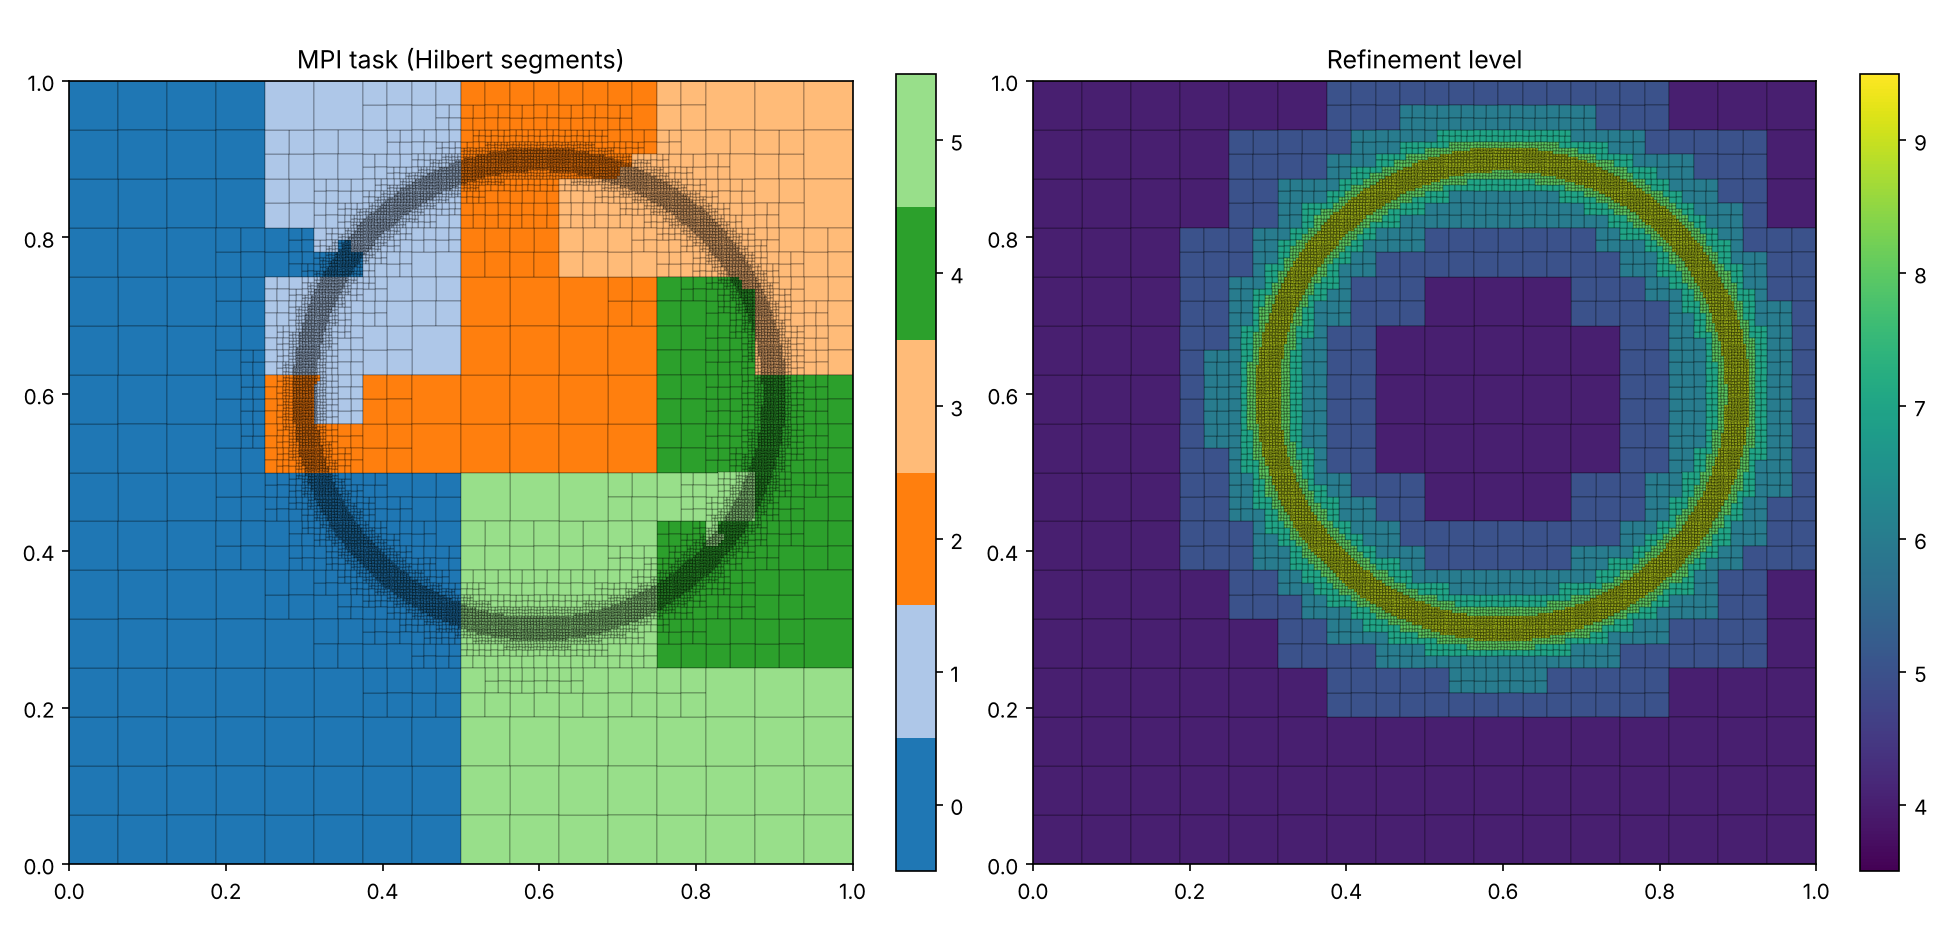
\includegraphics[width=0.9\textwidth]{amr_grid}
\caption{An \cls{AdaptiveMPIGrid} from its example (\file{AdaptiveMPIGrid/example}): a 2D grid refined around a ring from level 4 to level 9
with 2:1 balance, on 6 MPI tasks. \emph{Left:} the task owning each leaf, contiguous segments of the Peano--Hilbert curve.
\emph{Right:} the refinement level.}
\label{fig:mg-amr}
\end{figure}


\section{Validation}\label{sec:mg-validation}

\begin{validation}[Validation: uniform grids]
\file{tests/test_multigrid.cpp} on 1, 2 and 4 tasks: the finite-difference helpers against analytic derivatives (orders 1--4);
Poisson with a white-noise source reduces the residual by more than a factor 5 per V-cycle (2+2 sweeps); a DGP-type equation
with mixed derivatives converges with the cube ordering and the mean residual subtracted; the $f(R)$ cubic, equal fifth forces
from the \code{sqrt} and \code{log} methods, and convergence of \code{sqrt} for $|f_{R0}|=10^{-6}$ at $a=0.5$ (where \code{log}
gives NaN) and for $n=2$; the symmetron (zero field before symmetry breaking, linear theory for a small cosine perturbation,
screening in a halo, the generalised $(N,M)$); the dilaton (the effective-potential minimum for $r=1$ and $3/2$, linear theory,
the exact discrete solution of a strongly nonlinear sine profile of Brax et al.\ \cite{Brax2012}, screening, the warm start); DGP
with a clustered field; and every termination status. \file{tests/test_multigrid_domain.cpp}: the same solutions on slabs and on
every pencil layout, with the $2D+1$ and $3^D$ stencils and a fourth-order one.
\end{validation}

\begin{validation}[Validation: adaptive grids]
Poisson ($\nabla^2\phi=\delta$, periodic, Gaussian $\phi$) and $\nabla^2u-500u^3=s$ (Dirichlet), refined around the peak: in 2D
the rms error is $6.2\times10^{-5}$ and $6.7\times10^{-5}$ for AMR levels 4--8 against $6.1\times10^{-5}$ and
$6.9\times10^{-5}$ for the uniform level 8, and converges at second order; the residual drops by 0.12--0.21 per V-cycle. DGP for a
compensated spherical overdensity with an exact force: rms force error $2.6\times10^{-3}$ of the peak force for AMR levels 4--7
(second order, 2.35), identical on 1--4 tasks, and on a uniform $32^3$ grid equal to \cls{DGPSolverCosmology} to
$7\times10^{-11}$. Dilaton (\file{examples/AMRDilatonExample.cpp}): the same overdensity, $A_2=5\times10^5$, $\xi=10^{-3}$, screened in
the centre ($w=0.16$ for $r=1$), against a radial Newton solution: rms errors of $w$ and of the force (of the peak) $1.8\times10^{-3}$
and $1.1\times10^{-2}$ on the uniform level 6, $1.9\times10^{-3}$ and $1.2\times10^{-2}$ for AMR levels 4--6 (5\% of the leaves), $5\times10^{-4}$
and $3.6\times10^{-3}$ for levels 5--7 (order 1.93 and 1.75); on a uniform $32^3$ grid ($\ln w$ from $-0.03$ to 10.1) $\Phi_F$ equals
\cls{DilatonSolverCosmology} to $5\times10^{-14}$; a first solve from $w=1$ in a peak with $1+\delta=2\times10^4$ resolved one level
below the finest converges in 4 V-cycles. Solutions are independent of the number of tasks (1--13) and clean under AddressSanitizer.
\end{validation}

\begin{validation}[Exact against approximate screening]
In a standalone comparison (not a regression test) for $f(R)$ on a $256^3$ grid of a $64\Mpch$ GR snapshot, the screening approximation of \file{SimulationCode} agrees with the
exact fifth force to 1--3\% in cells below the critical potential for F5 at $z=0$ and to 0.2\% for F4, but over-screens once a
large fraction of the volume has $|\Phi_N|$ above it (F6, F5 at $z=1$). Solving on a grid twice coarser than the force grid
keeps the total force source within 1\% for $k<2.3\hMpc$ but loses the fifth force above the coarse Nyquist frequency
(\cref{ch:mg-simulations}).
\end{validation}

\begin{figure}[htbp]
\centering
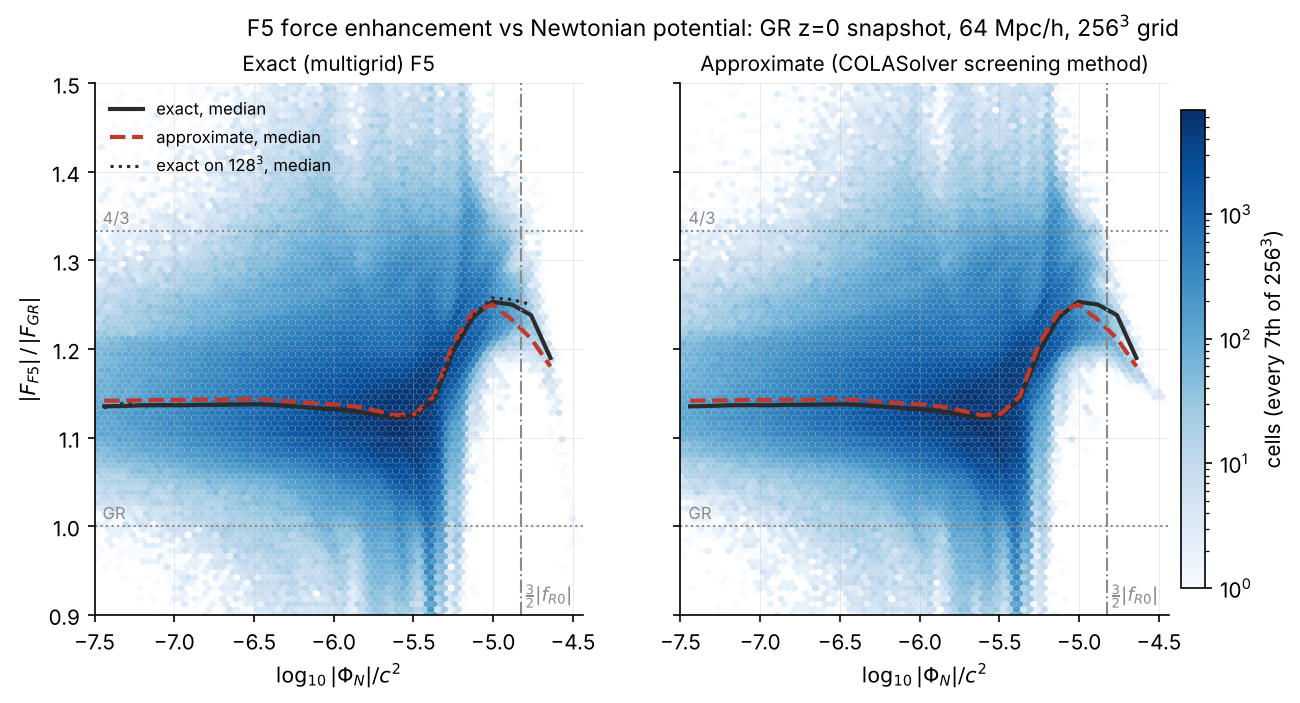
\includegraphics[width=\textwidth]{mg_f5_exact_vs_approx}
\caption{The F5 ($|f_{R0}|=10^{-5}$) force enhancement $|F_{F5}|/|F_{\rm GR}|$ against the Newtonian potential of the cell for a GR $z=0$
snapshot ($64\Mpch$, $256^3$ grid): the exact multigrid solution (\emph{left}) and the screening approximation of \file{SimulationCode}
(\emph{right}), with the medians of both (and of the exact solution on $128^3$). Unscreened cells have the linear enhancement
$\approx1.14$ at these scales (4/3 is the small-scale limit); screening sets in near $|\Phi_N|/c^2\sim\frac32|f_{R0}|$. A standalone
comparison, not a regression test.}
\label{fig:mg-f5}
\end{figure}


\chapter{Input, output and utilities}\label{ch:io-utilities}
\chapterstatus{written}{2026-11-15}

Snapshot readers and writers, plain-text tables, parameter files, physical units, timing and memory instrumentation,
the performance suite, the Python interfaces and a few smaller utilities.

\begin{modulebox}{I/O}
\nsp{FML::FILEUTILS}: \file{GadgetUtils/GadgetUtils.h} (\cls{GadgetReader}, \cls{GadgetWriter}),
\file{GadgetUtils/GadgetUtilsHDF5.h}, \file{RamsesUtils/RamsesUtils.h} (\cls{RamsesReader}), \file{FileUtils/FileUtils.h}
(\code{loadtxt}, \ldots), \file{FileUtils/DataPath.h} (\code{fml_file}); the program \file{RamsesUtils/ramses2pk}.\par
Tests: \file{tests/test_gadget.cpp}, \file{tests/test_ramses.cpp}, \file{tests/test_utils.cpp}.
\end{modulebox}
\begin{modulebox}{Parameters and units}
\file{ParameterMap/ParameterMap.h} (\cls{ParameterMap}), \file{LuaFileParser/LuaFileParser.h} (\cls{LuaFileParser}),
\nsp{FML::UTILS}: \file{Units/Units.h} (\nsp{SI}, \cls{ConstantsAndUnits}).\par
Documentation: \file{Units/README.md}. Tests: \file{tests/test_lua.cpp}, \file{tests/test_utils.cpp}, \file{tests/test_units_odr.cpp}.
\end{modulebox}
\begin{modulebox}{Instrumentation and interfaces}
\file{Timing/Timer.h}, \file{Timing/Timings.h}, \file{MemoryLogging/MemoryLogging.h}, \file{Performance/} (counters and the
benchmark runner), \file{Plotting/Matplotlibcpp.h}, \file{Chunkpix/Chunkpix.h}, \file{PythonAnalysis/} (\code{fml_analysis}),
\file{MakePythonWrapper/}, \file{HaloModel/PythonWrapper/}, \file{Visualization/} (projections, colour maps, a PNG writer),
\file{ExampleData/} (small inputs generated in code).\par
Documentation: \file{Performance/README.md}, \file{PythonAnalysis/README.md}, \file{Visualization/README.md}.
\end{modulebox}

\section{Snapshot formats}\label{sec:io-snapshots}

\paragraph*{GADGET binary} \cite{Springel2005}. \cls{GadgetReader} reads format 1 and format 2 (blocks preceded by a label block)
files of either endianness (detected and swapped), positions and velocities in float or double, 4- or 8-byte IDs (from the block
size) and the MASS block (types with zero \code{MassTable} entry, stored with \code{set_mass}); empty files are skipped and unknown
format-2 blocks ignored. Positions are returned in $[0,1)$ (scaled by the box, with a factor for files in kpc/$h$), velocities as
peculiar velocities in km/s (the file holds $v/\sqrt a$), the family/type is set if the particle has it (otherwise all are dark
matter), and with MPI each task can keep only the particles in its domain while reading all files. \cls{GadgetWriter} writes one file
per task with 4-byte IDs unless an ID or the total does not fit, several species per file with their \code{MassTable} masses
($\Omega_{\rm type}\rho_{\rm crit}B^3/N_{\rm type}$) or per-particle masses; blocks above $2^{31}$ bytes (the limit of the format) are an
error.

\paragraph*{GADGET HDF5.} \file{GadgetUtilsHDF5.h} (with \code{USE_HDF5}) reads and writes the HDF5 layout of GADGET-2/3/4, AREPO,
GIZMO and SWIFT (\code{/Header} attributes and \code{/PartTypeN/Coordinates}, \code{Velocities}, \code{ParticleIDs}, \code{Masses}), in
one or several files, with the same interface and conventions; velocity units in the file are converted to km/s.

\paragraph*{RAMSES} \cite{Teyssier2002}. \cls{RamsesReader} reads dark-matter particle files (positions, velocities in km/s from
\code{unit_l}/\code{unit_t}, masses, IDs, levels, families and tags as the particle provides them) from the header or the
\file{part_file_descriptor.txt}, keeping only the local domain if asked, and writes the \file{ic_deltab} initial-condition file.
\file{ramses2pk} computes power spectra directly from a RAMSES output.

\paragraph*{Plain text.} \code{loadtxt} and its variants read whitespace-separated numbers (comments with \#, ! or /; \code{nan},
\code{inf} and denormals), with a fixed or variable number of columns, a subsample fraction, or two extracted columns; malformed lines
are errors with the line number. \code{fml_file} resolves data files of the library from \code{FML_DIR}, the compiled
\code{FML_ROOT_DIR} or a relative path.

Grids and particle containers have raw checkpoints (\code{dump_to_file}, \code{load_from_file}; \cref{ch:grids-fft,ch:particles}).

\section{Parameters}\label{sec:io-parameters}

\cls{ParameterMap} is a map from names to typed values (string, int, bool, double and vectors of int and double, a
\code{std::variant}): \code{get<T>(name)} throws if the parameter is missing or of another type, and \code{get<T>(name, fiducial)}
returns the fiducial value only if the parameter is missing (a wrong type is still an error). \cls{LuaFileParser} reads Lua scripts as
parameter files (the format of \file{SimulationCode}, \cref{ch:simulation-code}): \code{read_int}, \code{read_double},
\code{read_string}, \code{read_bool} and arrays, each \code{required} or \code{optional} with a default. A parameter that is set with the
wrong type (1 for a boolean, 2.5 for an integer, a string in an array of numbers) is always an error, and reading many unset optional
parameters no longer corrupts the Lua stack. Being Lua, parameter files can compute values and use loops and conditions.

\section{Units and constants}\label{sec:io-units}

\file{Units.h} is the single source of physical constants: \nsp{FML::UTILS::SI} holds compile-time SI values (units, derived and
astronomical units, fundamental constants, recombination energies and rates, $H_0/h$ in s$^{-1}$; the ionisation energies are in joules),
and \cls{ConstantsAndUnits} gives all constants in a chosen system (\code{"SI"}, \code{"Planck"}, \code{"ParticlePhysics"},
\code{"Cosmology"}: Mpc, Hubble time, solar masses and kelvin, or user factors), derived from the same table. The Einstein--Boltzmann
solver's \code{Constants} namespace is an alias to it (\cref{ch:conventions}). The year is the 365.25-day Julian year.

\section{Instrumentation}\label{sec:io-instrumentation}

\paragraph*{Timing.} \cls{Timer} is a stopwatch; \cls{Timings} accumulates labelled timings over restarts (a repeated end does not count
twice) and prints a summary; \file{SimulationCode} reports the time of every part of a step with it.

\paragraph*{Memory.} With \code{MEMORY_LOGGING} the containers of the library use a logging allocator that records every allocation above a
minimum size with its label (grids and particle containers label themselves), keeps the current and peak memory and their history, and
prints the range over tasks; it is thread safe and bounded in the number of tracked allocations. \file{SystemMemory.h} gives the resident
set size (\cref{sec:par-communication}).

\paragraph*{Performance suite.} \file{Performance/} measures representative operations with full provenance, separately from the
correctness tests: an FFT round trip, grid copies and empty clones, Fourier resampling, particle migration and selected bispectrum
configurations, each validated outside the timed region. The runner (\file{run.py}) runs every case, rank and thread count in a fresh
process and stores JSON reports, raw logs, the argument vectors and a manifest (host, CPU affinity, OpenMP settings, the executable's
SHA-256). Opt-in counters (\code{FML_ENABLE_PERFORMANCE_COUNTERS}) count FFTW plan creations, transforms, grid allocations and copies, and
the payload bytes and messages of the transports.

\section{Python}\label{sec:io-python}

\begin{itemize}
\item \code{fml_analysis} (\file{PythonAnalysis/}, pybind11): a serial catalogue interface to the spatial statistics of
      \cref{ch:configuration-space}: \code{Catalogue(positions, boxsize)} with $k$-nearest-neighbour distances and CDFs, sphere counts and
      counts-in-cells summaries for query points, on a KD-tree, with NumPy arrays in and out, copies of all inputs and the GIL released during
      the C++ work. It does not initialise MPI or FFTW.
\item The halo-model wrapper (\file{HaloModel/PythonWrapper/}, pybind11) exposes \cls{HaloModel} (\cref{ch:halo-model}).
\item \file{MakePythonWrapper/} shows how to wrap any FML function with SWIG and NumPy arrays.
\end{itemize}

\section{Pictures}\label{sec:io-visualization}

\file{Visualization} makes pictures of fields and particles from C++ with no dependencies, for a quick look at a run or
frames of a movie. \code{project_grid} projects a slab of an \cls{FFTWGrid} or \cls{PencilGrid} along an axis (the sum or
the mean over the cells whose positions $i/N_{\rm mesh}$ are in a periodic slab) and \code{project_particles} the particles
(NGP or CIC, mass weighted when they have masses), giving the same \cls{Image} on every task. \cls{ColorScale} maps the
values linearly, logarithmically or symmetrically about zero, with fixed limits or percentiles of the image, onto a colour
map: magma, inferno, viridis, plasma and cividis (the matplotlib tables), coolwarm (diverging \cite{Moreland2009}), grey
and cubehelix \cite{Green2011} (a suffix \code{_r} reverses them). \code{write_png} has its own deflate (per-row filters,
LZ77 and fixed Huffman codes, stored blocks for noise), and \code{write_npy} writes the values for numpy.
\file{Analysis/Images.h} builds on it for the images of \file{SimulationCode} and SnapshotAnalyzer
(\cref{sec:sim-analysis,sec:sa-program}).

\begin{cppcode}[A projected slab as a PNG]
#include <FML/Visualization/Visualization.h>
using namespace FML::VISUALIZATION;
Image image = project_grid(density, 2, 0.45, 0.1);   // a slab of 10% of the box along z (mean)
if (FML::ThisTask == 0)
    write_png("density.png", image, "magma", ColorScale::automatic_log());
\end{cppcode}

\section{Other utilities}\label{sec:io-other}

\file{ExampleData} generates the small inputs the examples and tests use (a clustered particle box, linear spectra and
tables) in code, so that no data files are needed.

\code{Matplotlibcpp} (adapted from matplotlib-cpp) makes matplotlib plots from C++. \cls{Chunkpix} (by Albert Izard) stores sparse HEALPix
\cite{Gorski2005} maps: the $12N_{\rm side}^2$ pixels are split into $12N_{\rm side,chunk}^2$ chunks and only the chunks that are written to are
allocated; with NEST ordering a chunk is a compact patch, so a partial-sky map allocates about that fraction. It holds the lightcone maps of
\file{SimulationCode} (\cref{ch:weak-lensing}).

\begin{validation}[Validation: I/O and utilities]
\file{tests/test_gadget.cpp}: write and read back on several tasks (positions, peculiar velocities, IDs, header), several species and their
masses, 8-byte IDs, small and empty files, per-particle masses, big- and little-endian files and format 2 with an extra block, HDF5 (including
SWIFT's three-element box size and snapshots with different numbers of files). \file{tests/test_ramses.cpp}: synthetic RAMSES snapshots
(domain reading, units for both Mpc conventions of RAMSES, empty CPU files, a particle at $x=1$, the descriptor file). \file{tests/test_lua.cpp}:
many unset parameters, defaults, arrays and the wrong-type errors. \file{tests/test_utils.cpp}: \code{loadtxt} edge cases, the random generators,
the memory log with many allocations and threads, timings, \cls{ParameterMap} types and the unit systems.
\file{Visualization/tests}: the projections against direct sums (slabs and pencils, every axis, periodic slabs, 1, 2 and
4 tasks), the particle weights and mass conservation, the colour maps and scales, and the PNG and \code{.npy} files read
back with Python's standard library (every pixel compared).
\end{validation}


\part{The homogeneous universe and linear theory}\label{part:linear}
\chapter{The background cosmology}\label{ch:background}
\chapterstatus{written}{2026-11-17}

The expansion history of a homogeneous and isotropic universe is the input of almost everything else in the library:
the recombination rates compete with the expansion rate, the perturbation equations contain $\Hp$ and its derivatives,
the line-of-sight integrals need the distance to the last-scattering surface, simulations need $H(a)$ for their time
steps and growth factors, and survey and lensing calculations need distances. \fml{} has one implementation of the
background, \cls{Background} in \file{Cosmology/Background}, which all these users share. This chapter describes its
equations, the species and theories of gravity it is built from, the model library and the numerical methods.

\begin{modulebox}{Cosmology/Background}
Namespace \nsp{FML::COSMOLOGY::BACKGROUND}; header-only (needs \file{Spline}, \file{ODESolver}, \file{Math}, GSL).\par
Core: \file{Background.h} (abstract interface, times and distances), \file{ComponentBackground.h} (species + field
equations), \file{TabulatedBackground.h}, \file{FunctionBackground.h}, \file{BackgroundParameters.h}.\par
Species and gravity: \file{Species.h}, \file{FieldEquations.h}, \file{FieldEquation_GeneralRelativity.h},
\file{FieldEquation_DGP.h}, \file{FieldEquation_BransDicke.h}.\par
Models: \file{BackgroundModel_<name>.h} for LCDM, w0wa, DGP, Quintessence, EDE, Axion, BransDicke,
CoupledQuintessence, CubicGalileon, DarkScattering, IDE, Tabulated, HorndeskiTable; the registry \file{Presets.h}.\par
Solver interface: \file{BackgroundCosmology.h/.cpp} (SI adapter used by the Einstein--Boltzmann solver),
\file{CosmologyParameters.h/.cpp}, \file{BBN.h/.cpp}.\par
Documentation: \file{Cosmology/Background/README.md}. Tests: \file{Cosmology/Background/tests}.
\end{modulebox}

\section{The Friedmann equations}\label{sec:bg-friedmann}

On large scales the universe is described by the Friedmann--Lema\^itre--Robertson--Walker metric,
\begin{equation}
\dd s^2=-c^2\dd t^2+a^2(t)\left[\frac{\dd r^2}{1-Kr^2}+r^2\dd\Omega^2\right],
\end{equation}
with the scale factor $a(t)$, normalised to $a_0=1$ today, and the spatial curvature $K$ ($K>0$ closed, $K<0$ open).
Homogeneity and isotropy restrict the matter to perfect fluids with energy densities $\rho_ic^2$ and pressures $p_i$.
In general relativity Einstein's equations reduce to the Friedmann equation and the acceleration equation,
\begin{equation}
H^2\equiv\left(\frac{\dot a}{a}\right)^2=\frac{8\pi G}{3}\sum_i\rho_i-\frac{Kc^2}{a^2},\qquad
\frac{\ddot a}{a}=-\frac{4\pi G}{3}\sum_i\left(\rho_i+\frac{3p_i}{c^2}\right).
\label{eq:bg-friedmann}
\end{equation}
Their combination is the continuity equation. With the time variable $x=\ln a$ used throughout the library and
$'=\dd/\dd x$,
\begin{equation}
\rho_i'=-3\left(\rho_i+\frac{p_i}{c^2}\right)\qquad\text{(uncoupled species)},
\label{eq:bg-continuity}
\end{equation}
which for a constant equation of state $w_i=p_i/(\rho_ic^2)$ gives $\rho_i\propto a^{-3(1+w_i)}$. Species that
exchange energy (interacting dark energy, coupled quintessence) replace \cref{eq:bg-continuity} by their own
equations, but the sum over all species still obeys it.

Measuring densities in units of today's critical density $\rho_{c0}=3H_0^2/(8\pi G)$ and writing $E=H/H_0$, the
Friedmann equation of GR becomes
\begin{equation}
E^2(x)=\sum_i\frac{\rho_i(x)}{\rho_{c0}}+\Om_ke^{-2x},\qquad \Om_k=-\frac{Kc^2}{H_0^2},
\label{eq:bg-E2}
\end{equation}
and $E(0)=1$ is the closure condition $\sum_i\Om_i+\Om_k=1$. For the standard species this is the familiar
\begin{equation}
E^2=\Om_\gamma e^{-4x}+\Om_\nu e^{-4x}+(\Om_b+\Om_{\rm cdm})e^{-3x}+\frac{\rho_{\nu,\rm massive}}{\rho_{c0}}
+\Om_ke^{-2x}+\Om_\Lambda .
\end{equation}
The density parameters at time $x$ are $\Om_i(x)=\rho_i(x)/(\rho_{c0}E^2)$, and curvature is reported as
$\Om_k(x)=\Om_ke^{-2x}/E^2$, so that $\sum_i\Om_i(x)+\Om_k(x)=1$ in GR (in Brans--Dicke gravity the scalar field
has no species and the sum differs from one, \cref{sec:bg-bransdicke}). From $E$ and its logarithmic derivative the
library derives
\begin{equation}
\Hp\equiv aH,\qquad w_{\rm eff}=-1-\frac23\frac{\dd\ln E}{\dd x},\qquad q=-\frac{\ddot aa}{\dot a^2}=-1-\frac{\dd\ln E}{\dd x},
\end{equation}
the effective equation of state of the total (curvature counted as a fluid with $w=-1/3$) and the deceleration
parameter. The onset of acceleration is where $\Hp'=0$.

\paragraph*{Radiation.} The photons are a blackbody of temperature $T_{\rm CMB}$ (default $2.7255$\,K), so
\begin{equation}
\Om_\gamma=\frac{\pi^2}{15}\frac{(k_BT_{\rm CMB})^4}{(\hbar c)^3}\frac{1}{\rho_{c0}c^2}.
\end{equation}
Neutrinos decoupled before electron--positron annihilation, after which $T_\nu=(4/11)^{1/3}T_\gamma$; with the
fermionic factor $7/8$ each massless species contributes $\frac78(4/11)^{4/3}\Om_\gamma$. The effective number
$N_{\rm eff}$ (default $3.046$; $3.044$ is the modern value) counts \emph{all} neutrinos. A massive species of
temperature $T_{\rm ncdm}=0.71611\,T_{\rm CMB}$ (CLASS's default) contributes
\begin{equation}
N_{\rm ncdm}=\left(\frac{T_{\rm ncdm}/T_{\rm CMB}}{(4/11)^{1/3}}\right)^4=1.0132
\end{equation}
to $N_{\rm eff}$, and the remaining $N_{\rm eff}-n_{\rm massive}N_{\rm ncdm}$ species are massless. This is the
convention of CLASS and of the Einstein--Boltzmann solver (\cref{ch:linear-perturbations}); with it a massive species
has $\Om_\nu h^2=m_\nu/93.14\,$eV today.

\section{Times, horizons and distances}\label{sec:bg-distances}

\paragraph*{Clocks.} Cosmic time $t$, conformal time $\eta$ and the comoving distance $\chi$ to an object at $x$
obey
\begin{equation}
\frac{\dd t}{\dd x}=\frac{1}{H},\qquad \frac{\dd\eta}{\dd x}=\frac{c}{\Hp}=\frac{c}{aH},\qquad \chi(x)=\eta_0-\eta(x).
\label{eq:bg-clocks}
\end{equation}
$\eta(x)$ is the particle horizon, the comoving distance light has travelled since the big bang; $c/\Hp$ is the
comoving Hubble radius, and a mode of wavenumber $k$ is outside the horizon while $ck<\Hp$. In an era dominated by a
single component with $\rho\propto a^{-n}$,
\begin{equation}
\frac{\Hp'}{\Hp}=1-\frac n2,\qquad \frac{\Hp''}{\Hp}=\left(1-\frac n2\right)^2,\qquad
\frac{\eta\Hp}{c}=\frac{2}{n-2}\;(n>2),\qquad t=\frac{2}{nH},
\label{eq:bg-single}
\end{equation}
i.e.\ $\eta\Hp/c=1$ in radiation domination and $2$ in matter domination. These limits are both the initial
conditions of the integration and the main tests of it.

\paragraph*{Distances.} In a curved universe the comoving transverse distance of an object at comoving radial
distance $\chi$ is
\begin{equation}
D_M=\sin_K(\chi)=\begin{cases}\sin(\sqrt K\chi)/\sqrt K & K>0\ \text{(closed)}\\ \chi & K=0\\
\sinh(\sqrt{-K}\chi)/\sqrt{-K} & K<0\ \text{(open)}\end{cases},\qquad
\cot_K(\chi)=\frac{\dd\ln\sin_K\chi}{\dd\chi},
\label{eq:bg-sinK}
\end{equation}
and the angular diameter, luminosity and Hubble distances are
\begin{equation}
D_A=\frac{D_M}{1+z},\qquad D_L=(1+z)D_M,\qquad D_H=\frac{c}{H}.
\end{equation}
$\sin_K$ and $\cot_K$ are evaluated with series expansions when $|K\chi^2|<10^{-4}$, so that every quantity is
smooth through $\Om_k=0$; the same functions enter the line-of-sight integrals and the truncation of the Boltzmann
hierarchies in curved universes (\cref{ch:linear-perturbations,ch:cmb-spectra}).

\begin{implementation}[Implementation: tabulating times and distances]
A derived class provides the \emph{virtual core} --- $E(x)$, $\dd\ln E/\dd x$, $\Om_i(x)$, the parameters and the
valid range $[x_{\min},x_{\max}]$ (default $a\in[10^{-10},10]$) --- and calls \code{finalize()} at the end of its
constructor. \code{finalize()} integrates \cref{eq:bg-clocks} once:
\begin{itemize}
\item on a grid in $x$ with a node at $x=0$ and \code{points_per_unit_x} (default 200) points per unit $x$, with
      5-point Gauss--Legendre quadrature on each interval;
\item starting from the exact power-law solution at $x_{\min}$, which must lie in an era with $E\propto a^{-n/2}$,
      $n>2$: $\eta(x_{\min})=c/[aH_0E(n/2-1)]$ and $t(x_{\min})=2/(nH)$ (\cref{eq:bg-single});
\item computing $\chi=\eta_0-\eta$ by summation from $x=0$, which avoids the cancellation of two large numbers at
      low redshift.
\end{itemize}
$\ln\eta$, $\ln t$ and $\chi$ are stored as cubic splines, and the inverse $x(\chi)$ is splined on the reversed
arrays. In the far future of models whose $E$ grows very fast (e.g.\ CPL with $w_a>0$) $\chi$ stops changing in
double precision, and the inverse covers only the part where $\chi$ is strictly monotonic. Everything else
(distances with curvature, $a$- and $z$-versions of all functions, \code{info()}, \code{output()}) is non-virtual and
shared by all backgrounds. A \cls{Background} is immutable after construction and shared as
\code{std::shared_ptr<const Background>}; all methods are \code{const} and thread-safe.
\end{implementation}

\paragraph*{Units.} $E$ is dimensionless. The conformal time $\eta$, the comoving distance $\chi$ and all other distances
are in $\Mpch$, with $c/H_0=2997.92458\,\Mpch$. Cosmic time is in Gyr (\code{t_Gyr}, \code{age_Gyr}) or in units of $1/H_0$
(\code{t_H0}); the curvature
\code{K_hmpc2()} is in $(h/\mathrm{Mpc})^2$. Every function exists in versions taking $x$, $a$ or $z$.

\begin{figure}[htbp]
\centering
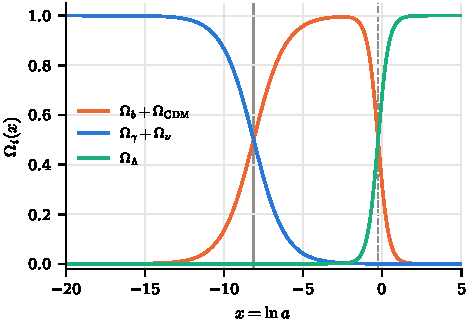
\includegraphics[width=0.49\textwidth]{m1_Omegas}\hfill
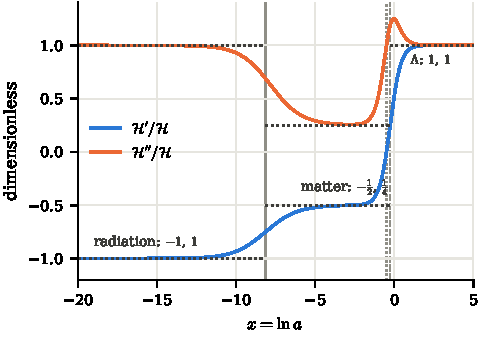
\includegraphics[width=0.49\textwidth]{m1_Hp_derivatives}
\caption{\emph{Left:} density parameters of radiation, matter and the cosmological constant in the fiducial
$\Lambda$CDM model ($h=0.67$, $\Om_b=0.05$, $\Om_{\rm cdm}=0.267$). \emph{Right:} $\Hp'/\Hp$ and $\Hp''/\Hp$ with
the analytic values of \cref{eq:bg-single} in each era (dotted). Vertical lines mark radiation--matter equality,
matter--$\Lambda$ equality and the onset of acceleration. From the Einstein--Boltzmann solver report.}
\label{fig:bg-omegas}
\end{figure}

\section{Species}\label{sec:bg-species}

A \cls{ComponentBackground} is a list of species (\file{Species.h}) and a theory of gravity
(\cref{sec:bg-field-equations}). A species gives its energy density $\rho(x)$ and pressure $p(x)$ in units of
$\rho_{c0}$ (pressure in $\rho_{c0}c^2$), its derivative $\rho'(x)$ (default: \cref{eq:bg-continuity}) and its second
derivative $\rho''$ (used by the perturbations of some theories; analytic for all species in the library, otherwise a
5-point central difference of $\rho'$ with step $10^{-3}$). Each species belongs to a component (\code{Baryons},
\code{CDM}, \code{Photons}, \code{MasslessNeutrinos}, \code{MassiveNeutrinos}, \code{DarkEnergy}, \code{Axions},
\code{Other}, \ldots), and $\Om(c,x)$ sums the species of component $c$. Matter, \code{Omega_m}, is baryons + CDM +
massive neutrinos (including their small relativistic part); an ultralight axion is a separate component, included
in \code{Omega_m_axion}. The function \code{standard_species(p)} gives the species every model has: baryons, CDM,
photons, massless neutrinos and one species per entry of \code{m_nu_eV}.

\subsection{Power laws and CPL dark energy}

\cls{PowerLawSpecies} has $\rho=\Om_0a^{-n}$ and $p=(n/3-1)\rho$: baryons and CDM ($n=3$), photons and massless
neutrinos ($n=4$) and a cosmological constant ($n=0$). \cls{CPLDarkEnergy} has the equation of state of Chevallier,
Polarski and Linder \cite{ChevallierPolarski2001,Linder2003}, $w(a)=w_0+w_a(1-a)$, for which \cref{eq:bg-continuity}
integrates to
\begin{equation}
\rho_{\rm DE}=\Om_{\rm DE}\,a^{-3(1+w_0+w_a)}e^{-3w_a(1-a)},\qquad
\rho_{\rm DE}''=3w_aa\,\rho_{\rm DE}+9(1+w)^2\rho_{\rm DE}.
\end{equation}

\subsection{Massive neutrinos}\label{sec:bg-ncdm}

Massive neutrinos decoupled while relativistic and keep the relativistic Fermi--Dirac distribution
$f_0(q)=1/(e^q+1)$ in the comoving momentum $q=ap/(k_BT_{\nu0})$ also after they become non-relativistic
\cite{LesgourguesPastor2006}. With the mass in units of the temperature, $M(x)=m_\nu c^2a/(k_BT_{\nu0})$, and the
comoving energy $\epsilon=\sqrt{q^2+M^2}$, one species (neutrino and antineutrino) has
\begin{gather}
\rho=C\,a^{-4}I_\rho(M),\qquad p=C\,a^{-4}I_p(M),\qquad \mathfrak p=C\,a^{-4}I_{pp}(M),\qquad
C=\frac{15}{\pi^4}\left(\frac{T_{\rm ncdm}}{T_{\rm CMB}}\right)^4\Om_\gamma,\\
I_\rho=\int_0^\infty q^2\epsilon f_0\,\dd q,\qquad I_p=\int_0^\infty\frac{q^4}{3\epsilon}f_0\,\dd q,\qquad
I_{pp}=\int_0^\infty\frac{q^6}{3\epsilon^3}f_0\,\dd q .
\end{gather}
$I_\rho(0)=7\pi^4/120$ reproduces the massless density $\frac78(T_\nu/T_\gamma)^4\Om_\gamma a^{-4}$. The
\emph{pseudo-pressure} $\mathfrak p$ of Lesgourgues and Tram \cite{LesgourguesTram2011} gives the derivative of the
pressure, $\dd I_p/\dd\ln M=I_{pp}-I_p$, hence
\begin{equation}
\rho'=-3(\rho+p),\qquad p'=-(5p-\mathfrak p),\qquad \rho''=-3(\rho'+p').
\end{equation}
The neutrinos become non-relativistic around $M\approx3$, i.e.\ $1+z_{\rm nr}\approx M_0/3$; the mean energy per mass
is $\langle E/m\rangle=I_\rho/(\frac32\zeta(3)M)\to1$.

\begin{implementation}[Implementation: Fermi--Dirac integrals]
$I_\rho$, $I_p$ and $I_{pp}$ are tabulated once (Simpson's rule in $q$ on $[0,60]$, splined in $\ln M$ on
$[10^{-4},10^7]$) and continued with their series outside the table:
\begin{align*}
M\ll1:&\quad I_\rho\simeq I_{\rho,0}+\tfrac{\pi^2}{24}M^2,\quad I_p\simeq \tfrac13I_{\rho,0}-\tfrac{\pi^2}{72}M^2,
\quad I_{pp}\simeq\tfrac13I_{\rho,0}-\tfrac{\pi^2}{24}M^2,\\
M\gg1:&\quad I_\rho\simeq\tfrac32\zeta(3)M+\tfrac{45}{4}\frac{\zeta(5)}{M},\quad I_p\simeq\tfrac{15}{2}\frac{\zeta(5)}{M},
\quad I_{pp}\simeq\tfrac{945}{4}\frac{\zeta(7)}{M^3}.
\end{align*}
The tests compare the tables with direct integration to $10^{-10}$. Degenerate species (same mass and temperature)
are one species with the summed density; species of different masses are separate. The helper
\code{FermiDiracSampler} draws momenta from $q^2f_0(q)$ by inverting its CDF, which SimulationCode uses for the
thermal velocities $v=qc/M_0$ of neutrino particles (\cref{ch:simulation-code}).
\end{implementation}

\subsection{Scaled species}

\cls{ScaledSpecies} multiplies another species by a constant. It implements other normalisations of the density
parameters, such as those of Brans--Dicke gravity (\cref{sec:bg-bransdicke}); \code{massive_neutrino_species()}
unwraps (nested) scaled species to reach the underlying neutrinos and their factor.

\section{Theories of gravity}\label{sec:bg-field-equations}

\cls{FieldEquations} gives $E^2(x)$ and $\dd E^2/\dd x$ from the species. Theories with their own background degrees
of freedom solve them in \code{init()}, which the \cls{ComponentBackground} constructor calls once, after which the
constructor checks the closure $E(0)=1$.

\paragraph*{General relativity.} $E^2=\sum_i\rho_i/\rho_{c0}+\Om_ke^{-2x}$ (\cref{eq:bg-E2}).

\paragraph*{DGP.} In the Dvali--Gabadadze--Porrati braneworld \cite{Dvali2000} gravity leaks into a fifth dimension
on scales larger than the crossover scale $r_c$. For a flat brane the Friedmann equation is
\begin{equation}
H^2-\epsilon\frac{Hc}{r_c}=\frac{8\pi G}{3}\rho\quad\Longrightarrow\quad
E=\epsilon\sqrt{\Om_{rc}}+\sqrt{\Om_{rc}+\rho/\rho_{c0}},\qquad \Om_{rc}=\frac{c^2}{4r_c^2H_0^2},
\end{equation}
with $\epsilon=+1$ on the self-accelerating branch (sDGP, which accelerates without dark energy) and $\epsilon=-1$ on
the normal branch (nDGP, which needs dark energy; the library adds a cosmological constant fixed by $E(0)=1$). With
\code{dgp_lcdm_background} the expansion is that of $\Lambda$CDM and only the perturbations are modified, the
``nDGP'' of $N$-body work \cite{Schmidt2009}.

\subsection{Jordan--Brans--Dicke gravity}\label{sec:bg-bransdicke}

In Brans--Dicke gravity \cite{BransDicke1961} with a cosmological constant (Jordan frame),
\begin{equation}
S=\frac{1}{16\pi G}\int\dd^4x\sqrt{-g}\left[\phi R-\frac{\omega}{\phi}(\partial\phi)^2-2\Lambda\right]+S_m,
\end{equation}
gravity couples to matter with the strength $G/\phi$, and the constant measured in a Cavendish experiment is
$G_{\rm eff}=G\phi_*/\phi$ with $\phi_*=(4+2\omega)/(3+2\omega)$; $\omega\to\infty$ is GR. With $F=\phi$,
$F_x=\dd\phi/\dd x$, densities in units of $\rho_{c0}=3H_0^2/(8\pi G_*)$ and $g=G/G_*$ (see below),
\begin{align}
E^2\left(F+F_x-\frac{\omega}{6}\frac{F_x^2}{F}\right)&=g\rho+F\Om_ke^{-2x},\\
F_{xx}&=-\left(3+\frac{\dd\ln E}{\dd x}\right)F_x+\frac{3g(\rho-3p)}{(3+2\omega)E^2}.
\end{align}
Writing $N=g\rho+F\Om_ke^{-2x}$, $D=F+F_x-\omega F_x^2/(6F)$, $y=F_x/F$, $q=1-\omega y/3$ and
$S=3g(\rho-3p)/(3+2\omega)$, the derivative of the Friedmann equation with $F_{xx}$ eliminated gives the expansion rate
\begin{equation}
\frac{\dd\ln E}{\dd x}\left[2D-qF_x\right]=\frac{N'}{N}D-F_x-q\left(\frac{S}{E^2}-3F_x\right)-\frac{\omega}{6}F_xy^2 .
\end{equation}
The field starts at rest deep in the radiation era, where $\rho-3p\simeq0$ and the decaying mode $\propto1/a$ can be
dropped. Its initial value and $\Om_\Lambda$ are found by iteration so that $\phi(0)=\phi_*/(G_{\rm eff}/G)_0$ (the
parameter \param{bd_GeffG_today}, default $1$: the Newtonian constant today is $G$) and $E(0)=1$. The scalar field is
not a species, so $\sum_i\Om_i(x)\neq1$.

\begin{table}[htbp]
\centering\small
\caption{Definitions of the density parameters in Brans--Dicke gravity: the constant $G_*$ in
$\Om_i=8\pi G_*\rho_i/(3H_0^2)$, and the value of $G$ used to convert $T_{\rm CMB}$ and the neutrino masses to
densities. The radiation and massive-neutrino densities are multiplied by $\phi_*/g$ (1 for hi\_class). The last three
describe the same physics with differently normalised $\Om_i$.}
\label{tab:bg-jbd-definitions}
\begin{tabular}{@{}llll@{}}
\toprule
Definition (SimulationCode value) & $G_*$ & $G_{\rm SI}$ & Remark \\
\midrule
\code{hi-class} (0, default) & $G$ & $G$ & as hi\_class and the Einstein--Boltzmann solver \\
\code{Gtoday} (1) & $G/\phi(0)$ & $G/\phi_*$ & $\sum\Om_i+\Om_\phi=1$ today \\
\code{Gnewton} (2) & $G/\phi_*$ & $G/\phi_*$ & SimulationCode's ``$G_N$'' \\
\code{Gbare} (3) & $G$ & $G/\phi_*$ & \\
\bottomrule
\end{tabular}
\end{table}

\section{Scalar fields}\label{sec:bg-scalar-fields}

Several dark-energy and dark-matter models are a minimally coupled scalar field $\phi$ (in units of the reduced
Planck mass $\Mpl$) with potential $V(\phi)=3H_0^2\Mpl^2\,v(\phi)$, so that $v$ is a density in units of $\rho_{c0}$.
\cls{ScalarFieldSpecies} solves the field together with the other species $\rho_o$ (everything except the field),
the curvature and an optional bare cosmological constant $\Om_L$. With $\phi_x=\dd\phi/\dd x$,
\begin{gather}
\rho_\phi=\frac{E^2\phi_x^2}{6}+v,\qquad p_\phi=\frac{E^2\phi_x^2}{6}-v,\qquad
E^2=\frac{\rho_o+\Om_ke^{-2x}+\Om_L+v}{1-\phi_x^2/6},\label{eq:bg-sf-E2}\\
\phi_{xx}=-\left(3+\frac{\dd\ln E}{\dd x}\right)\phi_x-\frac{3v_\phi}{E^2},\qquad
\frac{\dd\ln E}{\dd x}=\frac{\rho_o'-2\Om_ke^{-2x}-E^2\phi_x^2}{2E^2},\label{eq:bg-sf-kg}
\end{gather}
and $\rho_\phi'=-E^2\phi_x^2$. The field starts at $x_{\rm start}=\min(\ln10^{-10},x_{\min})$, deep in the radiation
era, at $\phi_{\rm ini}$ with $\phi_x=\code{dphidlna_ini}$ (default 0: frozen by Hubble friction).

\begin{implementation}[Implementation: the field solution and oscillating fields]
\begin{itemize}
\item The Klein--Gordon equation is integrated with GSL's RK8PD (relative error $10^{-12}$) and stored on a uniform
      grid in $x$ (spacing $0.002$) with $\phi$, $\phi_x$ and $\phi_{xx}$. Between the nodes $\phi$ and $\phi_x$ come
      from \emph{quintic Hermite} interpolation of $(\phi,\phi_x,\phi_{xx})$ at the two neighbouring nodes, whose error
      $\sim(\omega\Delta x)^6$ for a field oscillating with frequency $\omega$ in $x$ is far below that of a cubic spline
      ($10^{-5}$ in $E$ for $m/H\sim100$). $\rho$ and $p$ are computed from the interpolated $\phi,\phi_x$.
\item The integration throws if the field makes $E^2\le0$ or $\phi_x^2\ge6$.
\item \emph{Oscillating fields.} A field in a potential with a minimum eventually oscillates about it many times per
      Hubble time. Once it oscillates fast (at least 3 crossings of the minimum and the last half period shorter than
      $0.025$ in $x$, i.e.\ $m/H\gtrsim125$) it is replaced by a fluid with the cycle-averaged equation of state
      $w_{\rm osc}$, $\rho=\rho_{\rm sw}e^{-3(1+w_{\rm osc})(x-x_{\rm sw})}$. The switch is placed at an exact crossing
      of the minimum (found by bisection between nodes to $10^{-12}$ in $x$), where the instantaneous density lies on its
      cycle-averaged trend, so that the results are smooth functions of the parameters (switching at a grid node gave
      steps of $3\times10^{-4}$ in the $C_\ell$).
\item Alternatively, with \code{switch_at_mass_over_H} $=s>0$ (the ultralight axion), $s\le4$ switches at $m/H=s$
      before the first crossing, with the instantaneous density (axionCAMB's convention, $s=3$), and $s>4$ at the first
      crossing after $m/H\ge s$ (for convergence tests).
\end{itemize}
\end{implementation}

\subsection{Quintessence}

\cls{QuintessenceSpecies} has $v=V_0u(\phi)$ with the shapes
\begin{center}\footnotesize
\begin{tabular}{@{}lll@{}}
\toprule
Potential (registry name) & $u(\phi)$ & Parameters \\
\midrule
exponential (\code{quintessence}) & $e^{-\lambda\phi}$ & \param{quint_lambda}; $\lambda=0$ is $\Lambda$ \\
inverse power law (\code{quintessence_inverse_power_law}) & $\phi^{-\alpha}$ \cite{RatraPeebles1988} & \param{quint_alpha} \\
PNGB (\code{quintessence_pngb}) & $1+\cos(\phi/f)$ \cite{Frieman1995} & \param{quint_f} \\
hilltop (\code{quintessence_hilltop}) & $\left[1-(|\phi|/\mu)^p\right]^2$ \cite{DuttaScherrer2008} & \param{quint_mu}, \param{quint_p} \\
\bottomrule
\end{tabular}
\end{center}
$V_0$ is found by shooting so that $\rho_\phi(0)$ closes the budget (Brent's method on $\ln V_0$, the field has no
bare $\Lambda$). While the field does not oscillate, $\rho_\phi(0)$ increases monotonically with $V_0$; when it
oscillates before today it does not, and the root is bracketed within $e^{\pm24}$ of the frozen-field value first.

\subsection{Early dark energy}

The axion-like early dark energy of Poulin et al.\ and Smith et al.\ \cite{Poulin2019,Smith2020} has
\begin{equation}
V=m^2f^2\left[1-\cos(\phi/f)\right]^n,\qquad v=\mu\,(1-\cos\theta)^n,\quad\theta=\phi/f,\quad
\mu=\frac{m^2f^2}{3H_0^2\Mpl^2},
\end{equation}
plus a cosmological constant. The field is frozen at $\theta_i$ until $H\sim m$, then oscillates; the oscillating field
has $w_{\rm osc}=(n-1)/(n+1)$ and its energy dilutes as $a^{-6n/(n+1)}$. As in CLASS\_EDE \cite{Hill2020} the model is
specified by the maximum fraction $f_{\rm EDE}$ of $\rho_\phi/\rho_{\rm tot}$, the redshift $z_c$ where it is reached,
$\theta_i$ and $n$ (\param{ede_fEDE}, \param{ede_log10zc} or \param{ede_zc}, \param{ede_theta_i}, \param{ede_n}).
$(\ln\mu,\ln f)$ are found by a damped Newton iteration on $(\ln f_{\rm max},x_{\rm peak})=(\ln f_{\rm EDE},x_c)$,
alternated with the closure for $\Om_\Lambda$ until both converge. The initial guess uses the frozen density
$\mu u_i^n$ and the time when the force term of $\theta_{xx}=-3\mu nu^{n-1}\sin\theta/(f^2E^2)$ becomes comparable
to $3\theta_i$. For $n\le1$ the fraction never decays, and for $1<n\le2$ it grows during radiation domination and peaks
only after equality, so $(f_{\rm EDE},z_c)$ do not define the model for $z_c$ in the radiation era: the background
needs $n>1$ (as SimulationCode); the Einstein--Boltzmann solver accepts $n>1$ since the oscillating phase became a
fluid (\cref{ch:extended-models}).

\subsection{Ultralight axion dark matter}

In the mixed dark-matter model of axionCAMB \cite{Hlozek2015} a fraction \param{ax_fraction} of the dark matter is
an ultralight axion with $V=\frac12m^2\phi^2$, $v=(m/H_0)^2\phi^2/6$:
\begin{equation}
\Om_{\rm ax}=f_{\rm ax}\,\Om_d,\qquad \Om_{\rm cdm}=(1-f_{\rm ax})\,\Om_d,
\end{equation}
with $\Om_d$ the dark matter of the parameters. The field starts frozen ($m/H<0.1$ is required at the start) and
$\phi_i$ is found by a secant iteration on $\ln\phi_i$ so that $\rho(0)=\Om_{\rm ax}$ (for a test field
$\ln\rho(0)\simeq2\ln\phi_i+$const); $\Lambda$ follows from closure. Once $m\gtrsim3H$ the field oscillates and
redshifts like matter and is replaced by a $w=0$ fluid, by default at a fast crossing ($m/H\sim125$) or with
\param{ax_switch_mH} at $m/H$ equal to it (axionCAMB: 3). Light axions ($m\lesssim10^{-27}$\,eV) are still frozen
or slowly rolling today and behave like dark energy; the whole range $10^{-33}$--$10^{-18}$\,eV of axionCAMB works.
The axion is its own component; the total matter power spectrum includes it when $m\ge10^{-25}$\,eV
(\cref{ch:cmb-spectra}).

\subsection{Coupled quintessence}\label{sec:bg-coupledquintessence}

In coupled quintessence \cite{Wetterich1995,Amendola2000} the CDM particles have a field-dependent mass
$m(\phi)\propto e^{-\beta\phi}$ and the field has $V=3H_0^2\Mpl^2V_0e^{-\lambda\phi}$:
\begin{gather}
\rho_c=C\,e^{-3x-\beta\phi},\qquad \rho_c'=-(3+\beta\phi_x)\rho_c,\\
\phi_{xx}=-\left(3+\frac{\dd\ln E}{\dd x}\right)\phi_x-\frac{3v_\phi}{E^2}+\frac{3\beta\rho_c}{E^2},\qquad
E^2=\frac{\rho_o+\rho_c+v}{1-\phi_x^2/6},\\
\rho_\phi'=-E^2\phi_x^2+\beta\phi_x\rho_c,\qquad \frac{\dd\ln E}{\dd x}=\frac{\rho_o'-3\rho_c-E^2\phi_x^2}{2E^2},
\end{gather}
where the exchange cancels in the total. $\beta$ is Amendola's $\sqrt{2/3}\,\beta$ (\param{cq_beta},
\param{cq_lambda}). The field starts at rest at $x=\min(-25,x_{\min})$; $(\ln V_0,\ln C)$ are found by a Newton
iteration (finite-difference Jacobian) so that $\rho_c(0)=\Om_{\rm cdm}$ and $\rho_\phi(0)$ closes the budget. The
CDM and the field are two species (\code{CoupledCDMSpecies}, \code{CoupledFieldSpecies}) sharing one solution;
$\beta=0$ is uncoupled quintessence and $\beta=\lambda=0$ is $\Lambda$CDM.

\paragraph*{Fading Dark Sector.} The Fading Dark Sector \cite{ObiedVafaWu2026}, $V_{\rm DE}=V_0e^{-c\phi}$ and
$m_{\rm DM}=m_0e^{-c'\phi}$ (reduced Planck units), is this model with $\lambda=c$ and $\beta=c'$: its field equation,
effective mass $m_{\rm eff}^2=c^2V+c'^2\rho_c$, dark-matter fifth force $2c'^2$ and drag $c'\phi'$ are those above.
The registry entry \code{fading_dark_sector} (\param{fds_c}, \param{fds_cprime}, defaults $-0.85$ and $0.05$, the
best fit of CMB + DESI + DES supernovae in \cite{ObiedVafaWu2026}) builds the same background under that name. For
$c<0$ the potential grows with $\phi$; the field is pushed up by the dark matter in the matter era and rolls back once
the potential dominates, a thawing dark energy with $w_0\approx-0.91$ at the best fit.
\begin{validation}
\code{fading_dark_sector} equals \code{coupled_quintessence} with $\lambda=c$, $\beta=c'$ exactly
(\file{Background/tests/test_models.cpp}), and the outputs of the Einstein--Boltzmann solver are byte-identical. The
solver's CDM growth from $z=54$ to $0$ at $k=0.1\,\mathrm{Mpc}^{-1}$, relative to $\Lambda$CDM, agrees with an
independent sub-horizon two-fluid integration of the paper's linear equations to $10^{-6}$.
\end{validation}

\subsection{Cubic Galileon}

The cubic Galileon \cite{Deffayet2009,Barreira2013}, $S=\int\sqrt{-g}\,[R/(2\kappa)+c_2X-g_3X\Box\phi]+S_m$ with
$X=-\frac12(\partial\phi)^2$ and $c_2=-1$, has an attractor (tracker) solution with $H\dot\phi=\xi$ constant. On it the
expansion has no free parameter beyond those of $\Lambda$CDM:
\begin{equation}
E^2=\frac{\rho+\sqrt{\rho^2+4\Om_\phi}}{2},\qquad \rho_\phi=E^2-\rho=\frac{2\Om_\phi}{\rho+s},\quad
s=\sqrt{\rho^2+4\Om_\phi},\qquad \rho_\phi'=-\frac{\rho'\rho_\phi}{s},
\end{equation}
with $\rho$ all other species and $\Om_\phi$ from closure (flat); the second form avoids cancellations for
$\rho\gg1$. Then $p_\phi=-\rho_\phi-\rho_\phi'/3$ and $w_\phi=-2/(1+\Om_\phi(x))$ today $\approx-1.19$; $\xi=
\sqrt{6\Om_\phi}H_0^2$ and $g_3=1/(3\xi)$.

\subsection{Interacting dark energy and dark scattering}

\paragraph*{Interacting dark energy} \cite{Valiviita2008,Gavela2009} exchanges energy between CDM and a dark-energy
fluid of constant $w$ at the rate $Q=\xi H\rho_{\rm DE}$ ($\xi>0$: energy flows to the dark matter), which gives the
analytic background
\begin{equation}
\rho_{\rm DE}=\Om_{\rm DE}a^{-3(1+w)-\xi},\qquad
\rho_c=a^{-3}\left[\Om_c+\xi\Om_{\rm DE}G(x)\right],\quad G(x)=\frac{-\mathrm{expm1}(-sx)}{s},\quad s=3w+\xi,
\end{equation}
with $\Om_{\rm DE}$ from closure. $\rho_c$ must remain positive until today (for $\xi<0$ it vanishes at some point in
the future).

\paragraph*{Dark scattering} \cite{Simpson2010,BaldiSimpson2015} is elastic scattering of dark matter off dark
energy: only momentum is exchanged, so the background is $w$CDM with $\rho_{\rm DE}=\Om_{\rm DE}a^{-3(1+w)}$. The
cross section $\xi=\sigma_D/m_c$ (\param{ds_xi}, in barn/GeV, converted to m$^2$/kg by
\code{dark_scattering_xi_SI}) enters only the perturbations, through the drag rate per $\ln a$ of the dark matter,
\begin{equation}
\frac{\Gamma_c}{aH}=(1+w)\,c\,\xi\,\frac{\rho_{\rm DE}}{H},
\end{equation}
given by \code{dark_scattering_cdm_drag(bg, xi, x)}. The covariant dark Thomson-like scattering (registry name
\code{covariant_dark_scattering}) has the same background and drag $\Gamma_c/(aH)=\alpha a^3/(\Om_{c0}E)$. These rates
are used both by the Einstein--Boltzmann solver and as the velocity friction of the $N$-body dark matter
(\cref{ch:mg-simulations}).

\subsection{Tabulated dark energy and reduced Horndeski theories}

\code{make_tabulated_E} builds a smooth dark energy from a table of $E(z)$ (with $E(0)=1$): inside the table
$\rho_{\rm DE}=E^2-\sum_i\rho_i-\Om_ke^{-2x}$, so $E$ is the tabulated one. $\ln E^2$ is splined in $x$ and continued
past the end of the table with the 4-point Lagrange polynomial through the last points (which gives a good spline
derivative at $z=0$); outside the table $\rho_{\rm DE}$ is constant. \code{make_tabulated_w} takes a table of $w(a)$
and integrates $\rho_{\rm DE}=\Om_{\rm DE}\exp[-3\int(1+w)\dd x]$ (trapezoidal on $25\,001$ points on
$[\ln10^{-10},\ln10]$), normalised by $E(0)=1$. SimulationCode's \code{Tabulated} cosmology uses these.

The model \code{horndeski_table} reads the output of \file{SimulationCode/scripts/horndeski_frontend.py}, which
derives the background and the $\alpha$ functions of a reduced Horndeski theory $K(\phi,X)$, $G_3(\phi,X)$,
$G_4(\phi)$ \cite{Horndeski1974,Bellini2014} symbolically and solves them. The background is the tabulated $H(a)$ as a
dark energy on the standard species; the table must have been made for the same $\Om_m$ and $\Om_r$ (checked to
$10^{-6}$), flat and without massive neutrinos.

\section{The model registry}\label{sec:bg-registry}

\file{Presets.h} lists every background model by name, with its parameters, their defaults and descriptions, and
\code{make_background(name, params, model_params, range)} builds it. \Cref{tab:bg-models} summarises the background
models; models that modify only the perturbations ($\mu$--$\Sigma$, Hu--Sawicky $f(R)$, symmetron, dilaton,
$(m,\beta)$, Horndeski in the $\alpha$ basis) have the $\Lambda$CDM or $w_0w_a$ background and are listed by the
perturbation registry (\cref{ch:extended-models}), which is built on this one: a model's parameters are those of its
background followed by those of its perturbations.

\begin{table}[htbp]
\centering\small
\caption{The background models of the registry.}\label{tab:bg-models}
\begin{tabularx}{\textwidth}{@{}>{\raggedright\arraybackslash}p{4.3cm}>{\raggedright\arraybackslash}X>{\raggedright\arraybackslash}p{5.4cm}@{}}
\toprule
Name & Background & Parameters \\
\midrule
\code{lcdm} & standard species + $\Lambda$ (closure), GR & --- \\
\code{w0wa} & CPL dark energy & \param{w0}, \param{wa} \\
\code{dgp} & DGP Friedmann equation + $\Lambda$ & \param{Omega_rc}, \param{dgp_branch}, \param{dgp_lcdm_background} \\
\code{quintessence}[\code{_inverse_power_law}, \code{_pngb}, \code{_hilltop}] & scalar field, $V_0$ by shooting & \code{quint_*} \\
\code{ede}, \code{ede_zc} & EDE field + $\Lambda$ & \param{ede_fEDE}, \param{ede_log10zc} (\param{ede_zc}), \param{ede_theta_i}, \param{ede_n} \\
\code{axion} & CDM + ultralight axion + $\Lambda$ & \param{ax_log10_m}, \param{ax_fraction}, \param{ax_switch_mH} \\
\code{jbd} & Brans--Dicke + $\Lambda$ & \param{bd_omega}, \param{bd_GeffG_today}, density definition \\
\code{coupled_quintessence} & coupled CDM + field & \param{cq_lambda}, \param{cq_beta} \\
\code{fading_dark_sector} & coupled CDM + field ($\lambda=c$, $\beta=c'$) & \param{fds_c}, \param{fds_cprime} \\
\code{cubic_galileon} & tracker, no $\Lambda$ & --- \\
\code{dark_scattering}, \code{covariant_dark_scattering} & $w$CDM & \param{ds_w} \\
\code{ide} & interacting CDM + fluid & \param{ide_xi}, \param{ide_w} \\
\code{musigma}, \code{fr}, \code{symmetron}, \code{dilaton}, \code{mbeta} & $\Lambda$CDM & (perturbations only) \\
\code{horndeski} & $\Lambda$CDM or $w_0w_a$ & \param{hd_w0}, \param{hd_wa} \\
\code{horndeski_table} & tabulated $H(a)$ & \param{model_file} \\
\bottomrule
\end{tabularx}
\end{table}

All models share \cls{BackgroundParameters}: \code{h}, \code{Omega_b}, \code{Omega_cdm}, \code{Omega_k},
\code{T_CMB}, \code{N_eff}, \code{m_nu_eV} (one entry per massive species, degenerate masses repeated),
\code{T_ncdm_over_TCMB} and \code{model_file}, and a \cls{BackgroundRange} (default $a\in[10^{-10},10]$, 200 points
per unit $x$). Radiation is always included.

\section{Tabulated and functional backgrounds}

\cls{TabulatedBackground} builds a background from tables of $E(x)$ and $\Om_i(x)$ (splines in $x$; $\dd\ln E/\dd x$
from the derivative of the spline of $\ln E$ unless tabulated). \code{TabulatedBackground::from_class(file)} reads the
\code{background.dat} file of a CLASS run (\code{write_background = yes}) and infers the parameters: $h$ from
$H(z=0)$, $\Om_i$ today, $T_{\rm CMB}$ from $\Om_\gamma h^2$, $N_{\rm eff}$ from the neutrino-to-photon ratio at the
earliest time and the neutrino masses from $\Om_{{\rm ncdm},i}$ today (bisection in $\ln m$, assuming CLASS's
$T_{\rm ncdm}$). \cls{FunctionBackground} wraps user-supplied functions $E(x)$, \ldots{} (used by older callback
interfaces and by tests).

\section{Primordial helium from BBN}

The recombination history needs the helium mass fraction $Y_p$. It can be given, or taken from standard BBN as in
CLASS (\param{Yp_bbn}): \code{BBN::helium_fraction(omega_b, N_eff)} interpolates (bicubic) the PArthENoPE table
\cite{Pisanti2008} \file{Background/external/bbn/sBBN_2025.dat} (CLASS's default table), with
$\Delta N=N_{\rm eff}-3.044$ as defined in the table. It covers $0.0073\le\omega_b\le0.0329$ and $|\Delta N|\le3$;
the difference from CLASS (which uses $N_{\rm eff}-3.046$) is $3\times10^{-5}$ in $Y_p$.

\section{Using the background}

\begin{cppcode}[Building and using a background]
#include <FML/Cosmology/Background/Presets.h>
using namespace FML::COSMOLOGY::BACKGROUND;

BackgroundParameters p;                 // h, Omega_b, Omega_cdm, Omega_k, T_CMB, N_eff, m_nu_eV
p.m_nu_eV = {0.06};
auto bg = make_lcdm(p);                 // std::shared_ptr<const ComponentBackground>
double E    = bg->E(std::log(0.5));     // H/H0 at a = 0.5
double chi  = bg->chi_of_z(1.0);        // comoving distance [Mpc/h]
double DA   = bg->D_A_of_z(1.0);        // angular diameter distance [Mpc/h]
double age  = bg->age_Gyr();
auto dgp = make_background("dgp", p, {{"Omega_rc", 0.25}, {"dgp_branch", -1}});
bg->output("background.txt");           // x, a, z, E, dlogE/dx, Omega_i, eta, chi, t
\end{cppcode}

The Einstein--Boltzmann solver accesses the background through \cls{BackgroundCosmology}, an adapter that works in SI
units ($H$ in s$^{-1}$, $\eta$ in m, $t$ in s) and provides the named densities (\code{rhoB}, \code{rhoCDM}, \ldots),
the second derivatives $\Hp''$, $(E^2)''$ by a 5-point difference (step $10^{-3}$) of the analytic first derivatives,
the massive-neutrino pressure and the characteristic epochs (equality, onset of acceleration). It is built from a
\cls{CosmologyParameters} object (\code{params.model} and \code{params.model_params} select the model from the
registry), or from an explicit perturbation model with its background for custom models.

\begin{validation}
\begin{itemize}
\item \emph{Analytic backgrounds}: Einstein--de Sitter and radiation-free $\Lambda$CDM (flat, open, closed), the
      single-component limits of \cref{eq:bg-single}; $\eta'\Hp/c=1$ from the spline derivative to $10^{-5}$.
\item \emph{Species}: Fermi--Dirac integrals against direct integration ($10^{-10}$) and their limits; $p'$ and
      $\rho''$ against finite differences; \code{ScaledSpecies}; $\sin_K$, $\cot_K$ in all three geometries and at the
      edge of the series region.
\item \emph{Models}: every model against the Einstein--Boltzmann solver's former model classes ($10^{-8}$ in $E$
      and $\Om_i$, $4\times10^{-8}$ in times and distances), against SimulationCode's JBD, quintessence and EDE
      cosmologies ($10^{-6}$), and the $\Lambda$CDM limits, trackers, closure and finite-difference $\rho'$.
\item \emph{External}: $\Lambda$CDM with massive neutrinos and curvature against CLASS to $2\times10^{-7}$
      (\code{TabulatedBackground::from_class}); $H$, $t$, $\eta$ agree with CLASS to $\sim10^{-7}$.
\end{itemize}
\end{validation}

\chapter{Recombination and the thermal history}\label{ch:recombination}
\chapterstatus{written}{2026-11-14}

Before recombination photons, electrons and nuclei form a plasma in which Thomson scattering is so frequent that
photons and baryons move as one fluid. When the universe has cooled enough for the electrons to bind into atoms the
scattering stops and the photons stream freely towards us as the CMB. This chapter describes the calculation of the
free-electron fraction $X_e(x)$, the baryon temperature, reionization, and the derived optical depth $\tau$,
visibility function $\gt$ and sound horizon, which set where and how the CMB photons last scattered and the scale of
the baryon acoustic oscillations.

\begin{modulebox}{Cosmology/Recombination}
\file{Cosmology/Recombination/RecombinationHistory.h/.cpp}: the class \cls{RecombinationHistory} (namespace
\nsp{FML::COSMOLOGY}), built on a \cls{BackgroundCosmology} (\cref{ch:background}); helium from BBN in
\file{Cosmology/Background/BBN.h}.\par
Parameters: the \code{Recombination} section of the Einstein--Boltzmann solver's parameter file
(\file{Cosmology/EinsteinBoltzmannSolver/params/default.ini}). Physics, validation and figures: the solver report
\file{Cosmology/EinsteinBoltzmannSolver/report/paper.pdf}, Secs.~II and IX.
\end{modulebox}

\section{Definitions}

The number density of hydrogen nuclei (free or bound) is $n_H=(1-Y_p)\rho_b/m_H\propto a^{-3}$, with $Y_p$ the
primordial helium mass fraction (given, default $0.245$, or from BBN, \cref{ch:background}). Helium contributes
$f_{\rm He}=n_{\rm He}/n_H$ nuclei per hydrogen nucleus: $f_{\rm He}=Y_p/[4(1-Y_p)]$ in the Peebles model and
$Y_p/[3.9715(1-Y_p)]$ (the true helium-to-hydrogen mass ratio) in RECFAST. The free-electron fraction is
\begin{equation}
X_e=\frac{n_e}{n_H}=x_{\rm H}+f_{\rm He}\,(x_{\rm He^+}+2x_{\rm He^{++}}),
\end{equation}
which is $1+2f_{\rm He}$ when everything is ionized.

\section{Saha equilibrium}

At early times $e^-+p\leftrightarrow{\rm H}+\gamma$ is much faster than the expansion and in chemical equilibrium.
For non-relativistic Maxwell--Boltzmann species the chemical potentials cancel in $n_en_p/n_{\rm H}$, leaving the
binding energy $\epsilon_0=13.6$\,eV, and similarly for the two ionization stages of helium:
\begin{equation}
\frac{n_ex_{\rm H^+}}{1-x_{\rm H^+}}=F\,e^{-\epsilon_0/k_BT_b},\qquad
\frac{n_ex_{\rm He^+}}{x_{\rm He^0}}=4F\,e^{-\chi_0/k_BT_b},\qquad
\frac{n_ex_{\rm He^{++}}}{x_{\rm He^+}}=F\,e^{-\chi_1/k_BT_b},
\label{eq:rec-saha}
\end{equation}
with $F=(m_ek_BT_b/2\pi\hbar^2)^{3/2}$, $\chi_0=24.59$\,eV and $\chi_1=54.4$\,eV. The three equations and
$n_e=n_H[x_{\rm H^+}+f_{\rm He}(x_{\rm He^+}+2x_{\rm He^{++}})]$ are solved together by root finding in $\ln n_e$.
Because there are $\sim10^9$ photons per baryon, the Wien tail of the Planck spectrum keeps hydrogen ionized until
$\epsilon_0/k_BT\approx40$--$50$, i.e.\ $z\approx1300$.

\section{The Peebles model}

Direct recombinations to the ground state emit a photon that ionizes another atom, and Lyman-$\alpha$ photons from
$2p\to1s$ are immediately reabsorbed; only the two-photon decay $2s\to1s$ ($\Lambda_{2s\to1s}=8.227$\,s$^{-1}$) and the
redshifting of Lyman-$\alpha$ photons out of the line lead to the ground state. Peebles' effective three-level atom
\cite{Peebles1968} gives
\begin{equation}
\frac{\dd X_e}{\dd x}=\frac{C_r(T_b)}{H}\left[\beta(T_b)(1-X_e)-n_H\alpha^{(2)}(T_b)X_e^2\right],\qquad
C_r=\frac{\Lambda_{2s\to1s}+\Lambda_\alpha}{\Lambda_{2s\to1s}+\Lambda_\alpha+\beta^{(2)}},
\label{eq:rec-peebles}
\end{equation}
with the rates of Callin \cite{Callin2006}:
\begin{gather}
\alpha^{(2)}=\frac{64\pi}{\sqrt{27\pi}}\frac{\alpha^2\hbar^2}{m_e^2c}\sqrt{\frac{\epsilon_0}{k_BT_b}}\,\phi_2(T_b),\quad
\phi_2=0.448\ln\frac{\epsilon_0}{k_BT_b},\qquad \beta=\alpha^{(2)}Fe^{-\epsilon_0/k_BT_b},\\
\beta^{(2)}=\beta\,e^{3\epsilon_0/4k_BT_b},\qquad
\Lambda_\alpha=\frac{H(3\epsilon_0)^3}{(8\pi)^2(\hbar c)^3n_{1s}},\qquad n_{1s}=(1-X_e)n_H .
\end{gather}
$C_r$ is the probability that an atom in $n=2$ reaches the ground state before it is ionized again. Early on
$C_r\ll1$ and recombination lags behind Saha equilibrium; late, $n_e\alpha^{(2)}<H$ and $X_e$ freezes out at
$\sim2\times10^{-4}$. A fudge factor on $\alpha^{(2)}$ (\param{rec_peebles_fudge}; 1.14 is RECFAST's original value
\cite{Seager1999}) is available. In this model helium stays in Saha equilibrium given the electron density.

\section{RECFAST}

The default model (\param{recombination} \code{= recfast}) is RECFAST 1.5
\cite{Seager1999,Wong2008,RubinoMartin2010}, which reproduces multi-level atom calculations to $\sim0.1\%$ in $X_e$
with three ODEs for $x_{\rm H}=n_{\rm HII}/n_H$, $x_{\rm He}=n_{\rm HeII}/n_{\rm He}$ and $T_b$. For hydrogen,
\begin{gather}
\frac{\dd x_{\rm H}}{\dd z}=\frac{X_ex_{\rm H}n_H\alpha_{\rm H}-\beta_{\rm H}(1-x_{\rm H})e^{-h\nu_{{\rm Ly}\alpha}/k_BT_b}}{H(1+z)}\,C_{\rm H},\\
C_{\rm H}=\frac{1+K_{\rm H}\Lambda_{2s1s}n_{1s}}{F_{\rm H}^{-1}(1+K_{\rm H}\Lambda_{2s1s}n_{1s})+K_{\rm H}\beta_{\rm H}n_{1s}},\qquad
K_{\rm H}=\frac{\lambda_{{\rm Ly}\alpha}^3}{8\pi H}\left[1+\sum_{i=1}^2A_ie^{-[(\ln(1+z)-z_i)/w_i]^2}\right],
\end{gather}
with the case-B coefficient of P\'equignot et al.\ \cite{Pequignot1991},
$\alpha_{\rm H}=10^{-19}F_{\rm H}\,at^b/(1+ct^d)$\,m$^3$\,s$^{-1}$, $t=T_b/10^4$\,K, the photoionization rate
$\beta_{\rm H}=\alpha_{\rm H}(2\pi m_ek_BT_b/h^2)^{3/2}e^{-h\nu_{2s}/k_BT_b}$, the fudge factor
$F_{\rm H}=1.125$ (\param{rec_recfast_fudge_H}) and the double-Gaussian correction to the Lyman-$\alpha$ escape of
RECFAST 1.5. Neutral helium uses the same form for the He\,I singlet system (2$^1$S two-photon rate $51.3$\,s$^{-1}$,
recombination rate of Verner and Ferland \cite{Verner1996}) with two additions that speed up helium recombination:
the escape of 2$^1$P photons through continuum absorption by neutral hydrogen (calibrated by $F_{\rm He}=0.86$,
\param{rec_recfast_fudge_He}) and recombination through the triplet 2$^3$P state. Einstein coefficients, energy
levels and fits are those of RECFAST 1.5 as used in CLASS.

\section{Baryon temperature}

Compton scattering off the CMB photons keeps the gas at the photon temperature, while adiabatic expansion alone
would cool it as $a^{-2}$:
\begin{equation}
\frac{\dd T_b}{\dd x}=-2T_b+\frac{8\sigma_Ta_RT_\gamma^4}{3m_ecH}\,\frac{X_e}{1+f_{\rm He}+X_e}\,(T_\gamma-T_b).
\end{equation}
The coupling is $\sim10^6H$ at recombination, so $T_b=T_\gamma$ until $z\sim500$. With
\param{rec_evolve_Tb} \code{= false}, $T_b=T_\gamma$ throughout.

\section{Reionization}

The intergalactic medium was reionized by the first stars and quasars. The library uses the CAMB/CLASS
parameterization (\code{reio_camb}) \cite{Lewis2008},
\begin{gather}
X_e=X_e^{\rm rec}+\left(1+f_{\rm He}-X_e^{\rm rec}\right)\frac{1+\tanh\frac{y_{\rm re}-y}{\Delta y}}{2}
+f_{\rm He}\,\frac{1+\tanh\frac{z_{\rm He}-z}{\Delta z_{\rm He}}}{2},\\
y=(1+z)^{3/2},\qquad \Delta y=\tfrac32(1+z_{\rm re})^{1/2}\Delta z,
\end{gather}
which reionizes hydrogen and the first helium electron at $z_{\rm re}$ (\param{z_reion}, width
\param{delta_z_reion}) and the second helium electron at $z_{\rm He}$ (\param{z_He_reion},
\param{delta_z_He_reion}). The optical depth to reionization is reported, as CLASS's $\tau_{\rm reio}$, from $z=0$ to
$z_{\rm re}+8\Delta z$; \code{tau_reionization_model(z_re)} gives the optical depth of the tanh steps alone without a
solve, which the samplers use to parameterize by $\tau$ instead of $z_{\rm re}$.

\section{Optical depth, visibility and the sound horizon}

A photon scatters at the rate $n_e\sigma_Tc$. The optical depth back to $x$ and the visibility function are
\begin{equation}
\tau(x)=\int_x^0\frac{cn_e\sigma_T}{H}\dd x',\qquad \tau'=-\frac{cn_e\sigma_T}{H},\qquad
\gt(x)=-\tau'e^{-\tau},\qquad \int\gt\,\dd x=1 .
\end{equation}
$\gt$ is the probability density that a photon observed today last scattered at $x$; the last-scattering surface
($\tau=1$, $z_*\approx1090$) has a width $\Delta z\approx200$. Before decoupling the photon--baryon fluid has the sound
speed $c_s=c/\sqrt{3(1+R_b)}$ with $R_b=3\rho_b/(4\rho_\gamma)$; the code uses the inverse $R=1/R_b=4\Om_\gamma/(3\Om_ba)$,
as in the perturbation equations, so
\begin{equation}
r_s(x)=\int_{-\infty}^x\frac{c_s}{\Hp}\,\dd x',\qquad c_s=c\sqrt{\frac{R}{3(1+R)}} .
\end{equation}
The baryons are released later than the photons, at the drag epoch where the drag optical depth
$\tau_d(x)=-\int_x^0\tau'R\,\dd x'$ reaches unity ($z_d\approx1060$). $r_s(z_d)\approx147$\,Mpc is the BAO scale.

\begin{implementation}
\begin{itemize}
\item The solution is computed on \param{rec_n_points} $=40\,000$ points in $x\in[\code{rec_x_start},0]=[-20,0]$.
\item \emph{RECFAST}: three phases as in RECFAST itself --- Saha for H$^+$, He$^+$ and He$^{++}$ together while
      everything is close to equilibrium; the helium ODE with hydrogen in Saha equilibrium once $x_{\rm He}<0.995$
      ($z\approx2900$); the full $(x_{\rm H},x_{\rm He},T_b)$ system once $x_{\rm H}<0.995$ ($z\approx1600$). The switch
      leaves a small kink in $\dd X_e/\dd x$ where the visibility is $10^{-13}$ of its maximum.
\item \emph{Peebles}: Saha while $x_{\rm H}>$ \param{rec_Xe_saha_limit} $=0.99$, then the Peebles equation with
      helium from Saha given $x_{\rm H}$; \param{rec_helium} \code{= false} keeps helium neutral.
\item The system is stiff (rates $\gg H$), so it is integrated with GSL's implicit multistep BDF method. $X_e$ is
      splined in $\ln X_e$. $\tau$ is integrated backwards from $\tau(0)=0$, $\tau'$ is analytic from $n_e$, and $\tau''$,
      $\gt'$, $\gt''$ (needed by the source functions) come from splines.
\item Outputs: \code{Xe_of_x}, \code{ne_of_x}, \code{tau_of_x} and its derivatives, \code{g_tilde_of_x} and
      derivatives, \code{Tb_of_x}, \code{R_of_x}, \code{sound_horizon_of_x}, and the epochs (\code{x_last_scattering}, \code{x_visibility_peak}, \code{x_Xe_half}, recombination
      ($X_e=0.1$) and the drag epoch). \code{output()} writes the table \file{recombination.txt}. The whole calculation
      takes $\approx0.35$\,s.
\end{itemize}
\end{implementation}

\begin{figure}[htbp]
\centering
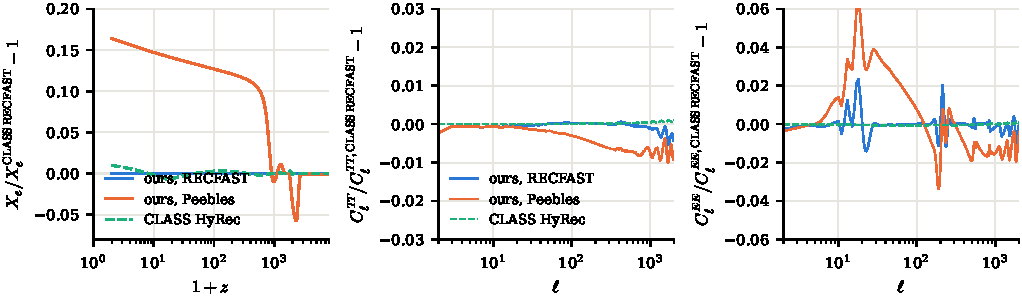
\includegraphics[width=\textwidth]{recfast}
\caption{\emph{Left:} $X_e(z)$ without reionization relative to CLASS run with RECFAST, for RECFAST (blue) and the
Peebles model (orange); dashed: CLASS with HyRec. \emph{Middle, right:} the unlensed TT and EE spectra relative to
CLASS with RECFAST. From the solver report.}
\label{fig:rec-recfast}
\end{figure}

\begin{validation}
\begin{itemize}
\item Plateaus: $X_e=1+2f_{\rm He}$ before helium recombination, $1+f_{\rm He}$ on the He$^+$ plateau; with $Y_p=0$ the
      helium solver reproduces the hydrogen-only code exactly.
\item $\int\gt\,\dd x=1$ to machine precision; $\tau'$, $\tau''$, $\gt'$, $\gt''$ against finite differences;
      $r_s$ against an independent quadrature; $T_b=T_\gamma$ early and $T_b\propto a^{-2}$ late.
\item The reionization optical depth agrees with the analytic integral for instantaneous reionization.
\item Against CLASS with RECFAST: $X_e$ to $3.3\times10^{-4}$ for $0\le z\le8000$ (both helium recombinations
      included), $z_*$ and $r_s(z_*)$ to $10^{-6}$ (\cref{fig:rec-recfast}). The rms difference of the unlensed TT
      from CLASS is $0.048\%$ for $30\le\ell\le1000$ with RECFAST against $0.64\%$ with the Peebles model.
\end{itemize}
\end{validation}

\begin{cppcode}[Recombination on its own]
#include <FML/Cosmology/Recombination/RecombinationHistory.h>
using namespace FML::COSMOLOGY;
CosmologyParameters params = CosmologyParameters::Planck2018Baseline();
BackgroundCosmology cosmo(params);
cosmo.solve();
RecombinationHistory rec(cosmo);
rec.solve();
rec.info();                               // z_*, r_s, z_drag, tau_reio, ...
double g = rec.g_tilde_of_x(-7.0);        // visibility at x = -7
rec.output("data/recombination.txt");
\end{cppcode}

\chapter{Linear perturbations}\label{ch:linear-perturbations}
\chapterstatus{written}{2026-11-14}

The primordial fluctuations are small, so their evolution until well after recombination follows from Einstein's
equations and the Boltzmann equations of every species expanded to first order around the background of
\cref{ch:background}. The background is translation invariant, so each Fourier mode evolves independently, and
isotropy means that only $k=|\vk|$ matters. This chapter gives the equations solved by the Einstein--Boltzmann solver,
the approximations that make them tractable, and the numerical methods; \cref{ch:cmb-spectra} turns the solution
into observables and \cref{ch:extended-models} describes the perturbations of the models beyond $\Lambda$CDM.

\begin{modulebox}{Cosmology/Perturbations}
Driver: \file{Perturbations.h/.cpp} (class \cls{Perturbations}, namespace \nsp{FML::COSMOLOGY}), \file{Tensors.h/.cpp},
\file{Isocurvature.h}.\par
Model library (namespace \nsp{FML::COSMOLOGY::PERTURBATIONS}, header-only): \file{PerturbationTypes.h},
\file{SpeciesPerturbation.h} and \file{SpeciesPerturbation_<name>.h}, \file{PerturbedFieldEquation.h} and
\file{PerturbedFieldEquation_<name>.h}, \file{QuasiStaticGravity*.h}, \file{PerturbationModel*.h}, \file{Presets.h}.\par
Documentation: \file{Cosmology/Perturbations/README.md}, \file{Cosmology/EinsteinBoltzmannSolver/README.md},
\file{DEVELOPING.md}, the report \file{report/paper.pdf} (Secs.~III, VIII).
\end{modulebox}

\section{Structure of the calculation}\label{sec:pert-structure}

The perturbation module is organised around the observation that photons and baryons, coupled by Thomson scattering,
need special treatment (tight coupling, the line-of-sight sources), while every other species only interacts with
the rest through gravity (or through an explicit coupling to one partner). The solver therefore has
\begin{itemize}
\item a fixed \emph{core}: the baryons $(\delta_b,v_b)$, the photon temperature multipoles $\Theta_0\ldots
      \Theta_{\ell_{\max}}$, the polarization multipoles $\Theta^P_0\ldots\Theta^P_{\ell_{\max}}$ and the potential
      $\Phi$;
\item one \emph{block} per perturbed species of the model (\cls{SpeciesPerturbation}): CDM, massless neutrinos,
      massive neutrinos, scalar fields, dark-energy fluids, and coupled pairs (CDM + dark energy) as one block. A block
      owns its variables, initial conditions, equations, approximation switches and outputs, and communicates with the
      rest only through its \emph{moments} --- $\delta\rho$, $\delta p$, the momentum flux $(\rho+p)\theta/k$ and the
      shear $(\rho+p)\sigma$ --- and the metric $(\Phi,\Psi,\Phi')$ it receives;
\item the \emph{perturbed field equations} of the theory of gravity (\cls{PerturbedFieldEquation}), which compute
      $\Psi$ and $\Phi'$ from the summed moments; scalar--tensor theories add their own variables here.
\end{itemize}
A \cls{PerturbationModel} says which background species get which perturbation block and which field equations to
use; the registry (\file{Presets.h}) builds the model for each name of \cref{tab:bg-models}. A species object is shared
by all modes and threads (no per-mode state). Smooth species ($\Lambda$, $w_0w_a$) get no perturbations.

\section{Metric and Einstein equations}

The scalar perturbations are evolved in the conformal Newtonian gauge with the conventions of
Dodelson \cite{Dodelson2003} and Callin \cite{Callin2006}:
\begin{equation}
\dd s^2=a^2(\eta)\left[-(1+2\Psi)c^2\dd\eta^2+(1+2\Phi)\gamma_{ij}\dd x^i\dd x^j\right],
\end{equation}
where $\gamma_{ij}$ is the spatial metric of curvature $K$. $\Psi$ is the Newtonian potential and $\Phi$ the curvature
perturbation; with this sign convention $\Psi=-\Phi$ without anisotropic stress (the ``Planck'' spatial potential is
$\Phi_P=-\Phi$). We write $\kappa\equiv ck/\Hp$ for the wavenumber in units of the Hubble scale. With all species
contributing through their moments, the $00$ (combined with $0i$) and the traceless $ij$ Einstein equations are
\begin{align}
\Phi'&=\Psi-\frac{c^2k^2}{3\Hp^2}\Phi+\frac{H_0^2a^2}{2\Hp^2}\sum_i\frac{\delta\rho_i}{\rho_{c0}},
\label{eq:pert-einstein1}\\
\Psi&=-\Phi-\frac{12H_0^2a^2}{c^2k^2}\sum_i\frac{(\rho_i+p_i)\sigma_i}{\rho_{c0}},
\label{eq:pert-einstein2}
\end{align}
where the shear moments are normalised so that the photons contribute $(\rho+p)\sigma\to\rho_{c0}\Om_\gamma a^{-4}
\Theta_2$, and in a curved universe $k^2$ is replaced by $k^2-3K$ in the $00$ equation (and in the Poisson equation for the
comoving density). For the standard species in a flat universe \cref{eq:pert-einstein1,eq:pert-einstein2} read
\begin{align}
\Phi'&=\Psi-\frac{\kappa^2}{3}\Phi+\frac{H_0^2}{2\Hp^2}\left[\frac{\Om_{\rm cdm}\delta_{\rm cdm}+\Om_b\delta_b}{a}
+\frac{4(\Om_\gamma\Theta_0+\Om_\nu\mathcal N_0)}{a^2}\right],\\
\Psi&=-\Phi-\frac{12H_0^2}{c^2k^2a^2}\left[\Om_\gamma\Theta_2+\Om_\nu\mathcal N_2\right].
\end{align}
$\Phi$ is evolved and $\Psi$ is algebraic; the Poisson and momentum constraints that are not integrated are used as
tests.

\section{Photons}

The photon distribution is a Planck spectrum with a direction-dependent temperature,
$f=[\exp(p/k_BT(1+\Theta))-1]^{-1}$, and $\Theta(k,\mu,x)$ depends on $\mu=\hat\vk\cdot\hat{\bm p}$. The linearised
Boltzmann equation is
\begin{equation}
\Theta'+i\kappa\mu\Theta=-\Phi'-i\kappa\mu\Psi-\tau'\left[\Theta_0-\Theta+i\mu v_b-\tfrac12P_2(\mu)\Pi\right],
\label{eq:pert-boltzmann}
\end{equation}
with free streaming, the redshift from the changing spatial curvature, the gravitational redshift and Thomson
scattering at the rate $-\tau'$ per unit $x$ (\cref{ch:recombination}), including the Doppler shift off moving
electrons and the angular dependence of the scattering, $\Pi=\Theta_2+\Theta^P_0+\Theta^P_2$. With the Legendre moments
$\Theta_\ell=\frac{1}{(-i)^\ell}\int_{-1}^1\frac{\dd\mu}{2}P_\ell(\mu)\Theta(\mu)$ --- $\delta_\gamma=4\Theta_0$,
$v_\gamma=-3\Theta_1$, and $\Theta_2$ the anisotropic stress --- the hierarchy is
\begin{align}
\Theta_0'&=-\kappa\Theta_1-\Phi',\\
\Theta_1'&=\frac\kappa3\left(\Theta_0-2s_2\Theta_2+\Psi\right)+\tau'\left(\Theta_1+\frac{v_b}{3}\right),\\
\Theta_\ell'&=\frac{\kappa}{2\ell+1}\left[\ell s_\ell\Theta_{\ell-1}-(\ell+1)s_{\ell+1}\Theta_{\ell+1}\right]
+\tau'\left(\Theta_\ell-\frac{\Pi}{10}\delta_{\ell2}\right),\qquad\ell\ge2,
\end{align}
and the polarization hierarchy \cite{Zaldarriaga1995}, which has no gravitational source,
\begin{equation}
\Theta^{P\prime}_\ell=\frac{\kappa}{2\ell+1}\left[\ell s_\ell\Theta^P_{\ell-1}-(\ell+1)s_{\ell+1}\Theta^P_{\ell+1}\right]
+\tau'\left[\Theta^P_\ell-\frac\Pi2\left(\delta_{\ell0}+\frac{\delta_{\ell2}}{5}\right)\right].
\end{equation}
The curvature factors $s_\ell=\sqrt{1-(\ell^2-1)K/k^2}$ are 1 in a flat universe (\cref{sec:pert-curvature}); with
\param{polarization} \code{= false} the polarization is dropped and $\Pi=\Theta_2$.

\paragraph*{Truncation.} The hierarchies are truncated at \param{lmax} (default 8) with the closure of Ma and
Bertschinger \cite{Ma1995}, which assumes the free-streaming solution $\Theta_\ell\propto j_\ell$ for the last
multipole and avoids reflecting power back to low $\ell$:
\begin{equation}
\Theta'_{\ell_{\max}}=\kappa s_{\ell_{\max}}\Theta_{\ell_{\max}-1}-\frac{c(\ell_{\max}+1)\cot_K(\eta)}{\Hp}\Theta_{\ell_{\max}}
+\tau'\Theta_{\ell_{\max}},
\end{equation}
with $\cot_K(\eta)=1/\eta$ when flat. Only the low multipoles enter the line-of-sight sources, so a small $\ell_{\max}$
suffices.

\section{Neutrinos}

\paragraph*{Massless neutrinos} obey the photon hierarchy without collisions, $\tau'=0$, with multipoles
$\mathcal N_\ell$, truncated at \param{lmax_nu} (default 22; 30 changes the spectra by $<5\times10^{-4}$, 12 gives
$0.35\%$ in $P(k)$ at $k=0.3\Mpc^{-1}$). Their quadrupole is a large anisotropic stress in the radiation era, when they
are $41\%$ of the radiation.

\paragraph*{Massive neutrinos.} A massive particle's velocity $cq/\epsilon$ depends on its momentum, so following
Ma and Bertschinger \cite{Ma1995} the distribution is written $f=f_0(q)[1+\Psi_\nu(\vk,\hat n,q,\eta)]$ and expanded
in Legendre multipoles $\Psi_\ell(q)$ at a set of momenta:
\begin{align}
\Psi_0'&=-\kappa\frac q\epsilon\Psi_1+\Phi'\frac{\dd\ln f_0}{\dd\ln q},\\
\Psi_1'&=\frac\kappa3\frac q\epsilon(\Psi_0-2\Psi_2)-\frac\kappa3\frac\epsilon q\Psi\frac{\dd\ln f_0}{\dd\ln q},\\
\Psi_\ell'&=\frac{\kappa}{2\ell+1}\frac q\epsilon\left[\ell\Psi_{\ell-1}-(\ell+1)\Psi_{\ell+1}\right],\qquad\ell\ge2,
\end{align}
with the moments
\begin{equation}
\delta\rho_\nu\propto\int\dd q\,q^2\epsilon f_0\Psi_0,\quad
(\rho+p)_\nu\theta_\nu\propto k\int\dd q\,q^3f_0\Psi_1,\quad
(\rho+p)_\nu\sigma_\nu\propto\frac23\int\dd q\,\frac{q^4}{\epsilon}f_0\Psi_2 .
\end{equation}
For $M\to0$ and $\Psi_\ell=-\mathcal N_\ell\,\dd\ln f_0/\dd\ln q$ this reduces to the massless system. The defaults are
\param{n_q_ncdm} $=8$ Gauss--Laguerre momenta and \param{lmax_ncdm} $=17$ (as CLASS; 16 momenta or $\ell_{\max}=25$
change $C_\ell$ and $P(k)$ by $<3\times10^{-5}$). Deep inside the horizon, $k\eta>$ \param{ncdm_fluid_trigger} $=31$,
the hierarchy is replaced by the fluid approximation of Lesgourgues and Tram \cite{LesgourguesTram2011} for
$\delta_\nu,\theta_\nu,\sigma_\nu$, with the adiabatic sound speed $c_a^2=\frac{w}{3(1+w)}(5-\mathfrak p/p)$ and a
viscosity closure for the shear, as in CLASS. This reduces the system from $\sim190$ to $\sim49$ variables and changes
$P(k)$ by up to $0.3\%$ at $m_\nu=0.3$\,eV, as CLASS's approximation does. Degenerate species are one hierarchy;
different masses (\param{m_nu_list}) each have their own, with outputs \code{delta_ncdm_<i>}, \code{v_ncdm_<i>} and the
totals \code{delta_ncdm}, \code{v_ncdm}.

\section{Cold dark matter and baryons}

CDM is collisionless and non-relativistic, and baryons exchange momentum with the photons:
\begin{align}
\delta_{\rm cdm}'&=\kappa v_{\rm cdm}-3\Phi', & v_{\rm cdm}'&=-v_{\rm cdm}-\kappa\Psi,\\
\delta_b'&=\kappa v_b-3\Phi', & v_b'&=-v_b-\kappa\Psi+\tau'R\,(3\Theta_1+v_b),
\end{align}
with $R=4\rho_\gamma/(3\rho_b)$ ensuring momentum conservation. (In a curved universe the continuity equations carry
the factor $(1-3K/k^2)$ on $\Phi'$ in the conventions of the code.)

\section{Initial conditions}\label{sec:pert-ic}

At \param{pert_x_start} $=-18$ every mode is far outside the horizon in the radiation era. For adiabatic
perturbations, normalised to a primordial comoving curvature perturbation $\mathcal R=1$ (the actual amplitude enters
through $\mathcal P_\mathcal R(k)$ in \cref{ch:cmb-spectra}),
\begin{gather}
\Psi=-\frac{1}{\frac32+\frac25f_\nu},\qquad \Phi=-\left(1+\frac25f_\nu\right)\Psi,\qquad
f_\nu=\frac{\rho_{\rm fs}}{\rho_\gamma+\rho_{\rm fs}},\\
\delta_{\rm cdm}=\delta_b=-\tfrac32\Psi,\quad v_{\rm cdm}=v_b=-\tfrac\kappa2\Psi,\quad
\Theta_0=\mathcal N_0=-\tfrac12\Psi,\quad \Theta_1=\mathcal N_1=\tfrac\kappa6\Psi,\\
\mathcal N_2=-\frac{(cka)^2\Phi}{12H_0^2\Om_\nu}\left(1+\frac{5}{2f_\nu}\right)^{-1},\qquad
\mathcal N_\ell=\frac{\kappa}{2\ell+1}\mathcal N_{\ell-1}\ (\ell\ge3),
\end{gather}
where $\rho_{\rm fs}$ is the density of the free-streaming species (all neutrinos). Each other species gives its
own adiabatic initial conditions. Isocurvature initial conditions are described in \cref{sec:cmb-isocurvature}.

\section{Tight coupling}\label{sec:pert-tc}

At early times $|\tau'|\gg1$ and the scattering terms make the system extremely stiff. The scattering locks
$\Theta_1\simeq-v_b/3$ and suppresses $\Theta_{\ell\ge2}$ by powers of $\kappa/\tau'$. In this regime only
$\delta_{\rm cdm}$, $v_{\rm cdm}$, $\delta_b$, $v_b$, $\Phi$, $\Theta_0$, $\Theta_1$ (and the other species) are evolved, and
\begin{gather}
\Theta_2=-\frac{8}{15}\frac{\kappa}{\tau'}\Theta_1\ \left(\tfrac{20}{45}\text{ without polarization}\right),\qquad
\Theta^P_0=\tfrac54\Theta_2,\qquad \Theta^P_2=\tfrac14\Theta_2,\\
\Theta_\ell=-\frac{\ell}{2\ell+1}\frac\kappa{\tau'}\Theta_{\ell-1}\quad(\ell\ge3).
\end{gather}
The baryon velocity and $\Theta_1$ follow from the second-order expansion of Callin \cite{Callin2006}, which
eliminates the large $\tau'$ terms in favour of the slip $q\equiv3\Theta_1'+v_b'$:
\begin{align}
q&=\frac{-[(1-R)\tau'+(1+R)\tau''](3\Theta_1+v_b)-\kappa\Psi+\left(1-\frac{\Hp'}{\Hp}\right)\kappa(-\Theta_0+2\Theta_2)
-\kappa\Theta_0'}{(1+R)\tau'+\frac{\Hp'}{\Hp}-1},\\
v_b'&=\frac{1}{1+R}\left[-v_b-\kappa\Psi+R\left(q+\kappa(-\Theta_0+2\Theta_2)-\kappa\Psi\right)\right],\qquad
\Theta_1'=\tfrac13(q-v_b').
\end{align}
Tight coupling ends at the first of $|\tau'|<$ \param{tc_tau_min} $=10$, $\kappa/|\tau'|>$ \param{tc_k_over_tau}
$=0.01$ (CLASS's $\tau_c/\tau_k$ trigger; $0.1$ left TT and EE $0.2$--$0.4\%$ low at $\ell=1000$--$2500$) and
$z=$ \param{tc_z_max} $=1700$; the full hierarchy is then initialised from the expressions above.

\paragraph*{Acoustic oscillations and diffusion damping.} At leading order in $1/\tau'$ the photon--baryon fluid is a
driven oscillator,
\begin{equation}
\frac{\dd}{\dd\eta}\left[(1+R_b)\dot\Theta_0\right]+\frac{c^2k^2}{3}\Theta_0=-\frac{c^2k^2}{3}(1+R_b)\Psi
-\frac{\dd}{\dd\eta}\left[(1+R_b)\dot\Phi\right],
\end{equation}
($R_b=1/R$, dots are $\dd/\dd\eta$) with the WKB solution $\Theta_0+(1+R_b)\Psi\simeq A\cos(kr_s)$. At next order
photon diffusion damps the oscillation as $e^{-k^2/k_D^2}$ \cite{HuSugiyama1995},
\begin{equation}
k_D^{-2}=\int_0^\eta\frac{c\,\dd\eta'}{6(1+R_b)n_e\sigma_Ta}\left[\frac{R_b^2}{1+R_b}+\frac{16}{15}\right].
\end{equation}
These analytic results, together with the superhorizon solution of Kodama and Sasaki \cite{Kodama1984}, the
radiation-era potential $\Phi=3\Phi_0(\sin y-y\cos y)/y^3$ ($y=k\eta/\sqrt3$), $\Phi=3/5$ in matter domination for
$\mathcal R=1$, and the growth rate $f\simeq\Om_m(x)^{0.55}$, are the tests of the module (\cref{fig:pert-tests}).

\section{Spatial curvature}\label{sec:pert-curvature}

In a curved universe the plane waves are replaced by eigenfunctions of the Laplacian, $\nabla^2G=-k^2G$, labelled by
$q^2=k^2+K$ and $\nu=q/\sqrt{|K|}$ \cite{HuSeljak1998,LesgourguesTram2014}. Open universes allow every $q>0$; closed
universes are finite and allow only integer $\nu\ge3$ for scalar modes. Three changes follow: $k^2\to k^2-3K$ in the
$00$ Einstein equation, the factors $s_\ell$ in all free-streaming couplings (for a closed universe $s_\nu=0$, so the
hierarchy of mode $\nu$ ends at $\ell=\nu-1$; the physical shear is $\Theta_2/s_2$), and $\cot_K(\eta)$ in the
truncation. The $k$-grid of the code is a grid in $q$; in a closed universe only integer $\nu$ are used, and in an open
universe the grid extends to $q=0.01\sqrt{|K|}$.

\section{Source functions}\label{sec:pert-sources}

After the evolution the temperature and $E$-mode source functions of the line-of-sight integration
(\cref{ch:cmb-spectra}) are built:
\begin{align}
S_T(k,x)&=\gt\left[\Theta_0+\Psi+\frac\Pi4\right]+e^{-\tau}(\Psi'-\Phi')-\frac{1}{ck}\frac{\dd}{\dd x}(\Hp\gt v_b)
+\frac{3}{4c^2k^2}\frac{\dd}{\dd x}\left[\Hp\frac{\dd}{\dd x}(\Hp\gt\Pi)\right],\label{eq:pert-ST}\\
S_E(k,x)&=\frac{3\gt\,\Pi}{4\,[k(\eta_0-\eta)]^2}.\label{eq:pert-SE}
\end{align}
The four terms of $S_T$ are the Sachs--Wolfe term (intrinsic temperature plus the redshift out of the potential at
last scattering), the integrated Sachs--Wolfe term, the Doppler term and the polarization/quadrupole correction. With
\param{store_source_components} they are stored separately (and \param{source_term} selects one for the
$C_\ell$). The derivatives come from integration by parts, which is valid only in a flat universe; in curved
universes the three parts $S_{T0}=\gt(\Theta_0+\Psi)+e^{-\tau}(\Psi'-\Phi')$, $S_{T1}=-\gt v_b$ and $S_{T2}=\gt\Pi/2$
are stored and projected with the radial functions and their derivatives (\cref{ch:cmb-spectra}). The numerator
$3\gt\Pi/4$ of $S_E$ is splined and the factor $1/[k(\eta_0-\eta)]^2$, which diverges today, applied on evaluation.

\begin{implementation}[Implementation: the perturbation solve]
\begin{itemize}
\item \emph{$k$-grid}: \param{pert_n_k} $=400$ modes logarithmically spaced in $[\code{pert_k_min},\code{pert_k_max}]=
      [5\times10^{-5},0.3]\Mpc^{-1}$; with \param{pert_dk_max} $>0$ a log-linear grid (the sources oscillate in $k$ with
      period $\sim2\pi/r_s$, so above $k\approx0.03\Mpc^{-1}$ a linear spacing of $0.004\Mpc^{-1}$ suffices: 112
      modes, the main saving of \code{precision = fast}).
\item \emph{$x$-grid of stored results}: \param{pert_n_x_early} $=300$ points in $[x_{\rm start},-8]$,
      \param{pert_n_x_recomb} $=1200$ in $[-8,-6]$ and \param{pert_n_x_late} $=600$ in $[-6,0]$.
\item \emph{Segments}: the integration is split into segments with fixed equations (tight coupling or not; each
      species' approximation scheme, e.g.\ the neutrino hierarchy or fluid; scalar-field switch points), each solved
      with its own method: \param{method_tc} (RK8PD) during tight coupling, \param{method_full} (GSL's implicit
      \code{msbdf} with a finite-difference Jacobian; $\sim30\times$ faster than RK at $k=0.3\Mpc^{-1}$) after it, and
      \param{method_ncdm} (explicit RK8PD) while the massive-neutrino hierarchy is active, where the dense linear algebra
      of BDF on $\sim190$ variables is $20\times$ slower. Tolerances \param{ode_relerr} $=10^{-8}$,
      \param{ode_abserr} $=10^{-10}$.
\item \emph{Parallelism}: the modes are solved in parallel with OpenMP.
\item \emph{Storage}: all outputs ($\delta_b$, $v_b$, $\Phi$, $\Psi$, $\Phi'$, $\Theta_\ell$, $\Theta^P_\ell$, $\Pi$,
      the species outputs by name, e.g.\ \code{get("delta_cdm", x, k)}, and the sources) are 2D bicubic splines in
      $(x,k)$.
\item \emph{Cost}: $\approx40$\,s for the fiducial model on two cores; massive neutrinos add $\approx7$\,s, curvature
      15--28\,s (mostly in the line of sight).
\end{itemize}
\end{implementation}

\begin{figure}[htbp]
\centering
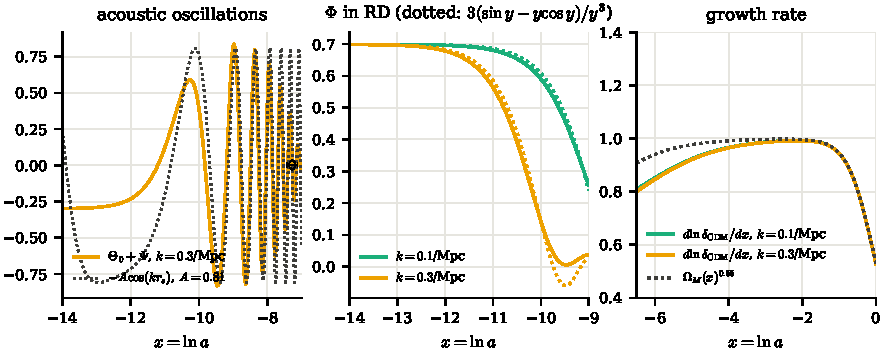
\includegraphics[width=\textwidth]{m3_tests}
\caption{Tests of the perturbations. \emph{Left:} $\Theta_0+\Psi$ for $k=0.3\Mpc^{-1}$ during the radiation era
against $-A\cos(kr_s)$ with the sound horizon of \cref{ch:recombination}. \emph{Middle:} $\Phi$ for modes entering in
radiation domination against the analytic radiation-era solution (dotted). \emph{Right:} the growth rate of
$\delta_{\rm cdm}$ against $\Om_m(x)^{0.55}$. From the solver report.}
\label{fig:pert-tests}
\end{figure}

\begin{figure}[htbp]
\centering
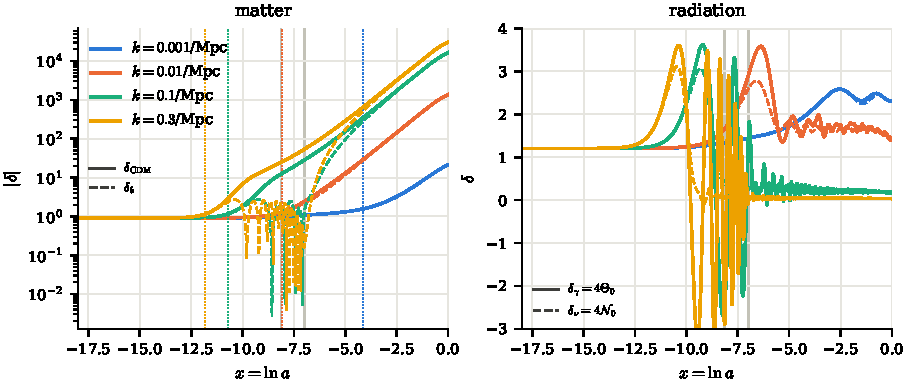
\includegraphics[width=\textwidth]{m3_delta}
\caption{Density perturbations for $k=0.001$, $0.01$, $0.1$ and $0.3\Mpc^{-1}$. \emph{Left:} $|\delta_{\rm cdm}|$
(solid) and $|\delta_b|$ (dashed). \emph{Right:} $\delta_\gamma=4\Theta_0$ (solid) and $\delta_\nu=4\mathcal N_0$
(dashed). Coloured dotted lines mark horizon entry, grey lines equality and decoupling. From the solver report.}
\label{fig:pert-delta}
\end{figure}

\begin{validation}
\begin{itemize}
\item Superhorizon evolution through equality against the Kodama--Sasaki solution; $\Phi\to3/5$ in matter
      domination; the radiation-era potential; the acoustic phase $\cos(kr_s)$; the growth rate $\Om_m^{0.55}$
      (\cref{fig:pert-tests}).
\item The Poisson and momentum constraints, continuity at the tight-coupling switch, free streaming of the neutrino
      multipoles; a nearly massless neutrino ($10^{-4}$\,eV) reproduces the massless one to $4\times10^{-7}$ in $\Phi$.
\item The model library equation by equation against the solver's former species classes ($10^{-8}$; $2\times10^{-7}$
      for the massive neutrinos), at $k=10^{-4},0.05,5\Mpc^{-1}$ and $x=-17,-8,-2,0$.
\item All perturbations against CLASS to $\sim0.1\%$; the end-to-end comparisons are in \cref{ch:cmb-spectra}.
\end{itemize}
\end{validation}

\begin{cppcode}[A custom model and the perturbations of a single mode]
#include <FML/Cosmology/Perturbations/Presets.h>
using namespace FML::COSMOLOGY::PERTURBATIONS;

FML::COSMOLOGY::BACKGROUND::BackgroundParameters p;
p.m_nu_eV = {0.06};
auto model   = make_perturbation_model("horndeski", p, {{"hd_cK", 1.0}, {"hd_cB", 0.6}, {"hd_cM", 0.3}});
auto ctx     = model->context();                       // settings: lmax_nu, lmax_ncdm, n_q_ncdm, ...
auto species = model->species_perturbations(ctx);      // CDM, massless and massive neutrinos
auto gravity = model->field_equation_perturbations(ctx);

// In the full solver (EinsteinBoltzmannSolver.h):
auto ebs = FML::COSMOLOGY::EinsteinBoltzmannSolver::from_file("params/planck2018.ini");
ebs.solve(FML::COSMOLOGY::EinsteinBoltzmannSolver::Stage::Perturbations);
double Phi = ebs.perturbations().get_Phi(-2.0, 0.1 / FML::UTILS::SI::Mpc);   // k in 1/m
\end{cppcode}

\chapter{CMB and matter power spectra}\label{ch:cmb-spectra}
\chapterstatus{written}{2026-11-14}

This chapter turns the source functions and transfer functions of \cref{ch:linear-perturbations} into observables:
the angular power spectra of the CMB temperature and polarization by line-of-sight integration, their lensing, the
contributions of tensor and isocurvature modes, the linear matter power spectrum, and real-space two-point functions.
It also describes the Einstein--Boltzmann solver as a program and a library.

\begin{modulebox}{Cosmology/Spectra and Cosmology/EinsteinBoltzmannSolver}
\file{Cosmology/Spectra}: \file{PowerSpectrum.h/.cpp} (class \cls{PowerSpectrum}: line of sight, $C_\ell$, $P(k)$),
\file{Lensing.cpp}, \file{HypersphericalBessel.cpp}, \file{TwoPoint.h/.cpp}, \file{PowerSpectrumTwoPoint.cpp},
\file{EisensteinHu.h}, \file{Halofit.cpp}, \file{PowerSpectrumReACT.cpp}, \file{NONLINEAR.md}.\par
\file{Cosmology/Perturbations}: \file{Tensors.h/.cpp}, \file{Isocurvature.h}.\par
\file{Cosmology/EinsteinBoltzmannSolver}: \file{EinsteinBoltzmannSolver.h/.cpp} (class
\cls{EinsteinBoltzmannSolver}), \file{Main.cpp} (the program \code{cmb}), \file{ParameterFile.h/.cpp},
\file{params/*.ini}, \file{README.md}, \file{OPTIONS.md}, \file{DEVELOPING.md}, \file{report/paper.pdf}.
\end{modulebox}

\section{Primordial spectra}

Every mode of \cref{ch:linear-perturbations} is normalised to $\mathcal R=1$, so every observable is a primordial
amplitude times a transfer function. The primordial curvature spectrum is
\begin{equation}
\mathcal P_\mathcal R(k)=A_s\left(\frac{k}{k_{\rm pivot}}\right)^{n_s-1+\frac12\alpha_s\ln(k/k_{\rm pivot})}
\end{equation}
(\param{A_s}, \param{n_s}, \param{alpha_s}, \param{k_pivot} $=0.05\Mpc^{-1}$), and the tensor spectrum
$\mathcal P_t=rA_s(k/k_{\rm pivot})^{n_t}$ with $n_t=-\frac r8\left(2-\frac r8-n_s\right)$ by default (the slow-roll
consistency relation, CLASS's \code{n_t = scc}; \param{n_t_consistency}, \param{n_t}).

\section{The line-of-sight integral}\label{sec:cmb-los}

Solving the photon hierarchy to $\ell\sim2500$ would require thousands of equations per mode. Seljak and Zaldarriaga
\cite{Seljak1996} noted that \cref{eq:pert-boltzmann} can be integrated formally along the photon path: with the
integrating factor $e^{ik\mu\eta-\tau}$, the Rayleigh expansion of the plane wave in spherical Bessel functions, and
integration by parts of the $\mu$-dependent terms,
\begin{equation}
\Theta_\ell(k)=\int_{-\infty}^0S_T(k,x)\,j_\ell[k(\eta_0-\eta)]\,\dd x,\qquad
\Theta^E_\ell(k)=\sqrt{\frac{(\ell+2)!}{(\ell-2)!}}\int_{-\infty}^0S_E(k,x)\,j_\ell[k(\eta_0-\eta)]\,\dd x,
\label{eq:cmb-los}
\end{equation}
with the sources of \cref{eq:pert-ST,eq:pert-SE}. This separates the physics (the sources, smooth in $k$ and needing
only low multipoles) from the geometry (the projection onto multipole $\ell$ at distance $\eta_0-\eta$). The angular
spectra are
\begin{equation}
C_\ell^{XY}=4\pi\int_0^\infty\frac{\dd k}{k}\,\mathcal P_\mathcal R(k)\,\Theta^X_\ell(k)\,\Theta^Y_\ell(k),\qquad
X,Y\in\{T,E\},
\label{eq:cmb-cl}
\end{equation}
reported as $D_\ell=\ell(\ell+1)C_\ell/2\pi$ in $\mu$K$^2$ (multiplied by $(10^6T_{\rm CMB})^2$). On large scales only
the Sachs--Wolfe term contributes and a scale-invariant spectrum gives the plateau $D_\ell\simeq A_sT_{\rm CMB}^2/25$;
the acoustic peaks sit at $\ell_n\approx n\ell_A-\phi_n$ with $\ell_A=\pi\chi_*/r_{s*}$, and diffusion damping
suppresses the power above $\ell_D=k_D\chi_*\approx2000$.

\begin{implementation}[Implementation: line of sight and $k$ integration]
\begin{itemize}
\item $j_\ell(z)$ is tabulated for all needed $\ell$ on a uniform grid with \param{bessel_points_per_2pi} $=32$
      points per $2\pi$ (and $j_\ell(z)/z^2$ for the $E$ source), for $O(1)$ lookups.
\item The $x$-integral (trapezoidal) starts at \param{x_start_los} $=-8.5$, where $e^{-\tau}$ makes the sources
      negligible; spacing \param{dx_recomb} $=0.003$ in $[\code{x_recomb_min},\code{x_recomb_max}]=[-7.6,-6.2]$ to
      resolve $\gt$, elsewhere uniform in $\eta$ with \param{n_eta_per_oscillation} $=5$ points per Bessel oscillation at
      $k_{\max}$.
\item The $k$-integral uses \param{n_k_per_oscillation} $=4$ points per period $2\pi/\eta_0$ of the transfer
      functions and $\Delta\ln k\le$ \param{dlnk_max} $=0.02$ at small $k$, over $[\code{los_k_min},\code{los_k_max}]$
      (default: the perturbation range). Do not set $k_{\max}$ much below $0.3\Mpc^{-1}$ for the $C_\ell$: $k_{\max}
      r_*>\ell$ is only a minimum.
\item $C_\ell$ is computed at a list of multipoles (\param{ells}, or every \param{ell_step} $=25$ above
      $\ell=100$, up to \param{ell_max}) and splined in $\ell$.
\item Doubling the line-of-sight and $k$ sampling changes the spectra by $<5\times10^{-5}$.
\end{itemize}
\end{implementation}

\subsection{Curved universes}

In a curved universe the projection uses the hyperspherical Bessel functions $\Phi^\nu_\ell(\chi)$ ($\chi$ in units of
the curvature radius), which solve
\begin{equation}
\Phi''+2\cot_K\chi\,\Phi'+\left[\nu^2-\mathrm{sgn}K-\frac{\ell(\ell+1)}{\sin_K^2\chi}\right]\Phi=0,
\end{equation}
with $\Phi^\nu_0=\sin(\nu\chi)/(\nu\sin_K\chi)$ and the recurrence
$\sqrt{\nu^2-\mathrm{sgn}K(\ell+1)^2}\,\Phi_{\ell+1}=(2\ell+1)\cot_K\chi\,\Phi_\ell-\sqrt{\nu^2-\mathrm{sgn}K\ell^2}\,
\Phi_{\ell-1}$; they reduce to $j_\ell(\nu\chi)$ for $\nu\to\infty$. The integration by parts of \cref{eq:pert-ST} is
not available, so the three parts of the source are projected separately \cite{LesgourguesTram2014}:
\begin{align}
\Theta_\ell(k)&=\int\dd x\left[S_{T0}\Phi_\ell+S_{T1}\frac{\sqrt{|K|}}{k}\Phi_\ell'
+S_{T2}\frac{3(|K|/k^2)\Phi_\ell''+\Phi_\ell}{2s_2}\right],\\
\Theta^E_\ell(k)&=\sqrt{\frac{(\ell+2)!}{(\ell-2)!}}\int\dd x\,\frac{3\gt\,\Pi}{4}\,\frac{\Phi_\ell}{s_2(kr)^2},
\end{align}
and in a closed universe the $k$-integral becomes a sum over integer $\nu$.

\begin{implementation}[Implementation: hyperspherical Bessel functions]
$\Phi^\nu_\ell$ is computed by upward recurrence below the turning point $\ell(\ell+1)=(\nu^2-\mathrm{sgn}K)\sin_K^2\chi$,
where it oscillates, and by Miller's downward recurrence above it \cite{Kosowsky1998,Tram2017} (starting exactly at
$\ell=\nu-1$ in a closed universe). For $\nu\ge$ \param{flat_approximation_nu} $=4000$ CLASS's flat approximation
replaces $\Phi^\nu_\ell$ by a rescaled $j_\ell$ with an amplitude correction ($\lesssim6\times10^{-4}$ in $C_\ell$ at
$\Om_k=\pm0.05$). The closed-universe sum uses a uniform integer stride in $\nu$ (rounding a uniform $k$ grid gave
irregular strides and 4\% errors). Modes with small $q$ use a proportionally coarser $x$-grid away from
recombination, never coarser than \param{dx_max_subsampled} $=0.01$. Tests: agreement with $j_\ell$ when flat to
$2\times10^{-12}$, the radial equation, the closed-form Gegenbauer functions to $10^{-13}$, and the $1/\nu^2$ approach
to $j_\ell$. \param{use_radial_functions} forces this path in a flat universe as a test (agreement with the
integrated-by-parts result to $5\times10^{-5}$).
\end{implementation}

\begin{figure}[htbp]
\centering
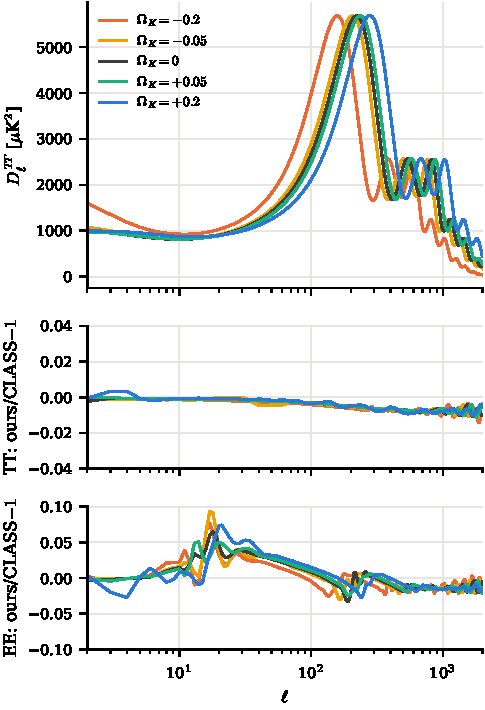
\includegraphics[width=0.6\textwidth]{curvature_spectra}
\caption{\emph{Top:} TT spectra for $\Omega_K=-0.2$, $-0.05$, 0, 0.05 and 0.2 at fixed matter and baryon density. \emph{Middle and bottom:} TT
and EE relative to CLASS with the same physics (unlensed). From the solver report.}
\label{fig:cmb-curvature}
\end{figure}


\section{The matter power spectrum}\label{sec:cmb-pk}

The matter power spectrum uses the comoving-gauge (synchronous-gauge, as CLASS) density contrast of the clustering
species,
\begin{equation}
\Delta_m(k,x)=\frac{\sum_i\rho_i\left[\delta_i-3(1+w_i)\Hp v_i/(ck)\right]}{\sum_i\rho_i},\qquad
P(k,x)=|\Delta_m(k,x)|^2\,\frac{2\pi^2}{k^3}\mathcal P_\mathcal R(k),
\end{equation}
summed over CDM, baryons and massive neutrinos for $P_m$ (and the ultralight axion when $m\ge10^{-25}$\,eV), and over
CDM and baryons for $P_{cb}$, the spectrum relevant for galaxy clustering in the presence of neutrinos. Inside the
horizon this is the Newtonian density contrast; it is consistent with the Poisson equation
$\Delta_m=\frac23\frac{c^2k^2}{\Hp^2}\frac{\Phi}{\Om_m(x)}$ up to radiation terms of order $10^{-3}$ on the largest
scales. $\sigma_R$ and $\sigma_8$ follow by integrating with the top-hat window; beyond the computed $k$-range $\Delta_m$
is extrapolated with the shape of the Eisenstein--Hu no-wiggle transfer function \cite{EisensteinHu1998} anchored at
$k_{\max}$ (\code{get_matter_power_spectrum_extrapolated}).

\paragraph*{Massive neutrinos} suppress $P_m$ below the free-streaming scale by $\approx-8f_\nu$ asymptotically
($f_\nu=\Om_\nu/\Om_m$): $2f_\nu$ from the non-clustering fraction and the rest from the slower growth
$\delta_{cb}\propto a^{1-3f_\nu/5}$ \cite{HuEisensteinTegmark1998,LesgourguesPastor2006}. The code reproduces CLASS's
suppression (16.1\% against 16.2\% at $k=0.5\hMpc$ for $m_\nu=0.3$\,eV; \cref{fig:cmb-neutrinos}).

\paragraph*{Nonlinear power.} \param{nonlinear} selects a nonlinear prescription (\code{halofit},
\code{halofit_bird}, \code{hmcode2016}, \code{hmcode2020}, \code{react}, \code{ee2}, \code{jbd_boost},
\code{axionhmcode}), added as a column of the output and used for the nonlinear lensing potential (the Weyl
potential of the Limber part is scaled by $\sqrt{P_{\rm NL}/P_{\rm L}}$). The methods are described in
\cref{ch:halo-model,ch:fitting-emulators}.

\begin{figure}[htbp]
\centering
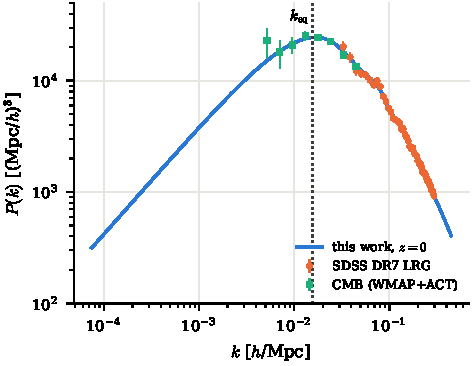
\includegraphics[width=0.6\textwidth]{m4_Pk}
\caption{The linear matter power spectrum today compared with the SDSS DR7 luminous red galaxy power spectrum \cite{Reid2010} and an estimate
from WMAP and ACT CMB data; the dotted line marks $k_{\rm eq}$. From the solver report.}
\label{fig:cmb-pk}
\end{figure}


\section{CMB lensing}\label{sec:cmb-lensing}

The CMB photons are deflected by the intervening structure: the observed temperature in direction $\hat{\bm n}$ is the
unlensed one at $\hat{\bm n}+\nabla\phi$, with the lensing potential
\begin{equation}
\phi(\hat{\bm n})=-\int_0^{\chi_*}\dd\chi\,\frac{\sin_K(\chi_*-\chi)}{\sin_K(\chi_*)\sin_K(\chi)}
\left(\Psi-\Phi\right)(\chi\hat{\bm n},\eta_0-\chi),
\end{equation}
the projection of the Weyl potential that bends light, with the last-scattering surface treated as one source plane
at the peak of $\gt$. $C_\ell^{\phi\phi}$ is computed with the line-of-sight machinery below \param{lensing_limber_ell}
$=30$ and with the Limber approximation above,
\begin{equation}
C_\ell^{\phi\phi}\simeq\int\dd\chi\,\frac{W^2(\chi)}{\sin_K^2\chi}\,
P_{\Psi-\Phi}\!\left(\frac{\ell+\frac12}{\sin_K\chi},\chi\right),
\end{equation}
with the Weyl potential extrapolated beyond $k_{\max}$ as $\ln k/k^2$; the two agree to $0.2\%$ for $40\le\ell\le200$.
The lensed spectra use the full-sky correlation-function method of Challinor and Lewis \cite{Challinor2005}, as in
CLASS: the lensed correlation functions are the unlensed ones with the deflection averaged, e.g.
\begin{equation}
\tilde\xi(\beta)=\sum_\ell\frac{2\ell+1}{4\pi}C_\ell\,e^{-\ell(\ell+1)\sigma^2(\beta)/2}d^\ell_{00}(\beta)+\ldots,
\end{equation}
where $\sigma^2(\beta)$ is the variance of the relative deflection of two points at separation $\beta$ and the dots
are terms of first and second order in the anisotropic part $C_{{\rm gl},2}(\beta)$. Polarization uses $\xi_\pm$ and
$\xi_\times$ with the Wigner functions $d^\ell_{22}$, $d^\ell_{2-2}$, $d^\ell_{20}$ (three-term recurrences). The lensed
spectra follow by Gauss--Legendre integration over $\cos\beta$. Lensing couples multipoles over
$\Delta\ell\sim$ hundreds, so the unlensed spectra are computed to $\ell_{\max}+$ \param{lensing_delta_ell}
(default $\max(500,\ell_{\max}/3)$). Lensing smooths the peaks (+3.4\% at the trough at $\ell=1000$), transfers power
to the damping tail and converts $E$ into $B$ modes ($D_\ell^{BB}$ peaks at $\approx0.09\muK$ near $\ell\approx900$).
Enable it with \param{lensing} \code{= true}.

\begin{figure}[htbp]
\centering
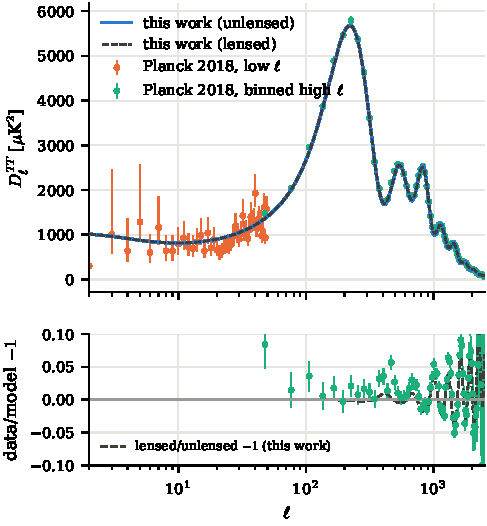
\includegraphics[width=0.49\textwidth]{m4_TT_planck}\hfill
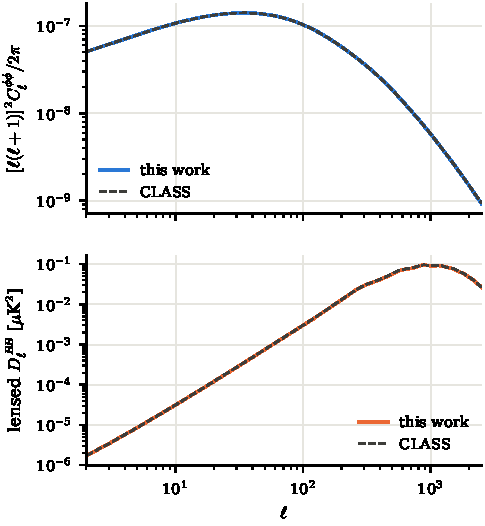
\includegraphics[width=0.49\textwidth]{m4_lensing}
\caption{\emph{Left:} unlensed and lensed TT spectra of the fiducial model compared with the Planck 2018 data
\cite{Planck2018spectra}, and the residuals. \emph{Right:} the lensing potential and the lensing $B$ modes against
CLASS (dashed). From the solver report, computed with the Peebles recombination model.}
\label{fig:cmb-tt}
\end{figure}

\begin{figure}[htbp]
\centering
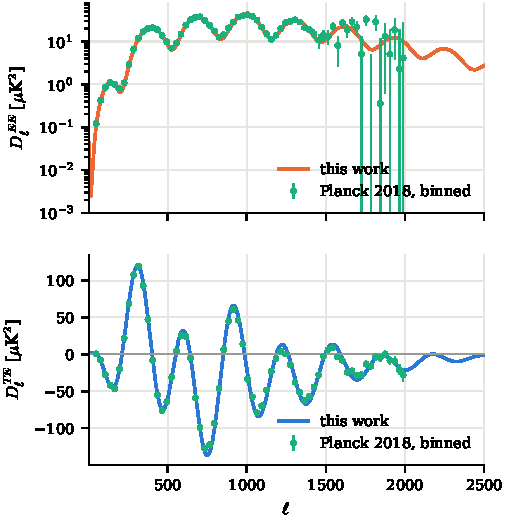
\includegraphics[width=0.49\textwidth]{m4_EE_TE}\hfill
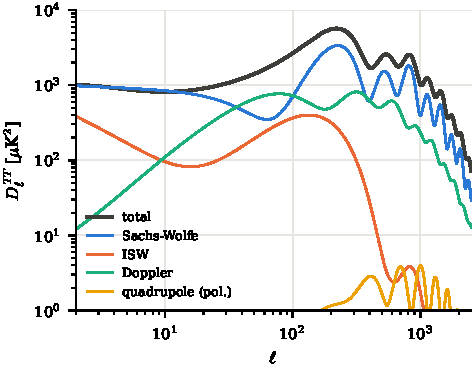
\includegraphics[width=0.49\textwidth]{m4_TT_components}
\caption{\emph{Left:} $E$-mode polarisation and the temperature--polarisation cross spectrum compared with binned Planck 2018 data.
\emph{Right:} the contributions to TT from the four terms of the temperature source function (Sachs--Wolfe, ISW, Doppler, polarisation),
each computed alone; they add in amplitude, not in power. From the solver report (Peebles recombination).}
\label{fig:cmb-ee-te}
\end{figure}


\section{Tensor modes}\label{sec:cmb-tensors}

With \param{r} $>0$ the solver adds primordial gravitational waves. The tensor perturbation $h$ obeys
\begin{equation}
\ddot h+(2+\alpha_M)\Hp\dot h+c^2k^2h=\frac{16\pi Ga^2}{M_*^2}\,\Pi_T
\end{equation}
(dots: conformal time), sourced by the tensor anisotropic stress $\Pi_T$ of photons and neutrinos, with the friction
$\alpha_M$ and the effective Planck mass $M_*^2$ of the theory of gravity (Horndeski $\alpha_M$, Brans--Dicke $\phi$,
$f(R)$ $1+f_R$; GR otherwise). The photon temperature and polarization and the neutrino tensor hierarchies are those
of CLASS (flat), with tight coupling; massive neutrinos are evolved with the massless hierarchy and weighted by
$3p_{\rm ncdm}$ in the stress (CLASS's \code{tensor_method = massless}). Tensor TT, EE, TE are added to the scalar
spectra, BB is the tensor one, and all are lensed together. Settings: \param{tensor_k_max}, \param{tensor_dk_max},
\param{tensor_k_fine}, \param{tensor_n_k_per_oscillation}, \param{tensor_lmax}, \param{tensor_lmax_nu},
\param{tensor_neutrinos}, \param{tensor_ell_max} $=600$. Flat universes only; about 10\,s on two cores.

\begin{validation}[Validation: tensors]
\begin{itemize}
\item Against CLASS ($r=0.1$): unlensed tensor TT, EE, BB to 0.1--0.5\% for $\ell\le300$; lensed total BB to
      $0.1\%$ for $\ell=50$--300.
\item The damping of the amplitude by neutrino free streaming: $\times0.8026$ (Weinberg's value \cite{Weinberg2004}).
\item Matter era without stress: $h=3j_1(k\eta)/(k\eta)$ to $0.2\%$; Horndeski $c_M=0.5$: $h\propto1/(aM_*)$ to $10^{-3}$.
\end{itemize}
\end{validation}

\section{Isocurvature modes}\label{sec:cmb-isocurvature}

The CDM, baryon, neutrino density and neutrino velocity isocurvature modes (\param{f_cdi}, \param{f_bi},
\param{f_nid}, \param{f_niv}, with tilts \code{n_*} and correlations \code{c_ad_*} with the adiabatic mode, in
CLASS's conventions) have $P_{II}=f^2A_s(k/k_{\rm pivot})^{n_I-1}$ and $P_{\mathcal RI}=c\sqrt{P_{\mathcal R\mathcal R}
P_{II}}$; the isocurvature modes are uncorrelated with each other and $\sum c^2<1$. Their superhorizon initial
conditions are CLASS's series \cite{BucherMoodleyTurok2000}. The correlation matrix is Cholesky-factored into
independent components, each one perturbation solve with a mixture of adiabatic and isocurvature initial conditions
and one line-of-sight pass, and the $C_\ell$, $C_\ell^{\phi\phi}$ and $P(k)$ are summed over the components. For
\code{model = axion}, \param{f_axi} is the density isocurvature of the axion, or \param{ax_log10_Hinf} sets it from
the field fluctuation $\delta\phi=H_{\rm inf}/2\pi$: $f_{\rm axi}^2A_s=H_{\rm inf}^2/(\pi^2\phi_i^2)$,
$n_{\rm axi}=1-r/8$. Isocurvature modes require GR and the standard species. Against CLASS the pure CDI and NID modes
agree to $5\times10^{-4}$ in TT and EE for $10\le\ell\le600$.

\section{Two-point functions}\label{sec:cmb-twopoint}

\paragraph*{CMB correlation functions.} For a statistically isotropic sky
$C(\theta)=\sum_\ell\frac{2\ell+1}{4\pi}C_\ell B_\ell^2P_\ell(\cos\theta)$, with an optional Gaussian beam
$B_\ell=e^{-\ell(\ell+1)\sigma_b^2/2}$ (\param{cmb_correlation_beam_fwhm}); for polarization
$\xi_\pm=\sum_\ell\frac{2\ell+1}{4\pi}(C_\ell^{EE}\pm C_\ell^{BB})d^\ell_{2,\pm2}$ and
$\xi_X=\sum_\ell\frac{2\ell+1}{4\pi}C_\ell^{TE}d^\ell_{20}$ \cite{Challinor2005}.

\paragraph*{Matter correlation function.} $\xi(r)=\frac{1}{2\pi^2r}\int_0^\infty\dd k\,kP(k)\sin(kr)$ is computed with
Filon's method \cite{Filon1929} ($kP(k)$ linear between tabulated points, the product with $\sin kr$ integrated
analytically), so the grid only needs to resolve $P(k)$ and its BAO wiggles. The BAO peak appears at
$r\approx100\Mpch$; $\sigma_8$ agrees with CLASS to $4\times10^{-5}$.

\paragraph*{Projected density.} For a tracer with redshift distribution $n(z)$ (Gaussian, \param{angular_z},
\param{angular_sigma_z}) and linear bias \param{angular_bias},
\begin{equation}
C_\ell=4\pi\int\frac{\dd k}{k}\mathcal P_\mathcal R(k)\Delta_\ell(k)^2,\qquad
\Delta_\ell(k)=\int\dd\chi\,W(\chi)\,b\,\Delta_m(k,\chi)\,j_\ell(k\chi),
\end{equation}
exactly below $\ell=200$ and with the Limber approximation \cite{Limber1953,LoVerde2008}
$C_\ell=\int\dd\chi\,W^2b^2P((\ell+\frac12)/\chi,\chi)/\chi^2$ above; $w(\theta)$ follows from the Legendre sum. Only
the density term is included (no RSD, magnification or relativistic terms). These agree with CLASS's number-count
spectra to $2\times10^{-3}$.

\begin{figure}[htbp]
\centering
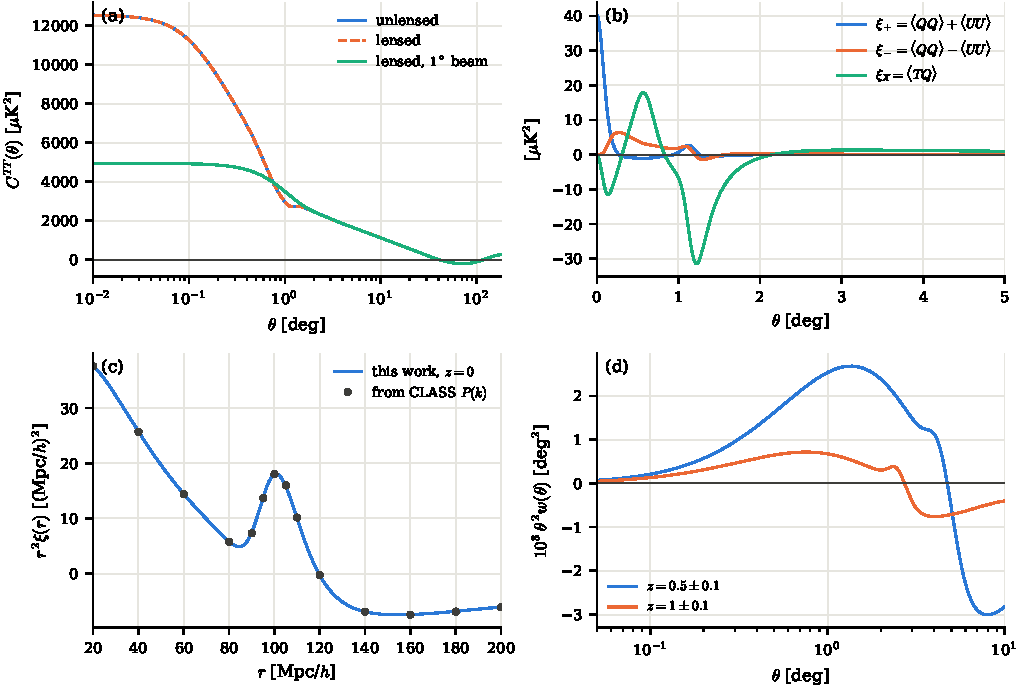
\includegraphics[width=0.85\textwidth]{twopoint}
\caption{Two-point functions of the fiducial model: (a) the CMB temperature correlation function, unlensed, lensed and with a $1^\circ$ beam;
(b) the polarisation correlation functions; (c) the matter correlation function today with the BAO peak, against the transform of CLASS's
$P(k)$; (d) the angular correlation function of matter projected over Gaussian redshift distributions ($\sigma_z=0.1$, $b=1$). From the
solver report.}
\label{fig:cmb-twopoint}
\end{figure}


\section{The solver as a program and a library}\label{sec:cmb-solver}

\paragraph*{Program.} \code{make} in \file{Cosmology/EinsteinBoltzmannSolver} builds \code{./cmb}:
\begin{paramfile}[Running the solver]
./cmb                                              # the fiducial model
./cmb params/planck2018.ini                        # parameters from a file
./cmb m_nu=0.06 lensing=true output_dir=data/test  # command-line values override the file
./cmb --write-defaults my.ini                      # every parameter with its default and description
\end{paramfile}
Every cosmological, precision and output parameter can be set in a file (\code{name = value}, \code{\#} comments) or
on the command line; unknown names are errors. \param{preset} \code{= planck2018} or \code{planck2018_baseline} loads a
parameter set; \param{precision} \code{= fast} sets precision parameters tuned for CMB likelihoods (lensed TT, EE, TE to
$\ell=2500$ in 13--16\,s instead of $\sim70$\,s, $\Delta\chi^2\approx0.2$ for Planck-like noise). The outputs are
\file{background.txt}, \file{recombination.txt}, \file{perturbations_k<k>.txt}, \file{cells.txt} ($D_\ell^{TT,EE,TE}$
in $\mu$K$^2$), \file{cells_lensed.txt}, \file{matter_power.txt} ($k$ in $\hMpc$, $P_m$, $P_{cb}$, $P_{\rm NL}$,
$P_{\rm axion}$), \file{transfer.txt}, and optionally the correlation functions and angular spectra; each run also
writes \file{params_used.ini}.

\paragraph*{Library.}
\begin{cppcode}[The solver from code]
#include <FML/Cosmology/EinsteinBoltzmannSolver/EinsteinBoltzmannSolver.h>
using namespace FML::COSMOLOGY;

auto ebs = EinsteinBoltzmannSolver::from_file("params/planck2018.ini", {"lensing=true"});
ebs.solve();                                      // or solve(Stage::Perturbations)
const auto & ps = ebs.power_spectrum();
double sigma8 = ps.get_sigma8();
double DTT    = ps.get_Dell_TT_lensed(1000);      // muK^2
double Pk     = ps.get_matter_power_spectrum(0.0, 0.1 / FML::UTILS::SI::Mpc);  // x = 0, k in 1/m
ebs.output();                                     // the files enabled in the settings
\end{cppcode}
The solver is also used by SimulationCode for its initial conditions (\code{ic_type_of_input = internal},
\cref{ch:growth-transfer}) and as the theory code of CosmologyFitting (\cref{ch:sampling-fitting}).

\begin{figure}[htbp]
\centering
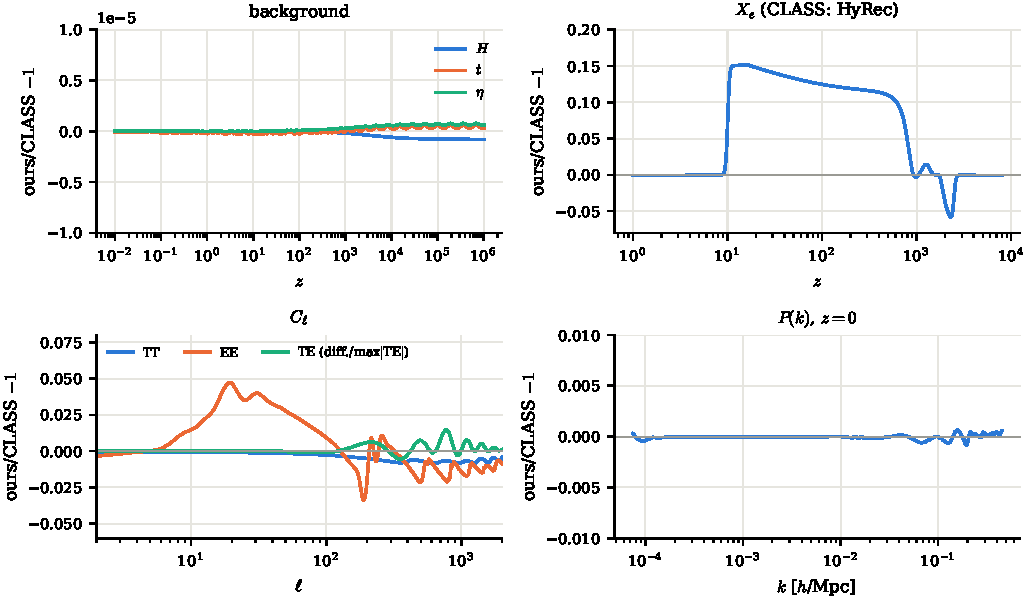
\includegraphics[width=\textwidth]{validation_class}
\caption{Comparison of the solver with CLASS run with the same physics: background, recombination, the unlensed and
lensed CMB spectra and $P(k)$. From the solver report.}
\label{fig:cmb-validation}
\end{figure}

\begin{figure}[htbp]
\centering
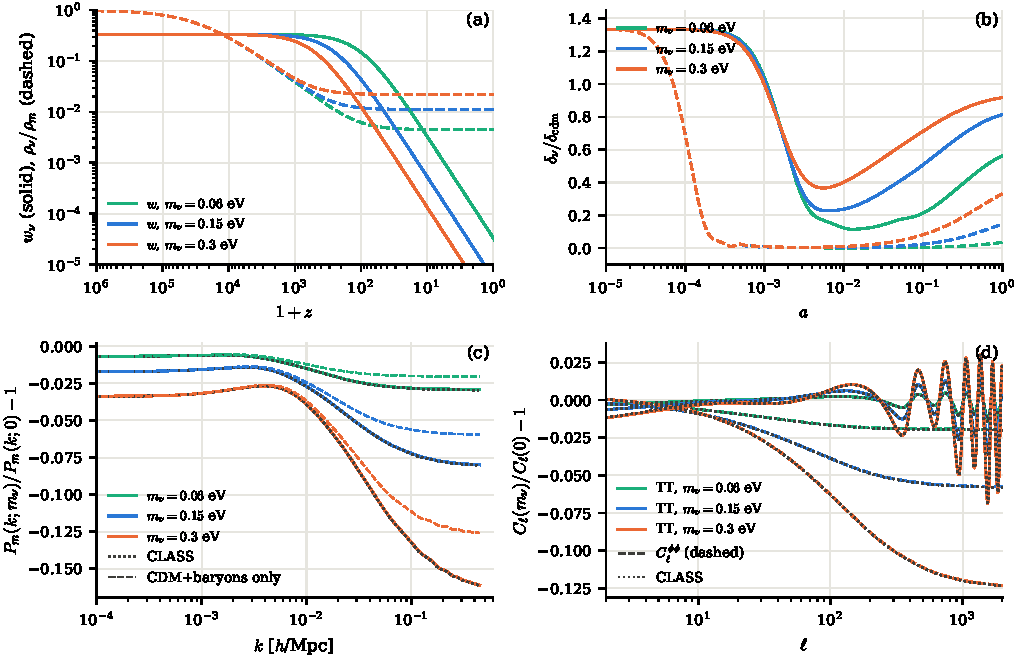
\includegraphics[width=\textwidth]{neutrinos}
\caption{Massive neutrinos with $m_\nu=0.06$, $0.15$ and $0.3$\,eV at fixed $h$, $\omega_b$, $\omega_{\rm cdm}$: the
equation of state, $\delta_\nu/\delta_{\rm cdm}$, the change of $P_m$ and $P_{cb}$, and of TT and
$C_\ell^{\phi\phi}$, with CLASS (dotted). From the solver report.}
\label{fig:cmb-neutrinos}
\end{figure}

\begin{validation}[Validation: the solver against CLASS (same physics, RECFAST)]
\begin{center}\small
\begin{tabular}{@{}ll@{}}
\toprule
Quantity & Agreement \\
\midrule
Background ($H$, $t$, $\eta$) & $10^{-7}$ \\
$X_e$ ($0\le z\le8000$) & $3\times10^{-4}$ \\
$z_*$, $r_s(z_*)$ & $10^{-6}$ \\
TT (rms, $30\le\ell\le1000$; $1000<\ell\le2000$) & $5\times10^{-4}$; $3\times10^{-3}$ \\
EE (rms) & $2\times10^{-3}$ \\
$P(k)$ & $10^{-3}$ \\
Lensed/unlensed TT ratio & $10^{-3}$ \\
Effect of the neutrino mass on TT, $C_\ell^{\phi\phi}$, $P_m$ & $5\times10^{-4}$ \\
$\sigma_8$ & $4\times10^{-5}$ \\
Curved models $|\Om_k|\le0.2$ & as flat; first peak to $\pm1$ in $\ell$ \\
Projected $C_\ell$ and $w(\theta)$ & $2\times10^{-3}$ \\
\bottomrule
\end{tabular}
\end{center}
The Peebles recombination model gives TT to 0.6--0.8\% and EE to 1.4\% rms. The figures and the scripts that
reproduce these numbers are in \file{report/} and \file{python/}.
\end{validation}

\chapter{Dark energy and modified gravity in linear theory}\label{ch:extended-models}
\chapterstatus{written}{2026-11-17}

The Einstein--Boltzmann solver has a library of some twenty models beyond $\Lambda$CDM. Their backgrounds were
described in \cref{ch:background}; this chapter gives their perturbations. Every model uses the conventions of
\cref{ch:linear-perturbations} (Newtonian gauge, $x=\ln a$, $\Phi$ with the sign of Callin; below
$\Phi_P=-\Phi$ is the potential with the Planck sign) and is selected by \code{model = <name>} with its parameters in
the parameter file. The quasi-static limits of the theories, collected in \cls{QuasiStaticGravity}, are shared with the
growth factors, the one-loop hybrid bias and SimulationCode.

\begin{modulebox}{Cosmology/Perturbations (models)}
Species: \file{SpeciesPerturbation_ScalarField.h} (quintessence, EDE, axion), \file{_DarkEnergyFluid.h} (dark
scattering, IDE), \file{_CoupledQuintessence.h}, \file{_MassiveNeutrinos.h}, \file{_CDM.h},
\file{_MasslessNeutrinos.h}.\par
Field equations: \file{PerturbedFieldEquation_GeneralRelativity.h}, \file{_BransDicke.h}, \file{_MuSigma.h} (with
DGP and Hu--Sawicky), \file{_HorndeskiAlpha.h}, \file{_CubicGalileon.h}.\par
Quasi-static theories: \file{QuasiStaticGravity.h} and \file{QuasiStaticGravity_<name>.h} (MuSigma, HuSawicky,
DGP, BransDicke, Symmetron, Dilaton, MBeta, CubicGalileon, Horndeski).\par
Models and registry: \file{PerturbationModel_<name>.h}, \file{PerturbationModel_HorndeskiTable.h}, \file{Presets.h}.
Validation: \file{EinsteinBoltzmannSolver/DEVELOPING.md}, report Sec.~XI.
\end{modulebox}

\section{Quasi-static gravity}\label{sec:ext-quasistatic}

Far inside the horizon and neglecting time derivatives of the extra fields, a theory of gravity modifies the Poisson
equations for the comoving density $\rho\Delta$ of all species:
\begin{equation}
k^2\Psi=-4\pi Ga^2\,\mu(k,a)\,\rho\Delta,\qquad k^2(\Phi_P+\Psi)=-8\pi Ga^2\,\Sigma(k,a)\,\rho\Delta .
\label{eq:ext-musigma}
\end{equation}
$\mu=G_{\rm eff}/G$ is the force on non-relativistic matter (growth, $N$-body forces) and $\Sigma$ the lensing (Weyl)
potential; GR is $\mu=\Sigma=1$. \cls{QuasiStaticGravity} gives, on any \cls{Background},
\begin{itemize}
\item \code{mu_sigma(x, k)}: $\mu$, $\Sigma$ and $\dd(2\Sigma-\mu)/\dd x$ at fixed $k$ (needed by the solver);
\item \code{second_order_source(x, k)}: the $D_1^2$ source of the 2LPT growth equation relative to GR,
      $D_2''+(2+\frac{\dd\ln H}{\dd x})D_2'=\frac32\Om_m(a)\mu\,(D_2-s_2D_1^2)$ ($s_2=1$ in GR and in theories without a
      nonlinear term; smaller with Vainshtein screening);
\item \code{screening()}: the type (Newtonian potential for chameleon-like theories, density for Vainshtein, gradient
      for k-mouflage) and the surviving fraction of the fifth force as a function of that quantity, used by the
      approximate screening methods of SimulationCode (\cref{ch:mg-simulations}).
\end{itemize}
$k$ is in units of $H_0/c$ (\code{koverH0}). The theories are summarised in \cref{tab:ext-qs}.

\begin{table}[htbp]
\centering\small
\caption{Quasi-static theories. $\beta$ and $m$ are the coupling and mass of a scalar fifth force; screening factors
are $\min(1,\epsilon\,\Phi_{\rm crit}/|\Phi_N|)$ for potential screening, with an efficiency $\epsilon$.}
\label{tab:ext-qs}
\begin{tabularx}{\textwidth}{@{}lXX@{}}
\toprule
Theory & $\mu(k,a)$, $\Sigma$ & Screening \\
\midrule
$\mu$--$\Sigma$ (Planck/DES) & $\mu=1+\mu_0\frac{\Om_{\rm DE}(a)}{\Om_{\rm DE,0}}$, $\Sigma=1+\Sigma_0\frac{\Om_{\rm DE}(a)}{\Om_{\rm DE,0}}$ & --- \\
Hu--Sawicky $f(R)$ & $\frac{1+\frac13\frac{k^2}{k^2+a^2m^2}}{1+f_R}$, $\Sigma=\frac{1}{1+f_R}$ & potential, $\Phi_{\rm crit}=\frac32|f_R(a)|$ \\
DGP & $1+\frac{1}{3\beta}$, $\beta=1-2\epsilon\frac{Hr_c}{c}\left(1+\frac{\dd\ln H}{3\dd\ln a}\right)$, $\Sigma=1$ & Vainshtein (density) \\
Cubic Galileon & $\mu=\Sigma=1+\frac{\Om_\phi(a)}{1-2\frac{\dd\ln H}{\dd\ln a}-\Om_\phi(a)}$ & Vainshtein (density) \\
Brans--Dicke & from the sub-horizon field equations, $G_{\rm eff}=G\phi_*/\phi$ & --- \\
Symmetron & $1+\frac{2\beta^2(a)k^2}{k^2+a^2m^2(a)}$ after $a_{\rm ssb}$, $\Sigma=1$ & potential \\
Dilaton & as symmetron with $m=m_0a^{-r}$, $\beta=\beta_0e^{s(a^p-1)/p}$ & potential, $\Phi_{\rm crit}=1/(2A_2)$ \\
$(m,\beta)$ & as symmetron with $\beta=\beta_0a^{n_\beta}$, $m=m_0a^{n_m}$ & potential \\
Horndeski (table) & from the $\alpha$'s of the reduced theory \cite{Kimura2012} & Vainshtein \\
\bottomrule
\end{tabularx}
\end{table}

\paragraph*{Hu--Sawicky $f(R)$} \cite{HuSawicki2007}. In the high-curvature regime $f_R=-|f_{R0}|(R_0/R)^{n+1}$ and
$f_{RR}=-(n+1)f_R/R$, with the background Ricci scalar $Rc^2/(3H_0^2)=2E^2(2+\dd\ln E/\dd x)-2\Om_ke^{-2x}$ (the
$\order{f_{R0}}$ corrections to the expansion are neglected, as in MGCAMB). The scalaron mass is
$m^2c^2/H_0^2=(1+f_R)\,Rc^2/[3H_0^2(n+1)|f_R|]$, and $Q=(k/a)^2f_{RR}/(1+f_R)=(k/a)^2/(3m^2)$ gives the familiar
$\mu=(1+4Q)/[(1+3Q)(1+f_R)]$: gravity is enhanced by $4/3$ below the Compton wavelength $1/m$.

\paragraph*{DGP} \cite{KoyamaMaartens2006}. The brane-bending mode strengthens gravity on the normal branch
($\epsilon=-1$) and weakens it on the self-accelerating branch; it does not change the lensing potential. $H(a)$ is
that of the background, whichever it is. The nonlinear term of the field equation gives
$s_2=1-2(r_cH_0/c)^2\rho_m(a)/(9\beta^3\mu)$. For a spherical top-hat the fifth force is reduced by
$2(\sqrt{1+e}-1)/e$ with $e=8(r_cH_0/c)^2\rho_m\delta/(9\beta^2)$; the screening approximation used by default replaces
$\rho_m(a)$ by $\Om_m$ and $\delta$ by $1+\delta$, which reproduces the exact multigrid $P(k)$ better (0.5\% against
1.2\% rms at $z=0$).

\paragraph*{Cubic Galileon.} On the tracker the quasi-static scalar equation is that of DGP's brane-bending mode
with a time-dependent crossover scale, $\beta=(1-2\varepsilon-\Om_\phi(a))/(3\Om_\phi(a))$ and
$(r_cH_0/c)^2=E^2/(2\Om_\phi(a)\Om_{\phi0})$, $\varepsilon=\dd\ln H/\dd\ln a$ \cite{Barreira2013}; the Galileon enters
$\Phi$ and $\Psi$ alike, so $\Sigma=\mu$ ($\mu=1.77$ today for $\Om_{\phi0}=0.68$). In voids ($e<-1$) there is no real
solution and $e=-1$ is used, as in the multigrid solver.

\paragraph*{Symmetron, dilaton and $(m,\beta)$} \cite{Brax2012}. These chameleon-like theories have a scalar of mass
$m(a)$ coupled to matter with strength $\beta(a)$ and $\mu=1+2\beta^2k^2/(k^2+a^2m^2)$. The symmetron
\cite{Brax2012}, generalised to the powers $(N,M)$ (even, $M>N\ge2$; $(2,4)$ is the original) with
$V\propto-\frac1N(\phi/\phi_*)^N+\frac1M(\phi/\phi_*)^M$, has no fifth force before symmetry breaking at $a_{\rm ssb}$ and
\begin{equation}
\chi=\frac{\phi}{\phi_*}=\left[1-(a_{\rm ssb}/a)^3\right]^{\frac{1}{M-N}},\quad \beta(a)=\beta\chi^{N-1},\quad
m^2=\frac{\chi^{N-2}\left[1-(a_{\rm ssb}/a)^3\right]}{(H_0L/c)^2}\frac{H_0^2}{c^2},
\end{equation}
with the vacuum range $L$ (\param{sym_assb}, \param{sym_beta}, \param{sym_L_mpch}, \param{sym_N}, \param{sym_M}). The
environment-dependent dilaton has $A(\phi)=1+A_2\phi^2/(2\Mpl^2)$, $m=m_0a^{-r}$ ($r\le3/2$) and
$\beta(a)=\beta_0\exp[s(a^p-1)/p]$ with $p=2r-3$, $s=9\Om_mA_2\xi^2$, $\xi=H_0/m_0$ (\param{dil_A2},
\param{dil_beta0}, \param{dil_r}, \param{dil_xi}). The $(m,\beta)$ parameterisation uses power laws
(\param{mb_beta0}, \param{mb_n_beta}, \param{mb_m0}, \param{mb_n_m}); its screening threshold
$\Phi_{\rm crit}=\phi(a)/(2\beta\Mpl)$ needs the background field $\phi/\Mpl=9\Om_m\int_0^a\beta/(a'^3(m/H_0)^2)\,
\dd\ln a'$.

\paragraph*{In the Einstein--Boltzmann solver} the quasi-static theories (\code{musigma}, \code{dgp}, \code{fr},
\code{symmetron}, \code{dilaton}, \code{mbeta}) use the $\mu$--$\Sigma$ field equations. On super-horizon scales
$\rho\Delta\sim(k/\Hp)^2\delta\rho$, so computing the potentials directly from \cref{eq:ext-musigma} would lose all
precision there. Instead the GR potential of the comoving density, $\Phi_{\rm GR}=\frac32H_0^2a^2\rho\Delta/
(\rho_{c0}c^2k^2)$, is evolved with the equation that follows from energy--momentum conservation of all species
(with $A=3/(2c^2k^2)$ and densities times $H_0^2a^2$),
\begin{multline}
\Phi_{\rm GR}'\left[1+3A(\rho+p)(2\Sigma-\mu)\right]=-\Phi_{\rm GR}+A\Big[-\frac{ck}{\Hp}\,{\rm flux}
+3\left(\frac{\Hp'}{\Hp}-1\right)\frac{\rm flux}{ck/\Hp}-2\,{\rm shear}\\+3(\rho+p)\Psi-3(\rho+p)(2\Sigma-\mu)'\Phi_{\rm GR}\Big],
\end{multline}
and $\Psi=-\mu\Phi_{\rm GR}-S$, $\Phi=(2\Sigma-\mu)\Phi_{\rm GR}$ with $S$ the anisotropic stress term. The GR energy
constraint minus its momentum-constraint form is added, so $\mu=\Sigma=1$ is exactly the GR code. These models require
a flat universe and $2\Sigma-\mu\ge0$.

\section{Scalar fields: quintessence, early dark energy and axions}\label{sec:ext-scalar}

The field perturbation $\delta\phi$ obeys the Klein--Gordon equation in Newtonian gauge. With
$w\equiv\delta\phi_x-\phi_x\Psi$, which removes $\Psi'$,
\begin{align}
\delta\phi_x&=w+\phi_x\Psi,\\
w_x&=-\left(2+\frac{\Hp'}{\Hp}\right)w-\left(\frac{ck}{\Hp}\right)^2\delta\phi-\frac{3v_{\phi\phi}}{E^2}\delta\phi
-3\phi_x\Phi'-\frac{3v_\phi}{E^2}\Psi,
\end{align}
with the moments (times $H_0^2a^2/\rho_{c0}$) $\delta\rho=\Hp^2\phi_xw/3+H_0^2a^2v_\phi\delta\phi$,
$\delta p=\Hp^2\phi_xw/3-H_0^2a^2v_\phi\delta\phi$, flux $=(ck/\Hp)\Hp^2\phi_x\delta\phi/3$ and no anisotropic stress.
The frozen field starts with $\delta\phi=w=0$.

\paragraph*{The oscillating field as a fluid.} When the background replaces a fast-oscillating field by a fluid
(\cref{sec:bg-scalar-fields}), the perturbations switch at the same $x$ to the effective fluid of an oscillating
field \cite{Poulin2018}, with $w=c_a^2=w_{\rm osc}$ and the rest-frame sound speed
\begin{equation}
c_s^2(k,x)=\frac{2(n-1)W+(ck/\Hp)^2}{2(n+1)W+(ck/\Hp)^2},\qquad W=(\varpi/H)^2,
\end{equation}
for $V\propto|\phi-\phi_{\min}|^{2n}$ ($n=1$: the ultralight axion, $c_s^2=k^2/(k^2+4m^2a^2)$), where $\varpi$ is the
angular frequency of the oscillation, computed from the period of the actual potential at the switch and scaled as
$\rho^{(n-1)/2n}$ afterwards. The fluid obeys the dark-energy fluid equations below. At the switch $(\delta\phi,w)$ is
split into a shift along the trajectory, which carries the momentum, and a change of amplitude; the density is set
from the comoving density perturbation, which is continuous and does not oscillate, so the Einstein constraints hold
exactly through the switch (the neglected terms are $\order{H/m}<10^{-2}$ of the field's perturbation). For the axion
with \param{ax_switch_mH} $\le4$ the switch keeps axionCAMB's synchronous-gauge $\delta$ and $(1+w)v$ continuous.

\section{Dark-energy fluids and dark-sector interactions}\label{sec:ext-fluids}

A dark-energy fluid of constant $w$ and rest-frame sound speed $\hat c_s^2$ (variables $\delta_{\rm DE}$ and
$u=\theta/(ck)$) obeys
\begin{align}
\delta_{\rm DE}'&=-(1+w)\left(\frac{ck}{\Hp}u+3\Phi'\right)-3(\hat c_s^2-w)\left[\delta_{\rm DE}+\frac{3(1+w)u}{ck/\Hp}\right],\\
u'&=-(1-3\hat c_s^2)u+\frac{ck}{\Hp}\left[\frac{\hat c_s^2\delta_{\rm DE}}{1+w}+\Psi\right],
\end{align}
with $\delta p_{\rm DE}=\rho_{\rm DE}[\hat c_s^2\delta_{\rm DE}+3(1+w)(\hat c_s^2-w)u/(ck/\Hp)]$. It is evolved in one block
with the CDM it interacts with.

\paragraph*{Dark scattering} \cite{Simpson2010,BaldiSimpson2015} exchanges only momentum:
\begin{gather}
v_c'=-v_c-\frac{ck}{\Hp}\Psi+\frac{\Gamma_c}{\Hp}(v_{\rm DE}-v_c),\qquad u'=\ldots-\frac{\Gamma_{\rm DE}}{\Hp}(u-u_c),\\
\Gamma_{\rm DE}=ac\,\xi\rho_c,\qquad \Gamma_c=(1+w)\frac{\rho_{\rm DE}}{\rho_c}\Gamma_{\rm DE}.
\end{gather}
While $\Gamma_{\rm DE}/\Hp>200$ the dark-energy velocity is locked to that of the dark matter (its momentum is negligible
then). The covariant dark Thomson-like scattering has $\Gamma_c=\alpha H_0a^4/\Om_{c0}$. Parameters: \param{ds_w},
\param{ds_xi}, \param{ds_cs2}; $\xi=0$ is $w$CDM with dark-energy perturbations.

\paragraph*{Interacting dark energy} \cite{Valiviita2008} transfers energy along the dark-matter four-velocity, with
the perturbed rate from the local expansion of the dark matter, $\delta Q/Q=\delta_{\rm DE}-\Psi+E$,
$E=-\frac13\frac{ck}{\Hp}v_c+\Phi'$, and the doom factor $d=\xi/[3(1+w)]$:
\begin{align}
\delta_c'&=\frac{ck}{\Hp}v_c-3\Phi'+\xi\frac{\rho_{\rm DE}}{\rho_c}(\delta_{\rm DE}-\delta_c+E),\qquad v_c'=-v_c-\frac{ck}{\Hp}\Psi,\\
\delta_{\rm DE}'&=-(1+w)\left(\frac{ck}{\Hp}u+3\Phi'\right)-3(\hat c_s^2-w)\left[\delta_{\rm DE}+\frac{3(1+w)(1+d)u}{ck/\Hp}\right]-\xi E,\\
u'&=\left[3\hat c_s^2-1+3d(\hat c_s^2-w)\right]u+\frac{ck}{\Hp}\left[\frac{\hat c_s^2\delta_{\rm DE}}{1+w}+\Psi\right]+\xi u+3dv_c .
\end{align}
The early-time instability \cite{Valiviita2008} is avoided for $d<0$; the code rejects $d>0$ (\param{ide_stability_check})
and backgrounds with $\rho_c<0$ before today.

\paragraph*{Coupled quintessence} \cite{Wetterich1995,Amendola2000} evolves the CDM and the field in one block:
\begin{align}
\delta_c'&=\frac{ck}{\Hp}v_c-3\Phi'-\beta\,\delta\phi_x,\qquad
v_c'=-(1-\beta\phi_x)v_c-\frac{ck}{\Hp}\Psi+\beta\frac{ck}{\Hp}\delta\phi,\\
w'&=\ldots-\frac{3(v_\phi-\beta\rho_c)}{E^2}\Psi+\frac{3\beta\rho_c}{E^2}\delta_c,
\end{align}
i.e.\ a fifth force that makes the effective gravitational constant of the dark matter $G(1+2\beta^2)$ on small
scales, and a drag $\propto\beta\phi_xv_c$. The Fading Dark Sector \cite{ObiedVafaWu2026} (\code{fading_dark_sector},
\cref{sec:bg-coupledquintessence}) uses these perturbations with $\lambda=c$, $\beta=c'$; its quasi-static limit
$G_{\rm eff,\chi\chi}=G[1+2c'^2k^2/(k^2+a^2m_{\rm eff}^2)]$ is the $k\gg am_{\rm eff}$ limit $1+2\beta^2$ here, since
$m_{\rm eff}\sim H$.

\section{Scalar--tensor theories with full perturbations}\label{sec:ext-scalartensor}

\paragraph*{Brans--Dicke.} The perturbations ($\Phi$, $\delta\phi$, $\delta\phi'$) are evolved in full (derived
symbolically), with the background of \cref{sec:bg-bransdicke}; \code{quasi_static()} gives their sub-horizon limit.

\paragraph*{Cubic Galileon.} The braided scalar perturbations of the tracker are evolved in full, derived covariantly
and checked with the identity $\nabla^\mu T_{\mu\nu}=(\nabla\cdot J)\phi_\nu$.

\paragraph*{Horndeski in the $\alpha$ basis.} Following Bellini and Sawicki \cite{Bellini2014} and hi\_class
\cite{Zumalacarregui2017}, the linear theory is described by the kineticity $\alpha_K$, the braiding $\alpha_B$, the
running of the Planck mass $\alpha_M=\dd\ln M_*^2/\dd\ln a$ and the background; $\alpha_T=0$ (GW170817). The
Newtonian-gauge equations were derived for $L=F(\phi)R/2+G_2(\phi,X)-G_3(\phi,X)\Box\phi$, which realises any
$(\alpha_K,\alpha_B,\alpha_M)$, the $G_i$ eliminated with the definitions of the $\alpha$'s and the background
equations, and the system reduced to first order in $v=-\delta\phi/\phi'$ and $u=v'+\Psi$. The no-ghost and gradient
stability conditions
\begin{equation}
D=\alpha_K+\tfrac32\alpha_B^2>0,\qquad
Dc_s^2=(2-\alpha_B)\left[\frac{\alpha_B}{2}+\alpha_M-\frac{\dot H}{H^2}\right]-\frac{\rho_m+p_m}{H^2M_*^2}+\frac{\dot\alpha_B}{H}>0
\end{equation}
and a stiffness bound $c_s^2\le10^5$ are checked (\param{hd_stability_check}). The parameterisations are those of
hi\_class, $\alpha_X=c_X f(a)$ with $f=\Om_{\rm DE}(a)$, $a$ or 1 (\param{hd_parametrization}, \param{hd_cK},
\param{hd_cB}, \param{hd_cM}, \param{hd_M2_ini}), on a $\Lambda$CDM or $w_0w_a$ expansion (\param{hd_w0},
\param{hd_wa}); $\alpha_K=\alpha_B=0$ with $\alpha_M\neq0$ is rejected. \code{horndeski_table} uses the $\alpha$'s of a
reduced Horndeski theory given by its Lagrangian (\cref{ch:background}); the cubic Galileon built this way reproduces
\code{cubic_galileon} to $2\times10^{-5}$ in $P(k)$.

\section{Model summary and validation}

\begin{table}[htbp]
\centering\small
\caption{The models beyond $\Lambda$CDM, the parameters used for \cref{fig:ext-models}, their perturbations and
validation, and $\sigma_8$ and $P(k=0.1\hMpc)$ relative to $\Lambda$CDM with the same primordial spectrum,
$\Om_b$, $\Om_c$ and $h$ (from the solver report).}
\label{tab:ext-models}
\begin{tabularx}{\textwidth}{@{}llXlcc@{}}
\toprule
Model & Parameters & Perturbations & Main validation & $\frac{\sigma_8}{\sigma_8^{\Lambda}}$ & $\frac{P}{P^{\Lambda}}$ \\
\midrule
quintessence & $\lambda=1$ & full field & constraints, background & 0.978 & 0.956 \\
coupled quint. & $\lambda=0.5$, $\beta=0.05$ & field + CDM & constraints, growth & 1.037 & 1.071 \\
dark scattering & $w=-0.9$, $\xi=10$\,b/GeV & fluid + CDM & CLASS ($\xi=0$), drag & 0.962 & 0.925 \\
EDE & $f_{\rm EDE}=0.12$, $z_c=3630$ & full field & CLASS\_EDE & 0.945 & 0.899 \\
IDE & $\xi=-0.1$, $w=-0.95$ & fluid + CDM & constraints, $w$CDM limit & 1.124 & 1.254 \\
$\mu$--$\Sigma$ & $\mu_0=0.3$, $\Sigma_0=0.1$ & $\mu$--$\Sigma$ & growth equation & 1.038 & 1.077 \\
nDGP & $H_0r_c/c=1$, $\Lambda$CDM bg. & quasi-static & growth equation & 1.070 & 1.145 \\
sDGP & $\Om_\Lambda=0$ & quasi-static & growth equation & 0.809 & 0.654 \\
Brans--Dicke & $\omega=100$ & full field & constraints, $G_{\rm eff}$ & 1.043 & 1.093 \\
$f(R)$ & $|f_{R0}|=10^{-5}$, $n=1$ & quasi-static & scale-dep.\ growth & 1.073 & 1.066 \\
cubic Galileon & --- & full (braiding) & constraints, $G_{\rm eff}$ & 1.097 & 1.203 \\
Horndeski & $c_K=1$, $c_B=0.6$, $c_M=0.3$ & full ($\alpha$ basis) & hi\_class, 3 theories & 1.020 & 1.040 \\
\bottomrule
\end{tabularx}
\end{table}

\begin{figure}[htbp]
\centering
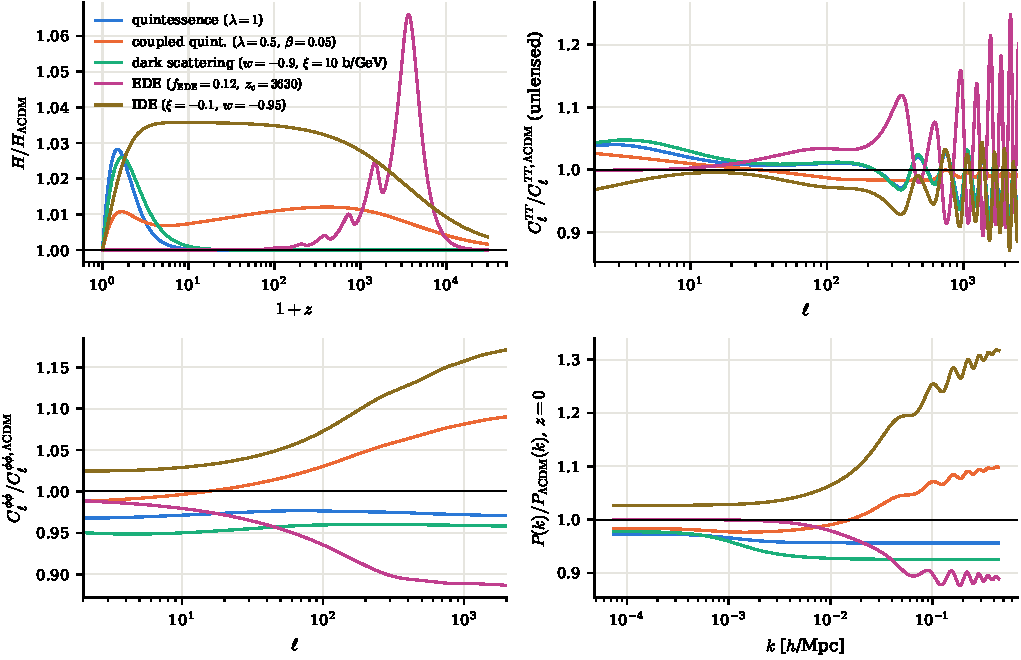
\includegraphics[width=\textwidth]{models_de}\\[2mm]
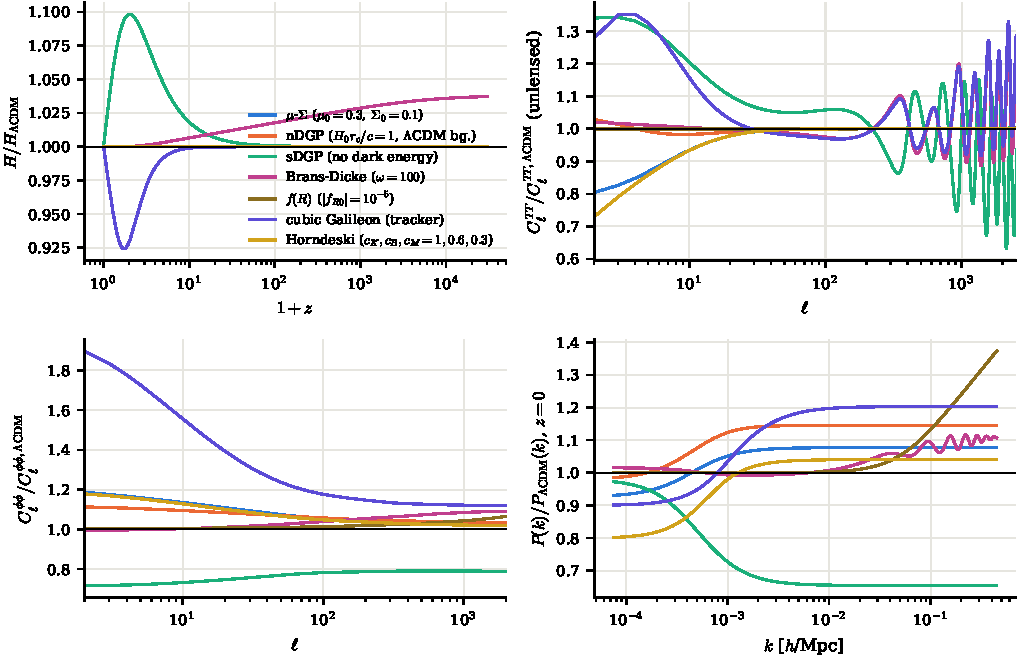
\includegraphics[width=\textwidth]{models_mg}
\caption{Dark-energy and dark-sector models (\emph{top}) and modified-gravity models (\emph{bottom}) relative to
$\Lambda$CDM: expansion rate, unlensed TT, lensing potential and $P(k)$ today, for the parameters of
\cref{tab:ext-models}. From the solver report.}
\label{fig:ext-models}
\end{figure}

\begin{validation}
Every model is tested in its GR/$\Lambda$CDM limit and, where possible, with the Einstein constraints that are not
integrated (momentum constraint to $10^{-8}$--$10^{-6}$; in interacting models the constraint holds only if the
exchange cancels between the species), with independent solutions of the quasi-static growth equation
($10^{-4}$--$7\times10^{-5}$), and against external codes: CLASS's fluid dark energy ($w$CDM, $P(k)$ to
$5\times10^{-5}$), CLASS\_EDE (ratios to $\Lambda$CDM to $3\times10^{-5}$ in $P(k)$ at $k\le0.05\hMpc$ and $10^{-3}$ in
TT), hi\_class (ratios to $10^{-4}$ in $P(k)$, $8\times10^{-4}$ in TT) and axionCAMB (axion isocurvature transfer to
$3\times10^{-3}$). The Horndeski $\alpha$ implementation reproduces the dedicated cubic Galileon ($5\times10^{-9}$),
quintessence ($2\times10^{-11}$) and Brans--Dicke ($9\times10^{-9}$) implementations. Details:
\file{EinsteinBoltzmannSolver/DEVELOPING.md}.
\end{validation}

\begin{paramfile}[Running a model]
./cmb params/fr.ini                                    # Hu-Sawicky f(R) (pert_k_max = 1, los_k_max = 0.3)
./cmb model=horndeski hd_cK=1 hd_cB=0.6 hd_cM=0.3 lensing=true
./cmb model=ede ede_fEDE=0.12 ede_log10zc=3.56 ede_theta_i=2.83
\end{paramfile}

\chapter{Growth factors, transfer functions and linear input}\label{ch:growth-transfer}
\chapterstatus{written}{2026-11-14}

Initial conditions for simulations, the time stepping of COLA and LPT, and many analytic predictions need two things
from linear theory: the growth factors of Lagrangian perturbation theory as functions of time (and of scale when
gravity or the matter content makes growth scale dependent), and the transfer functions of each species at the
initial time, in the right gauge. This chapter describes the one growth solver of the library and the transfer
providers that read CAMB and CLASS output or run the Einstein--Boltzmann solver of
\cref{ch:background,ch:recombination,ch:linear-perturbations}.

\begin{modulebox}{Cosmology/Growth}
\file{Cosmology/Growth/LPTGrowthFactors.h} (namespace \nsp{FML::COSMOLOGY::GROWTH}; header-only): \cls{LPTGrowthEquations},
\cls{LPTGrowthSettings}, \cls{LPTGrowthFactors}, \code{radiation_matter_growing_mode}. Used by SimulationCode's
\code{GravityModel} and by \code{LPT::compute_LPT_growth_factors_LCDM}/\code{_GeffGLCDM}; \code{history()} gives a
\cls{GrowthHistory} (\file{LPT/GrowthHistory.h}) for the $N$-body time stepping.\par
Documentation: \file{Cosmology/Growth/README.md}. Tests: \file{Cosmology/Growth/tests/test_growth.cpp}.
\end{modulebox}
\begin{modulebox}{TransferProviders and InitialConditions}
\file{InitialConditions/TransferProvider.h} (the interface: species, gauges, units, coverage),
\file{InitialConditions/InternalTransferProvider.h}, \file{LinearInput.h}, \file{SpeciesIC.h};
\file{TransferProviders/MakeTransferProvider.h}, \file{TabulatedTransferProvider.h},
\file{CAMBFileTransferProvider.h}, \file{CLASSTransferProvider.h}, \file{GaugeView.h}, \file{TransferTablesFile.h};
scripts \file{TransferProviders/scripts/make_class_transfer_tables.py},
\file{SimulationCode/scripts/make_camb_transfer_tables.py}.\par
Documentation: \file{TransferProviders/README.md}, \file{InitialConditions/README.md},
\file{SimulationCode/INITIAL_CONDITIONS.md}. Tests: \file{TransferProviders/tests}, \file{tests/test_transfers.cpp},
\file{tests/test_camb.cpp}, \file{Cosmology/EinsteinBoltzmannSolver/tests/test_transfer_provider.cpp}.
\end{modulebox}

\section{Linear growth of structure}\label{sec:growth-linear}

Inside the horizon and after the radiation era, the clustering matter (CDM and baryons, or all matter) behaves as a
pressureless fluid with
\begin{equation}
\dot\delta+\frac1a\nabla\cdot[(1+\delta)\bm v]=0,\qquad
\dot{\bm v}+H\bm v+\frac1a(\bm v\cdot\nabla)\bm v=-\frac1a\nabla\Psi,\qquad
\nabla^2\Psi=4\pi Ga^2\mu\,\bar\rho_m\delta,
\end{equation}
with a possibly scale- and time-dependent effective gravitational constant $\mu=G_{\rm eff}/G$
(\cref{sec:ext-quasistatic}). Linearising and changing to $x=\ln a$ with $'=\dd/\dd x$ gives the linear growth
equation for $\delta(\vk,a)=D_1(k,a)\delta(\vk,a_{\rm ini})/D_1(k,a_{\rm ini})$,
\begin{equation}
D_1''+\left(2+\frac{\dd\ln E}{\dd x}\right)D_1'=\frac32\Om_m(x)\,\mu(k,x)\,D_1,
\label{eq:growth-D1}
\end{equation}
where $\Om_m(x)=\rho_m(x)/(\rho_{c0}E^2)$. In Einstein--de Sitter ($\Om_m=1$, $\dd\ln E/\dd x=-3/2$, $\mu=1$) the
growing mode is $D_1\propto a$; in $\Lambda$CDM the growth slows when $\Lambda$ dominates and
$f\equiv\dd\ln D_1/\dd x\simeq\Om_m(x)^{0.55}$.

\subsection{Higher orders in Lagrangian perturbation theory}

In LPT the particle positions are $\vx=\vq+\bm\Psi(\vq,t)$, expanded as
$\bm\Psi=\bm\Psi^{(1)}+\bm\Psi^{(2)}+\bm\Psi^{(3)}+\ldots$ with each order a product of a growth factor and a spatial
field \cite{Bouchet1995}: $\nabla_q\cdot\bm\Psi^{(1)}=-D_1\delta_{\rm ini}$, $\nabla_q\cdot\bm\Psi^{(2)}=
\frac{D_2}{2}\sum_{i\ne j}(\phi^{(1)}_{,ii}\phi^{(1)}_{,jj}-\phi^{(1)2}_{,ij})$, and the third-order terms $D_{3a}$ (the
determinant of the Hessian of $\phi^{(1)}$) and $D_{3b}$ (the mixed first--second-order term); the spatial
kernels are described in \cref{ch:lpt}. The growth factors obey (with $S\equiv\frac32\Om_m(x)\mu(k,x)$)
\begin{align}
D_1''+\left(2+\tfrac{\dd\ln E}{\dd x}\right)D_1'&=S\,s_1\,D_1,\label{eq:growth-orders}\\
D_2''+\left(2+\tfrac{\dd\ln E}{\dd x}\right)D_2'&=S\,s_2\,(D_2-N\,D_1^2),\nonumber\\
D_{3a}''+\left(2+\tfrac{\dd\ln E}{\dd x}\right)D_{3a}'&=S\,s_{3a}\,(D_{3a}-2D_1^3),\nonumber\\
D_{3b}''+\left(2+\tfrac{\dd\ln E}{\dd x}\right)D_{3b}'&=S\,s_{3b}\,(D_{3b}+D_1^3-D_2D_1).\nonumber
\end{align}
In EdS the growing solutions are
\begin{equation}
D_2=-\tfrac37D_1^2,\qquad D_{3a}=-\tfrac13D_1^3,\qquad D_{3b}=\tfrac{5}{21}D_1^3 .
\end{equation}
The factors in \cref{eq:growth-orders} generalise GR:
\begin{itemize}
\item $N(x,k)$ is the \emph{second-order source} of the theory of gravity (\code{second_order_source} of
      \cls{QuasiStaticGravity}): 1 in GR and in theories whose scalar field equation has no nonlinear term; smaller
      than 1 for DGP and the cubic Galileon, whose Vainshtein term already acts at second order.
\item $s_i(x,k)$ are per-order source factors (default 1). With massive neutrinos the CDM+baryon fluid feels the
      gravity of only the clustering part of the matter; with $\rho_m$ including the neutrinos one uses e.g.\
      $s_1=1-f_\nu$ above the free-streaming scale, or the source computed from the neutrino transfer functions
      (as SimulationCode does).
\item A velocity friction $\Gamma(x)$ (\code{friction}, default 0) adds $\Gamma D_i'$ to the damping term at every
      order. It describes a drag in the equation of motion $\dd\bm v/\dd x=-\Gamma\bm v+\text{force}$, for example
      dark scattering (\cref{sec:ext-fluids}). In EdS with constant $\Gamma$ the growing mode is $D_1\propto a^p$ with
      $p=\frac12\left(-b+\sqrt{b^2+6}\right)$, $b=\frac12+\Gamma$, and $D_2=c_2D_1^2$ with
      $c_2=-\frac32/(Q_2-\frac32)$, $Q_2=4p^2+2bp$; these are among the tests.
\end{itemize}

\subsection{Initial conditions in a matter + radiation universe}

At early times radiation cannot be neglected in $E$ but does not cluster. With $y=a/a_{\rm eq}$, a universe of matter
and smooth radiation has the linear equation
\begin{equation}
(1+y)\frac{\dd^2D}{\dd\ln y^2}+\frac y2\frac{\dd D}{\dd\ln y}-\frac32y\,D=0,
\end{equation}
whose growing mode is the M\'esz\'aros solution $D_1=1+\frac32y$ \cite{Meszaros1974}: no growth deep in the radiation
era, $D_1\propto a$ in matter domination. The higher orders obey the same operator with sources, and
\code{radiation_matter_growing_mode} solves them as power series $D=\sum_nc_ny^n$ ($c_0=0$, convergent for $y<1$),
which tend to the EdS values for $y\to\infty$. The growth solver starts at \code{a_min} with these series, with
$y=r/(1-r)$ and $r=\rho_m/E^2$ evaluated on the actual background (so the start is consistent with whatever species
the background has), and with the EdS values once $y\ge0.5$ (or with \code{eds_initial_conditions}). With
\code{start_in_radiation_era} (default) \code{a_min} is moved to $a_{\rm eq}/10$ when radiation matters at
\code{a_min} but it is not deep in the radiation era ($0.1<a_{\min}/a_{\rm eq}<10^4$). An \code{initial_rate_1(x,k)}
can replace $\dd\ln D_1/\dd x$ at the start (e.g.\ the CDM+baryon growth rate from transfer functions with massive
neutrinos).

\begin{implementation}[Implementation: \code{LPTGrowthFactors}]
\begin{itemize}
\item \cls{LPTGrowthEquations} is a set of functions: $E$, $\dd\ln E/\dd x$, the clustering matter density
      $\rho_m(x)$ (defaults from a \cls{Background}: $\Om_m(x)E^2$, all matter including massive neutrinos), $\mu$ and
      $N$ (from a \cls{QuasiStaticGravity} or user functions), the source factors $s_i$, the friction and the initial
      rate. They are called only while solving, in parallel over $k$, so they must be thread safe.
\item The four second-order ODEs are integrated on \code{n_a} $=1000$ points in $a\in[\code{a_min},\code{a_max}]=
      [10^{-4},10]$ and normalised so that $D_1=1$ at \code{a_normalize} ($D_2$ by $D_1^2$ and $D_3$ by $D_1^3$ at the same
      time); the results and the rates $f_i=\dd\ln D_i/\dd x$ are splined in $x$.
\item With \code{scale_dependent} the equations are solved on \code{n_k} $=200$ log-spaced wavenumbers
      $k\in[10^{-4},100]\hMpc$ (in units of $H_0/c$, \code{koverH0}) and stored as 2D splines; outside the grid $k$ is
      clamped, and \code{D1_k0} etc.\ give the large-scale solution. $E$, $\dd\ln E/\dd x$ and $\rho_m$ are then
      tabulated once on \code{n_tabulate} $=4000$ points (relative error $\sim10^{-9}$), since with $n_k$ solves the
      background evaluations would otherwise dominate.
\end{itemize}
\end{implementation}

\begin{cppcode}[Growth factors in GR and in $f(R)$]
#include <FML/Cosmology/Growth/LPTGrowthFactors.h>
#include <FML/Cosmology/Perturbations/QuasiStaticGravity_HuSawicky.h>
using namespace FML::COSMOLOGY;

auto bg = BACKGROUND::make_background("lcdm", params);
GROWTH::LPTGrowthSettings s;
s.a_normalize = 1.0 / 50.0;                         // D1 = 1 at z = 49
GROWTH::LPTGrowthFactors gr(*bg, s);                // GR
double D2 = gr.D2(std::log(0.5));                   // ~ -3/7 D1^2

s.scale_dependent = true;                           // mu(k, a): solve on a grid in k
auto fr = std::make_shared<PERTURBATIONS::QuasiStaticGravity_HuSawicky>(*bg, 1e-5, 1.0);
GROWTH::LPTGrowthFactors grfr(*bg, s, fr);
double koverH0 = 1.0 * FML::UTILS::SI::c_over_H0_mpch;   // k = 1 h/Mpc
double boost = grfr.D1(0.0, koverH0) / gr.D1(0.0);
\end{cppcode}

\begin{validation}[Validation: growth factors]
\begin{itemize}
\item EdS: $D_1=a/a_{\rm norm}$, $D_2/D_1^2=-3/7$, $D_{3a}/D_1^3=-1/3$, $D_{3b}/D_1^3=5/21$ to $10^{-6}$, rates
      $f_1=1$, $f_2=2$, $f_{3a}=3$ to $10^{-5}$; with constant friction $\Gamma=0.7,-0.3$ the analytic $a^p$ solutions
      above to $10^{-6}$.
\item Matter + radiation: \code{a_min} moved to $a_{\rm eq}/10$, the M\'esz\'aros mode $1+\frac32y$ to $10^{-6}$, and
      $D_2\to-\frac37D_1^2$ for $a\gg a_{\rm eq}$.
\item A \cls{QuasiStaticGravity} with $\mu=1$ reproduces GR to $10^{-14}$; $f(R)$ at $k=10^{-4}\hMpc$ is GR to
      $\order{|f_{R0}|}$ and grows 30--70\% more at $100\hMpc$; for DGP $D_1$ does not depend on $N$ while $|D_2|$ is
      reduced by the second-order source.
\end{itemize}
\end{validation}

\section{Transfer functions}\label{sec:transfer}

A \cls{TransferProvider} gives the linear transfer functions of a set of species,
\code{Species} $\in$ \{\code{CDM}, \code{Baryon}, \code{CDMBaryon}, \code{MassiveNeutrino}, \code{TotalMatter}\}, as
functions of $k$ (in $\hMpc$) and the scale factor $a$:
\begin{equation}
T_s(k,a)\equiv\frac{\delta_s(k,a)}{\mathcal R(k)},\qquad
T^\theta_s(k,a)\equiv\frac{\theta_s(k,a)}{aH\,\mathcal R(k)},\qquad
f_s(k,a)=\frac{\dd\ln\delta_s}{\dd\ln a},
\end{equation}
per unit primordial adiabatic curvature in the CAMB sign convention, with $\theta=\nabla\cdot\bm u$, $\bm u=a\,\dd\vx/\dd t$
(\code{density_transfer}, \code{velocity_divergence_transfer}, \code{density_growth_rate}). The matter power
spectrum follows as
\begin{equation}
P_s(k,a)=\frac{2\pi^2}{k^3}\mathcal P_\mathcal R(k)\,T_s^2(k,a),\qquad
\mathcal P_\mathcal R=A_s\left(\frac{k}{k_{\rm pivot}}\right)^{n_s-1},
\end{equation}
in $(\Mpch)^3$. \code{density_over_k_mpc2} returns the CAMB representation $T/k^2$ in Mpc$^2$ (with the physical $k$ in
Mpc$^{-1}$). Composite species are weighted by the background densities $\rho_i(a)$ of the model (densities) and
$\rho_i+p_i$ (velocities). A density growth rate is never silently substituted for a velocity transfer: the direct
velocities are Newtonian-gauge quantities, while the growth rate is a derivative of the density in the provider's
gauge.

\subsection{Gauges}\label{sec:transfer-gauges}

Particle initial conditions with the Zel'dovich displacement need the density in the \emph{CDM-synchronous} gauge,
the frame comoving with the dark matter, where $\delta$ is what the particles' Lagrangian displacements produce.
\code{Gauge} $\in$ \{\code{Newtonian}, \code{SynchronousCDM}, \code{NBody}\}.

\paragraph*{Newtonian $\to$ CDM-synchronous} is the time shift that brings the CDM to rest
\cite{Ma1995}, applied with the same shift to every species $s$ (equation of state $w_s=p_s/\rho_s$):
\begin{equation}
\delta_s^{\rm sync}=\delta_s^N+3(1+w_s)\left(\frac{\Hp}{ck}\right)^2\frac{\theta_{\rm cdm}^N}{\Hp},\qquad
\frac{\Hp}{ck}=\frac{aE(a)}{2997.92458\,k[\hMpc]},
\end{equation}
which requires the Newtonian CDM velocity. The velocities are passed through unchanged, so a converted provider has
CDM-synchronous densities and Newtonian velocities. The opposite direction, synchronous $\to$ Newtonian, needs the
metric combination $(h'+6\eta')/2k^2$ and is not supported. On the largest scales the conversion cancels terms $10^5$
times the result, so the converted density is accurate to $3\times10^{-3}$ at $k=10^{-4}\hMpc$ and to $7\times10^{-4}$
above $10^{-3}\hMpc$.

\paragraph*{The $N$-body gauge.} In this gauge \cite{Fidler2015} the CDM+baryon particles follow the Newtonian
equations of motion to linear order in GR, with an extra source $\delta_{\rm extra}$ in the Poisson equation,
\begin{equation}
\delta_{cb}''+\Hp\delta_{cb}'=4\pi Ga^2\rho_{cb}\,(\delta_{cb}+\delta_{\rm extra})\qquad(\text{conformal time}),
\end{equation}
which carries the effect of radiation and of the relativistic terms on large scales. The internal provider computes
the $N$-body gauge densities $\delta_s=\delta_s^N+(1+w_s)S$, with the shift to the comoving density
$S=3\Hp\theta_{\rm tot}/(ck)^2=3(\Psi-\Phi')/D$, $D=1-\dd\ln\Hp/\dd x-\Om_K(x)$, and the source
$\delta_{\rm extra}=-(\Theta'+\Hp\Theta)/(4\pi Ga^2\rho_{cb})-\delta_{cb}$, where $\Theta=\theta^N_{cb}+H_T'$ is the
$N$-body gauge velocity and $H_T'=(3\Phi-S)'$. To avoid the cancellation of two large terms on small scales, $(ck)^2\Psi$
is rewritten with the comoving Poisson equation so that $\delta_{\rm extra}$ becomes a sum of small terms (photons,
neutrinos and dark energy), and the $x$-derivatives of $3\Phi-S$ and of the baryon--CDM velocity difference are local
least-squares fits on the solver's grid. SimulationCode uses these tables with \code{force_nbody_gauge}.

\subsection{The providers}

\code{make_transfer_provider(settings)} (\file{TransferProviders/MakeTransferProvider.h}) builds a provider from one of
three sources; the user declares the gauge of the input and asks for the gauge of the output:

\begin{center}\small
\begin{tabularx}{\textwidth}{@{}lXX@{}}
\toprule
\code{source} & Input & Gauge handling \\
\midrule
\code{camb} & A CAMB transfer info file (\cls{CAMBFileTransferProvider}): \code{<folder> <n>}, then
  \code{<file> <z>} per line; columns by name from the header (or by position: 13 CAMB, 9 AxionCAMB, 7 old CAMB) &
  densities are CDM-synchronous; CDM and baryon velocities Newtonian; no neutrino velocity \\
\code{class} & Native CLASS output (\code{format = class}, \code{output = mTk[,vTk]}, \code{write_background = yes});
  \cls{CLASSTransferProvider} reads columns by name and the redshift from the header & declared
  \code{synchronous} or \code{newtonian}; Newtonian is converted at the tabulated redshifts (needs \code{vTk}) \\
\code{internal} & FML's Einstein--Boltzmann solver through \cls{InternalTransferProvider}: any model of the registry,
  curvature, massive neutrinos & both gauges (and the $N$-body gauge) from one solve \\
\bottomrule
\end{tabularx}
\end{center}

\paragraph*{Sign and unit conventions.} All providers return $\delta/\mathcal R$ and $\theta/(aH\mathcal R)$ in the CAMB
sign convention. CLASS normalises to unit initial curvature with the opposite sign, so the CLASS provider returns
$-d_i$ and $-t_i/(aH)$; CAMB's columns are $T=\delta/k^2$ in Mpc$^2$ and $-\theta/(aHk^2)$, so the CAMB provider
returns $Tk^2$ and $-T_vk^2$. \code{TotalMatter} is the $\rho$-weighted sum of CDM, baryons and massive neutrinos in the
provider's gauge (CLASS's \code{d_m}, the comoving matter density, is not used). The declared gauge is checked as far
as the columns allow: a synchronous CLASS run never has \code{t_cdm}, a Newtonian run with \code{vTk} has it.

\paragraph*{Interpolation and extrapolation.} The tabulated providers share \cls{TabulatedTransferProvider}:
bicubic interpolation in $(\ln a,\ln k)$ with four or more redshifts (bilinear with two or three), growth rates from
the derivative of a 4-point Lagrange polynomial in $\ln a$ through the tables (so CAMB and CLASS give the same growth
rates from the same redshift sampling), and a \code{RangePolicy}: \code{Reject} (outside the tables is an error) or
\code{SourceExtrapolation} (default; a power law in $k$ above $k_{\max}$ through the last $0.1$ in $\ln k$, and the end
values elsewhere). The tables must be finely sampled in redshift and extend past the redshifts where growth rates are
used: with 7 redshifts between $z=49$ and 0 the growth rate was off by up to 29\% at the top of the table; with 40
redshifts up to $z=60$ CAMB and CLASS agree to $2\times10^{-4}$. The scripts' default (60 redshifts uniform in
$\ln(1+z)$ up to $z=200$) is safe.

\paragraph*{The internal provider.} It runs the solver when it is made (a few minutes with $k\in[10^{-5},10]\hMpc$ and
400 modes) and owns the solution. The perturbations are solved to $a=1.1$, because a table ending at $a=1$ distorted
the growth rate at $z=0$ by $2.6\times10^{-3}$ through the spline end; growth rates are centred differences
($\pm10^{-3}$ in $\ln a$). Massive neutrinos are \code{deg_ncdm} degenerate species whose mass gives
$\Om_{\rm ncdm}=$ \code{OmegaMNu}, or any masses with \code{m_nu_list}; the other gauge views share the solution
(\code{with_density_gauge}). With \code{axion_as_cdm} (\code{model = axion}) the CDM species is CDM plus the
ultralight axion, for simulations whose particles are all the dark matter. Isocurvature modes and running are
rejected. Near the solver's massive-neutrino fluid switch ($k\tau=31$) the neutrino velocities differ from CLASS at
high redshift (40\% at $k=0.03\hMpc$, $z=49$; $10^{-3}$ at $z\le2$); for neutrino particles started early, raise
\code{ncdm_fluid_trigger}.

\paragraph*{Transfer tables.} \code{tabulate_transfers(provider, a, k, A_s, n_s, k_pivot, policy)} tabulates any
provider, and \cls{TransferTablesProvider} makes a provider of the tables (cheap to evaluate, and extrapolated like
CAMB and CLASS tables). \file{TransferTablesFile.h} writes and reads them as one self-describing text file: \code{\#
key = value} header lines (cosmology, primordial spectrum, gauges, solver settings) and one row per $(a,k)$ with
\code{d_<s>} $=\delta/\mathcal R$ and \code{t_<s>} $=\theta/(aH\mathcal R)$ for $s=$ \code{cdm}, \code{b}, \code{cb},
\code{ncdm}, \code{m}, and the $N$-body gauge source. SimulationCode writes them with
\code{./nbody --write-transfers params.lua tables.txt} and reads them with \code{ic_type_of_input = "tables"}, checking
the cosmology and gauge against the simulation, so the solver runs once per cosmology.

\paragraph*{Gauge views.} \cls{GaugeView} wraps any provider that has the Newtonian CDM velocity and applies the
Newtonian$\to$CDM-synchronous conversion, for sources that cannot convert at their own tabulated redshifts.

\begin{cppcode}[A transfer provider from CLASS output in the Newtonian gauge]
#include <FML/TransferProviders/MakeTransferProvider.h>
using namespace FML::INITIALCONDITIONS;

TransferSourceSettings s;
s.source       = "class";
s.class_root   = "output/run_00_";        // run_00_z1_tk.dat, ..., run_00_background.dat
s.input_gauge  = Gauge::Newtonian;        // what CLASS was run with
s.output_gauge = Gauge::SynchronousCDM;   // what particle ICs need (the default)
s.A_s = 2.1e-9; s.n_s = 0.965;            // k_pivot_mpc = 0.05 by default
auto provider = make_transfer_provider(s);
double T = provider->density_transfer(Species::CDMBaryon, 0.1, 1.0 / 50.0);     // k [h/Mpc], a
double f = provider->density_growth_rate(Species::CDMBaryon, 0.1, 1.0 / 50.0);
\end{cppcode}

\begin{validation}[Validation: transfer providers (CLASS 3.4.1, CAMB 2.0.5, 0.1\,eV neutrino, 40 redshifts to $z=60$)]
\begin{center}\small
\begin{tabularx}{\linewidth}{@{}Xr@{}}
\toprule
Check & Agreement \\
\midrule
Newtonian CLASS run converted vs synchronous run, CDM/b/cb/total, $10^{-3}\le k\le1\hMpc$ & $7\times10^{-4}$ \\
The same at $k=10^{-4}\hMpc$ (unconverted: $5\times10^2$) & $3\times10^{-3}$ \\
CLASS vs CAMB, CDM/b/cb/total; $P_{cb}(z=0)$; $f_{cb}$ & $5\times10^{-4}$; $8\times10^{-4}$; $2\times10^{-4}$ \\
Internal vs CLASS, both gauges, massless $\nu$ ($0.1\,$eV $\nu$), $10^{-3}\le k\le1$ & $7\times10^{-4}$ ($9\times10^{-4}$) \\
Internal vs CLASS: $f_{cb}$; Newtonian CDM velocity & $8\times10^{-4}$; $6\times10^{-4}$ \\
Internal: \code{GaugeView} on its Newtonian view vs its own synchronous view & $10^{-5}$ \\
CAMB reader vs the former \code{LinearTransferData} on the same files & $2\times10^{-5}$ \\
\bottomrule
\end{tabularx}
\end{center}
Massive neutrinos below the free-streaming scale depend on the codes' approximations: with the scripts' defaults
(CLASS without its neutrino fluid approximation, CAMB \code{AccuracyBoost = 3}) $\delta_\nu$ agrees to 1.4\% at $z=0$ for
$k\le1\hMpc$, but differs by tens of per cent at $z=49$ where it is tiny.
\end{validation}

\section{Preparing the linear input of initial conditions}\label{sec:linear-input}

\paragraph*{Simple inputs.} \file{LinearInput.h} prepares the CDM+baryon $P(k)$, the primordial spectrum and
$T(k)$ at the initial redshift from a two-column $P(k)$ file ($k$ in $\hMpc$, $P$ in $(\Mpch)^3$), a single transfer
function ($T$ in Mpc$^2$) or a provider, without a Boltzmann solve. The arrays are generated at the input redshift
and brought to the initial time with the growth factors of the simulation's gravity model, so choosing
\code{ic_input_redshift} selects between \emph{back-scaling} (input at $z=0$, scaled back with $D_1$: the initial
conditions reproduce the linear $P(k)$ of the target model today in the simulation's own dynamics) and forward
initial conditions (input at $z_{\rm ini}$: the actual linear state at that time, including e.g.\ radiation effects).

\paragraph*{Two species.} For separate CDM and baryon particles (\file{SpeciesIC.h}) the two fields share one random
realisation, $\delta_i(\vk)=\delta_{cb}(\vk)R_i(k,z_{\rm ini})$ with $R_i=T_i/T_{cb}$ ($w_cR_c+w_bR_b=1$). The 1LPT
velocity uses $f_i=f_{cb}+\dd\ln R_i/\dd\ln a$, where $f_{cb}$ is the growth rate of the gravity model, so that the
total CDM+baryon velocity is exactly the growing mode and the relative velocity comes from the transfer functions.
With \code{particle_baryon_relative_mode = mass} the relative mode is instead put in the particle masses,
$\epsilon_i(k)=[T_i(k,0)-T_{cb}(k,0)]/T_{cb}(k,z_{\rm ini})$ ($w_c\epsilon_c+w_b\epsilon_b=0$), following Hahn, Rampf and
Uhlemann (\arxiv{2008.09124}): both species then follow the total CDM+baryon flow, and the relative mode, constant
in linear theory, is exact today. \code{mass_ini} uses $\epsilon_i=T_i/T_{cb}-1$ at $z_{\rm ini}$ with separate
velocities, so the relative mode grows from $z_{\rm ini}$; the default \code{displacement} displaces each species
by its own linear field.

\paragraph*{Glass loads.} Initial conditions on a glass instead of a lattice (GlassIC, \cref{ch:lpt}) sample the
same provider-based Fourier fields at the irregular particle positions.

\begin{paramfile}[SimulationCode: initial conditions from the internal solver or from tables]
ic_type_of_input  = "internal"            -- or "camb", "class", "tables"
ic_input_filename = ""                    -- optional solver .ini (precision, recombination)
ic_internal_solver_parameters = {"Yp=0.245", "precision=fast"}
ic_input_redshift = ic_initial_redshift   -- transfers at zini, no back-scaling
-- once per cosmology:  ./nbody --write-transfers parameterfile.lua transfers_lcdm.txt
-- then:                ic_type_of_input = "tables"; ic_input_filename = "transfers_lcdm.txt"
\end{paramfile}
With \code{internal}, the solver runs on task 0 with the simulation's cosmology and model (background, massive
neutrinos as three degenerate species of mass $M_\nu/3$, \code{cosmology_model}, primordial spectrum) and sends its
tables to the other tasks; $k$ is sampled with 15 points per decade from $10^{-4}\hMpc$ and 50 per decade in
$[0.01,0.6]\hMpc$ (the BAO) up to $\max(5\hMpc,1.5\times$ the largest mode of the IC grid), and the tables cover 128
scale factors from $a_{\rm ini}/2$ to $1.1$ ($\sim30$\,s on two cores). Simulations started from these tables agree
with CAMB-input runs to $3\times10^{-4}$ in $P(k)$ at $z=0,1$ for $k<0.5\hMpc$ without neutrinos and to $0.4\%$ with
0.4\,eV. The details of the initial-condition generation are in \cref{ch:lpt,ch:simulation-code}.


\part{Analytic models of nonlinear structure}
\chapter{Perturbation theory}\label{ch:perturbation-theory}
\chapterstatus{written}{2026-11-14}

On mildly nonlinear scales the clustering of matter and tracers is described by perturbation theory. \fml{} has
one-loop standard perturbation theory (SPT) of the matter, with a fast FFTLog algorithm and a direct quadrature
reference, kernels solved in time for modified gravity, wiggle/no-wiggle decompositions for IR resummation, and four
models of biased tracers in redshift space: the TNS model, CLASS-PT-style EFTofLSS, and the resummed Lagrangian and
Eulerian expansions of velocileptors. All return spectra that can also be turned into correlation-function
multipoles. The hybrid Lagrangian bias predictions (CLEFT, Zel'dovich) are with the measured spectra in
\cref{ch:power-spectra}.

\begin{modulebox}{PerturbationTheory}
Namespace \nsp{FML::PERTURBATION}: \file{OneLoop.h} (direct quadrature), \file{FastOneLoop.h} (FFTLog),
\file{SPTKernels.h} ($F_n$, $G_n$, $Z_n$), \file{LoopIntegrals.h}, \file{MGOneLoop.h}, \file{NoWiggle.h}, \file{TNS.h},
\file{EFTofLSS.h}, \file{LPTRedshiftSpace.h}, \file{LagrangianQFunctions.h}, \file{EPTRedshiftSpace.h},
\file{CorrelationMultipoles.h}; FFTLog in \file{FFTLog/} (\cref{ch:numerics}).\par
Documentation: \file{PerturbationTheory/README.md}, \file{CORRELATION_MULTIPOLES.md}, \file{CORRELATION_RESULTS.md}.
Tests: \file{PerturbationTheory/tests}; reference fixtures from FAST-PT, CLASS-PT and velocileptors in \file{python/}.
\end{modulebox}

\section{One-loop standard perturbation theory}\label{sec:pt-spt}

For a pressureless fluid in an Einstein--de Sitter universe the density and velocity divergence are expanded as
$\delta(\vk)=\sum_n D^n\int F_n(\vq_1,\ldots,\vq_n)\delta_L(\vq_1)\cdots\delta_L(\vq_n)\,\delta_D(\vk-\textstyle\sum\vq_i)$,
and similarly for $\theta$ with kernels $G_n$ \cite{Bernardeau2002}. With $\mu=\hat\vq\cdot\hat{\bm p}$,
\begin{equation}
F_2(\vq,\bm p)=\frac57+\frac\mu2\left(\frac qp+\frac pq\right)+\frac27\mu^2,
\end{equation}
and the one-loop power spectrum is $P=P_L+P_{22}+P_{13}$ with
\begin{equation}
P_{22}(k)=2\int\frac{\dd^3q}{(2\pi)^3}F_2^2(\vq,\vk-\vq)P_L(q)P_L(|\vk-\vq|),\qquad
P_{13}(k)=6P_L(k)\int\frac{\dd^3q}{(2\pi)^3}F_3(\vk,\vq,-\vq)P_L(q),
\end{equation}
($P_{13}$ includes the full factor 6; no further factor 2). Time dependence enters through the supplied $P_L(k,z)$.

\paragraph*{Fast algorithm} \cite{Schmittfull2016,McEwen2016}. With
$X_\ell^n(r)=\int\dd q\,q^{n+2}P(q)j_\ell(qr)/(2\pi^2)$, the configuration-space $P_{22}$ integrand is a sum of
products,
\begin{multline}
\xi_{22}=\tfrac{1219}{735}(X_0^0)^2+\tfrac13X_0^{-2}X_0^2-\tfrac{124}{35}X_1^{-1}X_1^1+\tfrac{1342}{1029}(X_2^0)^2
+\tfrac23X_2^{-2}X_2^2\\-\tfrac{16}{35}X_3^{-1}X_3^1+\tfrac{64}{1715}(X_4^0)^2,
\end{multline}
and $P_{22}=4\pi\int\dd r\,r^2j_0(kr)\xi_{22}(r)$, all by FFTLog on a common grid. $P_{13}$ is a logarithmic
convolution with a bounded kernel $K(r)=r^2Z(r)$,
$P_{13}(k)=\frac{k^2P(k)}{1008\pi^2}\int\dd\ln q\,qP(q)K(q/k)$, a Toeplitz product evaluated with FFTW
($K(0)=-168$, $K(1)=-88$, $K(\infty)=-488/5$). The cost is $\mathcal O(N\log N)$. \code{FastEdS::evaluate} requires a
uniformly log-spaced $k$ (at least 64 points), applies FAST-PT's taper $x-\sin(2\pi x)/2\pi$ to the ends for $P_{22}$,
does no power-law extrapolation, and always spot-checks at least three output modes against the direct quadrature
(the worst relative error is returned).

\paragraph*{Direct quadrature and custom kernels.} \code{direct_one_loop} integrates $P_{22}$ over the triangle domain
in $(q,|\vk-\vq|)$ and $P_{13}$ over $q$ with composite logarithmic Gauss--Legendre quadrature, without FFTW. Any
scale-dependent kernels can be supplied as callbacks for $F_2(q,p,\mu)$ and the collapsed $F_3(k,q,\mu)$.
\file{SPTKernels.h} generates $F_n$, $G_n$ ($n\le3$) from the recursion and the redshift-space kernels $Z_n$ of biased
tracers mechanically from $\delta_s=\sum_m\frac{1}{m!}\mathcal F[(-ik_zu_z)^m(1+\delta_g)]$; \file{LoopIntegrals.h} is the
quadrature engine (log Gauss--Legendre segments broken at the kinematic points, Gauss--Chebyshev in the azimuth,
$\mu$-dependence recovered as polynomials in $\mu^2$).

\begin{validation}[Validation: one loop]
Direct quadrature against stored FAST-PT 4.1.1 \code{one_loop_dd} to $10^{-3}$ for an Eisenstein--Hu spectrum at
$k=0.02$--$1\hMpc$; fast against direct; the analytic $P_{13}$ kernel limits.
\end{validation}

\section{Modified-gravity kernels}\label{sec:pt-mg}

\file{MGOneLoop.h} solves the kernels $F_1$, $F_2$, $F_3$ numerically in time for every loop node
\cite{KoyamaTaruyaHiramatsu2009,BoseKoyama2016}, for a background $E(a)$, a linear modification $\mu(k,a)$ and the
screening sources $\gamma_2$, $\gamma_3$ of the scalar field equation: GR on any background (\code{mg_lcdm}), Hu--Sawicky
$f(R)$ with $n=1$ (\code{mg_hu_sawicki}), normal-branch DGP (\code{mg_ndgp}) or any \cls{MGKernelModel}. The kernels are
evolved with RK4 in $\ln a$ from $a=10^{-5}$, so $P_0=P_L/F_1^2$ uses the model's own linear growth. It provides $k_*$ of
the halo-model reaction (\cref{sec:hm-react}). For $f(R)$ the third-order screening term $\gamma_3$ is the correct one;
ReACT's is $1/3$ of it.

\begin{validation}[Validation: modified-gravity loops]
EdS reproduces \file{OneLoop.h} ($6\times10^{-4}$ of the loop); $|f_{R0}|=10^{-10}$ and $\Om_{rc}=10^{-8}$ give GR; the
$f(R)$ $\gamma_2$, $\gamma_3$ match the exact expansion of the field perturbation; against ReACT's one-loop $P(k_0=0.06)$ to
$4\times10^{-3}$ and the real--pseudo difference to 0.7\% (nDGP) and 3\% (f(R), with ReACT's $\gamma_3$).
\end{validation}

\section{Wiggle/no-wiggle decomposition}\label{sec:pt-nowiggle}

IR resummation damps the BAO wiggles by the large-scale displacements, which requires splitting $P_L=P_{\rm nw}+P_{\rm w}$
(\file{NoWiggle.h}):
\begin{itemize}
\item The discrete sine transform method, \code{nowiggle_dst}: the BAO bump in the DST of $\ln(kP)$ on a linear grid is
      cut out and interpolated over. It follows Hamann et al.\ and Wallisch (\arxiv{1810.02800}) and ports velocileptors'
      \code{pnw_dst}, with a more robust detection of the bump.
\item \code{nowiggle_gaussian}: a reference shape (e.g.\ the Eisenstein--Hu no-wiggle spectrum \cite{EisensteinHu1998})
      times the Gaussian-smoothed ratio $P/P_{\rm ref}$ in $\ln k$ (as HMcode-2020);
\item \code{nowiggle_savgol}: a Savitzky--Golay filter (velocileptors' REPT default);
\item \code{nowiggle_classpt}: CLASS-PT's DST split, for \file{EFTofLSS.h}.
\end{itemize}
The Gaussian-EH method is the cleanest when the cosmology is known (residual wiggles 0.05\% against 0.7\% for DST);
DST needs only $P$; the Savitzky--Golay filter leaves $\sim2\%$ wiggles.

\section{Redshift-space models of biased tracers}\label{sec:pt-rsd}

\subsection{The TNS model}

\file{TNS.h} implements the model of Taruya, Nishimichi and Saito \cite{Taruya2010} with one-loop SPT and the nonlinear
bias of McDonald and Roy \cite{McDonaldRoy2009}:
\begin{equation}
P_s(k,\mu)=D_{\rm FoG}(k\mu f\sigma_v)\left[P_{g,\delta\delta}+2f\mu^2P_{g,\delta\theta}+f^2\mu^4P_{\theta\theta}+A(k,\mu)+B(k,\mu)\right]+N,
\end{equation}
with Lorentzian, Gaussian or no Fingers-of-God damping, and the correction terms $A$ and $B$ tabulated as coefficients of
$f^nb_1^{m-n}\mu^{2j}$ so that $f$ and $b_1$ vary without recomputing loops. Validation against FAST-PT 4.1.1: $P_{\delta\delta}$
to $7\times10^{-5}$, the bias terms to $3\times10^{-4}$, $A+B$ to $2\times10^{-3}$ of the largest coefficient.

\subsection{EFTofLSS (CLASS-PT)}

\file{EFTofLSS.h} computes the one-loop EFTofLSS multipoles $P_0$, $P_2$, $P_4$ of biased tracers with IR resummation in
the model and conventions of CLASS-PT \cite{Ivanov2020,Chudaykin2020}: bias $b_1$, $b_2$, $b_{\mathcal G_2}$,
$b_{\Gamma_3}$, counterterms $c_0$, $c_2$, $c_4$, $b_4$ and stochastic $P_{\rm shot}$, $a_0$, $a_2$. The 12 bias-monomial
tables and counterterm templates are computed once, so the multipoles are a cheap linear combination. The IR
resummation reproduces CLASS-PT's (its no-wiggle split, $\Sigma^2$ and $\delta\Sigma^2$ below $k_S=0.2\hMpc$, damping of the
tree, loops and counterterms). Validation: every monomial in $\ell=0,2,4$ against CLASS-PT for $k=0.005$--$0.3\hMpc$ to
$1.3\times10^{-3}$ of the column's maximum (mostly $10^{-4}$).

\subsection{Resummed Lagrangian perturbation theory}

\file{LPTRedshiftSpace.h} gives $P(k,\mu)$ and $P_{0,2,4}$ of biased tracers in one-loop LPT with the long-wavelength
displacements resummed (Chen, Vlah, Castorina and White \cite{Chen2021}), a port of velocileptors'
\code{lpt_rsd_fftw.py}. The Lagrangian bias expansion $\delta_t=1+b_1\delta+\frac{b_2}{2}\delta^2+b_ss^2+b_3\mathcal O_3$ comes
with counterterms $(\alpha_0+\alpha_2\mu^2+\alpha_4\mu^4+\alpha_6\mu^6)k^2P_{\rm ct}$ and stochastic terms
$s_n+s_{n2}k^2\mu^2+s_{n4}k^4\mu^4$; the 19 multipole columns (with Alcock--Paczynski parameters) are bias independent.
velocileptors' defaults are not converged in the angular series (0.8\% in $P_0$, 4\% in $P_2$ at $k=0.2\hMpc$), so the
defaults here are higher ($j_n=n_{\max}=10$, $N=1024$). Validation: velocileptors with its settings to $7\times10^{-9}$;
the redshift-space Zel'dovich $P(k,\mu)$ against direct integration (0.02--0.12\%); $f=0$ against the real-space CLEFT of
\cref{ch:power-spectra} ($2\times10^{-4}$); the Kaiser limit. \code{operator_components} gives the $\delta_L$ terms with a
weight $F(k)$ on the operator leg ($F=-k^2$ for $\nabla^2\delta_L$), used by the redshift-space hybrid bias prediction
(\cref{sec:pk-hybrid-rsd}).

\subsection{IR-resummed Eulerian perturbation theory}

\file{EPTRedshiftSpace.h} is velocileptors' REPT \cite{Chen2020}: the one-loop $P(k,\mu)$ from the velocity moments, with
the wiggle part of every term damped by $\exp[-k^2\Sigma^2(1+f(2+f)\mu^2)/2]$, $\Sigma^2=X(r_{\rm bao})+Y(r_{\rm bao})/3$ of
the no-wiggle spectrum, and Eulerian bias. The default no-wiggle method is DST and the default grid wider than
velocileptors', whose grid is not converged (0.5\% at $k=0.5\hMpc$). Validation: velocileptors to $10^{-8}$ on its grid;
$f=0$, $b_1=1$ without wiggles against direct one-loop SPT ($6\times10^{-5}$).

\begin{cppcode}[Redshift-space multipoles of biased tracers]
#include <FML/PerturbationTheory/EFTofLSS.h>
#include <FML/PerturbationTheory/LPTRedshiftSpace.h>
using namespace FML::PERTURBATION;
EFTofLSS::Options o;  o.h = 0.6736;  o.r_bao = o.h * r_drag;
EFTofLSS eft(k_lin, P_lin, k_out, f, o);             // tables: bias independent
EFTofLSS::Bias b;  b.b1 = 2.0;  b.b2 = -0.5;  b.bG2 = 0.3;  b.c0 = 5;  b.Pshot = 400;
auto pell = eft.multipoles(b);                       // P_0, P_2, P_4

LPTRedshiftSpace lpt(k_lin, P_lin);
auto table = lpt.multipole_components(f, k_out, apar, aperp);
LPTRedshiftSpace::Bias bl;  bl.b1 = 0.7;  bl.alpha0 = 10;  bl.sn = 1000;
auto pell_lpt = LPTRedshiftSpace::combine(table, bl);
\end{cppcode}

\section{Correlation-function multipoles}\label{sec:pt-xi}

\file{CorrelationMultipoles.h} converts power multipoles from any of the models to
\begin{equation}
\xi_\ell(r)=i^\ell\int\frac{k^2\dd k}{2\pi^2}P_\ell(k)j_\ell(kr),\qquad \ell=0,2,4,
\end{equation}
(signs $+,-,+$) on a common separation grid with reusable FFTLog plans, with signed interpolation, explicit finite $k$
support, an endpoint taper and an optional Gaussian regulator; there is no high-$k$ extrapolation and no automatic removal
of stochastic contact terms. The workspace is shared by the LPT, EPT, TNS and EFTofLSS results.

\chapter{Spherical collapse}\label{ch:spherical-collapse}
\chapterstatus{written}{2026-11-14}

The collapse of a spherical top-hat overdensity gives the linear threshold $\delta_c$ of halo formation and the virial
overdensity $\Delta_{\rm vir}$, the two numbers that connect the linear field to halos in the mass function and the halo
model (\cref{ch:halo-model}) and in excursion-set and peak-patch methods. \fml{} solves the collapse for any background
and any scale-independent $G_{\rm eff}/G$, and for screened modified gravity, where the fifth force depends on the mass
of the halo and its environment so that $\delta_c=\delta_c(M,z)$.

\begin{modulebox}{SphericalCollapse}
Namespace \nsp{FML::COSMOLOGY::SPHERICALCOLLAPSE}: \file{SphericalCollapseModel.h} (the model: $E(x)$, $\Om(x)$,
$\dd\ln E/\dd x$, $\mu(x)$, $w(x)$ as callables), \file{SphericalCollapse.h} (\cls{SphericalCollapse}: one collapse
redshift or splines over all redshifts; the growth factor), \file{ScreenedSphericalCollapse.h} (mass- and
environment-dependent collapse with a general fifth force).\par
Tests: \file{tests/test_sphericalcollapse.cpp}, \file{tests/test_screened_collapse.cpp}; example in \file{example/}.
\end{modulebox}

\section{The collapse equation}\label{sec:sc-equation}

A top-hat of comoving Lagrangian radius $R$ and mass $M$ has physical radius $r=a\,y\,R$, with $1+\delta=y^{-3}$ by mass
conservation. With $x=\ln a$ and primes for $\dd/\dd x$, the radius obeys
\begin{equation}
y''+\left(2+\frac{\dd\ln E}{\dd x}\right)y'+\frac{\Om(x)}{2}\,(1+F)\,(y^{-3}-1)\,y=0,
\end{equation}
in which the background acceleration cancels and the fifth force $F=G_{\rm eff}/G-1$ acts on the mass excess only
\cite{Schmidt2010,Lombriser2014,Cataneo2019}. In terms of the density contrast it is
\begin{equation}\label{eq:sc-delta}
\delta''=-\left(2+\frac{\dd\ln E}{\dd x}\right)\delta'+\frac43\frac{\delta'^2}{1+\delta}+\frac32\Om(x)(1+F)\,\delta(1+\delta),
\end{equation}
which is integrated together with its linearisation $\delta_{\rm lin}''=-(2+\dd\ln E/\dd x)\delta_{\rm lin}'+\frac32\Om\mu\delta_{\rm lin}$.
For a scale-independent modification $1+F=\mu(x)$. The initial conditions at $a_{\rm ini}=10^{-5}$ are in the growing
mode with the second-order correction for the nonlinear solution. The initial overdensity is found by bisection such that
$\delta\to\infty$ (in practice $\delta>10^{16}$) at the requested collapse time; $\delta_c=\delta_{\rm lin}(a_c)$.

From the solution:
\begin{itemize}
\item the \emph{turnaround} $x_{\rm ta}$: $r'=0$, i.e.\ $1-\delta'/[3(1+\delta)]=0$;
\item the \emph{virialization} $x_{\rm vir}$: the earliest time after turnaround at which $2E_{\rm kin}+E_{\rm pot}=0$ with
      \begin{align}
      E_{\rm kin}/M&=\tfrac3{10}(E\,r/R)^2\left(1-\frac{\delta'}{3(1+\delta)}\right)^2,\\
      E_{\rm pot}/M&=-\tfrac3{10}(E\,r/R)^2\left[\textstyle\sum_i\Omega_i(1+3w_i)+\Om\left(1+(\mu-1)\frac{\delta}{1+\delta}\right)(1+\delta)\right],
      \end{align}
      where the term of the smooth components is computed from the background as
      $\sum_i\Omega_i(1+3w_i)=-2(1+\dd\ln E/\dd x)-\Om$, so curvature does not count as dark energy;
\item the \emph{virial overdensity} with respect to the mean matter density at the collapse,
      $\Delta_{\rm vir}=(1+\delta(x_{\rm vir}))\,(a_c/a_{\rm vir})^3$;
\item the \emph{nonlinear time} where $\delta=1$, and the time where $r=r_{\rm ta}/2$.
\end{itemize}
In Einstein--de Sitter $\delta_c=\frac3{20}(12\pi)^{2/3}=1.68647$, $\Delta_{\rm vir}=18\pi^2$,
$a_{\rm ta}/a_c=2^{-2/3}$ and $1+\delta_{\rm ta}=9\pi^2/16$; in $\Lambda$CDM $\delta_c$ depends only weakly on $\Om$ while
$\Delta_{\rm vir}$ grows strongly as $\Om(z)$ falls \cite{CooraySheth2002}.

\begin{cppcode}[Collapse threshold and virial overdensity]
#include <FML/SphericalCollapse/SphericalCollapse.h>
using namespace FML::COSMOLOGY::SPHERICALCOLLAPSE;
SphericalCollapseModel model(Eofx, OmegaMofx, dlogEdx, muofx, wofx);   // or the default LCDM
SphericalCollapse sc(model);
Spline dofx, dpofx, dlinofx;
double deltac, DeltaVir, xnl, xta, xvir, delta_ini;
sc.run_single_redshift(0.0, dofx, dpofx, dlinofx,
                       deltac, DeltaVir, xnl, xta, xvir, delta_ini, false);
// or: sc.run_at_all_redshifts(...) for splines of delta_c(x), Delta_vir(x), D(x), f(x), ...
\end{cppcode}

\begin{validation}[Validation: spherical collapse]
Einstein--de Sitter $\delta_c=1.686470$ to $2\times10^{-6}$ and $\Delta_{\rm vir}=18\pi^2$ to $2\times10^{-5}$ for
$z=0,1,10$, with the turnaround values, also when starting at $a=10^{-3}$; $\Lambda$CDM ($\Om=0.3$, $0.1$), an open model
and $w_0w_a$ with constant $\mu$ against an independent integration of $R(t)$ in cosmic time ($\delta_c$ to
$2\times10^{-6}$, $\Delta_{\rm vir}$ to $2\times10^{-4}$); the splines over redshift against single runs; errors
($\mu\le0$, no collapse) are thrown, also from inside the OpenMP loop.
\end{validation}

\section{Screened spherical collapse}\label{sec:sc-screened}

In chameleon and Vainshtein models the fifth force on a halo depends on the halo itself and on its environment. The
function \code{screened_spherical_collapse} takes any fifth force $F(x,\delta,\delta_{\rm env})$ and an environment of
linear overdensity $\delta_{\rm env,lin}$ (extrapolated to the collapse with the model's growth). The environment is a
larger top-hat evolved with the same equation without screening from the same initial time, and the halo is evolved in it.
The result carries $\delta_c$, turnaround, virialization (with the fifth force in the potential energy), $\Delta_{\rm vir}$,
the force at virialization and the histories.

\paragraph*{Hu--Sawicki $f(R)$: the thin shell.} The chameleon field is screened except in a shell of thickness $\Delta R$
\cite{Schmidt2010,Lombriser2014},
\begin{equation}
\frac{\Delta R}{R}=\frac{|f_R(\rho_{\rm env})|-|f_R(\rho_{\rm halo})|}{2\Phi_N},\qquad
\Phi_N=\frac{GM}{r}=\frac{(H_0R)^2\Om}{2ay},
\end{equation}
\begin{equation}
F=\frac13\left[1-\left(1-\frac{\Delta R}{R}\right)^3\right]\quad\left(\frac{\Delta R}{R}<1\right),\qquad F=\frac13\ \text{otherwise},
\end{equation}
the force enhancement $1/3$ acting on the mass fraction in the shell, with the large-curvature field
$|f_R(\rho)|=|f_{R0}|\left[(\Om+4\Omega_\Lambda)/(\Om a^{-3}(1+\delta)+4\Omega_\Lambda)\right]^{n+1}$ on a $\Lambda$CDM
background \cite{HuSawicki2007}.

\paragraph*{nDGP: Vainshtein screening.} For a top-hat the Galileon equation has a closed solution \cite{Schmidt2010},
\begin{equation}
F=\frac{2}{3\beta}\,\frac{\sqrt{1+\varepsilon}-1}{\varepsilon},\qquad
\varepsilon=\frac{8(r_cH)^2\Om(x)\,\delta}{9\beta^2},\qquad
\beta=1+2Hr_c\left(1+\frac{\dd\ln E/\dd x}{3}\right),
\end{equation}
with $H_0r_c=1/(2\sqrt{\Omega_{rc}})$; $F\to1/(3\beta)$ (linear theory) for small $\varepsilon$ and $F\to0$ deep inside the
Vainshtein radius.

\paragraph*{The environment.} \code{environment_most_probable} gives the most probable environment of a Lagrangian sphere of
$8\Mpch$ from the excursion-set distribution of Lombriser et al.\ \cite{Lombriser2014}, given $\sigma^2(8)$ and its
derivative; \code{environment_collapse_threshold} and \code{lagrangian_radius} are the helpers. For $\delta_c$ as used with
the $\Lambda$CDM $\sigma(M)$ (as in ReACT), the model's linear growth $\mu(x)$ is set to 1.

\begin{cppcode}[Mass-dependent collapse threshold in f(R)]
#include <FML/SphericalCollapse/ScreenedSphericalCollapse.h>
using namespace FML::COSMOLOGY::SPHERICALCOLLAPSE;
const double R  = lagrangian_radius(M, OmegaM);                 // Mpc/h
auto F          = fifth_force_hu_sawicki(1e-5, 1.0, OmegaM, R); // |fR0|, n
const double de = environment_most_probable(s2_8, ds2dR_8, OmegaM, z);
auto res = screened_spherical_collapse(model, F, std::log(1/(1+z)), de);
// res.deltac, res.DeltaVir, res.xvir, res.F_vir, res.delta_of_x, ...
\end{cppcode}

\begin{validation}[Validation: screened collapse]
Against ReACT's \file{SCOL.cpp} (ACTio-ReACTio) for $f(R)$ and nDGP at $z\le1$: the most probable environment to
$2\times10^{-6}$, $\delta_c$ to $8\times10^{-5}$, $a_{\rm vir}$ to $2\times10^{-4}$ and $\delta(a_{\rm vir})$ to
$1.4\times10^{-3}$. ReACT brackets the initial overdensity by $[1.1,4.4]\,\zeta_i/a$ in modified gravity, so at high
redshift its $\delta_c$ sits on the bracket edge (5\% low at $z=2.3$); \fml{} brackets by $[0,1]$. One collapse takes
$\sim0.05$\,s.
\end{validation}

\chapter{The halo model}\label{ch:halo-model}
\chapterstatus{written}{2026-11-14}

The halo model writes the nonlinear matter field as a sum over halos with universal profiles, so the power spectrum is a
two-halo term (correlated halos) plus a one-halo term (pairs in one halo) \cite{CooraySheth2002}. \fml{} has a general
halo model with customisable ingredients and HMcode-2016 as a prescription, a separate HMcode-2020, the halo-model
reaction of ReACT for modified gravity, dark energy and massive neutrinos, and the mixed cold/axion halo model of
AxionHMcode. All of them are also options of the Einstein--Boltzmann solver's nonlinear spectra (\cref{tab:nonlinear-options}
in \cref{ch:fitting-emulators}).

\begin{modulebox}{HaloModel, AxionHMcode}
\nsp{FML::COSMOLOGY::HALOMODEL}: \file{Halomodel.h} (\cls{HaloModel}, \cls{HaloModelOptions}, \code{Prescription::Standard},
\code{Prescription::HMcode2016}), \file{HMcode2016.h} and \file{HMcode2020.h} (tables of $P_{\rm NL}/P_L$ for the solver),
\file{HaloModelTools.h} (variance, profiles, Sheth--Tormen, the fits of Mead 2017 and HMcode-2016),
\file{MassFunctionFits.h} (Tinker 2008, Watson 2013), \file{HaloModelBackground.h}, \file{HaloModelReaction.h}
(\cls{HaloModelReaction}, \cls{ReactionTable}).\par
\nsp{FML::COSMOLOGY}: \file{AxionHMcode/AxionHMcode.h} (\cls{AxionHMcode}).\par
Documentation: \file{HaloModel/README.md}, \file{AxionHMcode/README.md}, \file{Cosmology/Spectra/NONLINEAR.md}.
Tests: \file{tests/test_halomodel.cpp}, \file{tests/test_halomodel_reaction.cpp}, the solver's
\file{test_hmcode2016}/\file{test_hmcode2020}, \file{AxionHMcode/tests}.
\end{modulebox}

\section{Building blocks}\label{sec:hm-blocks}

\paragraph*{Variance and peak height.} With $M=\frac{4\pi}3\bar\rho R^3$,
\begin{equation}
\sigma^2(R)=\int\frac{k^2\dd k}{2\pi^2}P_L(k)W^2(kR),\qquad W(x)=\frac{3(\sin x-x\cos x)}{x^3},\qquad\nu=\frac{\delta_c}{\sigma(M)},
\end{equation}
where $\delta_c$ comes from the spherical collapse in the model (\cref{ch:spherical-collapse}) or from a fit. With massive
neutrinos $\sigma$, $\nu$ and the concentrations use the cold spectrum $P_{cb}$, the masses the total matter density and
the two-halo term the total $P_L$.

\paragraph*{Mass function and bias.} The default is Sheth--Tormen \cite{ShethTormen1999} in the peak-height form,
\begin{equation}
f(\nu)=A\left[1+\frac{1}{(a\nu^2)^p}\right]e^{-a\nu^2/2},\qquad
b(\nu)=1+\frac{a\nu^2-1}{\delta_c}+\frac{2p}{\delta_c[1+(a\nu^2)^p]},
\end{equation}
($a=0.707$, $p=0.3$; $A$ normalises $\int f\dd\nu=1$, and the halo integrals are normalised so the result does not
depend on it). Press--Schechter \cite{PressSchechter1974} is $a=1$, $p=0$; Tinker et al.\ \cite{Tinker2008} (for
$200\le\Delta\le3200$) and Watson et al.\ \cite{Watson2013} (FoF) are in \file{MassFunctionFits.h}; any $f(\nu)$ and $b(\nu)$
can be passed as callbacks.

\paragraph*{Profiles.} NFW \cite{NFW1997} truncated at the virial radius of $\Delta_{\rm vir}$, with the analytic Fourier
transform
\begin{equation}
u(k,M)=\frac{\sin(kr_s)\left[\mathrm{Si}((1+c)kr_s)-\mathrm{Si}(kr_s)\right]+\cos(kr_s)\left[\mathrm{Ci}((1+c)kr_s)-\mathrm{Ci}(kr_s)\right]-\frac{\sin(ckr_s)}{(1+c)kr_s}}{\ln(1+c)-c/(1+c)},
\end{equation}
$r_s=r_{\rm vir}/c$, and concentrations of Bullock et al.\ \cite{Bullock2001}, $c=A(1+z_f)/(1+z)$ with the formation
redshift where $D(z_f)/D(z)\,\sigma(0.01M)=\delta_c$, or a power law $c_0(M/M_0)^{-\beta}/(1+z)$. Any profile
$4\pi r^3\rho(r,M)/M$ is transformed numerically.

\paragraph*{Power spectrum.} With $n(M)\dd M=\frac{\bar\rho}{M}f(\nu)\dd\nu$,
\begin{equation}
P_{2h}=P_L(k)\left[\int\dd\nu\,f(\nu)b(\nu)u(k,M)\right]^2,\qquad
P_{1h}=\int\dd\nu\,f(\nu)\frac{M}{\bar\rho}\,u^2(k,M),
\end{equation}
and the HMcode-like modifications \cite{Mead2015}, available in the standard model through options:
\begin{gather}
P_{1h}\to\left[1-e^{-(k/k_*)^2}\right]P_{1h},\qquad P_{2h}\to\left[1-f\tanh^2\!\left(k\sigma_v/\sqrt f\right)\right]P_{2h},\\
u(k,M)\to u(\nu^\eta k,M),\qquad P=\left(P_{1h}^\alpha+P_{2h}^\alpha\right)^{1/\alpha}.
\end{gather}
The one-halo damping with $k_*=0.01\hMpc$ (default) removes the constant $P_{1h}$ at small $k$.

\section{HMcode-2016}\label{sec:hm-hmcode2016}

\code{Prescription::HMcode2016} is HMcode as in CAMB's \code{mead2016} \cite{Mead2015,Mead2016}: the fitted
\begin{align}
\delta_c&=\left[1.59+0.0314\ln\sigma_8(z)\right]\left[1+0.0123\log_{10}\Om(z)\right](1+0.262f_\nu),\\
\Delta_{\rm vir}&=418\,\Om(z)^{-0.352}(1+0.916f_\nu),
\end{align}
$\eta=0.603-0.3\sigma_8(z)$, $f=0.0095\,\sigma_v(100)^{1.37}$, $k_*=0.584/\sigma_v$, $\alpha=3.24\times1.85^{n_{\rm eff}}$
(clamped to $[0.5,2]$), and the concentration amplitude $A=3.13$ with the correction of Dolag et al.\ \cite{Dolag2004},
\begin{equation}
A\to A\left[\frac{D(z=10)}{D_{\Lambda\rm CDM}(z=10)}\right]^{1.5},
\end{equation}
where $\sigma_v^2=\frac13\int\frac{\dd k}{2\pi^2}P_L$ and
$n_{\rm eff}=-3-\dd\ln\sigma^2/\dd\ln R$ at $\sigma=1$. With neutrinos, as CAMB, $\sigma_8$ and $\sigma_v$ are of the total
matter, $n_{\rm eff}$ of the cold matter, and there is no $(1-f_\nu)^2$ in the one-halo term (the standard model has it).
\file{HMcode2016.h} tabulates $P_{\rm NL}/P_L$ on $n_z=60$ redshifts by running the general model ($\sim0.1$\,s each).

\begin{cppcode}[The general halo model]
#include <FML/HaloModel/Halomodel.h>
using namespace FML::COSMOLOGY::HALOMODEL;
auto cosmology = cosmology_from_pofk_file(collapse_model, "pofk_lin.txt");
HaloModelOptions opt;
opt.prescription = Prescription::HMcode2016;     // or Standard (+ kstar, alpha, eta, f_damp)
HaloModel hm(cosmology, opt);
hm.compute_at_redshift(0.0);
double P   = hm.pofk(1.0);                       // also pofk_onehalo, pofk_twohalo
double dn  = hm.dndlogM(1e14), b = hm.bias_of_M(1e14), c = hm.concentration(1e14);
\end{cppcode}

\section{HMcode-2020}\label{sec:hm-hmcode2020}

\file{HMcode2020.h} is the gravity-only HMcode-2020 \cite{Mead2021} with massive neutrinos:
\begin{itemize}
\item $\delta_c$ and $\Delta_{\rm vir}$ from the Einstein--de Sitter values times the growth-history fits of Mead (2017)
      \cite{Mead2017}, with the neutrino factors $(1-0.041f_\nu)$ and $(1+0.763f_\nu)$;
\item Sheth--Tormen, NFW with Bullock concentrations ($B=5.196$) and the redshift-dependent Dolag correction; the variances
      of the cold matter; the neutrino mass removed from the one-halo term, $(1-f_\nu)^2$;
\item a dewiggled two-halo term $P_{\rm dw}=P_L+(1-e^{-k^2\sigma_v^2})(P_{\rm smooth}-P_L)$, where $P_{\rm smooth}$ is
      $P_L/P_{\rm EH}$ smoothed by a Gaussian of width 0.25 in $\ln k$ times $P_{\rm EH}$ \cite{EisensteinHu1998}, and the
      damping $P_{2h}=P_{\rm dw}\left[1-f_d\frac{(k/k_d)^{n_d}}{1+(k/k_d)^{n_d}}\right]$;
\item the one-halo term $P_{1h}\,(k/k_*)^4/[1+(k/k_*)^4]$, bloating $\nu^\eta$ and the transition $\alpha$, with the fits
      ($\sigma_8$ of the cold matter)
      \begin{gather}
      k_*=0.05618\,\sigma_8^{-1.013},\quad k_d=0.05699\,\sigma_8^{-1.089},\quad f_d=0.2696\,\sigma_8^{0.9403},\quad n_d=2.853,\\
      \eta=0.1281\,\sigma_8^{-0.3644},\quad \alpha=1.875\times1.603^{n_{\rm eff}}.
      \end{gather}
\end{itemize}
Supported backgrounds are $\Lambda$CDM and smooth $w_0w_a$ (with curvature); other models are rejected, since a linear
spectrum does not specify screening or other nonlinear physics. The baryonic-feedback variant is not included. The defaults
are 256 masses ($1$--$10^{18}\,M_\odot/h$), variance integrals over $10^{-5}$--$10^7\hMpc$ with $\dd\ln k=0.015$, and
a table of $512\times60$ in $(k,z)$; the ratio is 1 above $z_{\max}$ and below $k_{\min}$ and held at the endpoint above
$k_{\max}$.

\begin{cppcode}[HMcode-2020 from the solver's background]
#include <FML/HaloModel/HMcode2020.h>
using FML::COSMOLOGY::HALOMODEL::HMcode2020;
HMcode2020 hm(bg, P_total, P_cb);          // callbacks (ln a, k [1/m]) -> P [m^3]
double P_nl = P_total(x, k) * hm.ratio(x, k);
auto terms = HMcode2020::spectrum(bg, P_total, P_cb, x, {0.1, 1.0, 10.0});  // h/Mpc
// terms.linear, one_halo, two_halo, nonlinear, delta_c, Delta_v, sigma8_cb, n_eff
\end{cppcode}

\begin{validation}[Validation: HMcode]
With identical linear spectra, for $\Lambda$CDM, $\sum m_\nu=0.3$\,eV and $w_0=-0.8$, $w_a=0.2$, $\Omega_K=0.02$ at
$z=0,1,2$ and 31 $k$ between 0.01 and $10\hMpc$: HMcode-2016 against CAMB 2.0.5 \code{mead2016} to at most 0.060\%,
HMcode-2020 against CAMB 1.5.4 \code{mead2020} to at most 0.075\% (doubling the resolutions changes the result by
0.036\%). These are agreements with the reference codes; the physical accuracy of HMcode-2020 is 2.5\% RMS against
simulations for $k<10\hMpc$, $z<2$ \cite{Mead2021}.
\end{validation}

\section{The halo-model reaction}\label{sec:hm-react}

For a target cosmology with modified gravity, dark energy or massive neutrinos, the nonlinear spectrum is written
$P_{\rm NL}=\mathcal R(k)P_{\rm NL,pseudo}$, where the \emph{pseudo} cosmology has a $\Lambda$CDM background and GR but the
target's linear spectrum, so that $P_{\rm NL,pseudo}$ can come from HMcode or an emulator, and the reaction from the halo
model \cite{Cataneo2019,Bose2020,Bose2021}:
\begin{gather}
\mathcal R(k)=\frac{(1-f_\nu)^2P_h+2f_\nu(1-f_\nu)\sqrt{P_hP_\nu}+f_\nu^2P_\nu}{P_L+P_{1h,\rm pseudo}},\\
P_h=\left[(1-\mathcal E)e^{-k/k_*}+\mathcal E\right]P_{L,cb}+P_{1h,\rm real}.
\end{gather}
\begin{itemize}
\item The \emph{real} halos collapse in the target background with the screened fifth force (\cref{sec:sc-screened}),
      depending on the mass and the most probable environment; $\delta_c(M)$ is extrapolated with the $\Lambda$CDM growth
      and $\nu$ uses the $\Lambda$CDM cold spectrum; concentrations $c=g\,c_0(M/M_*)^{-\alpha}$ ($c_0=9$, $\alpha=0.13$) with
      $g=D_{\Lambda\rm CDM}/D_{\rm target}$ today. The \emph{pseudo} halos are GR halos of the target spectrum in a
      $\Lambda$CDM background. Both use Sheth--Tormen with $a=0.75$, $p=0.3$.
\item $\mathcal E=(1-f_\nu)^2P_{1h,\rm real}/P_{1h,\rm pseudo}$ at $k_E=0.01\hMpc$, and $k_*$ is set so that $\mathcal R$
      reproduces one-loop perturbation theory at $k_0=0.06\hMpc$ (\code{set_one_loop}, with the one-loop spectra from
      \file{MGOneLoop.h}, \cref{sec:pt-mg}); both only for modified gravity.
\end{itemize}
In the solver (\code{nonlinear = react}) the reaction multiplies HMcode-2020 of the pseudo cosmology for $\Lambda$CDM,
Hu--Sawicki $f(R)$, $w_0w_a$ and nDGP, with neutrinos, up to \param{react_z_max} (default 2.5). The third-order screening
term of $f(R)$ is the correct one, three times ReACT's; \param{react_compat_gamma3} reproduces ACTio-ReACTio.

\begin{cppcode}[The reaction in f(R)]
#include <FML/HaloModel/HaloModelReaction.h>
using namespace FML::COSMOLOGY::HALOMODEL;
HaloModelReaction::Cosmology c;  c.OmegaM = 0.317;
HaloModelReaction::LinearSpectra S;  S.P = P;  S.Pcb = Pcb;  S.Pcb_lcdm = Pcb_lcdm;
auto F = [](double R) { return SPHERICALCOLLAPSE::fifth_force_hu_sawicki(1e-5, 1.0, 0.317, R); };
HaloModelReaction hm(c, a, S, F);              // no F: GR / dark energy
hm.set_one_loop(P_spt_cb_k0, P_spt_pseudo_k0); // k* from one-loop P at k0 = 0.06 h/Mpc
double R = hm.reaction(k);                     // P_NL = R * P_NL,pseudo
\end{cppcode}

\begin{validation}[Validation: reaction]
Against ReACT (ACTio-ReACTio) for GR, $f(R)$ ($|f_{R0}|=10^{-5}$), nDGP ($\Omega_{rc}=0.1$) and CPL with 0.3\,eV neutrinos at
$z=0$--2: $\delta_c(M)$ and $\sigma(M)$ to $5\times10^{-5}$, $\mathcal E$ to $3\times10^{-5}$, $k_*$ to $3\times10^{-3}$, the
one-halo terms to $2\times10^{-3}$ and $\mathcal R$ to $10^{-3}$ for $k=0.01$--$10\hMpc$. Fully native ($k_*$ from
\file{MGOneLoop.h} with ReACT's $\gamma_3$): $\mathcal R$ to $2\times10^{-4}$ ($f(R)$) and $6\times10^{-4}$ (nDGP). The
correct $\gamma_3$ changes $\mathcal R$ by up to $3\times10^{-3}$. Identical real and pseudo cosmologies give $\mathcal R=1$
exactly. About 1\,s per redshift for $f(R)$, 0.1\,s for GR or dark energy.
\end{validation}

\section{Ultralight axions: AxionHMcode}\label{sec:hm-axion}

For a mixed dark matter of cold matter and an ultralight axion of mass $m_a$ and fraction $f=\Omega_a/\Om$,
\file{AxionHMcode.h} is a native port of the halo model of Vogt et al.\ \cite{Vogt2023} with the calibration of Dome et
al.\ \cite{Dome2024}:
\begin{equation}
P_{\rm total}=(1-f)^2P_{\rm cold}+2f(1-f)P_{\rm cold,axion}+f^2P_{\rm axion},
\end{equation}
where the cold matter follows the halo model with HMcode-like modifications and the axions have a clustered part in halos
above the Jeans cutoff mass and a linear, unclustered part. The axion halo profile is a soliton core joined to an NFW
envelope, the core--halo mass relation fixing the core radius, with the central density solved so the profile carries the
axion mass. The \code{Dome2024} version (default) adds the calibrated mass relation and the smoothed transition;
\code{Basic} is Vogt et al. The input is the linear cold and axion auto-spectra at the redshift (from the solver with
\code{model = axion}, or axionCAMB); in the solver \code{nonlinear = axionhmcode} tabulates the ratio in $(z,k)$.

\begin{cppcode}[Mixed cold/axion nonlinear spectrum]
#include <FML/AxionHMcode/AxionHMcode.h>
using A = FML::COSMOLOGY::AxionHMcode;
A::Cosmology c;  c.h = 0.67;  c.Omega_b = 0.05;  c.Omega_cdm = 0.2353;
c.Omega_axion = 0.0317;  c.mass_eV = 3.16e-25;  c.z = 2;
A::Input lin;                                 // k [h/Mpc], P_cold, P_axion [(Mpc/h)^3]
auto s = A::spectrum(c, lin, k_out);          // s.total, s.cold, s.cold_axion, s.axion, s.haloes, ...
\end{cppcode}

\begin{validation}[Validation: AxionHMcode]
All four component spectra against axionHMcode (with axionCAMB spectra) for Basic and Dome over $k=10^{-3}$--$10\hMpc$:
largest difference $1.4\times10^{-6}$ (tolerance $10^{-4}$); the cutoff mass, clustered fraction, transition fits,
profile normalisation and the exact zero-axion limit separately. Doubling the mass and radius resolutions changes the total
power by $4\times10^{-5}$. This is a validation against the reference code at one cosmology, not an N-body accuracy claim.
\end{validation}

\chapter{Fitting functions and emulators}\label{ch:fitting-emulators}
\chapterstatus{written}{2026-11-20}

Beside the halo models of \cref{ch:halo-model}, \fml{} has the standard fitting functions and emulators of the nonlinear
matter power spectrum: e-MANTIS, baccoemu (also its baryonic boosts and the Lagrangian bias expansion of tracers), Halofit
with the neutrino correction of Bird et al., EuclidEmulator2, the $f(R)$ and Brans--Dicke boosts, the Eisenstein--Hu transfer functions, and a general neural-network emulator that can be trained in C++ or loaded
from PyTorch. The solver's selectable nonlinear prescriptions are listed in \cref{tab:nonlinear-options}.

\begin{modulebox}{Cosmology/Spectra, Emulator}
\nsp{FML::COSMOLOGY}: \file{Cosmology/Spectra/Halofit.h} (\cls{Halofit}, versions \code{Takahashi2012} and \code{Bird}),
\file{EisensteinHu.h}, \file{PowerSpectrum.h} (the solver's nonlinear tables, \code{solve_jbd_boost}).\par
\nsp{FML::EMULATOR}: \file{Emulator/EuclidEmulator2.h} (\nsp{EUCLIDEMULATOR2}, data file \file{EuclidEmulator2.dat}),
\file{Emulator/EMantis/EMantis.h} (\nsp{EMANTIS}), \file{Emulator/Bacco/Bacco.h} (\nsp{BACCO}; networks fetched by
\file{get_data.sh}), \file{Emulator/FofrFittingFunction.h} (\nsp{FOFRFITTINGFUNCTION}), \file{Emulator/NeuralNetwork/NeuralNetwork.h}
(\nsp{NEURALNETWORK}) with \file{export_lightning_emulator.py}; the training points from \file{LatinHyperCube}.\par
Documentation: \file{Cosmology/Spectra/NONLINEAR.md}, \file{Cosmology/EinsteinBoltzmannSolver/OPTIONS.md},
\file{Emulator/NeuralNetwork/README.md}, \file{Emulator/EMantis/README.md}, \file{Emulator/Bacco/README.md}. Tests:
\file{tests/test_emulator.cpp}, \file{Emulator/EMantis/tests}, \file{Emulator/Bacco/tests}, the solver's \file{test_nonlinear},
\file{test_brans_dicke}, \file{Emulator/NeuralNetwork/tests}.
\end{modulebox}

\begin{table}[ht]
\centering\small
\caption{The \param{nonlinear} option of the Einstein--Boltzmann solver. The nonlinear total-matter power is the fourth column
of \file{matter_power*.txt}; with \code{lensing = true} the same ratio multiplies the Weyl power in the Limber part.}
\label{tab:nonlinear-options}
\begin{tabularx}{\textwidth}{@{}lX@{}}
\toprule
\param{nonlinear} & Method \\
\midrule
\code{none} & linear (default) \\
\code{halofit} & Takahashi et al.\ (2012) Halofit \cite{Takahashi2012} \\
\code{halofit_bird} & Halofit with the Bird et al.\ neutrino correction as in CLASS \cite{Bird2012} \\
\code{hmcode2016} & HMcode-2016 as CAMB \code{mead2016}, with neutrinos (\cref{sec:hm-hmcode2016}) \\
\code{hmcode2020} & gravity-only HMcode-2020, with neutrinos (\cref{sec:hm-hmcode2020}) \\
\code{react} & the halo-model reaction times HMcode-2020 of the pseudo cosmology (\cref{sec:hm-react}) \\
\code{emantis} & e-MANTIS $f(R)$ boost times a matched GR nonlinear spectrum (\cref{sec:fit-emantis}) \\
\code{ee2} & EuclidEmulator2 (flat \code{lcdm}, \code{w0wa}, within its ranges) \\
\code{jbd_boost} & Brans--Dicke: Sletmoen \& Winther (2024) from the mapped GR universe \\
\code{axionhmcode} & mixed cold/ultralight-axion halo model for \code{model = axion} (\cref{sec:hm-axion}) \\
\bottomrule
\end{tabularx}
\end{table}

\section{Halofit}\label{sec:fit-halofit}

Halofit \cite{Smith2003,Takahashi2012} writes $\Delta^2_{\rm NL}=\Delta^2_Q+\Delta^2_H$ in terms of $y=k/k_\sigma$, where
$k_\sigma$ is defined by a unit Gaussian-filtered variance, $\sigma^2(1/k_\sigma)=1$, and the effective slope and curvature
$n_{\rm eff}=-3-\dd\ln\sigma^2/\dd\ln R$, $C=-\dd^2\ln\sigma^2/\dd\ln R^2$ at that scale:
\begin{equation}
\Delta^2_Q=\Delta^2_L\frac{(1+\Delta^2_L)^{\beta_n}}{1+\alpha_n\Delta^2_L}e^{-y/4-y^2/8},\qquad
\Delta^2_H=\frac{a_ny^{3f_1}}{1+b_ny^{f_2}+(c_nf_3y)^{3-\gamma_n}}\,\frac{1}{1+\mu_ny^{-1}+\nu_ny^{-2}},
\end{equation}
with the coefficients $a_n,\ldots,\nu_n$ polynomial in $n_{\rm eff}$ and $C$ and with a $w$ dependence (Takahashi's
revision), and $f_{1,2,3}$ powers of $\Om(z)$. \code{Version::Bird} adds the massive-neutrino terms of Bird et al.\
\cite{Bird2012} in the form used by current CLASS (changes to $\beta_n$, the quasi-linear term and the one-halo amplitude;
the obsolete $\Om$-dependent amplitude is left out), with $f_\nu=\Omega_\nu/\Om$ today; for $f_\nu=0$ it is exactly
Takahashi. The class tabulates $\ln(P_{\rm NL}/P_L)$ in $(\ln a,\ln k)$ from $z=10$; the static \code{Halofit::nonlinear}
works on one redshift. Bird agrees with CLASS (classy 3.2.0) to 0.051\% at $z=0$--2, $k=0.01$--$10\hMpc$, with identical
linear input.

\section{EuclidEmulator2}\label{sec:fit-ee2}

EuclidEmulator2 \cite{Knabenhans2021} emulates the nonlinear boost $B(k,z)=P_{\rm NL}/P_L$ from a suite of
\textsc{PKDGRAV3} simulations in eight parameters $(\Omega_b,\Om,\sum m_\nu,n_s,h,w_0,w_a,A_s)$: the boost is decomposed by
principal components and each component expanded in a sparse polynomial chaos of Legendre polynomials (up to degree 16) of the
parameters, mapped to $[-1,1]$. The port in \file{EuclidEmulator2.h} keeps the original algorithm and data file, with SI
constants from \file{Units.h}, inline functions (several translation units), owned GSL objects, and errors (exceptions)
instead of crashes: outside $\Omega_b\in[0.04,0.06]$, $\Om\in[0.24,0.40]$, $\sum m_\nu\in[0,0.15]$\,eV, $n_s\in[0.92,1]$,
$h\in[0.61,0.73]$, $w_0\in[-1.3,-0.7]$, $w_a\in[-0.7,0.5]$, $A_s\in[1.7,2.5]\times10^{-9}$ it throws, as for more than 101
redshifts or a missing data file. The $k$ range is $0.0087$--$9.4\hMpc$ (the boost is held above and 1 below in the
solver); $z\le10$.

\begin{cppcode}[EuclidEmulator2 boost]
#include <FML/Emulator/EuclidEmulator2.h>
using namespace FML::EMULATOR::EUCLIDEMULATOR2;
EuclidEmulator ee2(0.049, 0.315, 0.06, 0.966, 0.674, -1.0, 0.0, 2.1e-9);
auto [k, B] = ee2.compute_boost(1.0);      // k [h/Mpc], B = P_NL / P_L at z = 1
\end{cppcode}

\section{e-MANTIS}\label{sec:fit-emantis}

\file{Emulator/EMantis/EMantis.h} ports the prediction part of
\href{https://gitlab.obspm.fr/e-mantis/e-mantis}{e-MANTIS 1.4.0}, including its trained Gaussian processes and
principal-component reconstruction. Cite the $f(R)$ power paper \cite{SaezCasares2023}, the halo-mass-function paper
\cite{SaezCasares2024}, and the software \cite{EMantisSoftware} as applicable. The wCDM power boost has no dedicated
paper in this release; cite the software. Training and cross-validation are not ported. e-MANTIS is distributed under
the GPL (version 3 or later), and so is the port, like \fml{} itself: \file{Emulator/EMantis} keeps the licence text
(\file{COPYING}) and the notices of the original.

\cls{NonLinearMGBoostEmulator} returns $P_{f(R)}/P_{\rm GR}$; \cls{NonLinearBoostEmulator} returns the wCDM
$P_{\rm NL}/P_L$; \cls{HMFEmulator} returns $\dd n/\dd\ln M$ for spherical-overdensity or FoF masses;
\cls{Sigma8Emulator} converts $A_s$ to $\sigma_8$. Units are $k$ in $h$/Mpc and mass in $M_\odot/h$.
Queries outside the trained ranges throw unless a documented extrapolation option is selected.
The data files are exported from the Python package; see \file{Emulator/EMantis/README.md} for the full ranges.

For \code{model = fr}, \code{fR_n = 1}, the solver's \code{nonlinear = emantis} computes
$P_{\rm NL,fR}=P_{\rm NL,GR} B_{fR}$ from a second GR perturbation solve with the same initial conditions.
\param{emantis_gr} chooses \code{ee2} (default), \code{hmcode2020}, \code{hmcode2016}, \code{halofit} or
\code{halofit_bird}. Flat geometry and a single perturbation component are required.
For nonzero $f_{R0}$ the allowed range is $10^{-7}\le |f_{R0}|\le10^{-4}$; zero gives GR.
Cosmological inputs outside the emulator range throw, or clamp with \param{emantis_extrapolate_cosmo}.
For $z\le3$ the boost is interpolated on \param{emantis_n_z} nodes; below the first bin
($0.029\hMpc$) it is extrapolated toward unity and above $9.7\hMpc$ it is held fixed.
At $z>3$ the solver continues the boost from $z=3$ with the linear $f(R)$/GR ratio.
SimulationCode also uses e-MANTIS for its $n=1$ $f(R)$ nonlinear comparison column, with an EE2 GR baseline;
there it clamps cosmological inputs and returns linear theory above $z=3$ (\file{SimulationCode/ANALYSIS.md}).
The older Winther fitting-function API remains available.

\begin{cppcode}[Nonlinear f(R) boost]
#include <FML/Emulator/EMantis/EMantis.h>
using namespace FML::EMULATOR::EMANTIS;
Parameters p;
p.Omega_b = 0.049; p.Omega_m = 0.31; p.h = 0.68; p.n_s = 0.965;
p.sigma8 = 0.81; p.logfR0 = 5.0;   // sigma8 of matched LCDM; |fR0| = 1e-5
NonLinearMGBoostEmulator emulator("fR");
auto B = emulator.boost(p, 1.0, {0.1, 1.0});
\end{cppcode}

\begin{validation}[Validation: e-MANTIS port]
\file{Emulator/EMantis/tests} compares with Python 1.4.0: typically $10^{-10}$ relative,
a few $10^{-8}$ when converting $A_s$ to $\sigma_8$. These measure port reproducibility,
not the percent-level physical emulator error. Solver boost-table interpolation is checked separately by
\file{test_emantis_boost}; extrapolated results have no additional calibration.
\end{validation}

\section{baccoemu}\label{sec:fit-bacco}

\file{Emulator/Bacco/Bacco.h} ports the prediction part of
\href{https://bitbucket.org/rangulo/baccoemu}{baccoemu 2.3.0} (MIT licence, kept in \file{Emulator/Bacco/LICENSE}):
neural-network emulators trained on the BACCO simulations, with massive neutrinos and $w_0$--$w_a$ dark energy. Cite the
papers of the parts used: the linear spectra \cite{Arico2021Linear}, the nonlinear boost \cite{Angulo2021} (model
\code{Angulo2021}, the default) or \cite{Arico2023} (\code{Arico2023}, wider ranges), the baryonic boosts
\cite{Arico2021Baryons} (\code{Arico2021}) and \cite{Burger2025} (\code{Burger2025}, also for the bispectrum), and the
Lagrangian bias expansion in real \cite{Zennaro2023} and redshift space \cite{PellejeroIbanez2023} (its LPT spectra are an
emulator of velocileptors \cite{Chen2021}).

The conventions are baccoemu's: $\Omega_{\rm cold}=\Omega_c+\Omega_b$, $\Omega_\nu=M_\nu/(93.14\,h^2)$, $\sigma_{8,\rm cold}$ of
the cold matter at $z=0$ (or $A_s$ at $0.05\,{\rm Mpc}^{-1}$, converted with the $\sigma_8$ emulator), $k$ in $\hMpc$.
\begin{itemize}
\item \cls{MatterPowerSpectrum}: $\sigma_8$, $\sigma_{12}$ and $A_s$; the linear $P(k)$ of the cold or total matter; the
      no-wiggle and BAO-smeared spectra; the nonlinear boost and $P_{\rm NL}$ of the cold or total matter, where the boost
      $Q$ multiplies the BAO-smeared spectrum
      $P_{\rm sm}=P_LG+P_{\rm nw}(1-G)$, $G=e^{-k^2\sigma_\ast^2/2}$, $\sigma_\ast^2=\int P_L\,\dd k/(3\pi^2)$, and the
      neutrinos enter as $P_{\rm tot}=(1-f_\nu)^2P_{\rm cold}+[P_{L,\rm tot}-(1-f_\nu)^2P_{L,\rm cold}]$; the baryonic
      suppression $S(k)=P_{\rm hydro}/P_{\rm grav}$ of a baryonification model (seven parameters: $M_c$, $\eta$, $\beta$,
      $M_{1,z_0,\rm cen}$, $\vartheta_{\rm out}$, $\vartheta_{\rm inn}$, $M_{\rm inn}$, or five for Burger et al.).
\item \cls{MatterBispectrum}: the baryonic suppression of the matter bispectrum for triangles $(k_1,k_2,k_3)$.
\item \cls{LbiasExpansion}: the 15 spectra $P_{ij}$ of the operators $(1,\delta,\delta^2,s^2,\nabla^2\delta)$ of the
      second order Lagrangian bias expansion (nonlinear, from the simulations, and LPT) for $k\le0.75\hMpc$, and the galaxy
      spectra $P_{gg}=\sum_{i\le j}(2-\delta_{ij})b_ib_jP_{ij}$, $P_{gm}=\sum_ib_iP_{0i}$ with $b_0=1$ and Lagrangian
      $(b_1,b_2,b_{s^2},b_{\nabla^2})$.
\item \cls{LbiasExpansionRSD}: the multipoles $\ell=0,2,4$ of the 15 spectra in redshift space ($k\le0.64\hMpc$), the galaxy
      $P(k,\mu)$ with fingers of god $\big[(1-f_{\rm sat})+f_{\rm sat}\lambda^2/(\lambda^2+k^2\mu^2)\big]^2$ and noise
      $(\epsilon_1+\epsilon_2k^2+\epsilon_3k^2\mu^2)/\bar n$, and its multipoles.
\item \nsp{COEVOLUTION}: the coevolution relations of the bias parameters of haloes and galaxies \cite{Zennaro2022}.
\end{itemize}

\begin{implementation}
The ReLU networks are evaluated with \cls{NeuralNetwork} (\cref{sec:fit-nn}), the networks of Burger et al.\ (CosmoPower
activation $(\beta+\mathrm{sigmoid}(\alpha x)(1-\beta))x$, with $\alpha$, $\beta$ per neuron) with a small evaluator of their
own; baccoemu evaluates in single precision, the port in double. Everything around the networks follows the Python package,
including its interpolations (linear in $\ln k$, or the not-a-knot cubic spline of \code{scipy.interpolate.interp1d} for the
bias spectra), the patches of the LPT terms in redshift space, and the projection of $P(k,\mu)$ on multipoles (a quartic fit
in $\mu$ on $\mu=0,0.01,\ldots,0.99$ integrated with an 8-point Gauss--Legendre rule). Parameters outside the training
ranges throw \cls{EmulationRangeError} naming the parameter.

The trained networks are not distributed with \fml{}: \file{Emulator/Bacco/get_data.sh} downloads them from bacco.dipc.org
(pinned SHA-256 sums; \code{--matter} for the matter emulators only, $\sim$10\,MB, otherwise $\sim$105\,MB) and converts
them with \file{export_bacco.py} (numpy and h5py) to \file{data/}: binary single-precision networks, 9\,MB for the matter
emulators and 89\,MB for the bias expansion. Without them the constructors throw \cls{MissingDataError}, which says how to
get them. Not ported: the BAO smearing via a DST of the linear spectrum (used by baccoemu only when both the smeared-BAO
and the no-wiggle emulators are off) and baccoemu's late-time distance helpers.
\end{implementation}

\begin{cppcode}[baccoemu: nonlinear and galaxy spectra]
#include <FML/Emulator/Bacco/Bacco.h>
using namespace FML::EMULATOR::BACCO;
Parameters p;
p.Omega_cold = 0.31; p.Omega_b = 0.049; p.sigma8_cold = 0.81;   // or p.Omega_m, p.A_s
p.h = 0.67; p.n_s = 0.965; p.M_nu = 0.06; p.w0 = -1.0; p.wa = 0.0;
MatterPowerSpectrum::Options opt;
opt.nonlinear_model = "Arico2023";
MatterPowerSpectrum emu(opt);
auto pnl = emu.nonlinear_pk(p, a, k, /*cold=*/false);     // total matter, (Mpc/h)^3
LbiasExpansion lb;
auto g = lb.galaxy_real_pk({b1, b2, bs2, bl}, p, a, k);    // g.auto_pk, g.cross_pk
\end{cppcode}

\begin{validation}[Validation: baccoemu port]
\file{Emulator/Bacco/tests} compares 251 cases with the Python package (every function, both nonlinear and both baryonic
models, cold and total matter with neutrinos, given linear spectra, the bias expansion in real and redshift space with and
without noise, and 18 out-of-range inputs, which name the same parameter). With the networks evaluated in double precision
in Python too the agreement is $\sim10^{-15}$; baccoemu's own single-precision evaluation moves its results by up to
$1.5\times10^{-6}$. This measures the port, not the emulators' accuracy against simulations, which is given in the papers.
\end{validation}

\section{Modified-gravity boosts}\label{sec:fit-mg}

\paragraph*{Hu--Sawicki $f(R)$.} \file{FofrFittingFunction.h} has the fits of Winther et al.\ \cite{Winther2019} to the
enhancement $B=P_{f(R)}/P_{\Lambda\rm CDM}$ for $n=1$ with the same initial conditions: \code{nonlinear_boost(z, fR0, k)}
(calibrated on the ELEPHANT simulations for $10^{-7}\le|f_{R0}|\le10^{-4}$, $0\le z\le3$, $0.01\le k\le10\hMpc$; three fits
around $|f_{R0}|=5\times10^{-6}$, $10^{-5}$, $5\times10^{-5}$ interpolated in $|f_{R0}|$; $\lesssim1\%$ on most scales, 2--3\%
at $k<10\hMpc$ out of sample) and \code{linear_boost} (one fit with the scaling $k\to k\sqrt{|f_{R0}|/10^{-5}}$). Outside the
ranges the value at the closest point is returned and the boost is never below 1. Equal to the original codes to
$10^{-13}$.

\paragraph*{Brans--Dicke.} For \code{model = jbd} the prescription of Sletmoen and Winther \cite{Sletmoen2024} maps the
Brans--Dicke universe to a GR universe with the same physical densities $\omega_b$, $\omega_c$, $n_s$ and $\sigma_8$ today
and $h_{\rm GR}=h_{\rm BD}\sqrt{\phi_{\rm ini}}$, and
\begin{equation}
P_{\rm BD}(k)=P^{\rm lin}_{\rm BD}(k)\,\frac{P_{\rm GR}(k')}{P^{\rm lin}_{\rm GR}(k')},\qquad \frac{k'}{h_{\rm GR}}=\frac{k}{h_{\rm BD}},
\end{equation}
(the same $k$ in $\hMpc$ of each universe), with the GR boost from \param{jbd_boost_gr} (\code{ee2} as in the paper, or
HMcode or Halofit). Accurate to 1\% against simulations for $\omega\ge100$, $z\le3$, $k\le1\hMpc$ \cite{Sletmoen2024}.
Against the paper's \file{bd.py} (hi\_class + EuclidEmulator2): $h_{\rm GR}$ to $10^{-7}$, $A_{s,\rm GR}$ to $2\times10^{-4}$
and the boost to $2\times10^{-4}$ for $z=0$--3 and $0.009\le k\le9\hMpc$.

\section{Eisenstein--Hu transfer functions}\label{sec:fit-eh}

\file{EisensteinHu.h} has the fitting formulae of Eisenstein and Hu \cite{EisensteinHu1998} for cold dark matter and baryons
(no neutrinos), with the baryon oscillations (their eqs.~16--24) and the zero-baryon-oscillation shape (eqs.~26--31), and the
shapes $k^{n_s}T^2(k)$. It is the one copy in the library, used for smooth shapes and extrapolations (the solver beyond
\param{pert_k_max}, HMcode-2020, the no-wiggle spectra, the field-level code), and equal to colossus' \code{eisenstein98}
and \code{eisenstein98_zb} to rounding.

\section{Neural-network emulators}\label{sec:fit-nn}

\file{NeuralNetwork.h} is a dependency-free fully connected network for emulators. It computes
\begin{equation}
\bm z=(\bm x-\bm\mu_x)/\bm s_x,\qquad \bm a_{\ell+1}=f(W_\ell\bm a_\ell+\bm b_\ell),\qquad
\bm y=(W_L\bm a_L+\bm b_L)\odot\bm s_y+\bm\mu_y,
\end{equation}
with the activations identity, ReLU, tanh, sigmoid, GELU (exact erf), SiLU, ELU, leaky ReLU and softplus, and the losses MSE,
L1 and Huber (as PyTorch). It does two things:
\begin{itemize}
\item \emph{Evaluate a network trained in PyTorch.} \file{export_lightning_emulator.py} exports a Lightning checkpoint of the
      Sesame pipeline's \file{Emulator.py} to a plain-text file; the C++ evaluation agrees with torch in double precision to
      $\sim10^{-16}$.
\item \emph{Train in C++}, with the same recipe and defaults as \file{Emulator.py}: Adam \cite{KingmaBa2014} (L2 weight decay,
      $\beta_1=0.9$, $\beta_2=0.999$), Glorot initialisation \cite{Glorot2010}, gradient clipping (norm 0.5), ReduceLROnPlateau
      (patience 20, factor 0.1), early stopping (patience 30) and stochastic weight averaging \cite{Izmailov2018}.
\end{itemize}
\code{jacobian} gives $\partial y_k/\partial x_j$ by back-propagation, for Fisher matrices or Hamiltonian Monte Carlo
(\cref{ch:sampling-fitting}); \code{evaluate} runs many points with OpenMP; \code{save} writes 17 significant digits so a
file read back gives a bit-identical network. The training points are best chosen with a Latin hypercube
\cite{McKay1979} (\file{LatinHyperCube}). The example emulates the linear power spectrum in $(\Om,\sigma_8,n_s)$: it trains in
a few seconds and reaches a mean $|\Delta P/P|=7\times10^{-4}$ on 200 test cosmologies.

\begin{cppcode}[Train, use and save an emulator]
#include <FML/Emulator/NeuralNetwork/NeuralNetwork.h>
using namespace FML::EMULATOR::NEURALNETWORK;
TrainingOptions opt;
opt.hidden_layers = {64, 64};
opt.activation = Activation::gelu;
TrainingHistory history;
NeuralNetwork net = train(X_train, Y_train, X_val, Y_val, opt, &history);
std::vector<double> y = net(x);              // one point
Matrix J = net.jacobian(x);                  // dy_k / dx_j
net.save("emulator.txt");
auto net2 = NeuralNetwork::load("emulator.txt");   // also networks exported from PyTorch
\end{cppcode}


\part{Initial conditions}
\chapter{Gaussian and non-Gaussian random fields}\label{ch:random-fields}
\chapterstatus{written}{2026-11-14}

The initial conditions of a simulation, mock fields for testing estimators and the prior draws of field-level
inference all start from a realisation of a random field with a given power spectrum. This chapter describes how \fml{}
generates Gaussian fields on a grid, the two random-number backends (the N-GenIC-compatible line-seeded generator and
the counter-based Philox generator), amplitude-fixed and paired fields, and primordial non-Gaussianity of local,
equilateral, orthogonal and general quadratic form.

\begin{modulebox}{RandomFields and RandomGenerator}
\file{RandomFields/GaussianRandomField.h} (namespace \nsp{FML::RANDOM::GAUSSIAN}): white noise, Gaussian fields in
real and Fourier space, \cls{RandomFieldOptions} and the backends;
\file{RandomFields/CounterBasedRandomField.h} (Philox fields on any grid, e.g.\ \code{PencilGrid});
\file{RandomFields/NonLocalGaussianRandomField.h} (namespace \nsp{FML::RANDOM::NONLOCALGAUSSIAN}).\par
\file{RandomGenerator/RandomGenerator.h} (GSL and MT19937 generators), \file{RandomGenerator/CounterBasedRandom.h}
(Philox4x32-10).\par
Documentation: \file{RandomFields/README.md}, \file{SimulationCode/INITIAL_CONDITIONS.md}. Tests:
\file{tests/test_random_fields.cpp}.
\end{modulebox}

\section{Gaussian random fields on a grid}\label{sec:rf-gaussian}

A statistically homogeneous Gaussian field is fully described by its power spectrum. In a periodic box of side $B$
the Fourier modes $\delta(\vk)$, $\vk=2\pi\bm n/B$, are independent complex Gaussian variables with
$\langle|\delta(\vk)|^2\rangle=P(k)/V$, $V=B^N$, apart from the reality condition $\delta(-\vk)=\delta^*(\vk)$. With the
normalisation of \cls{FFTWGrid} (forward transform divided by $N_{\rm mesh}^N$, \cref{ch:conventions}) the grid
coefficients are drawn as
\begin{equation}
\delta_{\bm n}=\sqrt{\frac{P(k)}{V}}\;A_{\bm n}\,e^{i\theta_{\bm n}},\qquad
A_{\bm n}=\sqrt{-\ln U_1},\quad \theta_{\bm n}=2\pi U_2,
\label{eq:rf-mode}
\end{equation}
with $U_{1,2}$ uniform in $(0,1)$: a Rayleigh-distributed amplitude with $\langle A^2\rangle=1$ and a uniform phase,
equivalent to $(G_1+iG_2)/\sqrt2$ for two unit Gaussians. Only one of each pair $\{\vk,-\vk\}$ is drawn and the other
is its conjugate. The DC mode is zero, and the modes that are their own mirror image (the even-mesh Nyquist planes)
are handled by symmetry. The power spectrum is passed as a function \code{Pofk_of_kBox_over_volume}, $P(kB)/V$ of the
dimensionless wavenumber $kB$, so the generator itself is unit-free.

Fields can also be generated in real space: \code{generate_white_noise_field_real} draws unit Gaussian white noise
normalised to unit power (cell amplitude $N_{\rm mesh}^{N/2}$), which is Fourier transformed and multiplied by
$\sqrt{P(k)/V}$. This is the route of codes that start from a white-noise field, and makes it easy to impose
constraints in real space.

\paragraph*{Amplitude-fixed and paired fields.} With \code{fix_amplitude} only the phases are random,
$|\delta_{\bm n}|=\sqrt{P(k)/V}$ \cite{AnguloPontzen2016}. The field is then not Gaussian, but its power spectrum has no
sample variance mode by mode, and its statistics on the scales of interest are very close to those of Gaussian
fields \cite{VillaescusaNavarro2018}. With \code{reverse_phases} ($\theta\to\theta+\pi$) one obtains the pair of a
realisation; averaging the paired-fixed simulations cancels the leading-order (odd) contributions of the phases.
In SimulationCode: \param{ic_fix_amplitude} (default \code{true}) and \param{ic_reverse_phases}.

\section{Random number backends}\label{sec:rf-backends}

\paragraph*{N-GenIC (default).} \code{RandomFieldBackend::NGenIC} reproduces the generator of N-GenIC, 2LPTic,
L-PICOLA and MG-PICOLA: the random numbers are drawn line by line along the last dimension, with one seed per line
drawn from the supplied stateful generator (GSL or MT19937, \param{ic_random_generator}) and communicated so that the
result is independent of the number of MPI tasks and threads. A given seed therefore gives exactly the initial
conditions of those codes. The scheme has a known defect, kept for compatibility: the line seeds are
$\lfloor\code{INT_MAX}\cdot U\rfloor$, so there are only $\sim2^{31}$ of them and, by the birthday problem, about
$N_{\rm mesh}^{2N-2}/2^{32}$ lines get the same seed and perfectly correlated random numbers (13, 225 and 4136
duplicated lines for $N_{\rm mesh}=512$, 1024 and 2048 in 3D).

\paragraph*{Philox.} \code{RandomFieldBackend::Philox} uses the counter-based generator Philox4x32-10
\cite{Salmon2011}, implemented without external dependencies and checked against the integer known-answer vectors of
the Random123 repository. A counter-based generator is a keyed bijection: the random numbers of a mode are a pure
function of (key, counter), with no state. The 64-bit key is the seed; the 128-bit counter encodes the three signed
wave-vector coordinates injectively and a 32-bit \emph{stream} (an independent realisation or channel). The
representative of $\{\vk,-\vk\}$ is the one whose first nonzero coordinate is positive; the partner takes the
conjugate. Consequences:
\begin{itemize}
\item the value of a mode depends only on its wave vector, so the field is bit-identical for any number of MPI
      tasks, threads and any grid decomposition (\code{FFTWGrid} slabs, \code{PencilGrid}, \ldots);
\item the same seed gives the \emph{same} large-scale modes for any $N_{\rm mesh}$, so nested resolutions share their
      common modes (the power is evaluated directly at each mode, not interpolated, for this reason);
\item there are no seed collisions.
\end{itemize}
DC and even-mesh Nyquist planes are zero; odd meshes keep all modes. The uniforms are midpoint values strictly inside
$(0,1)$. All ranks must use the same seed, stream and power function, which must be callable concurrently with
OpenMP; non-finite or negative spectra are rejected. Integer outputs are portable; the Fourier coefficients may differ
in the last bits across platforms because of transcendental functions.

\begin{cppcode}[A Gaussian field with the Philox backend]
#include <FML/RandomFields/GaussianRandomField.h>
using namespace FML::RANDOM::GAUSSIAN;

FML::GRID::FFTWGrid<3> grid(Nmesh);
auto Pofk_of_kBox_over_volume = [&](double kBox) {      // P(k B)/V, k in 1/box
    double k = kBox / box;                               // h/Mpc
    return Pofk(k) / (box * box * box);
};
RandomFieldOptions options;
options.backend = RandomFieldBackend::Philox;
options.seed    = 1234;     // 64-bit key
options.stream  = 0;        // another realisation: another stream
generate_gaussian_random_field_fourier<3>(grid, nullptr, Pofk_of_kBox_over_volume,
                                          /*fix_amplitude=*/true, options);
\end{cppcode}

\begin{paramfile}[SimulationCode]
ic_random_field_backend = "philox"   -- default "ngenic": reproduces 2LPTic / L-PICOLA / MG-PICOLA
ic_random_seed          = 1234
ic_random_generator     = "GSL"      -- ngenic only: GSL or MT19937
ic_fix_amplitude        = true
ic_reverse_phases       = false
\end{paramfile}

\section{Primordial non-Gaussianity}\label{sec:rf-fnl}

Non-Gaussian initial conditions are generated in the primordial (Bardeen) potential $\phi$ as a quadratic
correction to a Gaussian field $\phi_G$,
\begin{equation}
\phi=\phi_G+f_{\rm NL}\,K[\phi_G,\phi_G],
\end{equation}
which gives a tree-level bispectrum $B_\phi(k_1,k_2,k_3)=2f_{\rm NL}[\,P_\phi(k_1)P_\phi(k_2)\,
\tilde K(\vk_1,\vk_2)+\text{perm.}]$. For the \emph{local} shape $K=\phi_G^2-\langle\phi_G^2\rangle$. For non-local
shapes, the method of Scoccimarro et al.\ \cite{Scoccimarro2012} writes the kernel in terms of fields filtered with
powers of the primordial spectrum, $\phi_\alpha\equiv P^{\alpha}\phi_G$ (a multiplication by $P(k)^\alpha$ in Fourier
space), so that every term is a product of two real-space fields and costs only FFTs:
\begin{equation}
K=c_0\left(\phi^2-\langle\phi^2\rangle\right)+c_1P^{1/3}\!\left[\phi\,\phi_{-1/3}\right]
+c_2P^{2/3}\!\left[\phi\,\phi_{-2/3}-\phi_{-1/3}^2\right]+c_3P\!\left[\phi\,\phi_{-1}-\phi_{-2/3}\phi_{-1/3}\right],
\label{eq:rf-kernel}
\end{equation}
with $\phi=\phi_G$ inside the brackets. The coefficients (\code{kernel_values}) are
\begin{center}\small
\begin{tabular}{@{}lcccc@{}}
\toprule
Shape & $c_0$ & $c_1$ & $c_2$ & $c_3$ \\
\midrule
local & $1$ & $0$ & $0$ & $0$ \\
equilateral & $-3(1-u)$ & $4-3u$ & $2$ & $-3u$ \\
orthogonal & $-9(1-u)$ & $10-9u$ & $8$ & $-9u$ \\
generic & \multicolumn{4}{c}{user supplied} \\
\bottomrule
\end{tabular}
\end{center}
where $u$ is the free parameter of the kernel family of Ref.~\cite{Scoccimarro2012} (the bispectrum does not depend on
it, the trispectrum and the scale-dependent bias do; $u=0$ by default).

\begin{implementation}[Implementation: non-local kernels]
The Gaussian $\phi_G$ is generated as unit white noise multiplied by $\sqrt{P(k)}$ evaluated exactly in every cell (a
cubic spline of the steep $k^{-3}$ primordial spectrum is inaccurate at low $k$ and can even go negative). Only the
filtered fields needed by the active terms are allocated and only the products that contribute are transformed: term 2
needs $\phi_{-1/3}$ even when $c_1=0$, term 3 needs $\phi_{-1/3}$ and $\phi_{-2/3}$. For the usual equilateral and
orthogonal shapes with $u=0$ this is five simultaneous grids and six transforms; at most six grids and eight
transforms. The DC mode is set to zero after each step and finished buffers are moved into the output. Kernel
parameters must agree on all ranks (the transforms are collective). The same \cls{RandomFieldOptions} select the
backend.
\end{implementation}

\paragraph*{Density field and conventions.}
\code{generate_nonlocal_gaussian_random_field_fourier_cosmology} generates $\phi$ with the primordial spectrum
$P_{\rm prim}(kB)/V=\frac{2\pi^2}{(kB)^3}A_s(k/k_{\rm pivot})^{n_s-1}$ and turns it into the density at the desired time
with the ratio $P_\delta(k)/P_{\rm prim}(k)$ (the transfer function and Poisson factor). The sign of $f_{\rm NL}$
depends on the sign convention relating the Bardeen and gravitational potentials. In SimulationCode
(\param{ic_random_field_type} \code{= nongaussian}, \param{ic_fnl_type}, \param{ic_fnl}) the non-Gaussianity is
added to $\Phi=\frac35g(z)\zeta$ at \param{ic_fnl_redshift}, with $g=D/a$ the linear suppression of the potential:
$z=0$ is the usual large-scale-structure convention and a matter-era redshift (e.g.\ 30) the CMB convention, with
$f_{\rm NL}^{\rm LSS}=f_{\rm NL}^{\rm CMB}/g(0)\approx1.27f_{\rm NL}^{\rm CMB}$ for $\Om_m=0.32$.

\begin{validation}[Validation (\file{tests/test_random_fields.cpp})]
\begin{itemize}
\item Philox: the zero, all-ones and $\pi$ known-answer vectors of Random123; DC/Nyquist and fixed-amplitude phase
      conventions in 2D and 3D; Hermitian symmetry through an FFT round trip ($2\times10^{-14}$); mean and power of the
      complex Gaussian samples; another stream gives another realisation; bit-identical output for different thread
      counts (and, per the module documentation, MPI decompositions); common Fourier modes identical across mesh
      resolutions.
\item N-GenIC: the explicit backend reproduces the legacy field and RNG state, and the GSL/2LPTic path.
\item Amplitude fixing gives $|\delta(\vk)|=\sqrt{P(k)/V}$ with the phases kept; \code{reverse_phases} gives
      $\delta(\vk)\to-\delta(\vk)$ exactly.
\item Non-Gaussian generator with $f_{\rm NL}=0$ reproduces the Gaussian field of the selected backend; SimulationCode's
      IC path dispatches to the selected backend and defaults to N-GenIC.
\end{itemize}
\end{validation}

\begin{figure}[htbp]
\centering
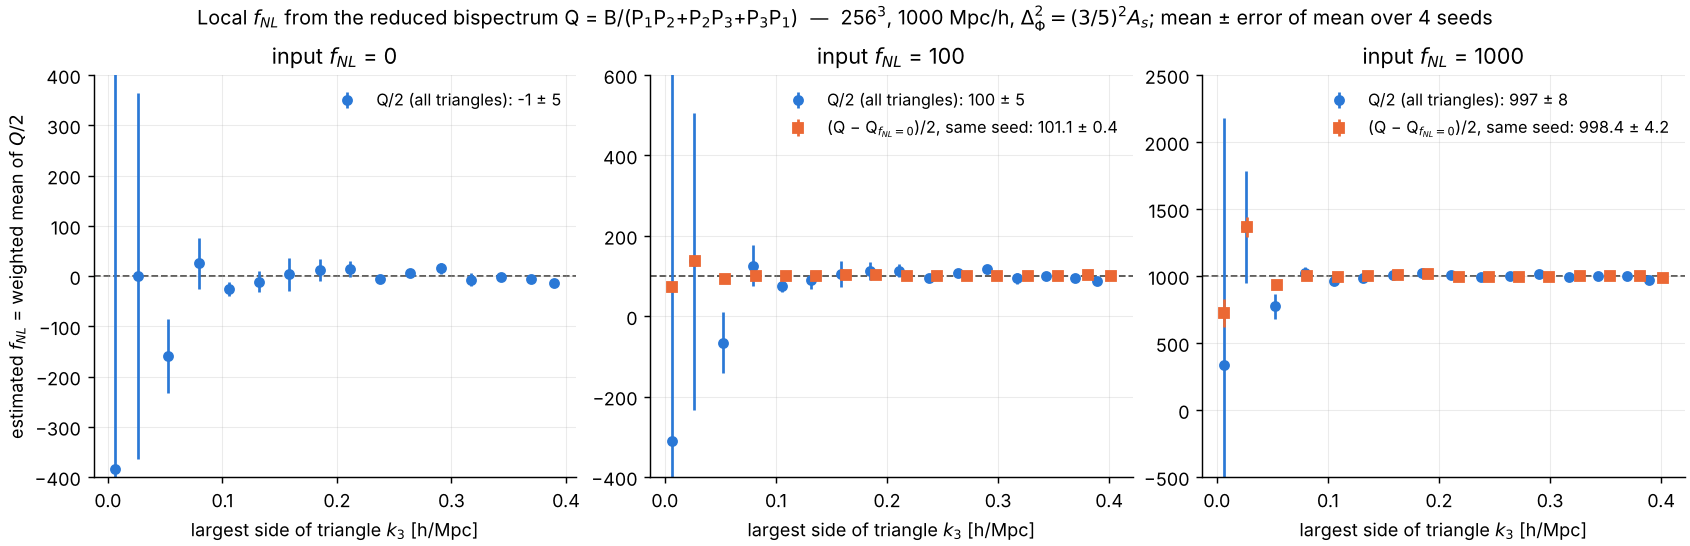
\includegraphics[width=\textwidth]{fnl_bispectrum}
\caption{Local $f_{\rm NL}$ recovered from the reduced bispectrum $Q=B/(P_1P_2+P_2P_3+P_3P_1)$ of non-Gaussian fields
($256^3$, $1000\Mpch$, mean and error over 4 seeds) for input $f_{\rm NL}=0$, 100 and 1000, as a function of the largest side of the
triangle. The same-seed difference $(Q-Q_{f_{\rm NL}=0})/2$ removes most of the cosmic variance of the Gaussian part. A standalone run
of \file{RandomFields} and \file{ComputePowerSpectra} with the method of \file{tests/test_fnl.cpp}.}
\label{fig:rf-fnl}
\end{figure}


\chapter{Lagrangian perturbation theory and initial conditions}\label{ch:lpt}
\chapterstatus{written}{2026-11-14}

Lagrangian perturbation theory (LPT) describes structure formation by the displacement of fluid elements from their
initial positions. It is the standard way to set up particle initial conditions, the analytic backbone of the COLA
method (\cref{ch:nbody-pm}), and a forward model for reconstruction and field-level inference. This chapter gives the
LPT equations and their solutions to third order, the arbitrary-order recursion, the de-aliasing of the nonlinear
terms, the augmented and spherical-collapse variants, redshift-space reconstruction, and glass particle loads.

\begin{modulebox}{LPT}
\file{LPT/DisplacementFields.h} (namespace \nsp{FML::COSMOLOGY::LPT}): 1LPT, 2LPT and 3LPT potentials and displacement
fields, the scale-dependent displacement, ALPT and spherical collapse, \code{compute_LPT_growth_factors_LCDM},
\code{_GeffGLCDM}; \file{LPT/Dealiasing.h}; \file{LPT/ArbitraryOrder.h}; \file{LPT/Reconstruction.h} (RSD removal);
\file{LPT/GrowthHistory.h}.\par
Documentation: \file{LPT/README.md}, \file{ARBITRARY_ORDER_DERIVATION.md}, \file{ARBITRARY_ORDER_API.md},
\file{ARBITRARY_ORDER_PLAN.md}, \file{SCIENCE_RESULTS.md}. Tests: \file{tests/test_lpt.cpp}, \file{LPT/tests}.
\end{modulebox}
\begin{modulebox}{GlassIC}
\file{GlassIC/GlassIC.h}, \file{GlassIC/LoadIO.h} (namespace \nsp{FML::GLASSIC}). Documentation:
\file{GlassIC/README.md}, \file{GlassIC/tests/RESULTS.md}.
\end{modulebox}

\section{The Lagrangian equations of motion}\label{sec:lpt-equations}

A fluid element that starts at the Lagrangian position $\vq$ is at the Eulerian position
\begin{equation}
\vx(\vq,a)=\vq+\bm\Psi(\vq,a).
\end{equation}
With the deformation tensor $F_{ij}=\delta_{ij}+A_{ij}$, $A_{ij}=\partial\Psi_i/\partial q_j$, and its determinant
$J=\det F$, mass conservation is simply $1+\delta(\vx)=1/J(\vq)$. The Eulerian divergence of the equation of motion
$\ddot\vx+2H\dot\vx=-\nabla_x\Phi/a^2$ (comoving coordinates, $\nabla^2_x\Phi=\frac32\Om_mH^2a^2\delta$ in GR) becomes,
after multiplying by $J$ and with the cofactor matrix $C_{ij}=\partial J/\partial F_{ij}$,
\begin{equation}
\sum_{ij}C_{ij}\left(\partial_t^2+2H\partial_t\right)A_{ij}=\frac32\Om_m(a)H^2\,(J-1).
\label{eq:lpt-longitudinal}
\end{equation}
The initial flow is irrotational, which in Lagrangian coordinates is the Cauchy invariant: $F^T\,\dd F/\dd t$ is
symmetric. Expanding $\bm\Psi=\sum_n\bm\Psi^{(n)}$ order by order in the linear density gives, at each order, a
Poisson-type equation for the longitudinal part $\nabla_q\cdot\bm\Psi^{(n)}$ and, from third order, an equation for
the transverse part $\nabla_q\times\bm\Psi^{(n)}$, sourced by products of lower orders \cite{Bouchet1995,Matsubara2015}.

\section{First, second and third order}\label{sec:lpt-123}

Each order factorises into a growth factor (\cref{ch:growth-transfer}) and a spatial field, which \fml{} stores as
potentials: $\bm\Psi^{(1)}=\nabla\phi^{(1)}$, $\bm\Psi^{(2)}=\nabla\phi^{(2)}$,
$\bm\Psi^{(3)}=\nabla(\phi^{(3a)}+\phi^{(3b)})+\nabla\times\bm A^{(3)}$. With $H_{ij}=\partial_i\partial_j\phi^{(1)}$,
\begin{equation}
Q(A,B)=\Tr A\,\Tr B-\Tr(AB),\qquad K_i(A,B)=\epsilon_{ijk}\sum_lA_{lj}B_{lk},
\end{equation}
and $\nabla^2\chi=\frac12Q(H,H)=\sum_{i>j}(H_{ii}H_{jj}-H_{ij}^2)$, the potentials returned by
\code{compute_3LPT_potential_fourier} are, at the time of the input density $\delta$ (in units of the box),
\begin{align}
\nabla^2\phi^{(1)}&=-\delta, & \phi^{(2)}&=-\tfrac37\chi,\label{eq:lpt-potentials}\\
\nabla^2\phi^{(3a)}&=-\tfrac13\det H, & \nabla^2\phi^{(3b)}&=\tfrac{5}{21}Q\!\left(H,\nabla\nabla\chi\right),\qquad
\nabla^2\bm A^{(3)}=\tfrac17\bm K\!\left(H,\nabla\nabla\chi\right),\nonumber
\end{align}
which include the Einstein--de Sitter amplitudes of the growing modes (the Zel'dovich approximation is the first
order alone; $-3/7$ is the familiar 2LPT factor \cite{Scoccimarro1998,Crocce2006}). In EdS the $n$-th order grows as
$D^n$, so at another time and its velocity
\begin{equation}
\bm\Psi=D\bm\Psi^{(1)}+D^2\bm\Psi^{(2)}+D^3\bm\Psi^{(3)},\qquad
\frac{\dd\bm\Psi}{\dd t}=\frac{\dd\ln D}{\dd t}\left(D\bm\Psi^{(1)}+2D^2\bm\Psi^{(2)}+3D^3\bm\Psi^{(3)}\right),
\label{eq:lpt-velocity}
\end{equation}
which is what \code{compute_3LPT_displacement_field} returns (with $D=1$ at the time of $\delta$ and the units of
\code{dlogDdt} setting those of the velocity). In other cosmologies and theories of gravity the user, or
SimulationCode, multiplies each order by its own growth factor $D_1$, $D_2$, $D_{3a}$, $D_{3b}$ relative to the EdS
amplitude and uses the rates $f_i$; \cls{GrowthHistory} provides $D_1$, $D_2$ and their rates for this (and for the
$N$-body time stepping), with the peculiar velocity $v=a^2E f_1D_1\Psi^{(1)}+\ldots$ in the code velocity
$v=a^3E\,\dd x/\dd a$.

\paragraph*{Scale-dependent growth.} When the linear growth depends on scale (massive neutrinos, $f(R)$)
\code{from_LPT_potential_to_displacement_vector_scaledependent} applies a ratio $D(k,a)/D(k,a_{\rm ini})$ to the
potential in Fourier space before taking the gradient. Higher-order kernels with scale-dependent growth are
approximated by the EdS shape with the scale-dependent amplitude.

\begin{implementation}[Implementation: low-order LPT on the grid]
\begin{itemize}
\item All derivatives are spectral: $\partial_i\to ik_i$, $\nabla^{-2}\to-1/k^2$, the DC mode set to zero.
\item \emph{Nyquist convention}: for an even mesh the Nyquist mode $n_i=N_{\rm mesh}/2$ is its own mirror image, so
      odd ($ik_i$) and mixed ($k_ik_j$, $i\ne j$) derivatives of it depend on a sign choice and break reflection
      symmetry. They are set to zero (the derivative of the band-limited field there), while $k_i^2$ is kept; the
      results are then covariant under $x_i\to-x_i$, as in \file{TidalTensor/Hessian.h}. The same kernel is the
      continuous gradient of the PM force.
\item \emph{Memory}: the 3LPT construction keeps the first-order Hessian and streams the second-order Hessian in two
      batches through $N$ work grids: about 17 full grids at peak in 3D with all potentials and the curl, before the
      caller's outputs and FFT workspace.
\item 2D is supported (the vector potential then has only a $z$ component, $\nabla\times(A\hat z)=(\partial_yA,-\partial_xA)$).
\end{itemize}
\end{implementation}

\begin{cppcode}[Displacement fields to third order]
#include <FML/LPT/DisplacementFields.h>
using namespace FML::COSMOLOGY::LPT;

// delta_fourier: the linear density at the initial time (Fourier space, box units)
std::array<FML::GRID::FFTWGrid<3>, 3> Psi, dPsidt;
double dlogDdt = H_ini * f_ini;                          // sets the units of dPsidt
compute_3LPT_displacement_field<3>(delta_fourier, Psi, dPsidt, dlogDdt,
                                   /*ignore_curl=*/false, Dealiasing::Padding);
// Or the potentials, to scale each order with its own growth factor:
FML::GRID::FFTWGrid<3> phi1, phi2, phi3a, phi3b;  std::array<FML::GRID::FFTWGrid<3>, 3> A;
compute_3LPT_potential_fourier<3>(delta_fourier, phi1, phi2, phi3a, phi3b, A, false, Dealiasing::Padding);
\end{cppcode}

\section{De-aliasing the nonlinear terms}\label{sec:lpt-dealiasing}

The second- and third-order sources are products of fields evaluated in real space. On a grid the product of two
band-limited fields has modes up to twice (three times for cubic terms) the original bandwidth, which fold back onto
the resolved modes. With \code{Dealiasing::Padding} the normalised Fourier coefficients are embedded in a larger work
grid, the sources and potentials are computed there, and the results are cropped to the original mesh
\cite{Michaux2021}: at least $3/2$ of the width in every dimension for 2LPT (the quadratic rule) and at least twice
for 3LPT. The intermediate 2LPT potential keeps its full bandwidth on the work mesh while the third-order products are
formed; cropping it early would lose physical mode couplings. Work widths are rounded up to an even number divisible by
the number of MPI tasks; the spectral remapping exchanges only retained coefficients with chunked messages and never
replicates the grid. Only wave vectors with $2|n_i|<N_{\rm mesh}$ in every dimension are copied, so even-mesh
Nyquist planes are zeroed (also in the returned 1LPT potential); there is no radial cutoff or smoothing of the
sub-Nyquist modes. The cost is substantial: in 3D the work grids are $3.375\times$ (2LPT) and $8\times$ (3LPT) larger.
The default is \code{Dealiasing::None}, which keeps the original calculation. SimulationCode, ALPT and the
non-Gaussian generator do not enable it automatically.

\section{Arbitrary order}\label{sec:lpt-arbitrary}

\file{LPT/ArbitraryOrder.h} computes the growing-mode EdS solution to a user-selected order, with longitudinal and
transverse parts. With $g=a/a_{\rm ref}$ and no factorials,
$\bm\Psi(\vq,a)=\sum_{n\ge1}g^n\bm\Psi_n(\vq)$, $\nabla\cdot\bm\Psi_1=-\delta_{\rm ref}$. In EdS
$(\partial_t^2+2H\partial_t)g^n=H^2\lambda_ng^n$ with $\lambda_n=n(n+\frac12)$, so at order $n\ge2$ the unknown appears
in \cref{eq:lpt-longitudinal} only as $(\lambda_n-\frac32)\nabla\cdot\bm\Psi_n$. Matsubara's recursion
\cite{Matsubara2015} (Sec.~IV, Eqs.~62--64, EdS limit) gives, with $A^{(r)}=\nabla\bm\Psi_r$ and
$R(A,B,C)=\epsilon_{ijk}\epsilon_{pqr}A_{ip}B_{jq}C_{kr}$,
\begin{align}
d_n\equiv\nabla\cdot\bm\Psi_n&=-\frac12\sum_{\substack{r+s=n\\ r\le s}}M_{rs}
\left[1-\frac{4rs}{(2n+3)(n-1)}\right]Q(A^{(r)},A^{(s)})\nonumber\\
&\quad-\frac16\sum_{\substack{r+s+t=n\\ r\le s\le t}}M_{rst}\left[1-\frac{4(rs+st+tr)}{(2n+3)(n-1)}\right]
R(A^{(r)},A^{(s)},A^{(t)}),\\
\bm c_n\equiv\nabla\times\bm\Psi_n&=\sum_{\substack{r+s=n\\ r<s}}\frac{s-r}{n}\,\bm K(A^{(r)},A^{(s)}),
\end{align}
with multiplicities $M_{rs}=1$ for equal and 2 for different orders, and $M_{rst}=1$, 3 or 6 for three, two or no equal
orders. The first coefficients are $d_2=-\frac3{14}Q_{11}$, $d_3=-\frac59Q_{12}-\frac1{18}R_{111}$,
$\bm c_3=\frac13\bm K_{12}$, $d_4=-\frac7{11}Q_{13}-\frac{17}{66}Q_{22}-\frac{13}{66}R_{112}$, $\bm c_4=\frac12\bm K_{13}$.
There is no transverse part at orders 1 and 2, and from order 4 the transverse displacements of lower orders feed the
scalar sources through their full gradients. The vector is recovered by the Helmholtz inversion
$\bm\Psi_n(\vk)=[-i\vk\,d_n(\vk)+i\vk\times\bm c_n(\vk)]/k^2$; the velocity follows from
$\dd\bm\Psi/\dd\ln a=\sum_nng^n\bm\Psi_n$.

\begin{implementation}[Implementation: arbitrary order]
Products are formed with conservative full-bandwidth work meshes (widths exceed $2PK$ for order $P$ and input support
$K$), so high orders on full-support fields are very expensive: \code{plan_eds_lpt} reports the owned memory first and
\code{max_owned_bytes_per_rank} limits it. Outputs can be retained per order or streamed, and intermediate fields
cached or recomputed. The cubic mixed determinant is summed as paired $2\times2$ minors so that exactly rank-one
(plane-wave) deformations have exactly zero nonlinear sources. Empty MPI slabs are not supported; general cosmologies
and automatic SimulationCode wiring are separate work.
\begin{cppcode}
EdSLPTOptions options;
options.max_order = 6;
options.input_mode_limit = {1, 1, 1};                 // the strictly sub-Nyquist support of the seed
options.max_owned_bytes_per_rank = 512ULL << 20;
auto plan   = plan_eds_lpt(delta_ref, options, EdSLPTOutput::RetainOrders);
auto fields = compute_eds_lpt(delta_ref, options);
auto sums   = fields.evaluate(0.5, options.max_owned_bytes_per_rank);   // Psi and dPsi/dln a at g = 0.5
\end{cppcode}
\end{implementation}

\begin{validation}[Validation: LPT]
\begin{itemize}
\item The 1/2/3LPT fields (with and without padding, including the transverse third order) against independent sparse
      integer-wave-vector convolutions without wrapping (\file{tests/test_lpt.cpp}, 84 checks).
\item Arbitrary order: every Fourier coefficient against an independent Python oracle that extracts the coefficients
      of the original determinant/cofactor equations and Cauchy invariants, through order 6 for a fixture of three
      non-coplanar waves with unequal complex amplitudes (relative errors $2\times10^{-15}$ in double, $4\times10^{-7}$ in
      float); Matsubara's explicit kernels through order 4; translations, reflections, permutations, plane-wave
      exactness, and identical results serially, with OpenMP and on 1, 2 and 4 MPI ranks.
\item The example \file{LPT/example} reports per-order norms and the minimum of $\det(I+\nabla\bm\Psi)$: a negative
      Jacobian marks shell crossing, beyond which single-stream LPT is not valid.
\end{itemize}
\end{validation}

\section{Augmented LPT and spherical collapse}\label{sec:lpt-alpt}

On small scales LPT overshoots: particles stream through collapsed regions. The spherical-collapse approximation of
Bernardeau \cite{Bernardeau1994} replaces the divergence of the displacement by that of a spherical top hat,
\begin{equation}
\nabla\cdot\bm\Psi_{\rm SC}=3\left(\sqrt{\max\left(1-\tfrac23\delta(\vq,a),0\right)}-1\right),\qquad
\delta(\vq,a)=\frac{D(a)}{D(a_{\rm ini})}\delta_{\rm ini}(\vq),
\end{equation}
which equals the 1LPT divergence to linear order (\code{compute_spherical_collapse_potential}). Augmented LPT (ALPT)
\cite{KitauraHess2013} combines 2LPT on large scales with spherical collapse on small scales,
\begin{equation}
\phi_{\rm ALPT}=\phi_{\rm SC}+\mathcal S_R*\left(\phi^{(1)}+\phi^{(2)}-\phi_{\rm SC}\right),
\end{equation}
with a smoothing filter $\mathcal S_R$ (Gaussian, top-hat or sharp-$k$) of scale $R$
(\code{compute_ALPT_potential_fourier}).

\section{Particle initial conditions}\label{sec:lpt-ic}

Particle initial conditions combine the pieces of \cref{ch:growth-transfer,ch:random-fields} and this chapter:
\begin{enumerate}
\item a Gaussian (or non-Gaussian) realisation of the linear CDM+baryon density at the initial redshift, from the
      transfer provider and the growth factors (back-scaled or not);
\item the LPT potentials to order \param{ic_LPT_order} (1, 2 or 3), with each order scaled by its growth factor;
\item particles on a regular lattice (or a glass, \cref{sec:lpt-glass}) displaced by $\bm\Psi(\vq)$, interpolated from
      the grid, with velocities from \cref{eq:lpt-velocity} and the growth rates of each order.
\end{enumerate}
Two species, massive-neutrino particles and the $N$-body gauge are described in \cref{ch:growth-transfer,ch:simulation-code}.
For COLA the LPT fields are kept for the whole run. SimulationCode can also start from an existing snapshot
(\code{ic_random_field_type = read_particles} or \code{read_phases}), reconstructing the density by mass assignment
and the LPT fields from it, or exactly from the particles' displacements and velocities
(\param{ic_reconstruct_exact}).

\section{Redshift-space reconstruction}\label{sec:lpt-reconstruction}

\code{RSDReconstructionFourierMethod} removes redshift-space distortions from tracers in a periodic box with a fixed line
of sight $\hat{\bm r}$. In linear theory the displacement $\bm\Psi$ of the tracers (bias $b$, $\beta=f/b$) satisfies
\begin{equation}
\nabla\cdot(b\bm\Psi)+\beta\nabla\cdot\left[(b\bm\Psi\cdot\hat{\bm r})\hat{\bm r}\right]=-\delta_{\rm tracer},
\end{equation}
which is solved in Fourier space assuming that the second term is curl free, after smoothing the density with a filter
of scale $R$; the RSD shift $\bm\Psi_{\rm rsd}=\beta(b\bm\Psi\cdot\hat{\bm r})\hat{\bm r}$ is then subtracted. The
iterative scheme of Burden et al.\ \cite{Burden2015} starts from the observed positions $\bm s$, computes $b\bm\Psi_n$
from the density of the current estimate $\vx_{n-1}$ and sets $\vx_n=\bm s-\beta(b\bm\Psi_n(\bm s)\cdot\hat{\bm r})\hat{\bm r}$;
it converges for $\beta<1$ in 3--5 iterations. The assignment and interpolation windows are not deconvolved. Only a
periodic box with a fixed line of sight is supported here; BAO reconstruction of surveys is in \cref{ch:surveys}.
\code{particles_to_redshiftspace} applies $\bm s=\vx+c_v(\bm v\cdot\hat{\bm r})\hat{\bm r}$, with
$c_v=1/(100\,aH/H_0\,B)$ for peculiar velocities in km/s and the box $B$ in $\Mpch$ (a negative $c_v$ undoes it).

\section{Glass loads}\label{sec:lpt-glass}

A regular lattice imprints its symmetry on the early evolution; a \emph{glass}, a particle distribution with no
preferred directions and very little power on large scales, is the usual alternative. \file{GlassIC/GlassIC.h}
generates periodic equal-mass glasses by evolving a Poisson load (\code{poisson_load}, positions from Philox streams
keyed by the seed and the particle ID, so independent of the task and thread counts) under \emph{repulsive} gravity
with damping, until it settles:
\begin{itemize}
\item the force is softened periodic P$^3$M gravity with the sign reversed for both the long-range (CIC, Gaussian
      split, continuous gradient, compensation of the assignment and interpolation windows) and the short-range part
      (the spline kernel of \cref{ch:short-range}); reversing only the mesh force would leave close pairs unconstrained;
\item each step holds the acceleration fixed for an exact damped kick,
      $\bm v_{\rm next}=e^{-\gamma\Delta t}\bm v+\frac{1-e^{-\gamma\Delta t}}{\gamma}\bm a$, $\vx_{\rm next}=\vx+\Delta t\,\bm v_{\rm next}$,
      with a global velocity factor limiting the largest step to \code{max_step_spacing} times the mean spacing;
\item convergence requires the rms force and velocity below their tolerances for \code{stable_steps} consecutive steps;
      the result reports \code{Converged}, \code{MaximumSteps} or \code{NonFinite} and the history.
\end{itemize}
A converged residual alone does not make a load suitable for science: its discreteness power, anisotropy and
close-pair statistics should be checked at the intended particle number. Loads are saved in a versioned, sharded
text format (\file{LoadIO.h}) that can be read back with a different number of tasks. Perturbations are applied with
\code{apply_3lpt(load, delta_fourier, dlogDdt, dealiasing)} (EdS-factorised 3LPT sampled by CIC at the glass
positions) or \code{apply_fields} (precombined displacement and velocity fields, e.g.\ with other growth
prescriptions), and \code{density_from_provider} bridges a transfer provider to the Philox generator. Multi-species
glasses and SimulationCode integration are future work.

\begin{cppcode}[A glass load with 3LPT initial conditions]
#include <FML/GlassIC/GlassIC.h>
using namespace FML::GLASSIC;
auto load = poisson_load(32768, 12345, 250.0);   // count, seed, box [Mpc/h]
Options options;                                  // mesh = 0: smallest task multiple >= 3 N^(1/3)
options.max_steps = 3000;
auto result = relax(load, options);              // check result.status
density_from_provider(delta, provider, Species::CDMBaryon, a_ini, 250.0, field_seed, /*fixed=*/false);
apply_3lpt(load, delta, dlogDdt, FML::COSMOLOGY::LPT::Dealiasing::Padding);
\end{cppcode}


\part{Simulations}
\chapter{Particle--mesh gravity, time stepping and COLA}\label{ch:nbody-pm}
\chapterstatus{written}{2026-11-26}

This chapter describes how \fml{} moves particles under their own gravity: the comoving equations of motion and their
units, the particle--mesh (PM) force with its choices of Green's function, gradient, assignment and anti-aliasing,
the four time integrators (Quinn, Tassev, FastPM and BullFrog), including velocity friction and several species, and
the COLA method, in its scale-independent and scale-dependent forms. Short-range corrections to the PM force are in
\cref{ch:short-range}; the complete simulation program in \cref{ch:simulation-code}.

\begin{modulebox}{NBody}
\file{NBody/NBody.h} (namespace \nsp{FML::NBODY}): density assignment, Poisson solve, forces, kick and drift;
\file{NBody/ForceOptions.h} (\cls{ForceOptions}); \file{NBody/TimeStepping.h}, \file{NBody/TimeStepTypes.h}
(\cls{TimeStepping}, \cls{TimestepOptions}); \file{LPT/GrowthHistory.h}.\par
SimulationCode: \file{src/KickDrift.h}, \file{src/COLA.h}, \file{src/SimulationStep.h}, \file{src/SpeciesTimeStepping.h},
\file{src/TimeStepping.h}.\par
Documentation: \file{NBody/ForceOptions.md}, \file{NBody/TimeStepping.md}, \file{SimulationCode/EVOLUTION.md},
\file{SimulationCode/DYNAMICS.md}.
\end{modulebox}

\section{Equations of motion}\label{sec:nbody-eom}

Particles move in comoving coordinates $\vx$, in units of the box size $B$. With the canonical code velocity
\begin{equation}
\bm v\equiv a^3E(a)\frac{\dd\vx}{\dd a}=\frac{a^2}{H_0}\frac{\dd\vx}{\dd t},
\end{equation}
the equations of motion of a cold particle are
\begin{equation}
\frac{\dd\vx}{\dd a}=\frac{\bm v}{a^3E(a)},\qquad \frac{\dd\bm v}{\dd a}=-\frac{\nabla\phi}{a^3E(a)},\qquad
\nabla^2\phi=\frac32\Om_m\,a\,\mu(k,a)\,\delta,
\label{eq:nbody-eom}
\end{equation}
where $\phi$ is the peculiar potential in units of $(H_0B)^2$ and $\nabla$ is with respect to $\vx$ in box units. The
\emph{force prefactor} $C(a)=\frac32\Om_ma\,\mu$ carries the time dependence of the force; in GR $\mu=1$. A velocity
friction $\Gamma(a)$, $\dd\bm v/\dd\ln a=-\Gamma\bm v+\ldots$ (dark scattering, coupled quintessence), is optional.

\section{The particle--mesh force}\label{sec:nbody-pm}

A PM step computes $\delta$ on a grid of $N_{\rm mesh}^3$ cells (\param{force_nmesh}), solves the Poisson equation in
Fourier space and interpolates the force back to the particles:
\begin{equation}
\bm F(\vk)=-i\bm D(\vk)\,G(\vk)\,C(a)\,\frac{\delta(\vk)}{W^{2}(\vk)}\quad(\text{deconvolved}),\qquad
\bm F_p=\sum_{\rm cells}W(\vx_p-\vx_{\rm cell})\bm F(\vx_{\rm cell}),
\end{equation}
with the assignment window $W$ of order $p$ (NGP, CIC, TSC, PCS, PQS; \cref{ch:mass-assignment}),
$W(\vk)=\prod_j[\mathrm{sinc}(k_j\Delta x/2)]^p$, used both to assign and to interpolate so that the self-force vanishes
and momentum is conserved \cite{HockneyEastwood1988}. In SimulationCode the kernel is \param{force_density_assignment_method}
(CIC by default) and \param{force_interpolation_method} chooses how the force reaches the particles: with the same kernel
(\code{assignment}), or by evaluating its Fourier series exactly at the particles (\code{nufft}; \code{fiducial}, the
default, does this when the density is also a NUFFT, so that there is still no self-force). The Green's function $G$ and the gradient $\bm D$ (\cls{ForceOptions}) are described in \cref{sec:nbody-kernels}. There are no global defaults: each call takes its \cls{ForceOptions}.

\begin{cppcode}[A PM force]
#include <FML/NBody/NBody.h>
FML::NBODY::ForceOptions options;
options.laplace_kernel  = FML::NBODY::DISCRETE_GREENS_FUNCTION_FROM_TWO_POINT;
options.gradient_kernel = FML::NBODY::DISCRETE_FOUR_POINT_GRADIENT;
options.deconvolve      = false;
double norm = 1.5 * OmegaM * a;                       // the Poisson prefactor C(a)
FML::NBODY::compute_force_from_density_fourier<3>(density_fourier, force, "CIC", norm, options);
\end{cppcode}

\subsection{The force kernels}\label{sec:nbody-kernels}

A PM force is built from three kernels: the Green's function $G(\vk)$ that inverts the Laplacian, the gradient
$\bm D(\vk)$ that differentiates the potential ($\nabla\to i\bm D$) and the assignment window $W(\vk)$. With
$\Delta x=1/N_{\rm mesh}$ (box units), $\delta(\vk)$ the Fourier transform of the assigned density and $C$ the Poisson
prefactor ($\nabla^2\Phi=C\delta$), the force on the grid is
\begin{equation}\label{eq:nbody-force-kernels}
\Phi(\vk)=G(\vk)\,C\,\delta(\vk),\qquad
\bm F(\vk)=-i\bm D(\vk)\,\frac{\Phi(\vk)}{W^{n}(\vk)},\qquad
W(\vk)=\prod_{j}\left[\mathrm{sinc}\frac{k_j\Delta x}{2}\right]^{p},
\end{equation}
with $n=0$ (\code{deconvolve = false}, the default) or $n=$ \code{deconvolve_window_power} (2: assignment and
interpolation with the window; 1 if one of them is exact, as with the NUFFT), and $p$ the assignment order
(1 NGP, 2 CIC, 3 TSC, 4 PCS, 5 PQS). The exact force of the band-limited density is $G=-1/k^2$ and $\bm D=\vk$. The
discrete kernels are the Fourier transforms of finite-difference stencils: a stencil acting on $\phi(x_i+l\Delta x)$
becomes a multiplication by $e^{ilk\Delta x}$, so a symmetric difference gives $i\sin$ and a symmetric second difference
$\cos$. All kernels act direction by direction, $\bm D=(D(k_1),D(k_2),D(k_3))$ and
$G=-1/\sum_jL(k_j)$, where $L(k)$ is minus the one-dimensional Laplacian. With $x=k\Delta x$ ($x=\pi$ at the
grid Nyquist frequency $k_{\rm Ny}=\pi/\Delta x$):

\paragraph{Green's functions} (\cls{GreensFunctionLaplaceOperatorKernels}, \param{force_greens_function_kernel};
\code{greens_function_laplace_operator_fourier} in \file{NBody/NBody.h})
\begin{center}\small
\begin{tabularx}{\textwidth}{@{}llXl@{}}
\toprule
Name & Real-space stencil for $\partial^2\phi$ & $L(k)\,\Delta x^2$ & Small $x$ \\
\midrule
\code{continuous} & (spectral) & $x^2$ & exact \\
\code{discrete_2pt} & $\dfrac{\phi_{i+1}-2\phi_i+\phi_{i-1}}{\Delta x^2}$ & $4\sin^2\dfrac{x}{2}=2(1-\cos x)$ & $x^2\left(1-\dfrac{x^2}{12}\right)$ \\[1.5ex]
\code{discrete_4pt} & $\dfrac{-\phi_{i+2}+16\phi_{i+1}-30\phi_i+16\phi_{i-1}-\phi_{i-2}}{12\Delta x^2}$ & $\dfrac{15-16\cos x+\cos 2x}{6}$ & $x^2\left(1-\dfrac{x^4}{90}\right)$ \\
\bottomrule
\end{tabularx}
\end{center}
\code{discrete_2pt} is the 7-point Laplacian in 3D, the discrete Green's function of \citet{HockneyEastwood1988}; it is
second order and makes the potential too large at high $k$ ($L/k^2=0.81$ at $k_{\rm Ny}/2$ and $4/\pi^2=0.41$ at
$k_{\rm Ny}$ along an axis). \code{discrete_4pt} is the fourth-order (5-point per direction) stencil ($L/k^2=0.95$ at
$k_{\rm Ny}/2$, $0.54$ at $k_{\rm Ny}$). Both vanish only at $\vk=0$, where $G$ is set to zero (the mean density does
not source the potential). Until November 2026 \code{discrete_4pt} was $L=D_4^2$, the square of the four-point gradient
below; that vanishes at $k_{\rm Ny}$, so the modes near it got a potential up to $\sim10^4$ times too large and runs
with it blew up. Since the potential is computed once and then differentiated, $G$ and $\bm D$ need not come from the
same stencil: composing the two-point gradient twice gives the wide stencil
$(\phi_{i+2}-2\phi_i+\phi_{i-2})/(4\Delta x^2)$, with $L=\sin^2x/\Delta x^2$, not \code{discrete_2pt}.

\paragraph{Gradients} (\cls{GradientKernels}, \param{force_gradient_kernel}; \code{gradient_kernel_fourier})
\begin{center}\small
\begin{tabularx}{\textwidth}{@{}llXl@{}}
\toprule
Name & Real-space stencil for $\partial\phi$ & $D(k)\,\Delta x$ & Small $x$ \\
\midrule
\code{continuous} & (spectral) & $x$ ($0$ at $x=\pi$) & exact \\
\code{discrete_2pt} & $\dfrac{\phi_{i+1}-\phi_{i-1}}{2\Delta x}$ & $\sin x$ & $x\left(1-\dfrac{x^2}{6}\right)$ \\[1.5ex]
\code{discrete_4pt} & $\dfrac{-\phi_{i+2}+8\phi_{i+1}-8\phi_{i-1}+\phi_{i-2}}{12\Delta x}$ & $\dfrac{8\sin x-\sin 2x}{6}$ & $x\left(1-\dfrac{x^4}{30}\right)$ \\[1.5ex]
6th order (FD only) & $\dfrac{45\delta_1\phi-9\delta_2\phi+\delta_3\phi}{60\Delta x}$, $\delta_l\phi=\phi_{i+l}-\phi_{i-l}$ & $\dfrac{45\sin x-9\sin 2x+\sin 3x}{30}$ & $x\left(1-\dfrac{x^6}{140}\right)$ \\
\bottomrule
\end{tabularx}
\end{center}
$D/k$ is $0.64$, $0.85$ and $0.93$ at $k_{\rm Ny}/2$ for the 2-, 4- and 6-point stencils. Every gradient is zero for the
Nyquist component $k_j=k_{\rm Ny}$ of an even mesh: the discrete ones because $\sin(\pi)=0$, the continuous one by
construction, since that mode is its own mirror image and $ik_j$ would depend on the sign chosen for it (FFTW's
$+k_{\rm Ny}$); with zero there the force of a reflected density is the reflected force. The finite-difference force
(\code{compute_force_from_potential_real}, \param{force_use_finite_difference_force} with
\param{force_finite_difference_stencil_order} $=2,4,6$) applies the stencils in real space to the potential computed
with the chosen Green's function; orders 2 and 4 give the same force as the Fourier gradients \code{discrete_2pt} and
\code{discrete_4pt} (to $10^{-15}$), order 6 exists only there.

\paragraph{The force of a combination.} Without the window, the force of a single mode relative to the exact force
$\vk/k^2$, along the wave vector, is
\begin{equation}
\frac{F_{\rm PM}}{F_{\rm exact}}=\frac{|\vk|\,\hat{\vk}\cdot\bm D(\vk)}{\sum_jL(k_j)}
\;\xrightarrow{\ \vk\parallel\hat{\bm e}_1\ }\;\frac{k\,D(k)}{L(k)} .
\end{equation}
Along an axis, at small $x$, this is $1$ (continuous/continuous), $1-x^2/6$ (two-point $\bm D$, continuous $G$),
$1-x^4/30$ (four-point $\bm D$, continuous or four-point $G$), $1-x^2/12$ (two-point $\bm D$ and $G$) and $1+x^2/12$
(four-point $\bm D$, two-point $G$). The discrete kernels are anisotropic: the same $|\vk|$ along the diagonal
$(1,1,1)/\sqrt3$ has each component $\sqrt3$ times smaller and is closer to exact. \Cref{fig:nbody-force-kernels} shows
the kernels; some values:
\begin{center}\small
\begin{tabular}{@{}llcccc@{}}
\toprule
& & \multicolumn{2}{c}{along an axis} & \multicolumn{2}{c}{along the diagonal} \\
$\bm D$ & $G$ & $k_{\rm Ny}/4$ & $k_{\rm Ny}/2$ & $k_{\rm Ny}/4$ & $k_{\rm Ny}/2$ \\
\midrule
continuous & continuous & 1 & 1 & 1 & 1 \\
\code{discrete_2pt} & continuous & 0.900 & 0.637 & 0.966 & 0.869 \\
\code{discrete_4pt} & continuous & 0.988 & 0.849 & 0.999 & 0.980 \\
\code{discrete_2pt} & \code{discrete_2pt} & 0.948 & 0.785 & 0.983 & 0.931 \\
\code{discrete_4pt} & \code{discrete_2pt} & 1.041 & 1.047 & 1.016 & 1.050 \\
\code{discrete_4pt} & \code{discrete_4pt} & 0.992 & 0.898 & 0.999 & 0.986 \\
continuous & \code{discrete_2pt} & 1.053 & 1.234 & 1.017 & 1.072 \\
\bottomrule
\end{tabular}
\end{center}
Pairing a discrete Green's function with the continuous gradient boosts the force at high $k$ (the potential is too
large and nothing compensates). These are the kernels alone: the window then multiplies the force by $W^{2-n}$ (CIC:
$W^2=0.66$ along an axis at $k_{\rm Ny}/2$), and the aliased images of the assignment add to it, which interlacing
(\param{force_interlacing_order}) reduces: the force is averaged over $M$ copies of the particles shifted by fractions of
a cell, and for the half-cell diagonal ($M=2$) the images at $\vk+2k_{\rm Ny}\bm n$ with odd $\sum_jn_j$ get the
phase $-1$ and cancel. On a grid finer than the particle grid the kernels also decide how the lattice signal at the
grid Nyquist frequency reaches the particles (next subsection), which is why SimulationCode's fiducial gradient is not
the continuous one there.

\begin{figure}[htbp]
\centering
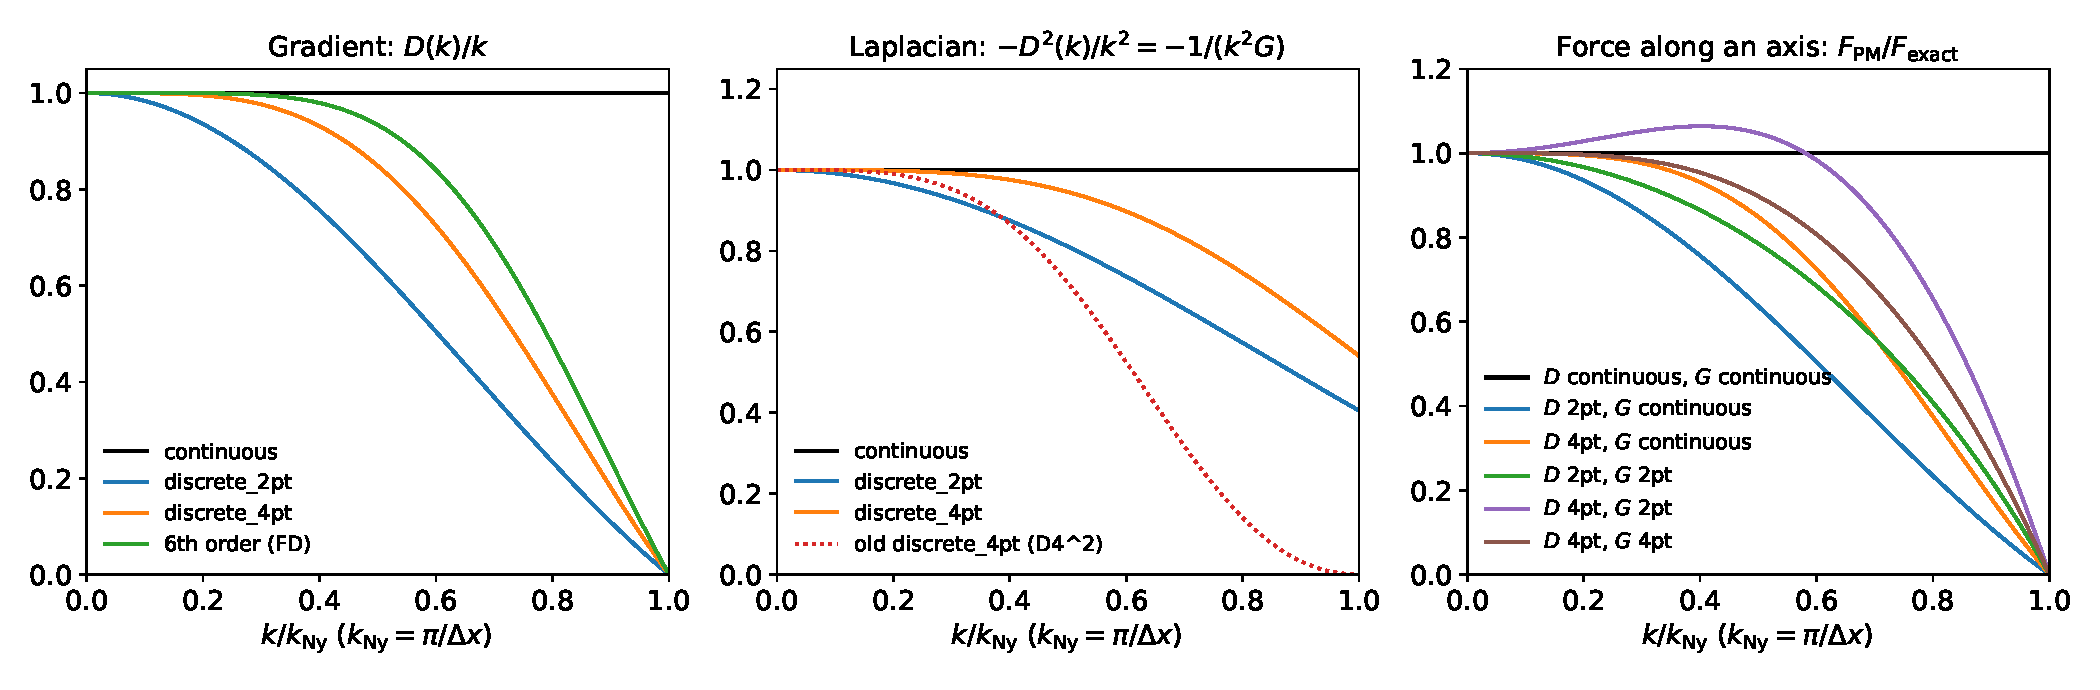
\includegraphics[width=\textwidth]{force_kernels}
\caption{The force kernels of \cls{ForceOptions} along a grid axis: the gradients $D(k)/k$ (\emph{left}; the sixth order
is the finite-difference force), the Laplacians $L(k)/k^2=-1/(k^2G)$ (\emph{middle}; dotted: the pre-November 2026
\code{discrete_4pt}, $D_4^2$, which vanishes at $k_{\rm Ny}$) and the force of the combinations relative to the exact
force, without the assignment window (\emph{right}). Made with \file{Documentation/tools/force_kernels_figure.py}.}
\label{fig:nbody-force-kernels}
\end{figure}

\paragraph{Choosing.} The library default (an omitted \cls{ForceOptions}) is continuous $G$ and $\bm D$ without
deconvolution. SimulationCode's \code{fiducial} is the continuous Green's function and, for the gradient, continuous
for $N_{\rm mesh}=N_p^{1/3}$, \code{discrete_4pt} for $N_p^{1/3}<N_{\rm mesh}\le3N_p^{1/3}$ and \code{discrete_2pt} for
finer grids, with the lattice offset by half a force cell. In the PM settings study ($64^3$ particles in
$250\Mpch$) \code{discrete_4pt} for $G$ gives $P(k)$ within $0.1\%$ of the continuous $G$ to
$k=0.3\hMpc$ and \code{discrete_2pt} $+8.5\%$; the larger effects come from the grid size and the window
(\cref{sec:nbody-pm}, \file{SimulationCode/tests/check_pm_settings.py}).

\begin{validation}[Validation: force kernels (\file{tests/test_nbody.cpp})]
\code{test_nbody} checks the \code{discrete_4pt} Green's function against its 5-point stencil (to $10^{-15}$) and that it is bounded at the Nyquist frequency ($k^2|G|\le1.85$), the plane-wave force $\sin(kx)\,D_4/L_4$ of the four-point kernels, that the force of a reflected density is the reflected force also for the Nyquist modes (which needs the zero Nyquist gradient), and that the finite-difference force equals the Fourier force of the same stencil, with and without deconvolution.
\code{check_pm_settings.py} (1--3 minutes) runs a $64^3$ simulation with each setting, \code{discrete_4pt} $G$
included, against a converged run.
\end{validation}

\subsection{The force grid, the lattice and the gradient kernel}

COLA and PM runs usually use a force grid 2--4 times finer than the particle grid. With an integer ratio
$m=N_{\rm mesh}/N_p^{1/3}$ the particles of a lattice start exactly on grid nodes, where the CIC kernel has a kink, so
the assigned density responds to the \emph{size} of the displacement: a rectified signal at the lattice frequency
(the grid Nyquist frequency for $m=2$). With the continuous gradient, which is large near Nyquist, this gives spurious
forces (the growth of single large-scale modes off by tens of per cent). SimulationCode's fiducial settings therefore
offset the lattice by half a force cell (\param{ic_lattice_offset}) and use the four-point gradient for grids up to
$3\times$ the particle grid and the two-point gradient for finer grids (\param{force_gradient_kernel}
\code{= fiducial}). With these, $P(k)$ at $z=0$ agrees with a $6\times$ TSC reference to $\lesssim1\%$ for $k\le0.4\hMpc$
on 2--4$\times$ grids, against $+10$--$14\%$ for the continuous kernel on a $2\times$ grid with particles on the nodes.

The plain library functions have no such defaults: \code{NBodyInitialConditions} puts the particles on the nodes and
an omitted \cls{ForceOptions} means the continuous gradient. In a linear test ($64^3$ particles, $N_{\rm mesh}=128$,
CIC, displacements much smaller than a cell) the growth of the first six modes is off by factors $0.5$--$3.8$; the
two-point gradient alone brings it to within $1\%$, the four-point gradient to within $9\%$ and TSC to within $4\%$,
while shifting the lattice with the continuous gradient still leaves $+5$--$24\%$. With realistic amplitudes the
particles leave the nodes early and the effect is smaller (in the \file{NBody/example} run the continuous gradient
gives $3$--$6\%$ more power at $k<0.03\hMpc$ than a TSC run, the two-point gradient agrees with it to $1$--$2\%$),
but with a finer force grid set
\code{options.gradient_kernel = FML::NBODY::DISCRETE_TWO_POINT_GRADIENT}, as \file{NBody/example} does
(details in \file{NBody/ForceOptions.md}).

\subsection{Accurate forces on a grid equal to the particle grid}

With $N_{\rm mesh}^3$ equal to the number of particles, CIC smooths the force twice and aliases it, so $P(k)$ is low on
all but the largest scales ($-13\%$ at $k=0.2\hMpc$ for $64^3$ particles in $256\Mpch$). Options for this case:
\begin{itemize}
\item \param{force_interlacing_order} $M>1$: the force is computed for $M$ copies of the particles shifted by fractions of
      a cell (2: the half-cell diagonal; 4: face diagonals; 8: all half-cell corners; 64: quarter cells), interpolated
      to the shifted particles and averaged, which cancels the leading aliasing of assignment and interpolation;
\item \param{force_deconvolve_window}: divide by $W^2(\vk)$; unstable alone, but with interlacing TSC or PCS with $M=2$
      plus deconvolution (as in the BullFrog work of List, Hahn and Rampf) gives $P(k)$ within $0.5\%$ of a converged
      reference for $k\le0.4\hMpc$ at $\sim7\times$ the cost of the CIC force;
\item \param{force_density_method} \code{= nufft}: the exact Fourier modes of the particles by a non-uniform FFT
      (\cref{ch:mass-assignment}, accuracy \param{force_nufft_epsilon}, default $10^{-5}$) and the force evaluated
      exactly at the particles; slightly better again at twice the cost;
\item \code{sheet}/\code{sheet_nufft}: spectral sheet interpolation, with \param{force_sheet_refinement}$^3$ tracers per
      particle placed by Fourier interpolation of the displacement field (mostly a library feature);
\item \param{force_early_method} \code{= interlaced} or \code{nufft} until \param{force_early_until_redshift}: an
      accurate force only at early times, when the particles are close to the lattice and CIC is worst (the interlaced
      force uses \param{force_early_interlacing_order} shifted grids with \param{force_early_density_assignment_method},
      default TSC, and deconvolution).
\end{itemize}
These options are only meant for $N_{\rm mesh}=N_p^{1/3}$: on finer grids the modes between the particle and grid
Nyquist frequencies are dominated by discreteness, and removing the smoothing there gives far too much power.

\subsection{The lattice-calibrated Green's function}

While the particles are close to a cubic lattice, the PM force on a linear mode differs from the true force by a factor
that follows from the lattice images alone. For a displacement $\bm\Psi(\vq)$ of particles on the lattice $\vq$ with
$N_{\rm mesh}=m\,N_p^{1/3}$, the assigned density of a mode $\vk$ below the particle Nyquist frequency contains the mode
itself and its images at $\vk+2k_{\rm Ny}^{(p)}\bm n$; interpolating the force back to the particles adds the images of
the grid. Summing the separable one-dimensional image sums (closed forms for CIC and the higher B-splines, with the
lattice offset and the interlacing shifts) gives the linear response $T(\vk)$ of the scheme, and a lattice-field term
$E(\vk)$ (for $m\ge3$) from the grid modes the lattice itself excites. \cls{LatticeGreensFunction}
(\file{NBody/LatticeGreensFunction.h}, \code{ForceOptions::lattice_greens}) multiplies the Green's function by
\begin{equation}
C(\vk)=\frac{1-E(\vk)}{T(\vk)-E(\vk)},
\end{equation}
which makes the linear force exact for particles near the lattice (for $m\ge2$ tapered from $0.7\,k_{\rm Ny}$ and capped
at 3). On a grid equal to the particle grid the exact correction is the ideal low-pass filter at the particle Nyquist
frequency, which is what the NUFFT force computes; on finer grids the modes between the two Nyquist frequencies are
discreteness and the NUFFT is not the right reference. With particles on the nodes of a finer grid CIC responds to the
size of the displacement and is not linear, so CIC needs the lattice offset (half a cell, or a quarter with two
interlaced grids). In linear runs of 20 steps the growth at $k_{\rm Ny}/2$ is then off by $+0.02\%$ (PCS, $1\times$),
$+0.07\%$ (CIC, $1\times$, offset by half a cell) and $+0.4\%$ (CIC, $2\times$). Once the particles have moved away
from the lattice the factor is no longer right (used throughout it is worse than PCS with interlacing and
deconvolution), so in SimulationCode it is an early force (\param{force_lattice_greens_function} until
\param{force_lattice_greens_until_redshift}, $\approx10$): a 1LPT start at $z=1000$ then gives $P(k,z=0)$ within
$0.1\%$ of 2LPT at $z=19$, at the cost of the CIC force.

\section{Time stepping}\label{sec:nbody-timestepping}

The steps are fixed before the run: the scale factors of the steps are uniform in $a$ (\code{linear}, default),
$\ln a$, $a^n$ (\code{powerlaw}) or the linear growth factor $D(a)$ (\code{growthfactor})
(\param{timestep_scalefactor_spacing}). Each step of \cls{TimeStepping} is
\begin{equation}
\bm v\leftarrow s\,\bm v+\Delta_K\,\bm F(\vx,a_{\rm pos}),\qquad \vx\leftarrow\vx+\Delta_D\,\bm v,
\end{equation}
with a velocity factor $s$ (1 without friction), a kick factor $\Delta_K$ and a drift factor $\Delta_D$, from
$(a_{\rm pos},a_{\rm vel})$ to $(a_{\rm pos}^{\rm new},a_{\rm vel}^{\rm new})$; $F$ is the force with the prefactor $C(a)$ of the
caller. Quinn, Tassev and FastPM are kick--drift--kick sequences (a staggering kick first, a synchronising kick last);
BullFrog is drift--kick--drift. A sequence has \code{nsteps + 1} entries.

\paragraph*{Quinn} \cite{Quinn1997}: the standard leapfrog with
\begin{equation}
\Delta_D=\int_{a_{\rm pos}}^{a_{\rm pos}^{\rm new}}\frac{\dd a}{a^3E},\qquad
\Delta_K=\int_{a_{\rm vel}}^{a_{\rm vel}^{\rm new}}\frac{\dd a}{a^3E}\frac{C(a)}{C(a_{\rm pos})}.
\end{equation}

\paragraph*{Tassev} \cite{Tassev2013}: the modified operators for COLA, which assume the residual velocity varies as
$a^{n_{\rm LPT}}$ (\param{timestep_cola_nLPT}, default $-2.5$):
\begin{equation}
\Delta_D=\int\frac{\dd a}{a^3E}\left(\frac{a}{a_{\rm vel}}\right)^{n_{\rm LPT}},\qquad
\Delta_K=\frac{(a_{\rm vel}^{\rm new})^{n_{\rm LPT}}-a_{\rm vel}^{n_{\rm LPT}}}{n_{\rm LPT}\,a_{\rm pos}^{n_{\rm LPT}-1}}\,
\frac{1}{a_{\rm pos}^3E(a_{\rm pos})}.
\end{equation}

\paragraph*{FastPM} \cite{Feng2016}: the factors are chosen so that the linear growing mode, $\vx=\vq+D\bm\Psi$,
$\bm v=G_p\bm\Psi$, $\bm F=G_f\bm\Psi$, is followed exactly for any step size:
\begin{gather}
\Delta_D=\frac{D(a_{\rm pos}^{\rm new})-D(a_{\rm pos})}{G_p(a_{\rm vel}^{\rm new})},\qquad
\Delta_K=\frac{G_p(a_{\rm vel}^{\rm new})-s\,G_p(a_{\rm vel})}{G_f(a_{\rm pos})},\\
G_p=a^3E\frac{\dd D}{\dd a},\qquad G_f=\tfrac32\Om_m\mu\,aD .
\end{gather}
With a scale-dependent growth $D(k,a)$ (a $G_{\rm eff}(k,a)$, massive neutrinos) FastPM is exact for one growth
history only: the drift factor is one number per step, while each mode needs its own $\Delta D(k)$. The kick can
depend on $k$, as the force is computed in Fourier space. With the velocity between two kicks the effective
$V_{n+1/2}(k)=[D(k,a_{n+1})-D(k,a_n)]/\Delta_D$, the common drift gives each mode its own growth, and the kick needs the
factor
\begin{equation}
R(k)=\frac{V_{\rm after}(k)-s\,V_{\rm before}(k)}{\Delta_K\,G_f(k,a_{\rm pos})},\qquad
G_f(k,a)=\tfrac32\,a\,\Om_m(a)E^2a^3\,\frac{G_{\rm eff}}{G}(a,k)\,S(a,k)\,D(k,a),
\end{equation}
on the force, with $V=G_p(k,a)$ at the start and after a synchronising step, and $G_f$ the right hand side of the
growth equation of the model ($S$: the source factor of massive neutrinos and interacting dark energy). Then every
linear mode is followed exactly for any step size. In SimulationCode this is the experimental option
\param{timestep_scaledependent_kick}, implemented in \file{SimulationCode/src/ScaleDependentKick.h}. For f(R) with $|f_{R0}|=10^{-5}$ (linear, $z=49\to0$) one step is
within $0.015\%$ for $k\le0.4\hMpc$, where five plain FastPM steps are off by up to $6\%$; with $0.1$\,eV neutrinos
from $z=10^7$ one step is exact, where ten plain steps are off by 2--7\%.

\paragraph*{BullFrog} \cite{Rampf2025}: a drift--kick--drift step in growth-factor time that follows the 2LPT growing
mode exactly after every step. With $\bm w=\dd\vx/\dd D=\bm v/G_p$ and $\bm g=\bm F/G_f$ (normalised so that
$\nabla\cdot\bm g=-\delta/D$), a step from $D_n$ to $D_{n+1}$ is
\begin{align}
\vx_{n+1/2}&=\vx_n+\tfrac{\Delta D}{2}\bm w_n,\qquad
\bm w_{n+1}=\alpha\,\bm w_n+(1-\alpha)\,\bm g(\vx_{n+1/2}),\qquad
\vx_{n+1}=\vx_{n+1/2}+\tfrac{\Delta D}{2}\bm w_{n+1},\\
\alpha&=\frac{E'_{n+1}-\mathcal F}{E'_n-\mathcal F},\qquad
\mathcal F=\frac{E_n+E'_n\Delta D/2}{D_{n+1/2}}-D_{n+1/2},
\end{align}
where here $E(D)\simeq-\frac37D^2$ is the second-order growth factor and $E'=\dd E/\dd D$. Because one step is exact
to second order, BullFrog can start from (almost) $a=0$ with the particles on the lattice and the Zel'dovich velocity:
\param{timestep_method} \code{= BullFrog}, \param{ic_LPT_order} \code{= 1} and a very high initial redshift
(e.g.\ $10^7$); the first step produces the 2LPT displacement itself. This needs an accurate force while the particles
are close to the lattice: with \param{force_early_method} \code{= nufft} until $z\approx10$ the result equals that of
2LPT initial conditions at $z=19$ with the same force; with CIC throughout it does not.
A single step can replace the initial conditions \cite{ListBigBang2024}: one BullFrog step from $z=10^7$ to $z\approx18$
with sheet interpolation ($R=2$), PCS, two interlaced grids and deconvolution on a $2\times$ grid has a displacement
error of 12\% of the beyond-Zel'dovich displacement against dealiased 3LPT ($128^3$), as close to 3LPT as dealiased
2LPT and closer below $0.7\,k_{\rm Ny}$, for about the cost of 23 CIC steps; the rest is particle discreteness near the
Nyquist frequency, which more steps do not remove. With massive neutrinos one BullFrog step is not enough (the growth
depends on $k$ while the large modes cross the horizon); one FastPM step with the scale-dependent kick to $z\approx100$
and then one BullFrog step comes within 2\% of the converged beyond-Zel'dovich displacement.

\paragraph*{Velocity friction and several species.} With $\dd\bm v/\dd\ln a=-\Gamma\bm v+\bm F$, the steps are those
of the friction-free $\bm u=e^{I}\bm v$, $I(a)=\int\Gamma\,\dd\ln a$, converted back: $s=e^{-[I(a_{\rm vel}^{\rm new})-
I(a_{\rm vel})]}$ and the kick and drift integrands are weighted by the corresponding exponentials (FastPM: the kick that
keeps the linear mode exact, with the growth history of the equations with the same friction). Species that feel the
same force but different frictions (e.g.\ CDM and baryons with dark scattering) take the same scale factors with
their own factors (\code{restep}); BullFrog, a one-fluid scheme, does not support this.

\begin{cppcode}[Time-step coefficients]
#include <FML/NBody/TimeStepping.h>
using namespace FML::NBODY;
TimestepOptions options;
options.method  = TimestepMethod::FastPM;
options.spacing = ScaleFactorSpacing::GrowthFactor;
TimeStepping stepping(options, E_of_a, force_prefactor_of_a, growth_history);   // FML::COSMOLOGY::GrowthHistory
for (auto & step : stepping.steps(0.02, 1.0, 10)) {
    // force at step.apos; v = step.velocity_scale * v + step.delta_time_kick * F; x += step.delta_time_drift * v
}
\end{cppcode}

\begin{validation}[Validation: time stepping (\file{SimulationCode/tests/check_timestepping.py})]
Max $|P(k)/P_{\rm ref}-1|$ at $z=0$ ($64^3$ particles, $256\Mpch$, $1\times$ grid), for $k<0.1$ / $k<0.5\hMpc$:
\begin{center}\small
\begin{tabular}{@{}llccc@{}}
\toprule
Method, start & spacing & 5 steps & 10 steps & 20 steps \\
\midrule
FastPM, 2LPT $z=19$ & linear & 1.3\% / 4.9\% & 0.5\% / 2.0\% & 0.2\% / 0.7\% \\
BullFrog, 2LPT $z=19$ & linear & 0.9\% / 2.4\% & 0.4\% / 1.3\% & 0.2\% / 0.6\% \\
BullFrog, 2LPT $z=19$ & growth factor & 0.7\% / 2.5\% & 0.3\% / 1.1\% & 0.1\% / 0.4\% \\
BullFrog, Zel'dovich $z=10^7$ & growth factor & 0.6\% / 2.6\% & 0.3\% / 1.8\% & 0.1\% / 1.0\% \\
\bottomrule
\end{tabular}
\end{center}
Quinn with 10 steps from $z=19$ is off by 7--12\%. The coefficients reproduce EdS growth exactly for FastPM and
BullFrog; Quinn with 20 logarithmic steps from $a=0.05$ has a linear-growth error of $-0.38\%$. Small-$N$ orbit tests
through the actual simulation step converge at second order (\file{SimulationCode/DYNAMICS.md}).
\end{validation}

\section{COLA}\label{sec:nbody-cola}

In the COmoving Lagrangian Acceleration method \cite{Tassev2013} the particles are evolved in the frame that moves
with their LPT trajectory. Writing $\vx=\vx_{\rm LPT}+\vx_{\rm res}$ with
$\vx_{\rm LPT}=\vq+D_1\bm\Psi^{(1)}+D_2\bm\Psi^{(2)}$, the equation of motion of the residual is
\begin{equation}
\frac{\dd^2\vx_{\rm res}}{\dd t^2}+2H\frac{\dd\vx_{\rm res}}{\dd t}=-\nabla\phi-\left(\frac{\dd^2}{\dd t^2}+
2H\frac{\dd}{\dd t}\right)\vx_{\rm LPT},
\end{equation}
so the integrator only has to follow the nonlinear residual: the large scales are exact by construction even with
very few steps. In practice, in each step
\begin{itemize}
\item the frame drifts the particles by $\sum_n[D_n(a)-D_n(a_{\rm old})]/D_n(a_{\rm ini})\,\bm\Psi^{(n)}_{\rm ini}$;
\item the kick subtracts the LPT force of the frame, $C(a)\,S_n\,D_1/D_{1,\rm ini}$ for 1LPT and
      $C(a)\,S_n\,(D_2-N D_1^2)/D_{2,\rm ini}$ for 2LPT (with the source factors $S_n$ and the second-order source $N$
      of the growth equations, \cref{ch:growth-transfer}, so the frame follows the growth factors used for the drift);
\item velocities are stored in the COLA frame (zero initially), and the LPT velocity
      \[\bm v_{\rm LPT}=\frac{a^2H}{H_0}\sum_nf_n\frac{D_n}{D_{n,\rm ini}}\bm\Psi^{(n)}\]
      is added back when the full velocity is needed (outputs).
\end{itemize}
The displacement fields $\bm\Psi^{(1)}$, $\bm\Psi^{(2)}$ are stored in the particles when the initial conditions are
made (\param{simulation_cola_LPT_order} $\le$ \param{ic_LPT_order}). Tassev, Quinn or FastPM steps can be used; BullFrog
already follows 2LPT and cannot be combined with COLA.

\paragraph*{Scale-dependent COLA} \cite{Winther2017}. When growth depends on scale (massive neutrinos, $f(R)$, the
symmetron, a $k$-dependent $\mu$) the LPT frame is $\sum_nD_n(k,a)/D_n(k,a_{\rm ini})\,\phi^{(n)}(\vk,a_{\rm ini})$. The
initial LPT potentials are kept on grids, and in each step the frame drift and kick (with the $k$-dependent force
prefactor) are computed in Fourier space, evaluated at the Lagrangian positions and stored in the particles. This
is used when \param{simulation_use_scaledependent_cola} is true (default) and the growth is scale dependent; otherwise
the cheaper scale-independent frame is used (they would agree but cost 4$\times$ the time).

The frame grows the stored potentials as $D_n(k,a)/D_n(k,a_{\rm ini})$, so they must be those of the model at
$a_{\rm ini}$: the initial conditions multiply the Einstein--de Sitter 2LPT and 3LPT potentials by
$D_n(k,a_{\rm ini})/D_n^{\rm EdS}(k,a_{\rm ini})$, with $D_2^{\rm EdS}=-\tfrac37D_1^2$, $D_{3a}^{\rm EdS}=-\tfrac13D_1^3$
and $D_{3b}^{\rm EdS}=\tfrac5{21}D_1^3$. The factor is 1.008 at $z=20$ in $\Lambda$CDM, but 0.79 at $z=10^7$ with 0.1\,eV
neutrinos. With the Einstein--de Sitter field, one scale-dependent COLA step from $z=10^7$ to $z=18$ ($128^3$,
100\,$h^{-1}$Mpc) had an error of 0.375 in the beyond-Zel'dovich displacement relative to 64 scale-dependent FastPM steps.
With the model's field the error is 0.236, the same as 2LPT at $z=18$. With dealiased sources
(\param{ic_LPT_dealiasing}, \cref{sec:lpt-dealiasing}) it is 0.138.

\begin{caveat}[Using COLA]
Use as large a force grid as you can afford if you care about haloes, whose properties depend on the small-scale
force resolution; use a slightly smaller FoF linking length and calibrate halo masses and velocities against
high-resolution simulations. For $P(k)$ restrict to scales below about half the Nyquist frequency of grid and particles.
The number and distribution of steps matter; see e.g.\ \cite{Izard2016}. COLA runs of SimulationCode agree with
MG-PICOLA \cite{Winther2017} (based on L-PICOLA \cite{Howlett2015}) to better than $0.1\%$ (\file{SimulationCode/tests}).
\end{caveat}

\chapter{Short-range forces: P$^3$M and TreePM}\label{ch:short-range}
\chapterstatus{written}{2026-11-14}

A PM force is accurate only on scales several cells above the mesh spacing. To resolve gravity below the mesh scale,
\fml{} splits the force into a long-range part, computed on the mesh, and a short-range part, summed over particle
pairs within a cutoff: the P$^3$M method with cell lists, or a TreePM method with a monopole octree. The same split
supports Newtonian gravity plus a Yukawa fifth force, the linear force of chameleon-like theories. This chapter
describes the kernels, the search structures, the MPI ghost exchange and the integration into SimulationCode.

\begin{modulebox}{ShortRangeGravity}
Namespace \nsp{FML::SHORT_RANGE_GRAVITY}, header-only: \file{ShortRangeGravity.h} (\cls{Options}, \cls{Kernel},
\code{direct_sum}, \cls{CellList}), \file{Softening.h}, \file{Yukawa.h}, \file{Octree.h} (\cls{Octree}),
\file{LongRangePM.h} (\code{apply_long_range_filter}), \file{SlabGhosts.h} (\code{exchange_slab_ghosts}).\par
SimulationCode: \file{src/ShortRangeForce.h}, \file{src/ShortRangeInteraction.h}, \file{src/ShortRangeSettings.h}.\par
Documentation: \file{ShortRangeGravity/README.md}, \file{ShortRangeGravity/tests/RESULTS.md},
\file{SimulationCode/SHORT_RANGE.md}, \file{COLA_SHORT_RANGE.md}, \file{SHORT_RANGE_RESULTS.md},
\file{CLUSTERED_FORCE.md}, \file{DYNAMICS.md}.
\end{modulebox}

\section{The force split}\label{sec:sr-split}

With a Gaussian long-range filter of scale $r_s$ (the convention of GADGET-2 \cite{Springel2005}),
\begin{equation}
\phi_{\rm long}(\vk)=\phi(\vk)\,e^{-k^2r_s^2},
\end{equation}
the complementary pair acceleration of a point mass is
\begin{equation}
\bm a_{\rm short}=Gm\frac{\vx_j-\vx_i}{r^3}\left[\mathrm{erfc}(q)+\frac{2q}{\sqrt\pi}e^{-q^2}\right],\qquad q=\frac{r}{2r_s},
\end{equation}
which decays like a Gaussian beyond a few $r_s$. \code{apply_long_range_filter} multiplies a dedicated Fourier copy of
the density by the filter (in box units, $r_s/B$) before the ordinary PM solve. The analytic split does not remove the
mesh's anisotropy and aliasing: the long force must be resolved, i.e.\ $r_s$ of order one to two mesh cells or more.

\paragraph*{Softening.} Particles have the compact cubic-spline density of support $h$
(\param{force_short_range_softening_support}),
\begin{equation}
W(r)=\frac{8}{\pi h^3}\begin{cases}1-6u^2+6u^3, & u<\frac12,\\ 2(1-u)^3, & \frac12\le u<1,\end{cases}\qquad u=r/h,
\end{equation}
so the force is exactly Newtonian beyond $h$. $h$ is the support radius, not the Plummer-equivalent softening:
$h=2.8\,\epsilon$. Inside $h$ the Gaussian long-range force is subtracted from the full spline-softened force
(multiplying the softened force by the unsoftened short window would give a different total force); a small-$r$
series avoids cancellation, and coincident particles give zero force.

\paragraph*{Cutoff.} \param{force_short_range_cutoff_tolerance} sets the radius where the short-range pair force,
relative to unsoftened Newtonian gravity, falls below the tolerance; the force is truncated there without tapering.
This bounds a single pair's window, not the relative error of a net force near a cancellation. One requires
$h\le r_{\rm cut}<B/2$. The pair coefficient is tabulated on $[h,r_{\rm cut}]$ with linear interpolation
(\param{force_short_range_table_points} $=16384$; error $<10^{-8}$ of $G/r^3$, $3\times$ faster on clustered
catalogues; 0 evaluates it exactly).

\section{Newtonian plus Yukawa gravity}\label{sec:sr-yukawa}

A light scalar of mass $m=1/\lambda$ coupled to matter adds a Yukawa term to the point-mass potential,
\begin{equation}
\Phi=-\frac{Gm}{r}\left[1+\alpha e^{-r/\lambda}\right],\qquad
\text{force}\propto1+\alpha\left(1+\frac r\lambda\right)e^{-r/\lambda},
\end{equation}
(\code{Kernel(options, NewtonYukawa{alpha, lambda})}; $\alpha$ of either sign). The long-range Fourier kernel is
\begin{equation}
\frac{e^{-k^2r_s^2}}{k^2}+\alpha\frac{e^{-(k^2+\mu^2)r_s^2}}{k^2+\mu^2},\qquad \mu=1/\lambda,
\end{equation}
the Helmholtz-aware Ewald split of the Yukawa potential (Eqs.~30--32 of the reference in \file{REFERENCES.md},
doi:10.1103/PhysRevE.103.043204), and the complementary short-range Green's function is
\begin{equation}
\frac{e^{-\mu r}\,\mathrm{erfc}(q-z)+e^{\mu r}\,\mathrm{erfc}(q+z)}{2r},\qquad q=\frac{r}{2r_s},\quad z=\mu r_s,
\end{equation}
evaluated with scaled erfc functions, series and heat-kernel integrals for the extreme limits, and stable differences
for negative $\alpha$. Yukawa softening is a pair-potential prescription: with $s(r)=1/g_N(r)$ from the softened
Newtonian Green's function, the softened Yukawa term is $e^{-s/\lambda}/s$, which is finite at the centre and exact
outside the support. The cutoff conservatively solves $(1+|\alpha|)\times$ Newtonian window $=$ tolerance. All lengths
are in the coordinate unit: for a fixed physical range in comoving coordinates pass $\lambda_{\rm com}=\lambda_{\rm phys}/a$.

\section{Search structures and parallelism}\label{sec:sr-search}

\begin{itemize}
\item \code{direct_sum}: the reference $\mathcal O(N^2)$ sum.
\item \cls{CellList} (P$^3$M): contiguous cells at least as wide as the cutoff; \code{max_cells} bounds the metadata
      (coarser cells, more pair work, never missed neighbours). Pairwise momentum is conserved to summation precision.
\item \cls{Octree} (TreePM): flat nodes with mass, centre of mass and bounds, monopole acceptance. A node is accepted if
      it is entirely inside the cutoff, outside the softening, within one periodic image, does not contain the target,
      and is small relative to both the distance and the split scale (\param{force_short_range_opening_angle}, $0.3$ a
      starting value; $0$ gives exact leaf sums). With Yukawa forces the opening also resolves $\lambda$. One-sided
      tree approximations need not conserve momentum exactly.
\item OpenMP over targets with no shared writes; results are attractive accelerations with source mass and coupling
      included; targets can be a subset of the sources; self-interactions are excluded by ID.
\item \code{exchange_slab_ghosts}: each source is sent once to every remote slab within the cutoff (including periodic
      and non-adjacent slabs), in bounded chunks with 64-bit counts; no all-gather of particles. Ghosts and search
      structures are rebuilt after every drift.
\end{itemize}

\paragraph*{Units in \fml{}.} With box coordinates $x=r/L$, $\nabla_x^2\Phi=C\delta$ and total source mass $M$, the pair
potential is $\Phi_{\rm pair}=-\frac{C}{4\pi}\frac mM\frac{L}{|r-r_j|}$, so the coupling of the short force is
\code{fml_acceleration_coupling(C, M, L)} $=CL^2/(4\pi M)$, with $C=\frac32\Om_ma$ in SimulationCode's GR and $M$ the
global source mass.

\begin{cppcode}[P$^3$M and TreePM short-range forces]
#include <FML/ShortRangeGravity/ShortRangeGravity.h>
#include <FML/ShortRangeGravity/Octree.h>
#include <FML/ShortRangeGravity/SlabGhosts.h>
using namespace FML::SHORT_RANGE_GRAVITY;
Options options;
options.boxsize = 250; options.split_scale = 2; options.softening_support = 0.1;
options.cutoff_tolerance = 1e-6; options.coupling = 1;
Kernel kernel(options);                                  // or Kernel(options, NewtonYukawa{1.0/3, 10})
auto sources = exchange_slab_ghosts(owned, xmin, xmax, kernel);
auto p3m     = CellList(sources.particles, kernel).compute(owned);
auto treepm  = Octree(sources.particles, kernel, TreeOptions{0.3, 16, 40}).compute(owned);
\end{cppcode}

\section{Short-range forces in SimulationCode}\label{sec:sr-simcode}

With \param{force_short_range} \code{= true} the force of a step is the filtered PM force plus the short-range kick,
at a common time step:
\begin{equation}
\bm v_{\rm new}=s\,\bm v_{\rm old}-\Delta_K\,\bm F_{\rm long}+\Delta_K\,\bm A_{\rm short},
\end{equation}
(the mesh returns $+\nabla\phi$, the pair code an acceleration), with the short kernel normalised by $C(a)/(4\pi M)$ times
the model coupling. With force interlacing only the long force is averaged over the shifted copies; one unshifted
short kick follows. The lightcone potential is computed from the unfiltered density. In COLA the residual velocity is
updated as $\bm u'=s\bm u+\Delta_K(\bm A_{\rm long}+\bm A_{\rm short}-\bm A_{\rm LPT})$, with the frame potentials
unfiltered.

\paragraph*{Modified gravity.} A gravity model describes its pair potential outside the softening as
\begin{equation}
\Phi_{\rm pair}=-\frac{GM}{r}\left[\mu_0+(\mu_\infty-\mu_0)e^{-r/\lambda}\right],\qquad
\mu_0=G_{\rm eff}(a,0)/G,\quad \mu_\infty=G_{\rm eff}(a,k\to\infty)/G,
\end{equation}
with the comoving range \code{short_range_comoving_range(a)} ($0$: infinite; $f(R)$, the symmetron and $(m,\beta)$ give
their inverse mass divided by $a$). The mesh keeps the remainder
$\mu_{\rm mesh}(k)=G_{\rm eff}(a,k)/G-\mu_{\rm pair}(k)+\mu_{\rm pair,long}(k)$, which vanishes for the analytic Yukawa
models. Nonlinear screening has no density-independent pair kernel, so screened and exact solvers are rejected with
short-range forces.

\paragraph*{Scope.} Short-range forces support 3D unscreened gravity with one cold species, ordinary $N$-body with Quinn
steps or 1LPT/2LPT COLA with Quinn or Tassev steps, the continuous Green's function and gradient, and assignment-based
densities. Not yet: subcycling, massive neutrinos or separate species, the $N$-body gauge, FastPM/BullFrog, NUFFT/sheet
or early-time forces, and an acceleration-based time-step controller (short-range forces can need many more steps).

\begin{paramfile}[SimulationCode: PM + short-range forces]
force_short_range                   = true
force_short_range_backend           = "cell"   -- or "tree"
force_short_range_split_scale       = 3.125    -- comoving Mpc/h: two cells of a 64^3 mesh in 100 Mpc/h
force_short_range_softening_support = 0.2      -- spline support h = 2.8 epsilon, comoving Mpc/h
force_short_range_cutoff_tolerance  = 1e-6
force_greens_function_kernel        = "continuous"
force_gradient_kernel               = "continuous"
timestep_method                     = "Quinn"
\end{paramfile}

\begin{validation}
\begin{itemize}
\item Kernels: independent spline enclosed-mass quadrature; split and zero-separation limits; filtered PM plus short
      force against independent periodic Ewald sums (worst relative error $\sim3\times10^{-6}$); Yukawa kernels against
      100-digit Ewald references and image sums ($1.7\times10^{-13}$); unit invariance.
\item Search: cell lists and exact octrees equal direct sums to summation precision (uniform, clustered, periodic,
      coincident, zero-mass); ghost completeness for wide cutoffs, empty and non-adjacent slabs.
\item SimulationCode: the actual PCS deposition, force and short correction against Ewald sums for an off-grid
      clustered fixture: relative RMS force error 0.59 for unsplit PM on $16^3$, and $1.4\times10^{-3}$,
      $6\times10^{-5}$, $2\times10^{-6}$ for the combined force on $16^3$, $32^3$, $64^3$ meshes; second-order time-step
      convergence of a 512-particle run; tree and cell trajectories identical; identical states on 1, 2 and 4 ranks.
\item Dynamics: two-body orbits and 16-particle clusters through the real simulation step against adaptive direct
      Ewald evolution: errors $\sim10^{-3}$ of the initial radius and velocity dispersion with 256--1024 steps,
      converging at second order (\file{DYNAMICS.md}); clustered static-force error distributions
      (\file{CLUSTERED_FORCE.md}).
\end{itemize}
These are controlled verification cases, not a calibration of nonlinear cosmological statistics.
\end{validation}

\chapter{SimulationCode}\label{ch:simulation-code}
\chapterstatus{written}{2026-11-20}

SimulationCode is the complete particle--mesh and COLA simulation program of \fml{}: one parameter file sets up the
initial conditions, the evolution and the analysis during the run. It uses the slab decomposition, so it is not meant
for very high resolution, but is well suited to fast approximate simulations and large suites of runs, to testing
new models and methods, and to analysing snapshots. This chapter describes the workflow, the matter content
(species, massive neutrinos, the $N$-body gauge), the outputs and on-the-fly analysis, and the validation. The physics
of the steps is in \cref{ch:growth-transfer,ch:random-fields,ch:lpt,ch:nbody-pm,ch:short-range}, the cosmologies and
gravity models in \cref{ch:mg-simulations}.

\begin{modulebox}{SimulationCode}
Program \code{nbody} (\file{src/Main.cpp}); the simulation \file{src/Simulation.h}, \file{SimulationInit.h},
\file{SimulationStep.h}, \file{RunSimulation*.h/.cpp} (instantiations for the particle types), \file{KickDrift.h},
\file{COLA.h}; models \file{Cosmology.h}, \file{GravityModel*.h}; matter \file{Species.h}, \file{Neutrinos.h},
\file{NeutrinoParticles.h}, \file{NBodyGauge.h}, \file{SimulationIDE.h}; IC \file{InitialDensityField.h},
\file{TransferInput.h/.cpp}, \file{ExternalIC.h}; analysis \file{AnalyzeOutput.h}, \file{HaloFinding.h},
\file{SnapshotOutput.h}, \file{Lightcone/}; parameters \file{SimulationParameters.h}, \file{ParameterSchema.h}.\par
Documentation: \file{SimulationCode/README.md}, \file{PARAMETERS.md}, \file{MODELS.md}, \file{INITIAL_CONDITIONS.md},
\file{EVOLUTION.md}, \file{SPECIES.md}, \file{ANALYSIS.md}, \file{DEVELOPING.md}, \file{tests/README.md}; an
annotated parameter file \file{parameterfile.lua}.
\end{modulebox}

\section{Workflow}\label{sec:sim-workflow}

A run proceeds as follows.
\begin{enumerate}
\item \textbf{Parameters} are read from a Lua file and checked against a schema (\file{ParameterSchema.h}): types,
      allowed values, dependencies (``used when''), incompatible combinations (an error) and unknown names (a warning
      suggesting the intended name). \code{./nbody --parameters PARAMETERS.md} writes the reference of all parameters
      (also \cref{app:simcode-parameters}). Parameters not in the file take their defaults, unless
      \param{all_parameters_must_be_in_file} is set: then every parameter that is used must be given, so the file
      documents the run completely.
\item \textbf{Cosmology and gravity model}: the background from the registry of \cref{ch:background}
      (\param{cosmology_model}; besides the densities every cosmology has the curvature \param{cosmology_OmegaK}, the CMB
      temperature \param{cosmology_TCMB_kelvin} and \param{cosmology_Neffective}) and the gravity model (\param{gravity_model}), which provides
      $G_{\rm eff}(k,a)/G$, the growth factors (\cref{ch:growth-transfer}) and the force.
\item \textbf{Transfer input} (\param{ic_type_of_input}: a $P(k)$ or $T(k)$ file, \code{camb}, \code{class},
      \code{internal}, \code{tables}; \cref{sec:transfer}), with optional $\sigma_8$ normalisation
      (\param{ic_sigma8_normalization}: \param{ic_sigma8} at \param{ic_sigma8_redshift}). CLASS output may be in either gauge
      (\param{ic_input_gauge}; the Newtonian gauge is converted to the CDM-synchronous gauge of the initial conditions).
      For modified gravity \param{ic_use_gravity_model_GR} treats the input as a $\Lambda$CDM spectrum and scales it to
      the initial redshift with the GR growth, so the initial conditions are those of the matching $\Lambda$CDM run.
\item \textbf{Initial conditions}: a Gaussian or non-Gaussian field on an \param{ic_nmesh}$^3$ grid
      (\cref{ch:random-fields}), LPT displacements to order \param{ic_LPT_order} (\cref{ch:lpt}) for each species; or
      particles or phases from a GADGET snapshot (\param{ic_reconstruct_gadgetfilepath}), whose density field is
      reconstructed with \param{ic_reconstruct_assigment_method} and \param{ic_reconstruct_interlacing} and smoothed with
      \param{ic_reconstruct_smoothing_filter} on the scale \param{ic_reconstruct_dimless_smoothing_scale} (in units of the
      box).
\item \textbf{Evolution}: fixed steps between the output redshifts (\param{timestep_nsteps},
      \param{timestep_method}; uniform in $a^p$ with \param{timestep_spacing_power} for the \code{powerlaw} spacing,
      \cref{sec:nbody-timestepping}; kick--drift--kick, \param{timestep_algorithm}, the only ordering implemented); in each
      step the density (and its $P(k)$, almost free since it is already in Fourier
      space), the force of the gravity model, the kick and the drift, with COLA if enabled (with
      \param{simulation_enforce_LPT_trajectories} the PM force is skipped and the particles follow their LPT trajectories,
      a check of the COLA frame); particle migration between slabs; the lightcone.
\item \textbf{Outputs} at \param{output_redshifts}: snapshots (\param{output_particles}; GADGET binary or HDF5,
      \param{output_fileformat}) and the analyses switched on.
\end{enumerate}

\begin{paramfile}[A minimal COLA run (excerpt of parameterfile.lua)]
simulation_name      = "TestSim"
simulation_boxsize   = 512.0           -- Mpc/h
simulation_use_cola  = true
cosmology_model      = "LCDM"
cosmology_OmegaCDM   = 0.25;  cosmology_Omegab = 0.05;  cosmology_h = 0.7
cosmology_As = 2.1e-9;  cosmology_ns = 0.966;  cosmology_kpivot_mpc = 0.05
gravity_model        = "GR"
particle_Npart_1D    = 128
ic_type_of_input     = "internal";  ic_input_redshift = 20.0;  ic_initial_redshift = 20.0
ic_LPT_order         = 2;  ic_random_seed = 1234;  ic_fix_amplitude = true
timestep_method      = "Quinn";  timestep_nsteps = {30}
force_nmesh          = 256
output_redshifts     = {0.0};  output_folder = "output"
pofk = true;  fof = true
\end{paramfile}
\begin{paramfile}[Running]
mpirun -np 4 ./nbody parameterfile.lua
./nbody --write-transfers parameterfile.lua tables.txt   # the solver's transfer tables, once per cosmology
\end{paramfile}

\paragraph*{Particle types.} By default one particle type that can run every configuration is compiled (120 bytes
in 3D). With \code{USE_MINIMAL_PARTICLES} all types are compiled and the smallest one that a run needs is used
(56--104 bytes; 120 with masses): position, velocity, ID, the stored LPT displacement fields for COLA, the Lagrangian
coordinate, the mass and the neutrino weight are fields that a type has or not (compile-time reflection,
\cref{ch:particles}).

\section{Matter content}\label{sec:sim-species}

\paragraph*{CDM and baryons.} By default CDM and baryons are one species with the CDM+baryon transfer function. With
\param{particle_baryons} they are two sets of particles with masses in the ratio $\Om_b/\Om_{\rm cdm}$ that feel the
total CDM+baryon density, with initial conditions from one random field and the transfer-function ratios
(\cref{sec:linear-input}): each species displaced by its own linear field (\code{displacement}), or the relative mode
carried by the particle masses (\code{mass}, recommended, or \code{mass_ini}; \param{particle_baryon_relative_mode}).
Both species start from the same lattice (\param{particle_baryon_lattice} \code{= same}): interleaved lattices give a
large spurious relative mode in a PM code (+8\% at $k=0.4\hMpc$ in linear theory). With the same lattice the
two-species CDM+baryon $P(k)$ equals the one-species one, and the relative mode follows linear theory. In COLA both
species share the frame of the total CDM+baryon field; Tassev's modified operators get the relative velocity wrong
($+30\%$ in $P_{b-c}$ with 20 linear steps), so they are not allowed with two species.

\paragraph*{Neutrino masses.} Three species of temperature $T_\nu=T_{\rm CMB}(N_{\rm eff}/3)^{1/4}(4/11)^{1/3}$:
three equal masses from \param{cosmology_OmegaMNu}, or individual masses \param{cosmology_neutrino_masses_eV}. The
background treats them exactly (\cref{sec:bg-ncdm}).

\paragraph*{Linear massive neutrinos} (\param{force_linear_massive_neutrinos}). The neutrinos are a linearly evolved
field: the force is sourced by
\begin{equation}
\delta_m(\vk,a)=\left[(1-f_\nu)+f_\nu\frac{T_\nu(k,a)}{T_{cb}(k,a)}\right]\delta_{cb}(\vk,a),\qquad f_\nu=\frac{\Om_\nu}{\Om_m},
\end{equation}
with the transfer functions of the provider, and the growth factors are scale dependent (scale-dependent COLA).
With \param{force_neutrino_energy_density} the neutrinos source the Poisson equation with their energy density,
$f_\nu\langle E/m\rangle(a)\,\delta_\nu$ with $\langle E/m\rangle=\langle\sqrt{1+(q/am)^2}\rangle$ over the Fermi--Dirac
distribution, instead of their mass density (for linear neutrinos and for neutrino particles, which are then weighted by
$E/m$); it matters at high redshift for light neutrinos ($\langle E/m\rangle=1.33$ at $z=50$ for 0.033\,eV).

\paragraph*{Starting at high redshift with massive neutrinos.} While they are relativistic the neutrinos are radiation,
as massless neutrinos in $\Lambda$CDM. If they are relativistic at the start ($\langle E/m\rangle>3$; $z\gtrsim200$ for
0.033\,eV), the growth factors start from the radiation--matter growing mode instead of the growth rate of the transfer
tables (which hold the synchronous-gauge super-horizon mode there), the neutrinos do not cluster before the tables
begin (in the growth factors and in the force), and back-scaled initial conditions only need the tables from where the
neutrinos become non-relativistic. Converged runs from $z=1000$ and $z=10^7$ then agree with a start at $z=50$ to
$\approx0.1\%$ at $z=18$. FastPM and BullFrog take their growth from one scale; FastPM with the scale-dependent kick
(\cref{sec:nbody-timestepping}) is exact for every linear mode.

\paragraph*{Neutrino particles: the $\delta f$ method} \cite{Elbers2021} (\param{particle_neutrinos}). The bulk part of
the initial conditions is made like the CDM, $\delta_\nu=\delta_{cb}T_\nu/T_{cb}$ with the neutrino growth rate; each
particle then gets a thermal momentum $q=y\,k_BT_{\nu0}/c$ in a random direction, with $y$ drawn from the relativistic
Fermi--Dirac distribution $y^2/(e^y+1)$ (\cls{FermiDiracMomentumSampler}). The code velocity is the comoving
momentum $q/(mH_0B)$, and with $u=q/(amc)$ the relativistic equations of motion in the Newtonian gauge are
\begin{equation}
\frac{\dd\vx}{\dd t_{\rm drift}}=\frac{\bm v}{\sqrt{1+u^2}},\qquad
\frac{\dd\bm v}{\dd t_{\rm kick}}=-\bm F\,\frac{1+2u^2}{\sqrt{1+u^2}},
\end{equation}
with the same drift and kick factors as the CDM. The particles carry the $\delta f$ weights
\begin{equation}
w=1-\frac{f_0(y)}{f_i},\qquad f_i=f_0(y_{\rm ini})(1+\delta_{\rm ini}),
\end{equation}
($f_i$ is the phase-space density the particle carries, conserved along its path), so the weighted density
$(N_{\rm grid}^3/N_\nu)\sum_iw_iW(\vx-\vx_i)$ is $\delta_\nu$: the particles carry only the perturbation, which removes
most of the shot noise. The force uses $\delta_m=(1-f_\nu)\delta_{cb}+f_\nu\delta_\nu$. Different masses are one set of
particles, each assigned one of the species by a hash of its ID. There are \param{particle_neutrino_Npart_1D}$^3$ of
them (0: as many as the CDM particles); \param{particle_neutrino_deltaf} \code{= false} drops the weights (plain
particles, much noisier; for tests). Validation ($1024\Mpch$, $128^3$ CDM and $128^3$
neutrino particles): $P_\nu$ follows linear theory to 2\% (0.4\,eV) and 7\% (0.1\,eV) relative to the simulation's own
$P_{cb}$, and $P_{cb}$ agrees with the linear-neutrino run to $<0.2\%$. Not yet with COLA, time stepping other than
Quinn, interlacing, the $N$-body gauge or the lightcone.

\paragraph*{The $N$-body gauge} (\param{force_nbody_gauge}). On very large scales a Newtonian simulation misses the
effect of radiation and neutrinos on the growth, and the meaning of the positions is ambiguous. In the $N$-body gauge
\cite{Fidler2015} the particles follow the Newtonian equations exactly to linear order in GR if the force is sourced
by $\rho_{cb}(\delta_{cb}+\delta_{\rm extra})$ (\cref{sec:transfer-gauges}). The source is added to the density at every
force calculation and the initial conditions use the $N$-body gauge transfer functions; with \code{internal} input
the solver provides both (integrating the linear growth with the source reproduces the solver's $\delta_{cb}$ to
$10^{-5}$), and for CAMB input \file{scripts/make_nbody_gauge_transfer.py} makes them with CLASS
(the table $T_{\rm extra}(k,z)$ given as \param{force_nbody_gauge_filename}). For a start at $z=49$
the effect on $P(k,z=0)$ is $\approx2\%$ at $k=10^{-3}\hMpc$ and $\ll0.1\%$ above $0.01\hMpc$.

\paragraph*{Ultralight axions in the initial conditions.} With \param{ic_axion_fraction} the initial conditions come
from the solver's mixed CDM + axion model (\param{ic_axion_log10_m}, \param{ic_axion_switch_mH}) with the particles
all the dark matter (\code{axion_as_cdm}, \cref{sec:transfer}); the evolution is that of CDM.

\section{On-the-fly analysis and output}\label{sec:sim-analysis}

\begin{itemize}
\item \textbf{Power spectra} of the CDM+baryons and the total matter at every step (\code{pofk_every_step}) with linear
      theory and a nonlinear prediction (EuclidEmulator2, with the e-MANTIS boost for $n=1$ $f(R)$ \cite{SaezCasares2023};
      \cref{ch:fitting-emulators}); at the outputs with a chosen assignment, interlacing and shot-noise subtraction
      (\param{pofk_subtract_shotnoise}, also for the spectra of every step; \cref{ch:power-spectra}); per species with
      separate baryons or neutrino particles.
\item \textbf{Redshift-space multipoles} (plane-parallel, averaged over the three axes; \param{pofk_multipole_nmesh},
      \param{pofk_multipole_density_assignment_method}, \param{pofk_multipole_interlacing},
      \param{pofk_multipole_subtract_shotnoise} for the monopole) and \textbf{bispectra}
      (\param{bispectrum_density_assignment_method}, \param{bispectrum_interlacing}, \param{bispectrum_subtract_shotnoise};
      \cref{sec:pk-multipoles,sec:pk-polyspectra}).
\item \textbf{Hybrid bias spectra} (\code{hybridbias}): the 15 cross spectra of the Lagrangian operators $1$,
      $\delta_L$, $\delta_L^2-\langle\delta_L^2\rangle$, $s^2-\langle s^2\rangle$, $\nabla^2\delta_L$ advected with the
      particles \cite{Modi2020,Kokron2021}, with Zel'dovich and one-loop predictions (\cref{ch:power-spectra}), and with
      \param{hybridbias_rsd} their redshift-space multipoles with the same predictions (\cref{sec:pk-hybrid-rsd}).
\item \textbf{Haloes}: friends-of-friends, relaxed FoF \cite{Dai2019}, spherical-overdensity masses around FoF haloes
      (\code{fof_so_definitions}, e.g.\ \code{200m}, \code{200c}, \code{vir}) and mass functions (\cref{ch:halo-finding}).
      With PM forces haloes are smoothed on the scale of a force cell, so SO masses are biased low unless $R_\Delta$ is
      several force cells (at $1\Mpch$ cells the 200m mass function is 0.56 of the Tinker fit), while FoF masses are much
      less sensitive.
\item \textbf{Baryonification} of a copy of the particles at each output (\cref{ch:pgd-baryonification}).
\item \textbf{Images} (\param{images}): PNG pictures (and optionally \code{.npy} values) of a slab of fields projected
      along an axis at every output, \file{image_<field>_z<z>.png}, made with \file{Visualization}
      (\cref{sec:io-visualization}): \code{density}; \code{velocity_divergence} $-\nabla\cdot\bm v/(aH)$, equal to
      $f\delta$ in linear theory (checked to 2--4\% below $3k_f$); \code{baryons_minus_cdm}; \code{neutrinos} (particles,
      or linear theory on top of $\delta_{cb}$); and \code{fifth_force}, $|\bm F_5|/|\bm F_N|$ with the gravity model's
      own screening method or exact solver (whose state for the next step is kept: the $P(k)$ are the same with and
      without images). Settings \param{images_fields}, \param{images_nmesh}, \param{images_npix}, \param{images_axis},
      \param{images_slab_center}, \param{images_slab_thickness}, \param{images_colormap}, \param{images_npy},
      \param{images_density_assignment_method}.
\item \textbf{Snapshots}: GADGET binary or HDF5 (\param{output_fileformat}; CDM type 1, baryons type 2, neutrinos
      type 3 with their weights).
\item \textbf{Lightcones} (\param{lightcone}): particles crossing the past lightcone of an observer at
      \param{plc_pos_observer} (in units of the box) between \param{plc_z_init} and \param{plc_z_finish}, with box
      replicas (\param{plc_use_replicas}; \param{plc_ndim_rep} of the dimensions replicated in both directions, in 3D 0 for
      an octant and 3 for the full sky), written in ascii, GADGET or HDF5 (\param{plc_output_asciifile},
      \param{plc_output_gadgetfile}, \param{plc_output_hdf5file}), in batches if needed (\param{plc_output_in_batches}),
      and HEALPix ``onion'' density maps $\delta(z,\hat{\bm n})$ (\param{plc_make_onion_density_maps}, resolution
      \param{plc_nside}, shells of width \param{plc_da_maps} in $a$; sparse maps can be stored with chunkpix,
      \param{plc_use_chunkpix} with chunks of \param{plc_nside_chunks}); with \code{plc_relativistic_effects} the
      potential $\Phi/c^2$, radial velocity and the observed redshift $1+z_{\rm obs}=(1+z)(1+v_r/c-\Phi/c^2)$ (Doppler and
      gravitational redshift to first order; no ISW, Shapiro delay or lensing deflection).
\item \textbf{Haloes on the lightcone} (\param{plc_halos}): at every lightcone step friends-of-friends on the particles
      near the shell of the step (within \param{plc_boundary_mpch}, in any replica and across the faces of the box), with
      the linking length \param{plc_halos_linking_length}, at least \param{plc_halos_nmin_per_halo} particles and the
      buffer \param{plc_halos_buffer_mpch} from the neighbouring tasks;
      each halo moves with the mean velocity of its particles and is recorded once, where its centre of mass crosses the
      lightcone, with the same crossing code as the particles (\file{halos_lightcone.txt}: position, velocity, redshift,
      $N$, FoF mass, velocity dispersion). The shell restriction (\param{plc_halos_shell_only}, default) gives the same
      catalogue as linking all the particles.
      Against FoF run afterwards on the particle lightcone ($64^3$ in $128\Mpch$, an octant to $z=0.12$) the halo counts
      per radial shell agree to 2\% and 99.9\% of the haloes with $\geq50$ particles are matched, with 1\% lower masses
      (the haloes are found at the start of the step). In a $192^3$, $1\,h^{-1}$Gpc run with an octant to $z=1$ the haloes
      cost 16\,s of 132\,s.
\end{itemize}
The same analysis layer is available for snapshots of any simulation through SnapshotAnalyzer (\cref{ch:snapshot-analyzer}).

\section{Performance}

Every time-consuming step uses MPI (slabs) and OpenMP. With both, the threads of each task need their own cores (e.g.\
\code{OMP_NUM_THREADS=4 mpirun --map-by slot:PE=4 -np 2 ./nbody params.lua}); the code warns when OpenMPI binds a task
to one core. FFTW plans can be measured (\param{simulation_fftw_planner}) and stored as wisdom, which later runs read with
\param{simulation_fftw_wisdom_file} to skip the planning. Each task allocates \param{particle_allocation_factor} (default
1.5) times its mean number of particles, since particles move between tasks; \param{particle_sort_every_nsteps} reorders
the particles in memory by position every so many steps, which speeds up the density assignment and the force
interpolation once they have moved far from their lattice order (the results change only by round-off). At the end of a run the
time spent in density assignment and FFTs, $P(k)$, force, kick and drift is printed; memory is logged when compiled
with memory logging.

\begin{validation}[Validation (\file{SimulationCode/tests})]
\begin{itemize}
\item \emph{MG-PICOLA}: $128^3$ runs with the same random numbers and time stepping as L-PICOLA/MG-PICOLA agree in
      $P(k,z=0)$ to better than $0.08\%$ up to the Nyquist frequency (the test passes at $0.2\%$).
\item \emph{Linear theory and convergence}: the force grid and gradient kernels (\file{check_force_grid.py}), time
      stepping (\file{check_timestepping.py}), COLA (\file{check_cola.py}), early forces, initial conditions,
      non-Gaussianity, the $N$-body gauge against CLASS, lightcone crossing, haloes.
\item \emph{Transfer input}: CLASS in both gauges and CAMB for the same cosmology agree in $P_{cb}$ and $P_{\rm total}$
      to $1.4\times10^{-3}$ at all outputs; runs from the internal solver agree with CAMB-input runs to $3\times10^{-4}$.
\item \emph{Models}: each cosmology and gravity model against the Einstein--Boltzmann solver's linear growth
      (\cref{ch:mg-simulations}); regression cases with bit-identical CMake and Make builds.
\end{itemize}
Not every combination of models and options has been tested; options that do not work together are listed at the end
of \file{PARAMETERS.md} and give an error.
\end{validation}

\chapter{Modified gravity and dark-sector simulations}\label{ch:mg-simulations}
\chapterstatus{written}{2026-11-20}

SimulationCode separates the \emph{cosmology} (the background, \param{cosmology_model}) from the \emph{gravity model}
(the growth of perturbations and the force, \param{gravity_model}), so that one can be changed while the other is
fixed. This chapter describes the models, how the fifth forces of modified gravity are computed with and without
screening, and how dark-sector interactions enter the particle dynamics. The linear theory of the same models is in
\cref{ch:extended-models}; the quasi-static limits (\cls{QuasiStaticGravity}) are shared.

\begin{modulebox}{SimulationCode models}
\file{src/Cosmology.h} (maps \param{cosmology_model} to the background registry), \file{src/GravityModel.h} (base:
$G_{\rm eff}(k,a)/G$, growth factors, force), \file{GravityModel_Screened.h} (fifth force: linear, screening,
exact), \file{GravityModel_GR.h}, \file{_fofr.h}, \file{_DGP.h}, \file{_CubicGalileon.h}, \file{_Horndeski.h},
\file{_JBD.h}, \file{_symmetron.h}, \file{_dilaton.h}, \file{_mbeta.h}, \file{_mu.h}, \file{_CoupledQuintessence.h},
\file{GravityModelSettings.h}, \file{SimulationIDE.h}, \file{SpeciesTimeStepping.h}; the frontend
\file{SimulationCode/scripts/horndeski_frontend.py}; the multigrid solvers of \cref{ch:multigrid}.\par
Documentation: \file{SimulationCode/MODELS.md}, \file{SPECIES.md}.
\end{modulebox}

\section{Cosmologies and gravity models}\label{sec:mgsim-models}

\begin{table}[htbp]
\centering\small
\caption{Cosmologies (\param{cosmology_model}). All have CDM, baryons, photons, massless and massive neutrinos,
curvature, $\Lambda$ and the primordial parameters; the backgrounds are those of \cref{ch:background}.}
\label{tab:mgsim-cosmologies}
\begin{tabularx}{\textwidth}{@{}lX@{}}
\toprule
\code{LCDM}, \code{w0waCDM} & $\Lambda$CDM; CPL dark energy \\
\code{JBD} & Jordan--Brans--Dicke ($\omega_{\rm BD}$, $G_{\rm eff}/G$ today) \\
\code{DGP} & self-accelerating DGP (with $\Lambda$CDM: the normal branch is a gravity model) \\
\code{Quintessence}, \code{EDE} & scalar-field dark energy (exponential, inverse power law, PNGB, hilltop); early dark energy \\
\code{Tabulated} & $H(z)$ from a file (\code{H}, a CLASS/hi\_class \code{background.dat}, or $w(a)$) \\
\code{DarkScattering}, \code{CovariantDarkScattering} & $w$CDM with dark matter--dark energy momentum exchange \\
\code{CoupledQuintessence} & field coupled to CDM, $m\propto e^{-\beta\phi}$ \\
\code{FadingDarkSector} & the same with $\lambda=c$, $\beta=c'$ (\param{cosmology_fds_c}, \param{cosmology_fds_cprime}) \cite{ObiedVafaWu2026} \\
\code{IDE} & energy exchange $Q=\xi H\rho_{\rm DE}$ \\
\code{Horndeski} & reduced Horndeski theory from the frontend table \\
\code{CubicGalileon} & the tracker (no free parameter) \\
\bottomrule
\end{tabularx}
\end{table}

\paragraph*{Cosmology parameters.} Beyond the $\Lambda$CDM parameters each cosmology reads its own:
$w(a)=w_0+w_a(1-a)$ from \param{cosmology_w0}, \param{cosmology_wa}; for \code{JBD} $\omega_{\rm BD}$
(\param{cosmology_JBD_wBD}), $G_{\rm eff}/G$ today (\param{cosmology_JBD_GeffG_today}) and which $G$ defines the density
parameters (\param{cosmology_JBD_density_parameter_definition}: \code{hi-class} by default, or \code{Gbare},
\code{Gnewton}, \code{Gtoday}); for \code{DGP} $\Omega_{rc}=1/(4r_c^2H_0^2)$ (\param{cosmology_dgp_OmegaRC}). Quintessence has
$V=V_0u(\phi)$ with $V_0$ fixed by $\Omega_{\rm DE}$ today and $u$ chosen by \param{cosmology_quintessence_potential}
(\code{exponential}: \param{cosmology_quintessence_lambda}; \code{inverse_power_law}: \param{cosmology_quintessence_alpha};
\code{pngb}: \param{cosmology_quintessence_f}; \code{hilltop}: \param{cosmology_quintessence_mu},
\param{cosmology_quintessence_p}), starting from \param{cosmology_quintessence_phi_ini} and
\param{cosmology_quintessence_dphidlna_ini} deep in the radiation era; early dark energy has
$V=m^2f^2(1-\cos\phi/f)^n$ with the peak fraction \param{cosmology_ede_fEDE} at \param{cosmology_ede_zc}, the initial
angle \param{cosmology_ede_theta_ini} and \param{cosmology_ede_n}. \code{Tabulated} reads \param{cosmology_tabulated_filename}
in the format \param{cosmology_tabulated_format} (\code{H}: $z$, $H/H_0$; \code{CLASS}: a background file; \code{w}: $a$,
$w(a)$). Dark scattering has $w$ (\param{cosmology_ds_w}), the dark-energy sound speed \param{cosmology_ds_cs2} (for initial
conditions from the solver) and $\xi$ (\param{cosmology_ds_xi}) or, covariantised, $\alpha$ (\param{cosmology_cds_alpha});
coupled quintessence $\lambda$ and $\beta$ (\param{cosmology_cq_lambda}, \param{cosmology_cq_beta}); interacting dark
energy $w$, $\xi$ and the sound speed (\param{cosmology_ide_w}, \param{cosmology_ide_xi}, \param{cosmology_ide_cs2}; the
model needs $\xi/[3(1+w)]\le0$); and \code{Horndeski} the frontend's table (\param{cosmology_horndeski_filename}).

\begin{table}[htbp]
\centering\small
\caption{Gravity models (\param{gravity_model}).}
\label{tab:mgsim-gravity}
\begin{tabularx}{\textwidth}{@{}lXl@{}}
\toprule
Model & $G_{\rm eff}/G$ and nonlinear physics & Screening \\
\midrule
\code{GR} & 1 & --- \\
\code{f(R)} & Hu--Sawicky \cite{HuSawicki2007}, $\frac{1}{1+f_R}\left[1+\frac13\frac{k^2}{k^2+a^2m^2}\right]$ & chameleon \cite{KhouryWeltman2004} \\
\code{DGP} & $1+1/(3\beta)$, brane-bending mode \cite{KoyamaMaartens2006} & Vainshtein \cite{Vainshtein1972} \\
\code{CubicGalileon} & DGP form with $r_c(a)$, $\beta(a)$ on the tracker \cite{Barreira2013} & Vainshtein \\
\code{Horndeski} & $\frac{1}{2G_4}+\frac{1}{3\beta}$ from the table \cite{Kimura2012,Wright2023} & Vainshtein ($G_{3X}\neq0$) \\
\code{JBD} & $G\phi_*/\phi$ & --- \\
\code{Symmetron} & $1+\frac{2\beta^2(a)k^2}{k^2+a^2m^2}$ after $a_{\rm ssb}$ \cite{HinterbichlerKhoury2010,Brax2012} & potential \\
\code{Dilaton} & as symmetron, $m=m_0a^{-r}$ \cite{Brax2012} & potential \\
\code{mbeta} & as symmetron, power laws $\beta_0a^{n}$, $m_0a^{m}$ & potential \\
\code{mu} & $\mu(a,k)$: DE form, Bertschinger--Zukin \cite{BertschingerZukin2008} or a table & none \\
\code{CoupledQuintessence} & CDM feels $G(1+2\beta^2)$ from CDM, friction $\beta\phi'$ & --- \\
\code{FadingDarkSector} & as \code{CoupledQuintessence}, $\beta=c'$ & --- \\
\bottomrule
\end{tabularx}
\end{table}

The base \cls{GravityModel} solves the LPT growth equations to third order for a general $G_{\rm eff}(k,a)/G$
(\cref{ch:growth-transfer}) and computes the force $\nabla^2\phi=\frac32\Om_ma(\delta+\delta_{\rm FF})$, where the
\emph{fifth-force density} $\delta_{\rm FF}$ carries all modifications; a new model normally only provides
$G_{\rm eff}$, its quasi-static theory and optionally an exact solver. The $\mu$ model with the Bertschinger--Zukin form
$\mu=(1+\beta_1\lambda_1^2k^2a^s)/(1+\lambda_1^2k^2a^s)$ or a table $\mu(a)$ or $\mu(a,k)$ (e.g.\ from hi\_class)
modifies only the potential that moves the particles (not the lensing potential); a $k$-dependent $\mu$ gives
scale-dependent growth.

\paragraph*{Gravity-model parameters.} $f(R)$: $f_{R0}$ and $n$ (\param{gravity_model_fofr_fofr0},
\param{gravity_model_fofr_nfofr}); DGP: $r_cH_0/c$ (\param{gravity_model_dgp_rcH0overc}); symmetron: $a_{\rm ssb}$, $\beta$,
the vacuum range $L$ in $\Mpch$ and the powers of $V=-(\phi/\phi_*)^N/N+(\phi/\phi_*)^M/M$
(\param{gravity_model_symmetron_assb}, \param{gravity_model_symmetron_beta}, \param{gravity_model_symmetron_L_mpch},
\param{gravity_model_symmetron_N}, \param{gravity_model_symmetron_M}); dilaton: $A_2$, $\beta_0$, $r$ and $\xi=H_0/m_0$ (the
range today is $2998\,\xi\Mpch$; \param{gravity_model_dilaton_A2}, \param{gravity_model_dilaton_beta0},
\param{gravity_model_dilaton_r}, \param{gravity_model_dilaton_xi}); $(m,\beta)$: $(\beta_0,n,m_0,m)$ of $\beta=\beta_0a^n$,
$m=m_0H_0a^m$ (\param{gravity_model_mbeta_params}); $\mu$: the form \param{gravity_model_mu_parametrization} (\code{DE}:
$\mu=1+\mu_0\Omega_{\rm DE}(a)/\Omega_{\rm DE}(1)$ with \param{gravity_model_mu_mu0}; \code{BZ}: $(\beta_1,\lambda_1,s)$ in
\param{gravity_model_mu_BZ_params}; \code{table}: \param{gravity_model_mu_filename}, rows $a$, $\mu$ or $a$, $k$, $\mu$ on a
regular grid); Horndeski: the frontend's table (\param{gravity_model_horndeski_filename}, by default that of the
cosmology).

\section{Fifth forces and screening}\label{sec:mgsim-screening}

Screened theories suppress the fifth force in dense regions, which is essential for their nonlinear predictions. The
fifth-force density is computed in one of four ways:
\begin{enumerate}
\item \textbf{Linear}: $\delta_{\rm FF}(\vk)=\left[G_{\rm eff}(a,k)/G-1\right]\delta(\vk)$. Fast, exact on large scales,
      too much force in haloes.
\item \textbf{Approximate screening} \cite{WintherFerreira2014,Brando2023} (\param{gravity_model_screening}): the
      linear fifth force multiplied, in real space, by a screening factor $0\le f\le1$ of the local field:
      \begin{itemize}
      \item \emph{potential (chameleon-like)}: $f=\min\!\left(1,\ \epsilon\,\Phi_{\rm crit}(a)/|\Phi_N(\vx)|\right)$, with
            the Newtonian potential $\Phi_N$ and the thin-shell threshold $\Phi_{\rm crit}=\frac32|f_R(a)|$ for $f(R)$,
            $\phi(a)/(2\beta\Mpl)$ for the symmetron and $(m,\beta)$, $1/(2A_2)$ for the dilaton (\cref{sec:ext-quasistatic});
      \item \emph{density (Vainshtein)}: for a spherical top hat the field equation of the brane-bending mode gives
            $f=2(\sqrt{1+e}-1)/e$ with $e\propto(r_cH_0/c)^2\Om_m\,\delta/\beta^2$, evaluated on the density smoothed with a
            filter on a scale $R$ in units of the box (\param{gravity_model_dgp_smoothing_filter},
            \param{gravity_model_dgp_smoothing_scale_over_boxsize}; for the cubic Galileon and Horndeski
            \param{gravity_model_cubic_galileon_smoothing_filter}, \param{gravity_model_cubic_galileon_smoothing_scale_over_boxsize},
            \param{gravity_model_horndeski_smoothing_filter}, \param{gravity_model_horndeski_smoothing_scale_over_boxsize});
            for DGP the
            form with $\Om_m$ today and $1+\delta$ is used, which reproduces the exact solution best (0.5\% rms in $P(k)$
            at $z=0$);
      \end{itemize}
      with the efficiency $\epsilon$ (\param{gravity_model_screening_efficiency}) as a tuning parameter.
\item \textbf{Screening plus the linear large scales}:
      $\delta_{\rm FF}\to\delta_{\rm FF}^{\rm lin}\,F+\delta_{\rm FF}^{\rm screened}(1-F)$ with the low-pass filter
      $F=e^{-k^2/2k_*^2}$ (\param{gravity_model_screening_linear_scale_hmpc}), so that the linear evolution on large
      scales is exact (switch: \param{gravity_model_screening_enforce_largescale_linear}). Usually the best choice.
\item \textbf{Exact}: the nonlinear field equation is solved with the multigrid solvers of \cref{ch:multigrid}
      (\param{gravity_model_fofr_exact_solution}, \param{gravity_model_symmetron_exact_solution},
      \param{gravity_model_dilaton_exact_solution}, \param{gravity_model_dgp_exact_solution},
      \param{gravity_model_cubic_galileon_exact_solution}, \param{gravity_model_horndeski_exact_solution}), as in
      high-resolution codes such as ECOSMOG \cite{Li2012ECOSMOG}.
      For $f(R)$ the field is $u=\sqrt{|f_R|}$ by default, which converges for any $f_{R0}$, $n$ and redshift (the
      original $\ln|f_R|$ can give NaN for small $|f_{R0}|$ at high redshift). The solution of the previous step is the
      starting point of the next solve. The field can be solved on a grid coarser than the force grid (the density
      restricted by a sharp-$k$ cut or CIC, the solution zero above the coarse Nyquist frequency), the uniform-grid
      analogue of Barreira, Bose and Li \cite{BarreiraBoseLi2015}, and only below a chosen redshift (linear or no fifth
      force before). Slow; mostly for testing the approximations.
\end{enumerate}
For the cubic Galileon the Vainshtein equation has no real solution in deep voids ($\delta<-0.6$ today; also found by
Barreira et al.\ \cite{Barreira2013}); the screening factor and the multigrid solver use the zero-discriminant limit
there. With COLA the screened fifth force acts on the residual like the rest of the PM force; the frame uses the linear
(and, for DGP, second-order source) growth.

\paragraph*{Generic Horndeski.} \file{scripts/horndeski_frontend.py} takes $K(\phi,X)$, $G_3(\phi,X)$ and $G_4(\phi)$ as
sympy expressions, derives the background equations from the minisuperspace action, solves them (from today with
$\dd\phi/\dd\ln a$ from the Friedmann constraint, or from early times shooting for $E(1)=1$ for attractors) and writes
$H(a)$, the quasi-static force and the $\alpha$ functions \cite{Bellini2014}. The force (Kimura, Kobayashi and Yamamoto
\cite{Kimura2012}) is the Newtonian force rescaled by $1/(2G_4)$ (running Planck mass) plus a fifth force with the DGP
equation for time-dependent $r_c(a)$ and $\beta(a)$, with Vainshtein screening when $G_{3X}\neq0$, as in Hi-COLA
\cite{Wright2023}; unlike Hi-COLA the 2LPT growth has the theory's second-order source and the initial conditions
are those of the model (\code{horndeski_table} in the solver). K-mouflage is run as in Hi-COLA in the Jordan frame,
with a linear fifth force $G_{\rm eff}/G=A^2(1+2\beta^2/K_X)$ and no kinetic screening.

\begin{validation}[Validation: modified gravity]
\begin{itemize}
\item $\mu$ model: $P_\mu/P_{\rm GR}$ at linear amplitude agrees with $(D_\mu/D_{\rm GR})^2$ from an independent growth
      solution to $0.05\%$ for $k\le0.1\hMpc$ and 0.2--1.2\% up to $0.6\hMpc$ (\file{check_mu_gravity.py}).
\item Symmetron, dilaton, $(m,\beta)$, $f(R)$: the scale-dependent growth of the force agrees with the solver's
      quasi-static growth to $2\times10^{-4}$ (\file{test_quasistatic_models}).
\item Cubic Galileon: linear growth $z=49\to0$ over GR $+2.03\%$ (linear, screening and multigrid alike) against $+2.07\%$
      from the quasi-static equation; at normal amplitude $P/P_{\rm GR}=1.04$--$1.065$ with the exact equation and
      1.03--1.06 with screening, consistent with $\lesssim8\%$ in Barreira et al.
\item Horndeski frontend: reproduces the cubic Galileon ($P(k)$ to $10^{-5}$ in the simulations) and Brans--Dicke's
      $G_{\rm eff}$, $\Sigma$ and $\alpha$'s; K-mouflage background against an independent Einstein-frame integration
      ($2\times10^{-7}$).
\item DGP screening approximation against the multigrid solution: 0.5\% (z = 0) and 1.3\% ($z=1$) rms in $P(k)$ for
      $k<1.5\hMpc$.
\end{itemize}
\end{validation}

\section{Dark-sector interactions}\label{sec:mgsim-darksector}

\paragraph*{Velocity friction (dark scattering).} Elastic scattering off a smooth dark energy (at rest on $N$-body
scales) is a friction of the dark matter, $\dd\bm v/\dd\ln a=-\Gamma\bm v+\bm F$, with
$\Gamma=(1+w)c\,\xi\rho_{\rm DE}/H$ (\code{DarkScattering}) or $\alpha a^3/(\Om_{c0}E)$
(\code{CovariantDarkScattering}) \cite{Simpson2010,BaldiSimpson2015}. It enters the growth equations at all orders,
the COLA frame, the initial velocities and the kick and drift factors of every time-stepping method
(\cref{sec:nbody-timestepping}). Baryons do not scatter: with one CDM+baryon species the fluid feels
$f_c=\Om_{\rm cdm}/\Om_{cb}$ of the drag; with separate baryons the CDM feels the full drag and the baryons none, at the
same steps with their own factors (FastPM from the two-fluid linear growth). Validation (w=$-0.9$, $\xi=50$\,b/GeV,
linear amplitude): the CDM, baryon and CDM+baryon growth suppressions of $-6.16\%$, $-1.31\%$, $-5.42\%$ of the
two-fluid equations are reproduced to $\le0.05\%$ by Quinn, FastPM and COLA. The solver, where the dark energy moves
with the dark matter on large scales, has less suppression for $k\lesssim0.07\hMpc$.

\paragraph*{Coupled quintessence.} In the sub-horizon limit the CDM feels $G(1+2\beta^2)$ from the CDM and $G$ from the
baryons and has the velocity term $+\beta\phi'\bm v$; the baryons feel gravity only. For one CDM+baryon species this is
a momentum-weighted fluid with $G_{\rm eff}/G=1+2\beta^2f_c^2$ and friction $-f_c\beta\phi'$; with separate baryons the
CDM gets its fifth force from the CDM density in a second kick. The CDM density follows the field-dependent mass,
$\rho_ca^3=\Om_{\rm cdm}m(a)/m(1)$. Agreement with the solver's growth: $6\times10^{-4}$ ($\lambda=0.5$, $\beta=0.15$).
The Fading Dark Sector \cite{ObiedVafaWu2026} is \code{cosmology_model = FadingDarkSector} with \code{gravity_model =
FadingDarkSector} (the same code with $\lambda=c$, $\beta=c'$; \code{CoupledQuintessence} also accepts this
cosmology). At the best fit, $c=-0.85$, $c'=0.05$, the CDM feels $G_{\rm eff}/G=1.005$ from the CDM ($1.0036$ for the
one-fluid CDM+baryons today) and the drag $-c'\,\dd\phi/\dd\ln a=0.022$ at $a=1$. Its outputs are bit-identical to
\code{CoupledQuintessence} with the same parameters (regression cases \code{fading_dark_sector_cola},
\code{_fastpm}).

\subparagraph*{The nonlinear boost of the Fading Dark Sector.}\label{sec:mgsims-fds-boost}
\file{SimulationCode/scripts/fds_vs_lcdm_simulations.py} sets up and analyses the simulations that measure the nonlinear
power of the FDS against $\Lambda$CDM and test the halo-model reaction (\cref{sec:hm-react}). The two cosmologies have the
same $A_s$, $n_s$, $h$, $\Omega_b$ and the same matter--radiation equality: the $\Lambda$CDM $\Om_{\rm cdm}$ is the FDS CDM
density at equality scaled as $a^{-3}$ (0.2722 against 0.267 today at the best fit, because the coupled CDM density falls by
2\% after equality), computed from the solver's FDS background. The runs are full N-body (Quinn, no COLA) from the
solver's transfer functions at $z=49$ (2LPT), with fixed amplitudes and paired phases, so the ratio $P_{\rm FDS}/P_{\Lambda\rm
CDM}$ has almost no cosmic variance; two boxes (production: 1000 and $250\Mpch$ with $512^3$ particles and $1024^3$,
$1536^3$ force grids; \code{--short-range} adds P3M in the small box).
\begin{paramfile}[FDS vs LCDM simulations]
python3 scripts/fds_vs_lcdm_simulations.py setup runs/fds   # --preset production|test, --c, --cprime
cd runs/fds && MPIRUN="mpirun -np 64" ./run_all.sh         # solver predictions, then the 8 runs
python3 ../../scripts/fds_vs_lcdm_simulations.py analyse .  # P_FDS/P_LCDM and the boost ratio vs react
\end{paramfile}
\code{run_all.sh} first runs the solver with \code{nonlinear = react} (FDS) and \code{hmcode2020} ($\Lambda$CDM) at the
output redshifts (2, 1, 0.5, 0); \code{analyse} compares $P_{\rm FDS}/P_{\Lambda\rm CDM}$ and
$(P_{\rm NL}/P_L)_{\rm FDS}/(P_{\rm NL}/P_L)_{\Lambda\rm CDM}$ of the simulations with them (up to half the particle Nyquist
frequency, where the power is well above the shot noise). A $64^3$ test (\code{--preset test}) already follows the reaction
to $\sim0.3\%$ in the boost ratio for $k\le0.7\hMpc$ at all four redshifts; the production runs test the scales
$k\approx1$--$3\hMpc$, where the lower concentrations assumed for the FDS halos matter.

\paragraph*{Interacting dark energy.} The exchange is perturbed by the local expansion of the dark matter, so a CDM
particle gains $\frac{\xi}{3}\rho_{\rm DE}$ times the change of its volume and keeps its momentum: particles carry
individual masses updated before each force (the volume from the particle number density, CIC on the particle grid),
and the growth factors include the mass perturbation so the COLA frame follows. This dilution term is most of the
effect (10\% more growth from $z=49$ to 0 for $\xi=-0.1$, $w=-0.9$). Against the solver the extra growth agrees to
$6\times10^{-4}$ for $k<0.02\hMpc$.

\chapter{Gas and wave dark matter}\label{ch:hydro-wavedm}
\chapterstatus{written}{2026-11-14}

Besides collisionless particles \fml{} has three solvers for other kinds of matter: a finite-volume Euler solver for
an ideal gas on a uniform mesh, smoothed-particle hydrodynamics (SPH) for adiabatic gas, and a spectral
Schr\"odinger--Poisson solver for wave (fuzzy) dark matter. All three run serially or with slab MPI and OpenMP, take
external gravity through callbacks and support a prescribed cosmological expansion. They are libraries: none is yet
an evolution mode of SimulationCode.

\begin{modulebox}{Hydrodynamics, SPH, WaveDarkMatter}
\file{Hydrodynamics} (namespace \nsp{FML::HYDRODYNAMICS}): \file{EquationOfState.h} (\cls{IdealGas}, shared with SPH),
\file{Euler.h} (states and fluxes), \file{Riemann.h}, \file{ExactRiemann.h}, \file{FiniteVolume.h},
\file{CartesianGrid.h}.\par
\file{SPH} (namespace \nsp{FML::SPH}): \file{SPH.h} (\cls{Solver}), \file{Kernel.h}, \file{Cells.h}, \file{Transport.h}.\par
\file{WaveDarkMatter} (namespace \nsp{FML::WAVEDM}): \file{SchrodingerPoisson.h} (\cls{Solver}, \cls{Physics}),
\file{WaveGrid.h}, \file{TimeFactors.h}, \file{Checkpoint.h}.\par
Documentation: the module READMEs and \file{tests/RESULTS.md} of each.
\end{modulebox}

\section{Finite-volume hydrodynamics}\label{sec:hydro-fv}

\paragraph*{Equations.} The Euler equations of an ideal gas with $P=(\gamma-1)\rho u$,
\begin{equation}
\partial_t\bm U+\nabla\cdot\bm F(\bm U)=\bm S,\qquad
\bm U=\begin{pmatrix}\rho\\ \rho\bm v\\ E\end{pmatrix},\quad
\bm F=\begin{pmatrix}\rho\bm v\\ \rho\bm v\otimes\bm v+P\,\mathbb I\\ (E+P)\bm v\end{pmatrix},\quad
E=\rho u+\tfrac12\rho v^2,
\end{equation}
are solved on a uniform Cartesian mesh in 1D, 2D or 3D (\cls{FiniteVolume}). \code{Primitive<D>} holds
$(\rho,\bm v,P)$; \code{Conserved<D>} holds $(\rho,\rho\bm v,E,\rho u_{\rm aux})$, the last an auxiliary advected
internal-energy density for the dual-energy option.

\paragraph*{Riemann solvers.} The interface flux comes from an approximate Riemann solver (\code{riemann(left, right,
eos, axis, method)}):
\begin{itemize}
\item \emph{Rusanov}: the local Lax--Friedrichs flux with the largest $|v_n|+c$ of the two states;
\item \emph{HLLE} \cite{Harten1983,Einfeldt1988}: the HLL flux with Roe/Einfeldt wave-speed bounds widened to include
      both sound cones;
\item \emph{HLLC} \cite{Toro1994}: restores the contact wave and preserves tangential contact states; it falls back to
      HLLE for generated vacuum or degenerate and non-positive star states.
\end{itemize}
The result reports the flux, interface velocity, maximum signal speed, the method actually used and a fallback reason.
\cls{ExactRiemann} solves the pressure-matching equation of the exact ideal-gas Riemann problem (bracketed solve in
$\ln P$) and samples shocks, contacts, rarefaction fans and generated vacuum; it is the independent reference of the
tests.

\paragraph*{Discretisation.} The directional flux divergences are summed in one unsplit method-of-lines right-hand
side. Second order uses componentwise primitive linear reconstruction with generalised minmod/MC slopes
($\theta\in[1,2]$, default 1.5); the time integrator is SSPRK2. A non-physical reconstruction is reset to the cell
state (evolved densities and pressures are never clipped). Each forward-Euler trial is checked collectively; a failed
high-order trial is recomputed with first-order Rusanov fluxes everywhere, and \code{advance(max_dt)} then halves the
step if needed. The time step is a global unsplit CFL bound plus expansion and gravity limits. There is no density,
pressure or temperature floor.

\paragraph*{Dual energy.} For high Mach numbers $\rho u_{\rm aux}$ is evolved with its own advective flux and
pressure-work source; when $(E-K)/E$ falls below \code{pressure_threshold} ($10^{-3}$) the pressure is taken from it and
$E$ reset to $K+\rho u_{\rm aux}$, a non-conservative correction recorded in an energy-repair ledger.

\paragraph*{Boundaries and parallelism.} Periodic, zero-gradient outflow or reflecting boundaries per dimension; two
halo layers. Integer $x$ slabs $[\lfloor rN_x/P\rfloor,\lfloor(r+1)N_x/P\rfloor)$ (empty ranks allowed), halo planes
routed to their owners in bounded chunks.

\paragraph*{Gravity and expansion.} A collective \code{Gravity} callback supplies the peculiar acceleration $\bm g$;
momentum gets $\rho\bm g$ and energy $\bm m\cdot\bm g$. In 3D a prescribed background $a(t)$, $H$ makes lengths
comoving, velocities physical peculiar velocities, $\rho_c=a^3\rho$ and $P_c=a^3P$; spatial divergences carry $1/a$, the
momentum source is $-H\bm m+\rho_c\bm g$ and the energy source $\bm m\cdot\bm g-2HK-3HP_c$.

\begin{cppcode}[A Sod shock tube]
#include <FML/Hydrodynamics/FiniteVolume.h>
namespace H = FML::HYDRODYNAMICS;
H::Options<1> options;
options.shape = {256}; options.lengths = {1}; options.gamma = 1.4;
options.boundaries = {{{H::Boundary::Outflow, H::Boundary::Outflow}}};
H::FiniteVolume<1> gas(options, [](const auto & x) {
    return x[0] < .5 ? H::Primitive<1>{1, {0}, 1} : H::Primitive<1>{.125, {0}, .1};
});
while (gas.time() < .2) gas.advance(.2 - gas.time());
auto totals = gas.diagnostics();        // mass, momentum, energy (collective)
\end{cppcode}

\begin{validation}[Validation: finite volume (\file{Hydrodynamics/tests/RESULTS.md})]
\begin{itemize}
\item Smooth problems: observed orders 2.10 (1D advection), 1.74 (2D), 1.50 (3D at $16\to32$), 2.10 (linear sound).
\item Shock tubes against the exact solver: Sod density L1 errors $3.5\times10^{-3}$, $1.7\times10^{-3}$,
      $1.1\times10^{-3}$ at 128, 256, 512 cells; Lax, strong shock, two rarefactions and generated vacuum.
\item Mass and total energy conserved to round-off in 2D/3D blasts; identical results on 1, 2 and 4 ranks; dual energy
      retains the temperature in high-Mach advection.
\end{itemize}
\end{validation}

\begin{figure}[htbp]
\centering
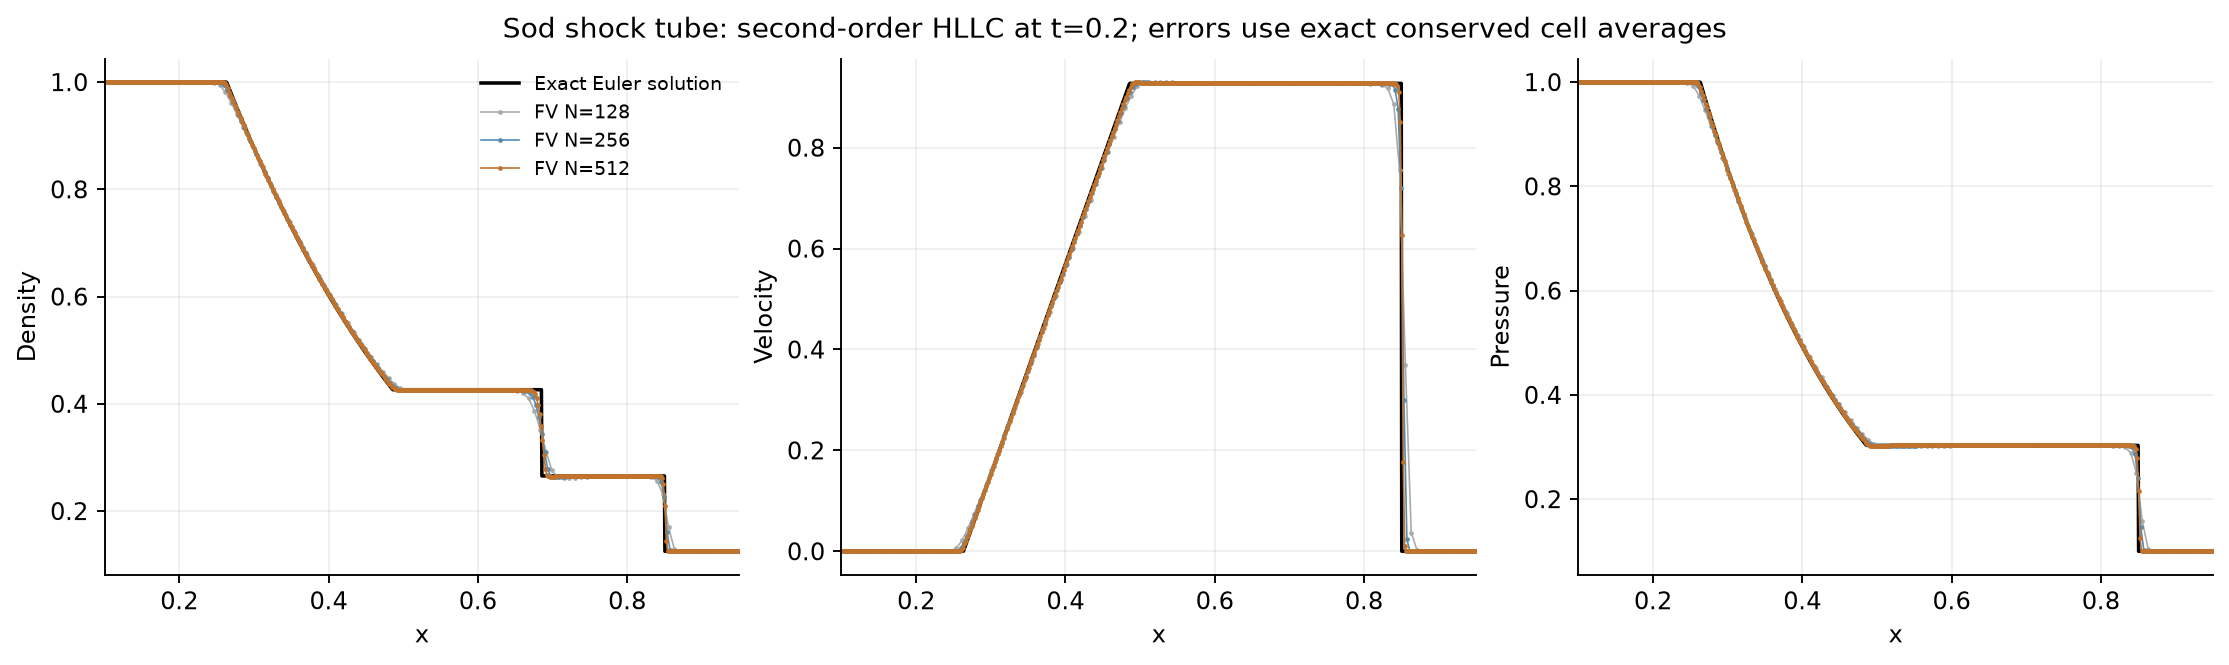
\includegraphics[width=\textwidth]{hydro_fv_sod}\\[2mm]
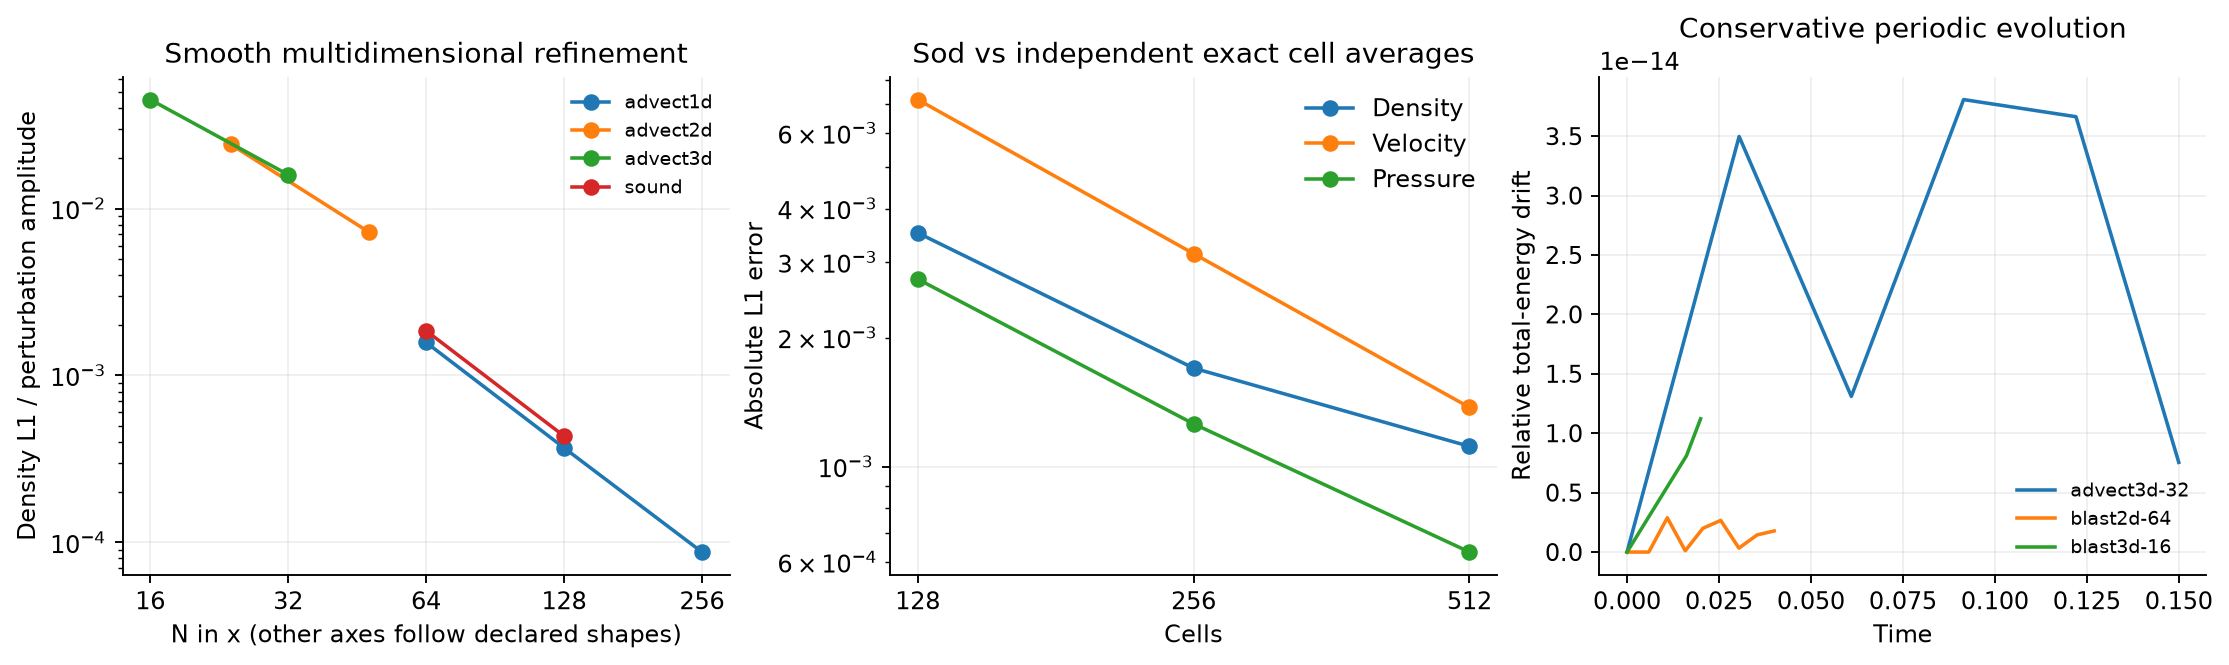
\includegraphics[width=\textwidth]{hydro_fv_convergence}
\caption{Finite-volume validation (\file{Hydrodynamics/tests/figures}). \emph{Top:} the Sod shock tube with second-order HLLC at
$t=0.2$ for 128, 256 and 512 cells against the exact Euler solution. \emph{Bottom:} convergence of smooth advection and sound waves in
1--3D, the Sod L1 errors against exact cell averages, and the relative drift of the total energy in periodic runs ($\lesssim4\times10^{-14}$).}
\label{fig:hydro-fv}
\end{figure}


\section{Smoothed-particle hydrodynamics}\label{sec:hydro-sph}

\cls{Solver} evolves periodic gas particles in 1D/2D/3D with the variational density--energy formulation summarised by
Price \cite{Price2012}. The kernel is the cubic B-spline $W=\sigma_Dh^{-D}f(r/h)$ with support $2h$,
$f=1-\frac32q^2+\frac34q^3$ for $q<1$ and $\frac14(2-q)^3$ for $1\le q<2$ ($\sigma_D=\frac23,\frac{10}{7\pi},\frac1\pi$).
Each particle solves for its smoothing length and density together, and the forces follow from the Lagrangian:
\begin{gather}
\rho_i=\sum_jm_jW(r_{ij},h_i),\qquad h_i^D\rho_i=\eta^Dm_i,\qquad
\Omega_i=1+\frac{h_i}{D\rho_i}\sum_jm_j\frac{\partial W(r_{ij},h_i)}{\partial h_i},\\
\frac{\dd\bm v_i}{\dd t}=-\sum_jm_j\left[\frac{P_i}{\Omega_i\rho_i^2}\nabla_iW(h_i)+\frac{P_j}{\Omega_j\rho_j^2}\nabla_iW(h_j)
+\Pi_{ij}\nabla_i\bar W\right],\\
\frac{\dd u_i}{\dd t}=\sum_jm_j\left[\frac{P_i}{\Omega_i\rho_i^2}\bm v_{ij}\cdot\nabla_iW(h_i)+\tfrac12\Pi_{ij}\bm v_{ij}\cdot\nabla_i\bar W\right].
\end{gather}
The $\Omega$ (grad-$h$) terms make the equations exactly conservative; force searches use the union of both particles'
supports. The $(h,\rho)$ root is found by bracketed Newton/bisection within $[h_{\min},h_{\max}]$ (a failure is a
collective error, never a silent clamp).

\paragraph*{Dissipation.} Artificial viscosity for approaching pairs,
$\mu_{ij}=\bar h\,\bm v_{ij}\cdot\bm r_{ij}/(r^2+\epsilon\bar h^2)$,
$\Pi_{ij}=(-\alpha\bar c\mu_{ij}+\beta\mu_{ij}^2)/\bar\rho$ (default $\alpha=1$, $\beta=2$), with the Balsara shear limiter
$|\nabla\cdot\bm v|/(|\nabla\cdot\bm v|+|\nabla\times\bm v|+\epsilon c/h)$ \cite{Balsara1995}; optional artificial
conductivity $\alpha_u\sum_jm_j(u_i-u_j)\sqrt{|P_i-P_j|/\bar\rho}\,\bar W'/\bar\rho$.

\paragraph*{Time integration and cosmology.} A global time step (Courant, acceleration and energy-change limits) with
Heun RK2; a failed step restores the particles. An \code{ExternalForce} callback adds gravity. With a prescribed 3D
background, positions and $h$ are comoving and
\begin{equation}
\frac{\dd\vx}{\dd t}=\frac{\bm v}{a},\qquad
\frac{\dd\bm v}{\dd t}=\frac{\bm a_{\rm hydro}}{a}-H\bm v+\bm g,\qquad
\frac{\dd u}{\dd t}=\frac{\dot u_{\rm hydro}}{a}-3(\gamma-1)Hu,
\end{equation}
with the physical relative velocity $\bm v_{ij}+aH\bm x_{ij}$ in the viscosity. MPI uses the $x$ slabs of \fml{} with
ghost exchanges within $2h_{\max}$ for densities and twice the largest $h$ for forces.

\begin{validation}[Validation: SPH (\file{SPH/tests/RESULTS.md})]
Densities, $\Omega$, forces and heating against all-pair sums ($10^{-15}$); total momentum and energy rates conserved to
$10^{-16}$; the forces equal the fixed-entropy derivative of the internal energy ($2\times10^{-10}$); sound waves
converge at second order in 1D; Sod shock tube L1 density errors $0.017$, $0.009$, $0.005$ for 225, 450, 900 particles
with gas-energy drift $\sim10^{-6}$; uniform expansion reproduces $v\propto a^{-1}$ and $u\propto a^{-2}$; identical results on
1, 2 and 4 ranks.
\end{validation}

\begin{figure}[htbp]
\centering
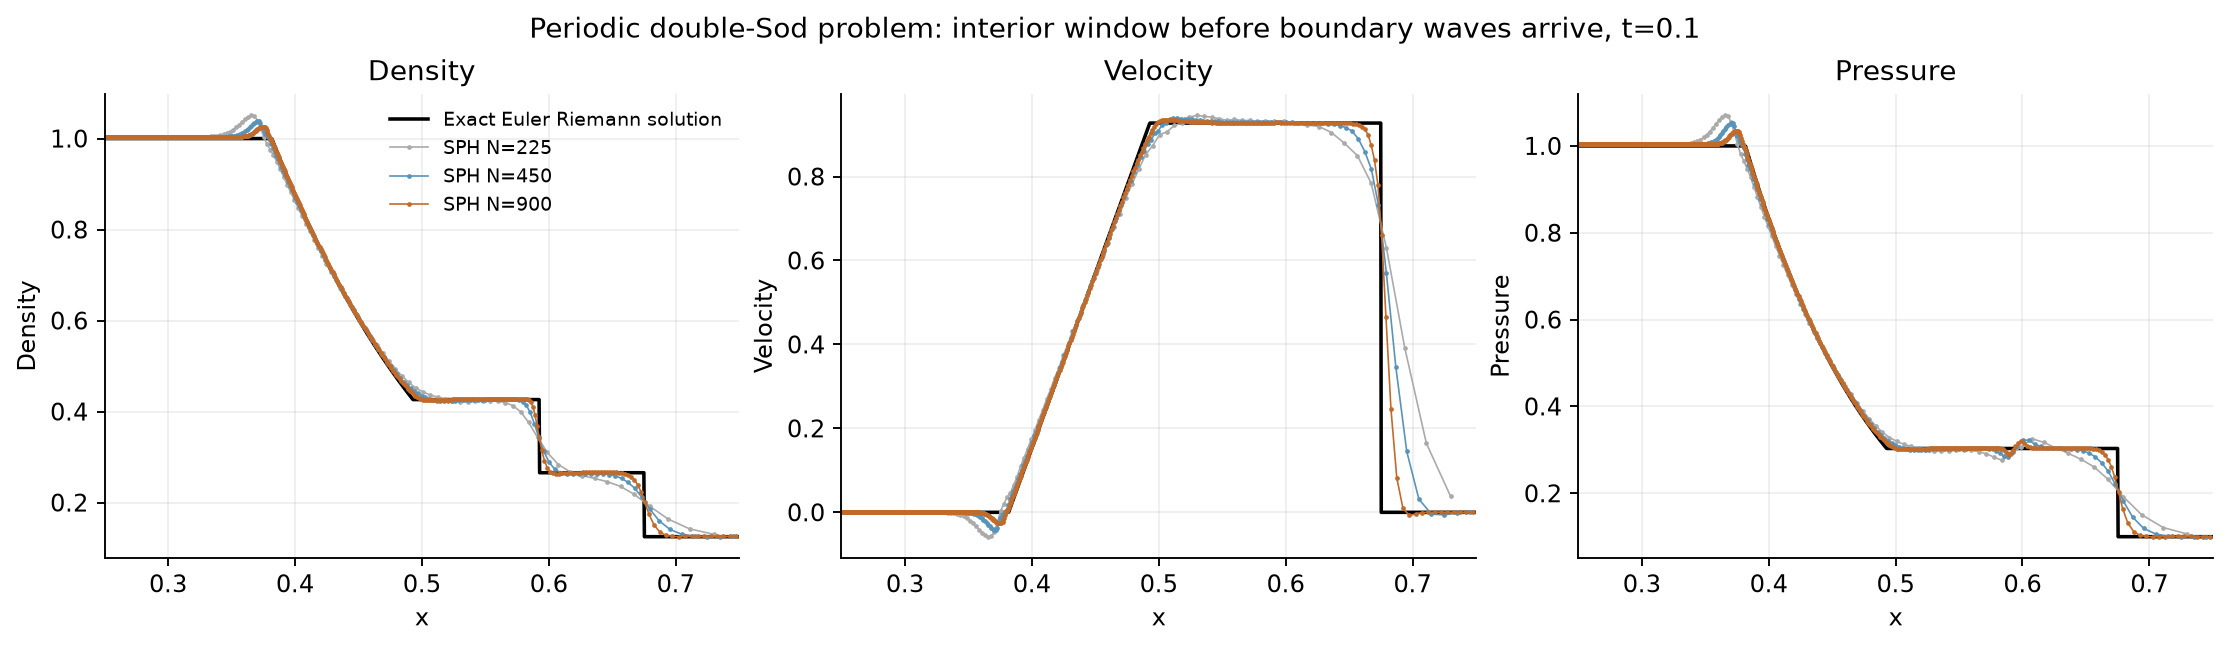
\includegraphics[width=\textwidth]{sph_sod}
\caption{SPH on the periodic double-Sod problem at $t=0.1$ for 225, 450 and 900 particles against the exact Riemann solution
(\file{SPH/tests/figures}): the blips at the contact discontinuity and the smoothed shock are the usual SPH behaviour and shrink with
resolution.}
\label{fig:sph-sod}
\end{figure}


\section{Wave dark matter}\label{sec:wavedm}

Ultralight bosons of mass $m$ ($\sim10^{-22}$\,eV) have a de Broglie wavelength of astrophysical size and are described
by a classical wave obeying the Schr\"odinger--Poisson equations \cite{Hu2000FDM,Schive2014}. With $\eta=\hbar/m$ and the
comoving wavefunction $\psi$ (the homogeneous $a^{-3/2}$ dilution absorbed), $\rho_{\rm com}=|\psi|^2$ and $U=a\Phi$,
\begin{equation}
i\frac{\partial\psi}{\partial t}=-\frac{\eta}{2a^2}\nabla^2\psi+\frac{U}{\eta a}\psi,\qquad
\nabla^2U=4\pi G\left(\rho_{\rm com}+\rho_{\rm ext}-\bar\rho_{\rm tot}\right),
\end{equation}
in cosmic time, for one non-relativistic species without self-interaction. \code{Physics::from_si(m_eV, L0, T0, M0)}
converts to code units ($\eta=(\hbar/m)T_0/L_0^2$, $G=G_{\rm SI}M_0T_0^2/L_0^3$).

\paragraph*{Split-step method.} The wavefunction lives on a full complex grid (\cls{CFFTWGrid} slabs or
\cls{CPencilGrid} pencils; all $N^3$ modes are independent). A step is the kick--drift--kick split
\begin{equation}
\psi\leftarrow e^{-iU_{\rm init}B/(2\eta)}\psi,\qquad
\psi_{\vk}\leftarrow e^{-i\eta k^2A/2}\psi_{\vk},\qquad
\psi\leftarrow e^{-iU_{\rm final}B/(2\eta)}\psi,\qquad A=\int\frac{\dd t}{a^2},\quad B=\int\frac{\dd t}{a},
\end{equation}
with the potential recomputed from the density after the kinetic substep (the potential substeps preserve the
density exactly). At fixed $a$ this is the second-order Strang split; with the integrated factors it is second order for
a smooth prescribed expansion. \code{step_scale_factor(a_next, H)} computes $\dd t=\int\dd a/(aH)$, $A$ and $B$ by
Gauss--Legendre quadrature. The kinetic phase is a product of three tabulated 1D factors; a self-gravitating step costs
four complex FFTs. \code{suggested_timestep} bounds the kinetic and potential phases per step. No norm repair or high-$k$
filtering is applied.

\paragraph*{Initial conditions and coupling.} \code{initialize(field)}, \code{initialize_density_phase(rho, theta)}
($\psi=\sqrt\rho\,e^{i\theta}$) or \code{initialize_density_velocity_potential(rho, sigma)} ($\theta=a\sigma/\eta$ for
$\bm u=\nabla\sigma$, single stream). An external comoving density (e.g.\ CDM particles) can source the potential
(\code{set_external_density}), and \code{gravity_acceleration} returns $-\nabla U/a^3$ for particles.

\paragraph*{Energy diagnostics.} $K=\frac{\eta^2}{2a^2}\int|\nabla\psi|^2$, $W=\frac{1}{2a}\int\rho U$; in an expanding
background $\dd E/\dd t=-H(2K+W)$, and \cls{EnergyBalance} tracks the residual
$E(a)-E(a_0)+\int(2K+W)\,\dd\ln a$.

\begin{cppcode}[A wave dark matter run]
#include <FML/WaveDarkMatter/SchrodingerPoisson.h>
using namespace FML::WAVEDM;
auto physics = Physics::from_si(1e-22, FML::UTILS::SI::kpc, FML::UTILS::SI::Gyr, 1e7 * FML::UTILS::SI::Msun);
Solver solver(64, 20.0, physics);                  // 64^3, box of 20 code lengths
solver.initialize_density_phase([](auto x) { return 1.0 + 0.01 * std::cos(2 * M_PI * x[0] / 20.0); },
                                [](auto) { return 0.0; });
solver.step(1e-3);                                 // fixed a; or step_scale_factor(a_next, H)
auto d = solver.diagnostics();                     // mass, K, W, high-k tail fraction
\end{cppcode}

\begin{validation}[Validation: wave dark matter (\file{WaveDarkMatter/tests/RESULTS.md})]
Complex FFTs against explicit DFTs; free-wave dispersion, interference, Parseval, Poisson signs; a nonlinear $4^3$
field against an adaptive DOP853 method-of-lines reference; second-order convergence in $\Delta t$ (field errors
$1.7\times10^{-3}$, $4.3\times10^{-4}$, $1.1\times10^{-4}$ for $\Delta t=0.1$, $0.05$, $0.025$); a soliton from an
independent boundary-value solution stays stationary (relative static-energy drift $5\times10^{-8}$); slabs and
pencils agree to $10^{-14}$; versioned checksummed checkpoints restart with a different number of tasks.
\end{validation}

\chapter{Potential gradient descent and baryonification}\label{ch:pgd-baryonification}
\chapterstatus{written}{2026-11-20}

Two post-processing methods move the particles of a gravity-only simulation to mimic physics it does not resolve or
contain: potential gradient descent (PGD) sharpens the haloes of low-resolution PM simulations, and baryonification
displaces particles around haloes to mimic the effect of gas, stars and feedback on the matter distribution.

\begin{modulebox}{PGD and Baryonification}
\file{PGD/PotentialGradientDecent.h} (example \file{PGD/example}); \file{Baryonification/Baryonification.h},
\file{Baryonification/Profiles.h} (namespace \nsp{FML::BARYONIFICATION}); SimulationCode integration
\file{src/BaryonificationOutput.h/.cpp}.\par
Documentation: \file{Baryonification/README.md}, \file{SimulationCode/ANALYSIS.md}.
\end{modulebox}

\section{Potential gradient descent}\label{sec:pgd}

PM simulations with few steps and coarse force grids produce haloes that are too extended. Dai, Feng and Seljak
\cite{Dai2018PGD} move the particles a little further down the gradient of a band-pass filtered potential:
\begin{equation}
\bm S=-\alpha\,\mathcal N\,\nabla\,\hat O_l\hat O_s\nabla^{-2}\delta,\qquad
\hat O_l=e^{-k_l^2/k^2},\qquad \hat O_s=e^{-k^4/k_s^4},
\end{equation}
where $\hat O_l$ removes the large scales (which the PM simulation gets right) and $\hat O_s$ the scales below the
resolution. With the paper's definition of the fitted, dimensionless $\alpha(a)$ the prefactor is
$\mathcal N=4\pi G\bar\rho/H_0^2=\frac32\Om_m$ (with $\bar\rho$ the comoving mean density); a positive $\alpha$ moves
particles towards overdensities. The density is assigned to a grid, filtered and differentiated in Fourier space, and
the displacement interpolated back to the particles. The function is collective; the \cls{MPIParticles} overload
communicates the moved particles. Parameters: $k_l$, $k_s$ (in box units) and $\alpha$, calibrated by the paper's
fitting formulae (\code{pgd_fitting_formula_*}).

\section{Baryonification}\label{sec:baryonification}

\paragraph*{Model.} Following Schneider and Teyssier \cite{SchneiderTeyssier2015} and the profile family of
Schneider et al.\ \cite{Schneider2019}, each halo's gravity-only (reference) profile is replaced by a profile of
collisionless matter, gas and a central galaxy, and particles are displaced so that enclosed masses match. With
$x=r/R_{200}$:
\begin{itemize}
\item reference: a truncated NFW profile $\propto[cx(1+cx)^2(1+(x/\epsilon)^2)^2]^{-1}$, normalised to $M_{200}$;
\item gas: $\propto(1+x/\theta_{\rm co})^{-\beta}[1+(x/\theta_{\rm ej})^2]^{-(7-\beta)/2}$ with $\beta=3-(M_c/M_{200})^\mu$;
\item central galaxy: $\rho\propto r^{-2}\exp[-(r/2R_h)^2]$ (cumulative mass analytic with erf);
\item collisionless matter (dark matter and satellite stars), optionally relaxed by
      $r_f/r_i-1=A[(M_i/M_f)^n-1]$, $M_f=f_{\rm clm}M_i+M_{\rm gas}(r_f)+M_{\rm cga}(r_f)$ (bisection);
\item stellar fractions $f_\star=A_\star(M_1/M_{200})^{\eta}$, gas $f_b-f_\star$.
\end{itemize}
\paragraph*{Displacement.} With the cumulative masses $M_{\rm ref}(r)$ and $M_{\rm bar}(r)$, a particle at $r$ moves
radially to $r'$ with $M_{\rm bar}(r')=M_{\rm ref}(r)$ (\cls{RadialMapping} of monotone piecewise-linear tables). All
components are normalised at a finite support (default $30R_{200}$) with a uniform background, so the displacement
vanishes outside it; overlapping haloes add their displacement vectors, evaluated at the original positions. This is a
finite-support implementation of the profile family, not a reproduction of the paper's calibrated predictions; there is
no correlated two-halo term. Velocities, masses and IDs are unchanged.

\paragraph*{In SimulationCode.} \code{baryonification = true} runs the method at each output on a copy of the particles
(the live simulation is unchanged): FoF seeds, spherical-overdensity $M_{200c}$ and $R_{200c}$ with shrinking-sphere
centres, rejection of truncated, nested or unresolved hosts, a power-law concentration (illustrative, not fitted from PM
cores), and outputs of the corrected and original $P(k)$ and their ratio, the host catalogue and optionally the
displaced particles. Requires 3D GR, one CDM+baryon species and no massive neutrinos.

The parameters map onto the model above (\param{baryonification_model} \code{= schneider2019}, the only family; the
defaults are illustrative, not calibrated). Gas: $M_c$ (\param{baryonification_gas_mass_scale_msunh}), $\mu$
(\param{baryonification_gas_mass_exponent}), $\theta_{\rm co}$ and $\theta_{\rm ej}$ in units of $R_{200c}$
(\param{baryonification_gas_core_radius_over_r200}, \param{baryonification_gas_ejection_radius_over_r200}); the NFW
truncation $\epsilon$ (\param{baryonification_truncation_radius_over_r200}). Stars: $M_1$, $A_\star$, the exponents of the
total and central stellar fractions and $R_h/R_{200c}$ (\param{baryonification_stellar_mass_scale_msunh},
\param{baryonification_stellar_amplitude}, \param{baryonification_stellar_total_exponent},
\param{baryonification_stellar_central_exponent}, \param{baryonification_stellar_radius_over_r200}). Relaxation:
\param{baryonification_relax_collisionless} with $A$ and $n$ (\param{baryonification_relaxation_amplitude},
\param{baryonification_relaxation_exponent}). Concentration $c=c_0(M_{200c}/M_{\rm piv})^{\alpha}(1+z)^{\gamma}$
(\param{baryonification_concentration_norm}, \param{baryonification_concentration_pivot_mass_msunh},
\param{baryonification_concentration_mass_slope}, \param{baryonification_concentration_redshift_power}). Hosts: FoF seeds
with \param{baryonification_fof_linking_length}, \param{baryonification_fof_min_particles},
\param{baryonification_fof_nmesh_max} and \param{baryonification_fof_buffer_mpch} (larger than the halo radii), and
$M_{200c}\ge$\,\param{baryonification_min_halo_mass_msunh}. Tables: \param{baryonification_profile_radial_bins} radii from
\param{baryonification_min_radius_over_r200} to the support \param{baryonification_max_radius_over_r200} (less than half the
box). \param{baryonification_output_particles} writes the displaced particles as a separate snapshot.

\begin{cppcode}[Baryonifying a catalogue]
#include <FML/Baryonification/Baryonification.h>
using namespace FML::BARYONIFICATION;
HaloProperties halo{1e14, 0.7, 5.0};               // M200 [Msun/h], R200 [Mpc/h], concentration
ModelParameters model;
model.gas_mass_scale = 1e14;  model.gas_ejection_radius = 4.0;
auto profiles = make_halo_profiles(halo, model, /*mean_density=*/8.3e10);
std::vector<HaloDisplacement> halos{{{50.0, 50.0, 50.0}, profiles.mapping()}};
Baryonifier correction(std::move(halos), /*boxsize=*/100.0);
correction.apply(particles.data(), particles.size());   // positions only
\end{cppcode}

\begin{caveat}
Validate against a chosen hydrodynamical calibration, halo completeness, halo mass and concentration errors, snapshot
resolution, the support and the radial tables; no percent-level accuracy is claimed. The halo catalogue and prepared
mappings are replicated on every rank. With PM resolution, SO masses are biased low unless $R_{200}$ spans several force
cells (\cref{ch:simulation-code}).
\end{caveat}


\part{Identifying structures}
\chapter{Halo finding and merger histories}\label{ch:halo-finding}
\chapterstatus{written}{2026-11-14}

Halos are found with friends-of-friends (standard and relaxed), their spherical-overdensity properties measured around
the FoF centres, substructure resolved with a phase-space finder, and halos followed between snapshots by particle
overlap. All of them run in \file{SimulationCode} on the fly and in the snapshot analyser (\cref{ch:snapshot-analyzer})
through the analysis layer.

\begin{modulebox}{FriendsOfFriends, PhaseSpaceHaloFinder, HaloHistory}
\nsp{FML::FOF}: \file{FriendsOfFriends/FoF.h} (\code{FriendsOfFriends}), \file{FriendsOfFriends/FoFBinning.h}
(\cls{FoFHalo}), \file{FriendsOfFriends/FoFDomain.h}, \file{FriendsOfFriends/RelaxedFoF.h}
(\code{RelaxedFriendsOfFriends}), \file{FriendsOfFriends/SphericalOverdensity.h} (\code{SphericalOverdensity}).
\nsp{FML::PHASE_SPACE_HALOS}: \file{PhaseSpaceHaloFinder/PhaseSpaceHaloFinder.h} (\code{find}), \file{Distributed.h}
(\code{find_distributed}), \file{BindingPotential.h}, \file{Adapters.h}.
\nsp{FML::HALO_HISTORY}: \file{HaloHistory/HaloHistory.h} (\code{match}, \code{build}), \file{HaloHistory/CatalogueIO.h}.\par
Documentation: \file{FriendsOfFriends/RelaxedFoF.md}, \file{FriendsOfFriends/SphericalOverdensity.md},
\file{PhaseSpaceHaloFinder/README.md} and \file{tests/RESULTS.md}, \file{HaloHistory/README.md}.
Tests: \file{tests/test_fof.cpp}, \file{tests/test_fof_domain.cpp}, \file{tests/test_so.cpp}, \file{tests/test_so_multislab.cpp},
\file{FriendsOfFriends/tests}, \file{PhaseSpaceHaloFinder/tests}, \file{HaloHistory/tests}.
\end{modulebox}

\section{Friends-of-friends}\label{sec:halo-fof}

Two particles are friends if they are closer than $b\,\bar n^{-1/3}$, $b$ the linking length in units of the mean particle
separation (typically 0.2), and a group is a connected set of friends \cite{Davis1985}. The particles are binned to a grid of
cells larger than two linking lengths (at most about one particle per cell; the result does not depend on the grid), so only
$2^D$ neighbouring cells need to be searched, and groups are grown by recursively tagging the friends of friends. The particles
are sorted by one coordinate first (20--30\% faster).

\paragraph*{MPI.} Each task receives copies of the particles within a buffer of its slab (or pencil, \file{FoFDomain.h}, with up to 8
neighbours) from the neighbouring tasks, links its particles and the copies, and keeps the groups whose centre it owns; the FoF IDs of the
copies are sent back to their owners, and IDs are unique across tasks. The buffer must exceed the largest halo
(\param{fof_buffer_length_mpch}, default $3\Mpch$); groups that reach its edge are counted and reported, as they might be cut and found
twice. Tasks without particles take part normally.

\paragraph*{Halo properties.} The halo class is a template parameter: \cls{FoFHalo} accumulates the number of particles, the mass (sum
of \code{get_mass}), the centre of mass with periodic unwrapping, the mean velocity and the velocity dispersion; a derived class can bin
anything else. FoF IDs are stored in the particles if they have \code{set_fofid}.

\begin{cppcode}[FoF halos]
#include <FML/FriendsOfFriends/FoF.h>
std::vector<FML::FOF::FoFHalo<Particle, 3>> halos;
FML::FOF::FriendsOfFriends<Particle, 3>(part.get_particles_ptr(), part.get_npart(),
                                        0.2,      // linking length b
                                        20,       // minimum particles per halo
                                        true,     // periodic
                                        3.0 / Boxsize, halos);
\end{cppcode}

In \file{SimulationCode}: \param{fof}, \param{fof_linking_length}, \param{fof_nmin_per_halo}, \param{fof_buffer_length_mpch}, the
output format and the mass function binning. With separate CDM and baryon particles, linking lengths and particle counts refer to one
species.

\section{Relaxed FoF}\label{sec:halo-rfof}

In low-resolution (PM/COLA) simulations small halos are too diffuse for $b=0.2$ and fragment, so the mass function is too low and the
bias of small halos too high. The relaxed FoF of Dai et al.\ \cite{Dai2019} (as in FastPM \cite{Feng2016}) uses a longer linking length
for small halos and rejects unbound clumps joined by it through their velocity dispersion:
\begin{enumerate}
\item halos are binned by particle number with edges $N_i=20,40,80,160,320,\infty$;
\item the linking length of bin $i$ interpolates linearly between $\ell_1(z)=l_1-a_1/(1+z)$ for the smallest and
      $\ell_n(z)=\max[l_6-a_2/(1+z),\ell_{\min}]$ for the largest halos;
\item a halo is fake if $\sigma_v\ge r_0(z)V_{\rm std}(M,z)$, with the 3D dispersion $\sigma_v$, $r_0=b_1-b_2\ln(1+z)$ and
      $V_{\rm std}=V_0[E(z)M/10^{15}M_\odot h^{-1}]^{1/3}$, $V_0=1100$\,km/s \cite{Evrard2008};
\item pass $i$ runs FoF with $\ell_i$ on the remaining particles, saves the genuine groups smaller than $N_i$ (with at least
      \code{nmin} particles) and removes their particles and all ungrouped ones; the rest go to the next pass.
\end{enumerate}
The \code{fastpm} mode (default) stops after the $n$ passes; the \code{paper} mode continues with linking lengths shrinking by 0.9 per
pass and saves every group that passes the velocity cut (Algorithm 1 of the paper). The defaults are FastPM's
($l_1=0.25$, $a_1=0.012$, $l_6=0.24$, $a_2=0.06$, $\ell_{\min}=0.2$, $b_1=7.02$, $b_2=6.025$, $n_{\min}=8$), fitted to TNG300-2-Dark for
FastPM with a $0.3\Mpch$ mean separation and 40 steps; for other set-ups they should be refitted. $r_0(z)\le0$ for $z>2.2$, where every halo
would be rejected: the code warns and \code{r0_min} sets a floor. In \file{SimulationCode}: \param{fof_relaxed} and the
\code{fof_relaxed_*} parameters; the catalogue then has the pass, bin, linking length and $\sigma_v/V_{\rm std}$ of each halo.

\begin{validation}[Validation: FoF]
\file{tests/test_fof.cpp}: groups, centres and stored IDs equal a serial FoF for any number of tasks; buffer-edge groups are reported; custom
halo classes; the linking length in 2D. \file{tests/test_relaxed_fof.cpp} on 1, 2 and 4 tasks: members, pass, bin and size of every halo
equal an independent SciPy KD-tree implementation on a catalogue with compact, diffuse and fake clumps and cold cores in hot envelopes, in both
modes and at several redshifts; one bin without the velocity cut is standard FoF; tasks without particles.
\end{validation}

\section{Spherical overdensity}\label{sec:halo-so}

\code{SphericalOverdensity} measures halos around given centres (e.g.\ the FoF centres) using all particles, not only the group members:
\begin{enumerate}
\item the centre is refined by a shrinking sphere \cite{Power2003}: move to the centre of mass of the particles inside and shrink the radius by
      10\% until fewer than $\max(n_{\min},10\%)$ of the starting particles remain (at most 200 iterations);
\item for each threshold $\Delta$ (in units of the mean density) the radius is the \emph{outermost} radius where the mean enclosed density is
      still above $\Delta\bar\rho$: with the particles sorted by distance, the largest $i$ with $M_i/(\frac43\pi r_i^3)\ge\Delta\bar\rho$, and
      $R_\Delta$ from $M_i/(\frac43\pi R_\Delta^3)=\Delta\bar\rho$. Growing from the centre and stopping at the first crossing is not well
      defined at simulation resolution: the innermost particles are Poisson noise around a centre that is not on a particle;
\item mass-weighted mean velocity and dispersion inside the first radius.
\end{enumerate}
The definitions in \file{SimulationCode} (\param{fof_so_definitions}) are $\Delta$ times the mean (\code{200m}), the critical density
(\code{500c}) or the virial overdensity of Bryan and Norman (\code{vir}) \cite{BryanNorman1998}. The search radius is the same on all tasks
so results do not depend on the decomposition; particles come from every slab that intersects the search spheres, the buffer is refreshed
collectively if a centre moves, and halos whose sphere did not reach the threshold are flagged as truncated.

\begin{validation}[Validation: spherical overdensity]
Singular isothermal spheres on a uniform background (also on task boundaries) give the analytic radius, mass and centre for any number of
tasks; spheres beyond the search radius are flagged; cored halos of $\sim100$ particles (as in PM simulations) do not collapse to a few
particles. \file{tests/test_so_multislab.cpp}: exact ghost membership from non-adjacent slabs, variable-size records, bounded messages, empty
and non-uniform slabs, and a direct full-catalogue reference for centres, radii, masses, velocities and truncation.
\end{validation}

\section{Phase-space halos}\label{sec:halo-phasespace}

\file{PhaseSpaceHaloFinder} is an independent implementation of a hierarchical phase-space halo finder inspired by ROCKSTAR
\cite{Behroozi2013}:
\begin{itemize}
\item spatial FoF parents with linking parameter 0.28;
\item in each parent, positions and velocities normalised by the mass-weighted dispersions, a 6D FoF radius from the 70\% quantile of the
      nearest-neighbour distances, and recursive refinement into children down to a minimum core size;
\item the leaf groups seed halos; seeds consistent within the Poisson errors of their core positions and velocities are merged, and a sampled
      6D density-saddle test removes weaker peaks without a resolved dip towards a denser one;
\item particles are assigned on the way back up with a dynamical position scale from the seed's circular velocity and a reference density
      (200 times the mean by default);
\item unbinding with the full isolated Newtonian potential of the assigned halo (a monopole tree with opening angle 0.7, the spline-softened
      Green function of \cref{ch:short-range}, an optional Hubble-flow term), iterated until stable.
\end{itemize}
The output has exclusive bound memberships by particle ID, bound and inclusive masses, core position and velocity, dispersions,
$V_{\max}$ and $R_{\max}$, the bound extent (not an SO radius) and the host. It runs serially, with OpenMP and on MPI slabs: FoF chains across
any number of slabs are stitched by propagating minimum IDs to a fixed point, and complete parents are routed to a hash owner, without
gathering the catalogue. Adapters give seeds for the SO measurement, HOD halos and history snapshots. This is a first implementation, not a
calibrated ROCKSTAR replacement.

\begin{validation}[Validation: phase-space finder]
Exact potentials against direct sums; two overlapping populations separated in velocity are recovered; invariance under permutation, rotation,
boosts, translation and unit rescaling; Plummer spheres give one object with $V_{\max}$ within 1--4\% of the analytic value; identical serial
and distributed memberships. Planted subhalos on circular orbits in a Plummer host were recovered in 40 of 48 realisations (misses within
1.5--2.5 scale radii of the host centre). An isolated 4000-particle Plummer sphere gives $V_{\max}=97.10$\,km/s against ROCKSTAR's 97.05\,km/s and
a bound mass within 0.3\% of ROCKSTAR's $M_{200b}$ (\file{tests/RESULTS.md}).
\end{validation}

\section{Merger histories}\label{sec:halo-history}

\file{HaloHistory.h} links halo catalogues of successive snapshots by shared particle IDs \cite{Srisawat2013,Elahi2019}. For halos $a$ and $b$
with $N_a$, $N_b$ members of which $N_{ab}$ are shared, the merit is
\begin{equation}
\mathcal M_{ab}=\frac{N_{ab}^2}{N_aN_b}=\frac{N_{ab}}{N_a}\frac{N_{ab}}{N_b},
\end{equation}
and each halo's descendant is the candidate with the largest merit (then the most shared particles, then the smallest ID), above optional
thresholds; all candidates are kept for inspection. Sorted particle-ID indices are merge-joined, so only pairs that share a particle get a
counter. A target's main progenitor is chosen among the sources whose descendant it is. With a gap allowance a halo without a descendant is
matched to the earliest later snapshot where it reappears. Catalogues carry required metadata (mass definition, ID namespace, units) that must
agree, exclusive or inclusive membership, and an acyclic host forest; \file{CatalogueIO.h} reads and writes a versioned ASCII format and
converts to HOD halos. Matching two snapshots of $10^7$ halo particles in $10^5$ halos takes about 7\,s on one core. It is a baseline, not a
reproduction of TreeFrog, SubLink or Consistent Trees.

\chapter{Cosmic web, tidal fields and morphology}\label{ch:cosmic-web}
\chapterstatus{written}{2026-11-14}

The large-scale structure is classified into voids, sheets, filaments and knots from the eigenvalues of the tidal and
velocity-shear tensors (T-web, V-web) or from the stream crossings of the particles (ORIGAMI), and its morphology is measured
with Minkowski functionals of excursion sets.

\begin{modulebox}{CosmicWeb, TidalTensor, Morphology}
\nsp{FML::COSMICWEB}: \file{CosmicWeb/CosmicWeb.h} (\code{TWeb}, \code{VWeb}, \code{classify_tensor}, \cls{TWebOptions}),
\file{CosmicWeb/ORIGAMI.h} (\code{ORIGAMI}), \file{CosmicWeb/ORIGAMIHalos.h} (\code{ORIGAMIHalos}); \file{TidalTensor/Hessian.h}
(\code{ComputeHessianWithFT}, \code{SymmetricTensorEigensystem}); \nsp{FML::MORPHOLOGY}: \file{Morphology/VoxelMorphology.h}
(\code{excursions}, \code{measure}).\par
Documentation: \file{CosmicWeb/README.md}, \file{TidalTensor/Workspace.md}, \file{Morphology/README.md}. Tests:
\file{tests/test_cosmicweb.cpp}, \file{tests/test_cosmicweb_pencil.cpp}, \file{tests/test_reconstruction.cpp}, \file{Morphology/tests},
\file{tests/test_morphology_pencil.cpp}.
\end{modulebox}

\section{T-web and V-web}\label{sec:web-tweb}

The T-web \cite{Hahn2007,ForeroRomero2009} uses the tidal tensor of the (Gaussian-smoothed) density contrast,
\begin{equation}
T_{ij}=\partial_i\partial_j\phi,\qquad\nabla^2\phi=\delta,\qquad T_{ij}(\bm k)=\frac{k_ik_j}{k^2}\delta(\bm k),
\end{equation}
whose trace is $\delta$; the V-web \cite{Hoffman2012} the normalised velocity shear
\begin{equation}
\Sigma_{ij}=-\frac{\partial_iv_j+\partial_jv_i}{2H},
\end{equation}
e.g.\ from the DTFE velocity field (\cref{sec:voids-dtfe}). A cell is a void, sheet, filament or knot if 0, 1, 2 or 3 eigenvalues exceed the
threshold $\lambda_{\rm th}$ (positive values, $\sim0.1$--0.4, give visually better webs \cite{ForeroRomero2009,Hoffman2012}). The eigenvalues
of the symmetric $3\times3$ matrices are computed by cyclic Jacobi rotations, accurate also for (nearly) degenerate eigenvalues, without GSL.
The result holds the classification, optionally the eigenvalues, and the volume and mass fractions of each class; the labels can be stored as one
byte per cell (\code{ClassificationStorage::Bytes}: 1\,GiB instead of 8\,GiB at $1024^3$). \code{TWeb} also takes particles and assigns them to a
grid first. Slabs and pencils are supported.

\begin{cppcode}[T-web classification]
#include <FML/CosmicWeb/CosmicWeb.h>
using namespace FML::COSMICWEB;
TWebOptions opt;
opt.smoothing_scale  = 2.0 / Boxsize;     // Gaussian, box units
opt.lambda_threshold = 0.2;
opt.classification_storage = ClassificationStorage::Bytes;
CosmicWeb web;
TWeb(delta_real, opt, web);               // or TWeb(particles, NumPart, Nmesh, opt, web)
int type = web.get_classification({ix, iy, iz});   // 0 void, 1 sheet, 2 filament, 3 knot
\end{cppcode}

\file{TidalTensor/Hessian.h} computes Hessians of fields by FFT (all components from one retained Fourier copy) and their eigenvalues and
eigenvectors with GSL, for the tidal field and the shear used elsewhere (e.g.\ LPT, \cref{ch:lpt}).

\section{ORIGAMI}\label{sec:web-origami}

ORIGAMI \cite{Falck2012} classifies particles by the number of orthogonal axes along which their stream has crossed. Particles that started on a
lattice of $N^3$ points have crossed along a lattice row if their order along that direction is reversed; a particle is crossed along an axis if
it has crossed with any particle within a quarter of the row. Nine axes are checked ($x$, $y$, $z$ and the two diagonals in each coordinate
plane), grouped into four orthogonal triads, and the morphology is the largest number of crossed axes in one triad: 0 void, 1 wall, 2 filament,
3 halo. The lattice coordinate comes from the particle ID (the numbering of \code{create_particle_grid} and the initial conditions); with MPI the
rows are moved to the tasks as needed.

\code{ORIGAMIHalos} groups the halo particles on the Delaunay tessellation of all particles (\cref{sec:voids-dtfe}): Voronoi densities of all
particles, cores of Delaunay-connected halo particles above a density threshold, and the other halo particles attached in rounds to the halo of
their densest neighbour already in a halo (independent of order and number of tasks); groups without a core can be kept; no unbinding is done.

\section{Minkowski functionals}\label{sec:web-minkowski}

The morphology of an excursion set $\{\bm x:\delta(\bm x)\ge\nu\}$ is described by the four Minkowski functionals in 3D: volume, surface area,
integrated mean curvature and Euler characteristic \cite{SchmalzingBuchert1997}. \file{VoxelMorphology.h} computes them exactly for the union of
closed cubic voxels above the threshold by counting the occupied cubes $C$ and the unique faces $F$, edges $E$ and vertices $V$ of their cell
complex. With cell size $h$:
\begin{gather}
V_{\rm vol}=Ch^3,\qquad A=(2F-6C)h^2,\qquad\int H\,\dd A=\pi(3C-2F+E)h,\qquad\chi=V-E+F-C,
\end{gather}
and the conventional isotropic Crofton estimates of the underlying smooth field \cite{Schmalzing1999},
\begin{equation}
\left\{\frac{Ch^3}{L^3},\ \frac29\frac{(F-3C)h^2}{L^3},\ \frac29\frac{(E-2F+3C)h}{L^3},\ \frac{V-E+F-C}{L^3}\right\}.
\end{equation}
The two normalisations of area and curvature differ (the staircase area is $3/2$ of the Crofton one). Periodic or open boundaries are supported.
Each entity is counted exactly once by vertex-anchored patterns of the incident voxels, so the integer counts are exact across tasks and threads;
MPI exchanges one slice and reduces four counts.

\begin{validation}[Validation: cosmic web and morphology]
\file{tests/test_cosmicweb.cpp}: analytic tensors and thread-count consistency; \file{tests/test_cosmicweb_pencil.cpp}: slabs equal pencils.
Morphology: the counts against an explicit set-union enumeration; empty and full boxes, isolated cubes, face/edge/corner contacts, a cavity, a
periodic ring; uneven and empty slabs. For Gaussian random fields ($128^3$, smoothing of 4 cells, 4 realisations) the Crofton densities agree with
the continuum predictions \cite{SchmalzingBuchert1997} to $\sim1\%$ for $V_0$, $V_1$, 1--4\% for $V_2$ and 2--7\% for $V_3$ at $\nu=-2$--2, within
the statistical errors of 1--4\%.
\end{validation}

\chapter{Voids and tessellations}\label{ch:voids}
\chapterstatus{written}{2026-11-26}

The Delaunay tessellation of the particles gives density and velocity fields without a grid (DTFE) and the Voronoi densities of
watershed void finders. \fml{} has its own MPI-parallel Delaunay triangulation and periodic Voronoi tessellation in 2D and 3D, with
exact predicates and results that do not depend on the number of tasks, which can follow moving points (the building block of a
future moving-mesh hydro solver); the older tessellation uses CGAL. ZOBOV, the ORIGAMI halos and the DTFE run on either, the
native one by default; CGAL is optional. \fml{} has four void finders sharing one
catalogue format: spherical, voxel watershed (Revolver-like) and ZOBOV, with optional zone merging.

\begin{modulebox}{Triangulation, VoidFinders}
\nsp{FML::DELAUNAY} (header-only, no dependencies):
\file{Triangulation/Predicates.h}, \file{Delaunay.h} (\cls{Delaunay}), \file{PeriodicVoronoi.h} (\cls{PeriodicVoronoi}).
\nsp{FML::TRIANGULATION}: \file{Triangulation/VoronoiTessellation.h} (\cls{PeriodicVoronoiTessellation}, native),
\file{Triangulation/Watershed.h} (\code{WatershedOnGraph}), \file{Triangulation/PeriodicDelaunay.h} (\cls{MPIPeriodicDelaunay},
CGAL), \file{Triangulation/DTFE.h} (\cls{DTFE}, either), \file{Triangulation/WatershedBinning.h}. \file{VoidFinders/Void.h}
(\cls{Void}), \file{SphericalVoidFinder.h}, \file{VoxelVoidFinder.h} (also \code{VoxelWatershed}), \file{ZobovVoidFinder.h},
\file{ZoneMerging.h}.\par
Documentation: \file{Triangulation/DELAUNAY.md}, \file{Triangulation/README.md}, \file{VoidFinders/README.md}. Tests: \file{Triangulation/tests}
(\file{test_delaunay.cpp}, \file{test_delaunay_mpi.cpp}, \file{compare_cgal.cpp}, \file{compare_library.cpp}),
\file{tests/test_watershed_native.cpp}, \file{tests/test_origami_halos.cpp}, \file{tests/test_dtfe_native.cpp}, \file{VoidFinders/tests} (\file{test_spherical.cpp}),
\file{tests/test_delaunay_domain.cpp}, \file{tests/test_dtfe_pencil.cpp}, \file{tests/test_voids_pencil.cpp}. CGAL \cite{CGAL}
(\code{USE_CGAL}) is needed only for \cls{MPIPeriodicDelaunay} and the options that use it.
\end{modulebox}

\section{FML's own Delaunay triangulation}\label{sec:voids-native}

\paragraph*{Predicates.} Everything rests on two exact predicates, \code{orient} (the sign of
$\det[\bm p_1-\bm p_0,\dots,\bm p_D-\bm p_0]$) and \code{insphere} (+1 if $\bm q$ is inside the circumsphere of a positively
oriented simplex), with CGAL's conventions. The determinant is evaluated in floating point with Shewchuk's a priori error bound
\cite{Shewchuk1997} (times a safety factor 4); when the sign is uncertain it is recomputed exactly with floating-point expansions
of the input coordinates, with a fixed-size stack version when all coordinate differences are exact doubles (lattices, quantized
coordinates). The result is exact for any double input barring overflow.

\paragraph*{Triangulation.} \cls{Delaunay}$\langle D\rangle$ ($D=2,3$) uses incremental insertion \cite{Bowyer1981,Watson1981}, placing the points in Peano--Hilbert order into a super
simplex (Bowyer--Watson): a visibility walk from the last new simplex locates the point, a breadth-first search finds the cavity of
simplices whose circumspheres contain it, and the cavity is replaced by the simplices joining its boundary facets to the point.
Cospherical points (lattices) are resolved by the symbolic perturbation of Devillers \& Teillaud \cite{DevillersTeillaud2011},
as in CGAL: the result is the Delaunay triangulation of the points perturbed in the order of a per-vertex key, a valid and unique
Delaunay triangulation of the input. Duplicates are detected. \code{move(v, p)} moves a vertex (in place if its star stays valid
and locally Delaunay, otherwise by removal, filling the hole with the Delaunay triangulation of its link, and reinsertion).

\paragraph*{Periodic Voronoi tessellation with MPI.} \cls{PeriodicVoronoi}$\langle D\rangle$ is collective: each task gives its
points (any distribution: slabs, pencils, Peano--Hilbert ranges, random, empty tasks) and gets the Voronoi cells of its points
(volume, centroid) and every face touching them (area, centroid, normal, the neighbour's global id, task and index, the periodic
shift). Each task triangulates its points with \emph{ghosts}, copies of other tasks' points and periodic images: an initial
buffer of two mean spacings around the bounding box of its points, then rounds of \emph{certification}, in which the
circumsphere of every simplex with a local vertex is searched on every task (and image) whose bounding box it meets; the points
found are inserted, and a simplex that was searched and survives is final. This needs no assumption on how the points are
distributed and is exact. Coordinates are quantized to $2^{-40}$ of the box so that images are exact translates, perturbation keys
are (global id, image shift), and circumcentres, face rings and sums are computed in an order fixed by the keys, so the cells and
faces are \emph{bitwise identical for any number of tasks and any distribution}, and a face shared by two tasks is identical on
both (a flux can be computed once). The geometry is computed with OpenMP.

\paragraph*{Moving points.} \code{update(new_points)} gives exactly (bitwise) what a new tessellation of the new positions gives,
reusing the ghosts and the triangulation: the ghosts follow their points, points may cross the box and other tasks' bounding boxes
(positions carry a wrap count), and the simplices are certified again. \code{update_method = Automatic} chooses from sampled costs
between moving the vertices and retriangulating; it pays off when few points move (with 1\% of $2\times10^5$ points moving the
triangulation takes 0.39\,s instead of 1.71\,s); when all points move by more than $\sim1\%$ of the spacing an update costs about
as much as a build. The geometry is still recomputed in full.

\begin{cppcode}[Periodic Voronoi tessellation with MPI]
#include <FML/Triangulation/PeriodicVoronoi.h>
using namespace FML::DELAUNAY;
std::vector<std::array<double, 3>> points = ...;  // this task's points in [0, L)^3
PeriodicVoronoi<3> voronoi(points, L);            // collective
for (size_t i = 0; i < voronoi.ncells(); i++) {
    const auto & cell = voronoi.cells()[i];       // cell.id, cell.volume, cell.centroid
    auto [begin, end] = voronoi.cell_faces(i);    // codes of the faces of cell i
    // faces()[code >= 0 ? code : -code - 1]: area, centroid, normal, neighbour, shift, tasks
}
voronoi.update(new_points);                       // = a new build, reusing ghosts and triangulation
\end{cppcode}

\paragraph*{In the library.} \cls{PeriodicVoronoiTessellation}$\langle D\rangle$ (\file{Triangulation/VoronoiTessellation.h})
gives the tessellation in the form the library's users need: the Voronoi volume and the neighbours (Delaunay edges) of every local
particle, with neighbours on other tasks as boundary particles whose values are fetched from their owners. Unlike
\cls{MPIPeriodicDelaunay} there is no buffer or guard points to choose, the particles can be on any domain, and every local cell
is exact. \code{WatershedOnGraph} (\file{Triangulation/Watershed.h}) is the watershed on the neighbour graph of either
tessellation (steepest descent to a local minimum, ties broken by position, links between basins at the lowest connecting
value), \code{WatershedDensityNative} the density watershed on the native one. ZOBOV (\code{ZobovOptions::tessellation =
Native}) and the ORIGAMI halos (\code{OrigamiHaloOptions::tessellation}, \cref{sec:web-origami}) use it by default in builds
without CGAL, as do the Analysis library (\code{zobov_tessellation}) and SnapshotAnalyzer.

\begin{validation}[Validation: native triangulation]
\file{test_delaunay} (69 checks): the predicates equal exact 128-bit integer determinants for $4\times10^5$ small-integer cases
(thousands exactly degenerate) and the filter agrees with exact evaluation on $10^5$ nearly degenerate configurations;
triangulations of random, clustered, lattice and duplicated points are valid and Delaunay (brute force: no vertex inside any
circumsphere); periodic volumes sum to the box to $10^{-15}$, cells close to $10^{-13}$, divergence-theorem volumes agree to
$10^{-12}$, lattices give cubes, results are translation and thread invariant; \code{move}, \code{retriangulate} and
\code{update} equal fresh triangulations. \file{test_delaunay_mpi} (69 checks on 1--4 tasks): slab, pencil, Peano--Hilbert, random
and last-task distributions give cells and faces bitwise identical to all points on task 0, also after updates with points
crossing task and box boundaries. \file{compare_cgal}: the Delaunay edges (with periodic offsets) are identical to CGAL~5.6's
periodic triangulations for $10^5$ and $10^6$ random and clustered points in 2D and 3D, and the triangulation is 1.5--4 times
faster (3D, $10^6$ points: 7.3\,s against 18.0\,s on one core). \file{tests/test_watershed_native} and
\file{tests/test_origami_halos}: native Voronoi volumes, basins, links, ZOBOV catalogues and ORIGAMI halos are independent of how
the particles are spread over the tasks and identical to CGAL's in 2D and 3D. \file{compare_library}: volumes, neighbour graph
and DTFE vertex densities against \cls{MPIPeriodicDelaunay}. \file{tests/test_dtfe_native}: native DTFE grids independent of the particle distribution (slabs, round robin, pencils) and equal
to CGAL's to $5\times10^{-12}$. On a $128^3$ COLA snapshot (200\,Mpc$/h$, $z=0$) the native tessellation gives the same ZOBOV voids
(8129), ORIGAMI halos (5148, every particle in the same halo) and DTFE grids (to $10^{-10}$) as CGAL on 1, 2 and 4 tasks, 1.2--3 times
faster, with a peak memory of 0.88 against 1.10\,GB per task on 4 tasks (2.66 against 2.06\,GB on one task).
\end{validation}

\begin{planned}[Planned]
Next for the moving mesh: recomputing only the geometry around moved points, and load balancing.
\end{planned}

\section{Periodic Delaunay tessellation with CGAL and the DTFE}\label{sec:voids-dtfe}

The DTFE (\cls{DTFE}, \code{DTFETessellation}) uses \fml{}'s own tessellation by default: the particles can be on any task, and the
triangulation is made exact over the grid cells each task fills; \code{DTFETessellation::CGAL} uses \cls{MPIPeriodicDelaunay} instead.
\cls{MPIPeriodicDelaunay} builds the 3D Delaunay tessellation of particles spread over the tasks with CGAL: each task triangulates its
particles plus a buffer from the neighbours (on the domain of the particles, slabs or pencils: the one given to the constructor or the
default particle domain; \cref{sec:par-communication}), and cells whose tetrahedra might be affected by the
buffer edge are flagged as unreliable. Voronoi volumes are the volumes of the contiguous Voronoi cells.

The Delaunay tessellation field estimator \cite{Schaap2000,Cautun2011} assigns each particle the density
\begin{equation}
\rho_i=\frac{(D+1)\,m_i}{W_i},
\end{equation}
with $W_i$ the volume of all tetrahedra sharing the particle, and interpolates any quantity known at the particles linearly inside each
tetrahedron, so gradients are constant per tetrahedron and the density integrates exactly to the total mass. Grid values are the field at the grid
point or the average over the cell ($n_{\rm sub}^3$ samples, volume- or mass-weighted). For velocities the DTFE gives the velocity, divergence,
vorticity and shear grids, the input of the V-web (\cref{sec:web-tweb}). Densities are in units of the mean; positions in $[0,1)$.

\begin{cppcode}[DTFE density and velocity fields]
#include <FML/Triangulation/DTFE.h>
FML::TRIANGULATION::DTFE<Particle> dtfe;
dtfe.create(part.get_particles_ptr(), part.get_npart());
FML::GRID::FFTWGrid<3> density;
dtfe.density_to_grid(Nmesh, density);                    // 1 + delta
FML::TRIANGULATION::DTFEVelocityGrids vel;
dtfe.velocity_to_grid(part.get_particles_ptr(), Nmesh, vel);   // divergence, vorticity, shear
\end{cppcode}

\section{Void finders}\label{sec:voids-finders}

All finders take particles with wrapped positions owned by their slab and return a catalogue of \cls{Void}s that is the same on every task: centre
(circumcentre of the minimum and its three lowest-density mutually adjacent neighbours for ZOBOV, the minimum for voxels), barycentre, volume,
effective radius $R=(3V/4\pi)^{1/3}$, minimum and mean density, the significance (the density at which the void links to a neighbour divided by its
minimum, ZOBOV's density ratio), membership counts, the merging hierarchy, and $\lambda=\delta_{\rm avg}R^{1.2}$ \cite{Nadathur2019}. Each can also
find overdense ``clusters'' by running on $1/\rho$.
\begin{itemize}
\item \emph{Spherical} \cite{Padilla2005}: underdense candidates on a density grid are grown to the largest sphere with mean density below
      $(1+\Delta)\bar\rho$, optionally recentred, and overlapping spheres removed in descending radius (\code{max_overlap}). Each task gets the
      particles within the search radius from every slab that needs them.
\item \emph{Voxel} (Revolver \cite{Nadathur2019}): a watershed of a smoothed CIC density grid; \code{VoxelWatershed} works on any density grid, e.g.\
      the DTFE's.
\item \emph{ZOBOV} \cite{Neyrinck2008}: the watershed of the Voronoi densities of the particles; zones are the basins of local minima.
      \code{ZobovOptions::tessellation} selects the native tessellation (\code{Native}, the default) or CGAL's
      (\code{CGAL}); both give the same catalogue.
\item \emph{Zone merging}: \code{None} (every zone is a void, as Revolver), \code{Threshold} (merge through links below $0.2\bar\rho$, as VIDE
      \cite{Sutter2015}) or \code{Full} (the ZOBOV hierarchy with parents).
\end{itemize}
The default grid (\code{Nmesh = 0}) is Revolver's, $\lfloor2(4\pi N/3)^{1/3}\rfloor$ rounded to a multiple of 8 (32 above 256), independent of the
number of tasks; for a given grid the spherical and voxel catalogues are identical for any number of tasks, and ZOBOV's does not depend on a grid.

\begin{validation}[Validation: tessellations and voids]
\file{tests/test_delaunay_domain.cpp}: on slabs and every pencil layout the same Voronoi volumes, no unreliable cells, and the same watershed basins;
\file{tests/test_dtfe_pencil.cpp}: DTFE densities, gradients and velocity fields on pencils equal those on slabs. \file{test_spherical.cpp}: exact ghost
IDs with tiny messages, periodic and slab boundaries, buffers wider than a slab, empty and non-uniform slabs, and a brute-force catalogue reference (radii,
centres, masses, members, overlap removal); \file{tests/test_voids_pencil.cpp}: voxel and spherical catalogues on pencils equal those on slabs;
\file{tests/test_watershed_native.cpp}: ZOBOV on the native tessellation independent of the particle distribution and identical to CGAL's. The
voxel and merging code has no unit test of its own; it was checked against an independent watershed implementation.
\end{validation}


\part{Clustering statistics}
\chapter{Power spectra and polyspectra}\label{ch:power-spectra}
\chapterstatus{written}{2026-11-15}

Fourier-space statistics of particles and fields in periodic boxes: auto and cross power spectra, redshift-space
multipoles, the bispectrum and higher polyspectra with the shell-product method, and the hybrid Lagrangian-bias basis
spectra with their perturbation-theory predictions.

\begin{modulebox}{ComputePowerSpectra}
\nsp{FML::CORRELATIONFUNCTIONS}: \file{ComputePowerSpectra/ComputePowerSpectrum.h} (\code{compute_power_spectrum},
\code{bin_up_power_spectrum}, \code{bin_up_cross_power_spectrum}, \code{compute_power_spectrum_multipoles},
\code{compute_bispectrum}, \code{compute_polyspectrum}, \ldots), \file{PowerSpectrumBinning.h} (\cls{PowerSpectrumBinning}),
\file{PolyspectrumBinning.h} (\cls{PolyspectrumBinning}, \cls{SparsePolyspectrumBinning}), \file{PolyspectrumWorkspace.h};
\nsp{HYBRIDBIAS}: \file{HybridBiasSpectra.h}, \file{HybridBiasOperators.h}, \file{HybridBiasZeldovich.h},
\file{HybridBiasOneLoop.h}, \file{HybridBiasOneLoopMG.h}, \file{HybridBiasLinearFieldIO.h}.\par
Documentation: \file{ComputePowerSpectra/README.md}. Tests: \file{tests/test_pofk.cpp}, \file{tests/test_spectra_pencil.cpp},
\file{tests/test_hybridbias.cpp}, \file{tests/test_hybridbias_pencil.cpp}.
\end{modulebox}

\section{The power spectrum estimator}\label{sec:pk-estimator}

From particles, \code{compute_power_spectrum} assigns them to a grid (\cref{ch:mass-assignment}), Fourier transforms, deconvolves the
window and bins
\begin{equation}
\hat P(k)=\frac{B^D}{N_k}\sum_{|\bm k|\in{\rm bin}}\frac{|\delta_{\bm k}|^2}{\tilde W^2(\bm k)}-P_{\rm shot},\qquad
P_{\rm shot}=B^D\frac{\sum_im_i^2}{(\sum_im_i)^2},
\end{equation}
with $N_k$ the number of modes in the bin (each r2c mode counted with its multiplicity) and $P_{\rm shot}=B^D/N$ for equal masses ($\sum w_i^2/N^2$ for
$\delta f$ particles). Interlacing (\cref{sec:ma-interlacing}) removes the leading aliasing, so with PCS or PQS the estimate is accurate close to the
Nyquist frequency on a smaller grid \cite{Sefusatti2016}. On a Fourier grid, \code{bin_up_power_spectrum}, \code{bin_up_cross_power_spectrum} and
\code{bin_up_deconvolved_power_spectrum} bin directly. \cls{PowerSpectrumBinning} holds linear or logarithmic bins between $k_{\min}$ and $k_{\max}$,
the mean $k$, the counts and the power; results are in box units until \code{scale(boxsize)} ($k\to k/B$, $P\to B^DP$); binnings can be combined
over realisations. A brute-force direct summation over particles and modes (no aliasing) is available for testing.

\begin{cppcode}[P(k) of particles]
#include <FML/ComputePowerSpectra/ComputePowerSpectrum.h>
using namespace FML::CORRELATIONFUNCTIONS;
PowerSpectrumBinning<3> pofk(kmin * Boxsize, kmax * Boxsize, nbins, PowerSpectrumBinning<3>::LINEAR_SPACING);
compute_power_spectrum<3>(Nmesh, part.get_particles_ptr(), part.get_npart(), part.get_npart_total(),
                          pofk, "PCS", /*interlacing*/ true);
pofk.scale(Boxsize);                         // h/Mpc and (Mpc/h)^3
\end{cppcode}

\section{Multipoles}\label{sec:pk-multipoles}

In the plane-parallel limit with line of sight $\hat{\bm n}$ and $\mu=\hat{\bm k}\cdot\hat{\bm n}$,
\begin{equation}
\hat P_\ell(k)=\frac{2\ell+1}{N_k}\sum_{|\bm k|\in{\rm bin}}|\delta_{\bm k}|^2\mathcal L_\ell(\mu),
\end{equation}
binned from the moments $\mu^{2n}|\delta_{\bm k}|^2$ (\code{compute_power_spectrum_multipoles_fourier}). From particles,
\code{compute_power_spectrum_multipoles} moves them to redshift space along each coordinate axis in turn,
$\bm x\to\bm x+\bm v\cdot\hat{\bm n}\,\hat{\bm n}/(aH)$ (the conversion factor depends on the velocity convention), and averages the three
estimates; the shot noise is subtracted from the monopole. In \file{SimulationCode}: \param{pofk_multipole} and its options, up to
\param{pofk_multipole_ellmax}.

\section{Polyspectra}\label{sec:pk-polyspectra}

The bispectrum and higher orders use the shell-product (FFT) method \cite{Scoccimarro2015}: for each $k$-shell $s$ the field
$\delta_s(\bm x)=\mathcal F^{-1}[\delta_{\bm k}\Theta_s(\bm k)]$ and the indicator $I_s(\bm x)=\mathcal F^{-1}[\Theta_s(\bm k)]$ are made, and
\begin{equation}
\hat B(k_1,k_2,k_3)=\frac{\sum_{\bm x}\delta_{s_1}\delta_{s_2}\delta_{s_3}}{\sum_{\bm x}I_{s_1}I_{s_2}I_{s_3}},
\end{equation}
the denominator counting the closed triangles $\bm k_1+\bm k_2+\bm k_3=0$ in the bins (the same for any order). The constant shot-noise terms are
subtracted for the power spectrum and bispectrum ($S_2$, $S_3=\sum m_i^3/(\sum m_i)^3$); the fourth order is the raw fourth moment, without the
disconnected Gaussian part.
\begin{itemize}
\item \emph{De-aliasing} (default): configurations must close as integer wave-vectors, not modulo the mesh; when a product could wrap, the shell fields
      are made on a padded mesh ($\times3.375$ cells for the bispectrum at the full Nyquist range, $\times8$ for the fourth order), and the ambiguous
      even-mesh Nyquist planes are excluded. \code{dealias = false} gives the previous modulo-grid estimator.
\item \emph{Caching}: the geometry counts are cached for reuse with the same mesh, edges and selection; shells are kept in a least-recently-used cache
      bounded by a number of shells or a memory budget (rebuilding evicted shells on demand), with the same schedule on all tasks.
\item \emph{Selected configurations} and \emph{sparse results} (\cls{SparseBispectrumBinning}, \ldots) store only the requested canonical
      configurations instead of $n_{\rm bins}^{\rm ORDER}$ values (e.g.\ 1.5\,GiB per task for 100 fourth-order bins); permutation-aware lookup.
\item A per-component report of the evaluation storage (input, results, shells, padding, remapping, reductions).
\item \emph{Shell overlap weights} (\code{shell_overlap_weights}, off by default; the global
      \code{polyspectrum_shell_overlap_weights_default} sets it for new binnings): each Fourier cell is weighted by the
      exact fraction of its volume inside the shell $[k_{\rm low},k_{\rm high})$ instead of 0 or 1 from its centre
      (``shell anti-aliasing'' as in CONCEPT, \arxiv{2112.01508}, whose closed-form overlap of a cell and a ball is ported in
      \file{ShellOverlap.h}). The weights enter the shell fields, the counts and the mean $k$ of the bins. The shells are
      then continuous: the mean $k$ of a bin moves smoothly with its edges, and for equilateral bins one cell wide the
      count follows the continuum $8\pi^2k^3\Delta k^3$ (in units of the fundamental mode) to better than 1\% from $k=3k_f$,
      where 0/1 shells scatter by 10--30\%. This helps comparisons with bin-averaged theory at low $k$ and for thin bins;
      it does not reduce the statistical errors, and neighbouring bins share their boundary cells. About 10\% more
      time for a $128^3$ bispectrum.
\end{itemize}
In \file{SimulationCode}: \param{bispectrum}, \param{bispectrum_nmesh}, \param{bispectrum_nbins},
\param{bispectrum_shell_overlap_weights} and the assignment options.

\begin{validation}[Validation: spectra]
\file{tests/test_pofk.cpp}: the shot noise for masses and $\delta f$ weights (exact, and Poisson particles give $P-P_{\rm shot}\approx0$), mass
conservation with interlacing, the triangle counts against a brute-force count, closure of high-frequency triangles as integer vectors, even and odd
meshes, the monopole equal to $P(k)$, and empty bins; for the shell overlap weights the exact cube--ball overlaps (the ball minus six caps), the
cells adding up to the ball, the weights of a cell summing to 1 over the bins, and the counts and the bispectrum of a random field equal to brute-force
weighted sums over the triangles. \file{tests/test_spectra_pencil.cpp}: mono-, bi- and trispectra with and without padding (and the bispectrum with
overlap weights) equal on slabs and every pencil layout. Primordial non-Gaussianity tests use the bispectrum of $f_{\rm NL}$ fields (\cref{sec:rf-fnl}).
\end{validation}

\section{Hybrid bias spectra}\label{sec:pk-hybrid}

In the hybrid Lagrangian bias model \cite{Modi2020,Kokron2021,Zennaro2023} the tracer field is a sum of Lagrangian operators advected with the
simulation particles,
\begin{equation}
\delta_t(\bm k)=\sum_ab_a\mathcal O_a(\bm k),\qquad\mathcal O_a(\bm x)=\int\dd^3q\,\mathcal O_a(\bm q)\,\delta_D(\bm x-\bm q-\bm\Psi(\bm q)),
\end{equation}
with $\mathcal O\in\{1,\delta_L,\delta_L^2-\langle\delta_L^2\rangle,s^2-\langle s^2\rangle,\nabla^2\delta_L\}$, $\delta_L$ the linear field scaled to the
snapshot and $s_{ij}=(k_ik_j/k^2-\delta_{ij}/3)\delta_L$. The 15 cross spectra $P_{ab}$ give the tracer auto and tracer--matter spectra for any bias,
$P_{tt}=\sum_{ab}b_ab_bP_{ab}$, $P_{tm}=\sum_ab_aP_{1a}$. The operators are computed exactly at the lattice points (on a grid of the lattice size), each
particle carries the weights $\mathcal O_a(\bm q_i)$ of its lattice point (from its ID, fetched from the owning task), and the advected fields are the
weighted densities. The linear field comes from the initial conditions or from a file (\file{HybridBiasLinearFieldIO.h}, written by
\file{SimulationCode} with \param{hybridbias_output_linear_field}); \param{hybridbias} computes them at every output.

\paragraph*{Predictions.} \file{HybridBiasZeldovich.h} gives the resummed Zel'dovich prediction, $P_{ab}=\int\dd^3q\,e^{i\bm k\cdot\bm q}
e^{-k_ik_jA_{ij}(q)/2}F_{ab}(\bm k,\bm q)$ with $F_{ab}$ polynomials in the correlators of the fields and the displacement; the angular structure is found by
projecting kernel products on spherical harmonics, the part linear in the correlators is transformed analytically and the rest integrated numerically.
\file{HybridBiasOneLoop.h} is one-loop CLEFT \cite{Carlson2013,Vlah2016,Chen2020} with the linear $A_{ij}$ resummed, following velocileptors term by term
with Matsubara's $Q_n$, $R_n$ \cite{Matsubara2008} computed in $k$-space (so a sharp cut of $P(k)$ is handled exactly), extended to $\nabla^2\delta$.
\file{HybridBiasOneLoopMG.h} solves the second- and third-order LPT kernels in time for $\mu(k,a)$ models, $f(R)$ and DGP with or without screening
\cite{KoyamaTaruyaHiramatsu2009,Aviles2017}, including the transverse second-order displacement of scale-dependent growth.

\begin{validation}[Validation: hybrid bias]
\file{tests/test_hybridbias.cpp}: the MG loop functions with GR in Einstein--de Sitter reproduce the EdS ones; the scale-dependent kernels $c_2$, $c_3$ agree
with an independent Eulerian computation for $f(R)$ with and without screening, DGP and a $\mu(k,a)$ model; separate operator and displacement filters scale
correctly. The one-loop spectra reduce to velocileptors to $10^{-6}$ for $F=1$, and the $\nabla^2\delta$ corrections agree with the difference between 2LPT
and Zel'dovich particles to a few per cent. \file{tests/test_hybridbias_pencil.cpp}: slabs equal pencils.
\end{validation}

\chapter{Configuration-space statistics}\label{ch:configuration-space}
\chapterstatus{written}{2026-11-14}

Statistics measured directly from point catalogues: pair counts and two-point correlation functions in boxes and surveys,
the isotropic three-point function, $k$-nearest-neighbour distributions and counts-in-cells, and environment-dependent
clustering (density splits and marked correlations).

\begin{modulebox}{PairCounting, ThreePointCorrelation, CountsInCells, Environment}
\nsp{FML::CORRELATIONFUNCTIONS::PAIRCOUNTS}: \file{PairCounting/PairCount.h} (\code{RadialCorrelationFunctionBox},
\code{AngularCorrelationFunctionBox}, \code{RadialCorrelationFunctionSurvey}, \code{AngularCorrelationFunctionSurvey},
\code{CorrelationFunctionEstimator}). \nsp{FML::THREEPOINT}: \file{ThreePointCorrelation/ThreePointCorrelation.h}
(\code{periodic}). \nsp{FML::COUNTS_IN_CELLS}: \file{CountsInCells/SpatialStatistics.h} (\cls{SpatialStatistics}).
\nsp{FML::ENVIRONMENT}: \file{Environment/EnvironmentClustering.h}.\par
Documentation: \file{PairCounting/RankAssignment.md}, \file{ThreePointCorrelation/README.md} and \file{VALIDATION.md},
\file{CountsInCells/README.md}, \file{Environment/README.md}. Tests: \file{tests/test_paircount.cpp} and the \file{tests/} folders of
each module. The catalogue statistics are also available from Python (\cref{sec:io-python}).
\end{modulebox}

\section{Pair counts and correlation functions}\label{sec:cs-pairs}

Pair counting bins all pairs with separation below $r_{\max}$ on a cell list (\cref{sec:part-search}) whose cells are pruned by distance,
in 1, 2 or 3 dimensions, periodic or not, with weights (\code{get_weight}), in $r$ or in $(r,\mu)$ with $\mu$ the cosine to the line of sight
(through the midpoint of the pair from an observer, or a fixed direction). Any extra quantity can be binned over the pairs by a callback
(e.g.\ pairwise velocities $v_{12}$), and multipoles in $\mu$ are formed from the $(r,\mu)$ counts.

\paragraph*{Estimators.} In a periodic box the random pairs are analytic: $\xi(r)=DD/(N(N-1)/2\cdot f_{\rm shell})-1$ with $f_{\rm shell}$ the shell
volume fraction. For surveys, with data $D$ and randoms $R$ (normalised pair counts),
\begin{gather}
\xi_{\rm LS}=\frac{DD-2DR+RR}{RR},\qquad\xi_{\rm HAM}=\frac{DD\,RR}{DR^2}-1,\qquad\xi_{\rm DP}=\frac{DD}{DR}-1,\qquad\xi_{\rm PH}=\frac{DD}{RR}-1,
\end{gather}
Landy--Szalay \cite{LandySzalay1993}, Hamilton \cite{Hamilton1993}, Davis--Peebles \cite{DavisPeebles1983} and Peebles--Hauser, plus Hewett and
cross-correlation variants with separate random catalogues \cite{Kerscher2000}.

\paragraph*{Parallelism.} Every task holds the complete catalogues and counts a share of the pairs. Occupied cells are assigned to tasks in decreasing
order of an estimated cost, the number of candidate particle-distance tests with the distance-pruned neighbour cells (including the other catalogue in
cross counts), using a min-heap of accumulated loads; within a task OpenMP threads share the cells. For a constructed cross-catalogue case the estimate
halved the load of the busiest task.

\begin{validation}[Validation: pair counts]
Auto and cross counts in 1D, 2D and 3D, periodic and not, weighted, up to $r_{\max}=0.45$, against brute force; catalogues of very different sizes; $(r,\mu)$
counts with the observer at infinity; $\xi\approx0$ for uniform points; extra binned quantities; the Landy--Szalay estimate of uniform points; the cost
estimate against an exhaustive cell geometry count.
\end{validation}

\section{The three-point correlation function}\label{sec:cs-3pcf}

The isotropic 3PCF of a periodic catalogue is measured in Legendre multipoles of the angle between two legs from a primary, $\zeta(r_1,r_2,\mu)=\sum_\ell
\zeta_\ell(r_1,r_2)\mathcal L_\ell(\mu)$, up to $\ell=16$, with the spherical-harmonic factorisation of Slepian and Eisenstein \cite{SlepianEisenstein2015}:
for each primary the neighbours in shell $i$ give $a^t_{\ell m}(i)=\sum Y_{\ell m}(\hat{\bm r})$, and
\begin{equation}
M_{\ell}(i,j)\mathrel{+}=\frac{4\pi}{2\ell+1}\sum_ma^a_{\ell m}(i)a^{b*}_{\ell m}(j)-\delta_{ab}\delta_{ij}N_a(i),
\end{equation}
the last term removing the same neighbour on both legs (it contributes to every $\ell$). The cost per primary is proportional to its number of neighbours,
not their square. With a uniform random catalogue $R$ all eight $D/R$ orientations are counted, normalised by the number of distinct objects, and combined
in the density-contrast form of Szapudi and Szalay \cite{SzapudiSzalay1998},
\begin{equation}
\zeta_\ell(i,j)=\frac{2\ell+1}{f_if_j}\sum_{cab}(-1)^{n_R}Q_{cab}(\ell,i,j),
\end{equation}
with analytic periodic shell volumes $f_i$ in the denominator, which removes the uniform and disconnected terms. Catalogues are replicated on all tasks and the
primaries divided among them.

\begin{validation}[Validation: 3PCF]
All orientations, radial bins and $\ell=0$--16 agree with explicit enumeration of ordered distinct triplets to $2\times10^{-10}$; collinear and right-triangle
configurations check the angular normalisation; isolated pairs give zero; invariance under permutation, rotation, translation and leg exchange; identical results on
1, 2 and 4 tasks to $10^{-10}$ (\file{VALIDATION.md}).
\end{validation}

\section{Nearest neighbours and counts in cells}\label{sec:cs-cic}

\cls{SpatialStatistics} builds a periodic (or non-periodic) KD-tree of a tracer catalogue and evaluates statistics at query points (uniform points from a
counter-based generator keyed by a global query ID, so they do not depend on the decomposition, with optional exclusion of one tracer for tracer-centred
statistics):
\begin{itemize}
\item the distances to the $k$-th nearest neighbours and the $k$NN-CDFs $F_k(r)=P(d_k\le r)$ \cite{Banerjee2021}, accumulated as exact integer hit counts;
\item counts in spheres and the counts-in-cells summaries for several radii from one search at the largest radius: the occupation histogram (with an overflow
      bin), mean and variance, falling factorial moments $F_q=\langle N(N-1)\cdots(N-q+1)\rangle$ (which remove Poisson self-counting) up to $q=16$, the
      Poisson-subtracted variance, and the PDF of $\delta=N/(\bar nV)-1$.
\end{itemize}
Non-periodic catalogues need a rectangular window with all cells inside it.

\section{Environment-dependent clustering}\label{sec:cs-environment}

\file{EnvironmentClustering.h} measures top-hat environments $\delta=N(<R)/\bar N-1$ at query points or at the tracers (excluding themselves), splits the queries
into $Q$ density quantiles (ties broken by ID) and computes the quantile--tracer cross-correlations $\xi_q$ in one pair traversal \cite{Paillas2021}; the quantiles
weighted by their sizes sum to the parent cross-correlation. Marked correlation functions weight pairs by marks such as $[(1+\delta_s)/(1+\delta_s+\delta)]^p$
\cite{White2016}, returning $\xi$, the weighted $\xi$ and the mark ratio $WW/DD$. Catalogues are replicated on all tasks.

\chapter{Connected four-point statistics and ensembles}\label{ch:ensembles}
\chapterstatus{written}{2026-11-14}

Two tools for ensembles of simulations: connected four-point statistics (the non-Gaussian part of the power-spectrum
covariance) and control-variate estimation of ensemble means, in which cheap phase-matched surrogates (Zel'dovich, 2LPT,
COLA) reduce the variance of expensive targets.

\begin{modulebox}{ConnectedFourPoint, EnsembleStatistics}
\nsp{FML::FOURPOINT}: \file{ConnectedFourPoint/ConnectedFourPoint.h} (\code{zero_mean_four_point}), \file{ConnectedFourPoint/Fourier.h}
(\code{connected_shell_four_point}, \code{gaussian_covariance_disjoint_shells}, \code{connected_power_covariance}).
\nsp{FML::ENSEMBLE}: \file{EnsembleStatistics/ControlVariates.h} (\cls{RunningCovariance}, \cls{PairedTraining}, \cls{ControlMean},
\cls{ControlEvaluation}), \file{EnsembleStatistics/MatchedSpectra.h} (\code{matched_spectra}).\par
Documentation: \file{ConnectedFourPoint/README.md} and \file{tests/RESULTS.md}, \file{EnsembleStatistics/README.md} and
\file{matched_validation/}. Tests in each module's \file{tests/}.
\end{modulebox}

\section{Connected four-point statistics}\label{sec:ens-fourpoint}

For four zero-mean variables the fourth moment splits into the connected part and the three Wick contractions,
\begin{equation}
\langle x_0x_1x_2x_3\rangle_c=\langle x_0x_1x_2x_3\rangle-\left(C_{01}C_{23}+C_{02}C_{13}+C_{03}C_{12}\right),
\end{equation}
with $C_{ab}$ measured from the same samples (a plug-in statistic, biased) or supplied from an independent reference (unbiased with the
exact ensemble covariance).

\paragraph*{Fourier shells.} \code{connected_shell_four_point} applies this to shell-filtered fields $f_b(\bm x)=\sum_{\bm k\in b}\delta_{\bm k}
e^{i\bm k\cdot\bm x}$ of a Fourier density field: $\langle f_{b_0}f_{b_1}f_{b_2}f_{b_3}\rangle$ sums over all ordered closing quartets
$\bm k_0+\bm k_1+\bm k_2+\bm k_3=0$ in the shells, and normalised by the number of quartets and $V^3$ it is the shell-averaged trispectrum
(raw, disconnected and connected; units of length$^9$). As for the polyspectra (\cref{sec:pk-polyspectra}), quartets must close as integer
vectors (padded meshes) and even-mesh Nyquist planes are excluded. For a Gaussian field the shell covariance is $C_{aa}=V^{-1}\sum_{\bm k\in a}P(k)$.

\paragraph*{Power-spectrum covariance.} From an ensemble of independent boxes (\cls{RunningCovariance}, with $N-1$ normalisation) and a Gaussian
reference for disjoint shells,
\begin{equation}
G_{ij}=\delta_{ij}\frac{2}{N_i^2}\sum_{\bm k\in i}P^2(k),\qquad
C^{\rm conn}_{ij}=C_{ij}-G_{ij},\qquad \bar T(k_i,k_j)=V\,C^{\rm conn}_{ij},
\end{equation}
the connected covariance and the collapsed trispectrum \cite{Scoccimarro1999}. The Gaussian reference must come from a model or an independent
ensemble, not $|\delta_{\bm k}|^4$ of the same realisation; super-sample, window and connected shot-noise terms are not included.

\begin{validation}[Validation: four-point]
A two-state Rademacher cumulant; correlated Gaussian moments satisfy Wick's theorem; $10^5$ synthetic Gaussian ensembles give a connected covariance
consistent with zero; direct DFTs and integer enumeration of closing quartets for the shell moments, mode and quartet counts; even and odd meshes; an
exact Gaussian ensemble gives zero with the exact covariance and the predicted $-3$ plug-in bias with the same-field one; on 1, 2 and 4 tasks, in single
precision and under sanitizers (\file{ConnectedFourPoint/tests/RESULTS.md}).
\end{validation}

\section{Control variates}\label{sec:ens-cv}

For a target observable $\bm y$ (e.g.\ $P(k)$ of an N-body run) and a cheap surrogate $\bm c$ from the same initial phases (Zel'dovich, 2LPT or COLA)
with population mean $\bm\mu$, each held-out row is corrected as
\begin{equation}
\bm z=\bm y-B(\bm c-\bm\mu),\qquad\hat{\bm y}=\langle\bm z\rangle,\qquad
{\rm Cov}(\hat{\bm y})=\frac{{\rm Cov}(\bm z)}{N_{\rm eval}}+B\,{\rm Cov}(\hat{\bm\mu})B^T,
\end{equation}
the idea of CARPool \cite{Chartier2021}. $B$ is fitted on an independent training set, either per bin (\code{Diagonal}) or as the full
$B=C_{yc}C_{cc}^{-1}$ (\code{Full}, standardised controls with a small ridge), and $\bm\mu$ comes from an independent, larger ensemble of cheap runs
(\cls{ControlMean}); its uncertainty is a floor that does not decrease with more evaluation rows. Training, mean and evaluation rows must come from
disjoint phase blocks: every row carries a phase key (seed, stream, generator backend, fixed amplitude, sign) and metadata tags, and duplicates or
mismatches are rejected, also across MPI tasks. Antithetic pairs must be averaged into one row. Moments are streamed with Welford/Chan updates and reduced
over tasks without sending samples. \code{matched_spectra} measures the auto and cross spectra and the coherence of a target and a control field.

\begin{cppcode}[A control-variate mean]
#include <FML/EnsembleStatistics/ControlVariates.h>
using namespace FML::ENSEMBLE;
PairedTraining training(nbins, nbins, tags);
for (...) training.add(P_nbody, P_2lpt, key_target, key_control);   // training phases
ControlMean cheap(nbins, tags);
for (...) cheap.add(P_2lpt_only, key);                              // independent cheap runs
FitOptions opt;  opt.mode = FitMode::Diagonal;
auto model = training.global().fit(cheap.global().estimate(), opt);
ControlEvaluation eval(model);
for (...) eval.add(P_nbody, P_2lpt, key_target, key_control);       // held-out phases
auto result = eval.global().estimate();       // mean, covariance of the mean
\end{cppcode}

\begin{validation}[Validation: control variates]
Hand-computed covariances, unequal-count reductions, exact affine coefficients, ridge/singular/constant controls, the analytic propagation of the cheap-mean
uncertainty, held-out Gaussian variance reduction, and rejection of overlapping phases and inconsistent schemas. A matched experiment (\file{matched_validation/})
evolves small Einstein--de Sitter PM ensembles with phase-matched ZA and 2LPT controls: residual variance reductions of up to $\sim100$--200 per bin, but the
finite cheap-mean ensemble supplies 40--98\% of the variance of the mean in those cases, so the gain in the mean is much smaller.
\end{validation}

\chapter{Galaxy mocks}\label{ch:galaxy-mocks}
\chapterstatus{written}{2026-11-14}

Galaxy catalogues are made from halo catalogues with a halo occupation distribution (HOD): occupation numbers from the halo
mass, positions and velocities from an NFW profile or from member particles, and optionally assembly bias from a secondary halo
property. Survey geometry is added afterwards (\cref{ch:surveys}).

\begin{modulebox}{HOD}
\nsp{FML::HOD}: \file{HOD/HOD.h} (\cls{Halo}, \cls{PreparedCatalog}, \cls{Zheng07}, \code{populate}, \code{sample_occupation},
\cls{OccupationMeans}, \cls{MarginalOccupationMeans}), \file{HOD/AssemblyBias.h} (\cls{HeavisideAssemblyBias}).\par
Documentation: \file{HOD/README.md}, \file{HOD/ASSEMBLY_RESULTS.md}. Tests: \file{HOD/tests}.
\end{modulebox}

\section{Occupations}\label{sec:hod-occupation}

The built-in model is that of Zheng et al.\ \cite{Zheng2007}:
\begin{equation}
p_c(M)=\frac12\left[1+\mathrm{erf}\left(\frac{\log_{10}M-\log_{10}M_{\min}}{\sigma_{\log M}}\right)\right],\qquad
\lambda_s(M)=\left(\frac{M-M_0}{M_1}\right)^\alpha\ (M>M_0).
\end{equation}
By default a central is drawn with probability $p_c$ and satellites are Poisson with mean $\lambda_s$ only if there is a central, so the mean number
of satellites is $p_c\lambda_s$ (Halotools' \code{modulate_with_cenocc=True}); with \code{require_central = false} satellites are independent
Poisson$(p_c\lambda_s)$. Any callable can replace the model, returning either the conditional means $\{p_c,\lambda\}$ or the marginal ones
$\{p,\mu\}$ (\cls{MarginalOccupationMeans}: $E[N_c]=p$, $E[N_s]=\mu$, satellites Poisson$(\mu/p)$ given a central). Poisson variates use a product
method below mean 10 and transformed rejection above; occupations are never clipped (an explicit cap throws).

\section{Positions, velocities and reproducibility}\label{sec:hod-phase-space}

Centrals sit at the halo centre with the bulk velocity plus an optional Gaussian (\code{central_velocity_bias}). Satellites are placed either
isotropically on an NFW profile truncated at the halo radius (inverse mass CDF in $\log r$, concentration times \code{satellite_concentration_factor},
Gaussian velocities with dispersion \code{satellite_velocity_bias} times the halo's), or on member particles drawn without replacement (with their
velocities relative to the halo scaled by the velocity bias). Halo masses, radii, concentrations and dispersions are inputs: the API infers no mass
definition or concentration relation.

Each halo has independent Philox streams (\cref{sec:num-random}) for the central, the satellite count, the positions, member choices and velocities, keyed by
the halo ID, so a mock is identical for any halo order, MPI decomposition or number of threads (within one floating-point build). Galaxies are identified by
(halo ID, ordinal). \cls{PreparedCatalog} validates and sorts the halos once, for repeated populations with different seeds and parameters. Halos from
FoF/SO or the phase-space finder are converted with explicit adapters (\cref{ch:halo-finding}).

\begin{cppcode}[An HOD mock]
#include <FML/HOD/HOD.h>
using namespace FML::HOD;
PreparedCatalog prepared(std::move(halos));   // ID, mass, radius, concentration, pos, vel, sigma_v
Zheng07 occ;  occ.log10_mmin = 13.0;  occ.sigma_log_mass = 0.4;
occ.m0 = 1e12;  occ.m1 = 1e14;  occ.alpha = 1.0;
Options opt;  opt.seed = 1234;  opt.boxsize = 1000.0;
auto galaxies = populate(prepared, occ, opt);
\end{cppcode}

\section{Assembly bias}\label{sec:hod-assembly}

The decorated HOD of Hearin et al.\ \cite{Hearin2016} lets the occupation depend on a secondary property (concentration, formation time, environment) at fixed
mass while conserving the mean occupation. Given the percentile $q$ of the property at fixed mass, a split $f$ (the low fraction, $h=1-f$) and strengths
$A_c,A_s\in[-1,1]$, the populations above and below the split get
\begin{equation}
f\,p_{\rm low}+h\,p_{\rm high}=p,\qquad f\,\mu_{\rm low}+h\,\mu_{\rm high}=\mu,
\end{equation}
interpolating linearly in $|A|$ between the baseline and the extremal allocation (for $A>0$ centrals fill the high population first, $(p_{\rm low},p_{\rm high})=(0,p/h)$
if $p\le h$, else $((p-h)/f,1)$; satellites $(0,\mu/h)$). Satellites are decorated as marginal means so their mean is kept when the central probability
changes. Conservation holds for the population first moments if the percentiles are calibrated at fixed mass; the percentile calibration is the user's.

\begin{validation}[Validation: HOD]
16\,000 decorated-HOD cases against an independent 80-digit Decimal implementation to $10^{-16}$, and against the original Halotools \code{HeavisideAssembias}
perturbation kernel; occupations, NFW sampling, member sampling and replay under reordering and decomposition (\file{HOD/tests},
\file{HOD/ASSEMBLY_RESULTS.md}).
\end{validation}


\part{Surveys, lensing and inference}
\chapter{Survey analysis}\label{ch:surveys}
\chapterstatus{written}{2026-11-14}

From mock or observed galaxy catalogues to clustering measurements: survey mocks from periodic boxes, the conversion of
sky coordinates to a Cartesian embedding, FKP power-spectrum multipoles with a local line of sight, the survey window and its
convolution of model spectra, and BAO reconstruction.

\begin{modulebox}{Survey}
\nsp{FML::SURVEY}: \file{Survey/GalaxiesToBox.h}, \file{Survey/SurveyMesh.h} (\cls{Geometry}, \cls{CatalogPoint}),
\file{Survey/SurveyPower.h} (\code{estimate_power}, \cls{PowerOptions}), \file{Survey/SurveyWindow.h} (\code{estimate_window},
\code{make_binned_window_matrix}), \file{Survey/SurveyReconstruction.h} (\code{reconstruct}, \cls{ReconstructionOptions});
\nsp{FML::SURVEY::MOCKS}: \file{Survey/SurveyMocks.h} (\code{make_survey}, \code{make_randoms}, \code{make_remapping}). The program
\file{Survey/make_survey}.\par
Documentation: \file{Survey/README.md}, \file{power_validation/}, \file{window_validation/}. Tests: \file{Survey/tests}; examples
\file{workflow_example}, \file{mock_example}, \file{mock_clustering_example}.
\end{modulebox}

\section{Survey mocks}\label{sec:survey-mocks}

\code{make_survey} turns objects in a periodic box (HOD galaxies, \cref{ch:galaxy-mocks}, or particles) into a survey seen from an observer:
the box is tiled around the observer, each object gets RA/Dec in a survey frame and the observed redshift
\begin{equation}
z_{\rm obs}=z_{\rm cos}+(1+z_{\rm cos})\frac{v_r}{c},\qquad\bm x_{\rm obs}=\chi(z_{\rm obs})\hat{\bm r},
\end{equation}
with $\chi(z)=\int c\,\dd z/H$ from a user-supplied $H(z)/c$, and is kept with probability (target $\bar n(z)$ / parent density) $\times$ footprint
completeness. Footprints are RA/Dec boxes, HEALPix maps \cite{Gorski2005} (the pixelisation is built in) or MANGLE polygons \cite{Swanson2008}.
Each object stores the selection probability, completeness and the expected density $\bar n$ of the final catalogue, for FKP weights later;
\code{make_randoms} makes randoms with the same selection. Random decisions use Philox streams keyed by object and replica, so the mock does not
depend on the number of tasks. Repetition of structures when $\chi(z_{\max})>L/2$ is avoided with the volume-preserving cuboid remapping of Carlson
and White \cite{CarlsonWhite2010} (\code{make_remapping} with an integer unimodular matrix). Evolving lightcones from \file{SimulationCode} are
used directly (\code{make_survey_lightcone}). The program \file{make_survey} does all this from a Lua parameter file. \file{GalaxiesToBox.h}
converts (RA, Dec, $z$) catalogues to Cartesian positions.

\section{Power-spectrum multipoles}\label{sec:survey-power}

With data and randoms (positions in physical units inside a padded FFT box, effective weights and $\bar n$), the FKP field \cite{Feldman1994} and
its normalisation are
\begin{equation}
F(\bm x)=n_w^D(\bm x)-\alpha n_w^R(\bm x),\qquad\alpha=\frac{\sum_Dw}{\sum_Rw},\qquad I_2=\alpha\sum_R\bar n\,w^2,
\end{equation}
with FKP weights $w=1/(1+\bar nP_0)$ supplied by the user. The multipoles with a local first-point line of sight \cite{Yamamoto2006,Bianchi2015,
Scoccimarro2015} are
\begin{equation}
A_\ell(\bm k)=\sum_{\bm x}F(\bm x)\mathcal L_\ell(\hat{\bm k}\cdot\hat{\bm x})e^{-i\bm k\cdot\bm x},\qquad
\hat P_\ell(k)=\frac{2\ell+1}{I_2}\left\langle{\rm Re}\left[A_0(\bm k)A_\ell^*(\bm k)\right]\right\rangle_{\rm shell}-N_\ell,
\end{equation}
evaluated with the tensor (Cartesian-moment) FFTs of $\hat x_i\hat x_j\cdots F$; a fixed line of sight is an option. $\ell=0,2,4$. The weighted Poisson
noise $N_\ell$ is computed from the catalogue's line-of-sight moments (data weights squared plus $\alpha^2$ random weights squared). CIC compensation
divides by the window, and the shot noise includes the aliased images of the CIC-painted noise \cite{Jing2005}, $\prod_i[1-\frac23\sin^2(k_ih/2)]$
(without it 5\% of the shot noise remains at $kh=1.6$--2.6); there is no interlacing, so scales well below the Nyquist frequency should be used.

\section{The window and convolved models}\label{sec:survey-window}

The window multipoles of the randoms' selection $W=\alpha n_w^R/V_{\rm cell}$ are
\begin{equation}
Q_L(s)=\frac{2L+1}{I_2}\left\langle\int\dd^3x\,W(\bm x)W(\bm x+\bm s)\mathcal L_L(\hat{\bm s}\cdot\hat{\bm x})\right\rangle_{\hat{\bm s}},
\end{equation}
up to $L=8$, from FFT cross-correlations of the line-of-sight tensors, with the CIC self-pairs of each random removed exactly. Because the lattice vectors
of a separation shell are not isotropic, each shell uses $\langle GF\rangle-\langle G\rangle[\langle F\rangle-\langle F\rangle_{\rm sphere}]$, exact for a pair
function isotropic on the shell (this reduced the leakage of the monopole into $Q_4$ from $\sim4$ to $\sim0.01$ in a test). The convolved model multipoles
follow Wilson et al.\ \cite{Wilson2017}: model $P_\ell$ bandpowers are transformed to $\xi_\ell$, multiplied by $Q_L$ with the Legendre triple-product
coefficients, and transformed back with spherical Bessel kernels; \code{make_binned_window_matrix} averages the output over the measured shells, giving a
matrix from input to measured bandpowers. Input bins must extend well beyond the last measured bin. An optional global integral constraint makes the
convolved monopole vanish at $k=0$. Wide-angle terms beyond the local plane-parallel convention are not included.

\section{BAO reconstruction}\label{sec:survey-reconstruction}

Reconstruction \cite{Eisenstein2007,Padmanabhan2012} solves for the Zel'dovich displacement of the smoothed tracer field
$\delta_t=D_s/(\alpha R_s)-1$ (Gaussian smoothing, cells with too few randoms or outside a mask set to zero),
\begin{equation}
-\nabla\cdot\left[\left(\mathsf I+\frac fb\hat{\bm n}\hat{\bm n}\right)\nabla\phi\right]=\frac{\delta_t}{b},\qquad\bm\Psi=\nabla\phi,
\end{equation}
with the local radial or a fixed line of sight, by preconditioned conjugate gradients (a positive-definite finite-volume stencil, a Fourier Laplacian
preconditioner). Data move by $-\bm\Psi-f(\bm\Psi\cdot\hat{\bm n})\hat{\bm n}$; randoms by the same (RecSym) or by $-\bm\Psi$ (RecIso). The shifted
catalogues go back into the power estimator. A solver report gives the convergence and the removed source mean; non-convergence throws.

\begin{cppcode}[Survey multipoles before and after reconstruction]
#include <FML/Survey/SurveyPower.h>
#include <FML/Survey/SurveyReconstruction.h>
using namespace FML::SURVEY;
Geometry geo;  geo.nmesh = 256;  geo.boxsize = 2000;  geo.minimum = {-1000, -1000, -1000};
PowerOptions opt;  opt.edges = edges;  opt.ells = {0, 2, 4};
auto pre = estimate_power(data, randoms, geo, opt);
ReconstructionOptions rec;  rec.bias = 2.0;  rec.growth_rate = 0.8;  rec.smoothing_radius = 15;
auto shifted = reconstruct(data, randoms, geo, rec);
auto post = estimate_power(shifted.data, randoms, geo, opt, &shifted.randoms);
\end{cppcode}

\begin{validation}[Validation: surveys]
FFT multipoles against a direct DFT; raw fixed and local line-of-sight multipoles against pypower with matched conventions to $10^{-15}$ of the monopole; mesh
convergence against a catalogue DFT (0.02--0.07\% at $128^3$ for the test catalogue); window multipoles against explicit weighted random pairs and the window
matrix against direct angular/Bessel integration and pypower; displacement solves against manufactured solutions (an independent spectral solution agreed to a
correlation of 0.99995); RecIso/RecSym, masks, MPI ownership. Mocks: $\chi(z)$ against EdS to $4\times10^{-9}$, coordinate round trips, the footprint area and
$n(z)$ of data and randoms, the remapping and HEALPix pixels against healpy. End to end (\file{mock_clustering_example}): a Zel'dovich box to a half-sky mock gives
$P_0$ within a few per cent of the window-convolved Kaiser model for $0.015<k<0.1\hMpc$ (mean of 3 realisations).
\end{validation}

\chapter{Weak lensing}\label{ch:weak-lensing}
\chapterstatus{written}{2026-11-20}

Projection operators for weak-lensing observables: Born-approximation convergence maps for source distributions from
lightcone density shells, flat-sky shear, extended-Limber angular spectra, and projected galaxy--matter profiles. The density
shells come from the HEALPix ``onion'' maps of the \file{SimulationCode} lightcone (\cref{ch:simulation-code}), stored sparsely
with \cls{Chunkpix} (\cref{sec:io-other}); the CMB lensing of the Einstein--Boltzmann solver is in \cref{ch:cmb-spectra}.

\begin{modulebox}{WeakLensing}
\nsp{FML::WEAKLENSING}: \file{WeakLensing/WeakLensing.h} (\cls{Sources}, \cls{FlatGeometry}, \code{convergence_kernel}, \cls{BornPlan},
\cls{BornAccumulator}, \code{limber_spectrum}, \cls{RadialSelection}, \code{projected_galaxy_matter}, \code{excess_surface_density},
\code{inverse_sigma_critical_comoving}), \file{WeakLensing/FlatSky.h} (\code{shear_from_convergence}).\par
Documentation: \file{WeakLensing/README.md}. Tests: \file{WeakLensing/tests} (with QUADPACK references in \file{Reference.h}).
\end{modulebox}

\section{Sources and the lensing kernel}\label{sec:wl-kernel}

Sources are a set of planes $\chi_s$ with probabilities $p_s$, or a distribution $n(z)$ or $n(\chi)$ turned into quadrature masses in its own
measure. In a flat universe with the Born approximation the convergence is a projection of the matter density contrast,
\begin{gather}
\kappa(\hat{\bm\theta})=\int_0^\infty\dd\chi\,W_\kappa(\chi)\,\delta_m(\chi\hat{\bm\theta},\chi),\\
W_\kappa(\chi)=\frac{3\Om}{2}\frac{H_0^2}{c^2}\chi(1+z)\,g(\chi),\qquad g(\chi)=\sum_{\chi_s>\chi}p_s\left(1-\frac{\chi}{\chi_s}\right),
\end{gather}
with the lensing efficiency $g$ from cumulative tail sums. The total matter field and the standard GR relation between matter and the Weyl potential are
assumed: no modified lensing response, post-Born terms, reduced shear, intrinsic alignments or source clustering.

\paragraph*{Streaming Born maps.} \cls{BornPlan} integrates $W_\kappa$ exactly over each radial shell (split at the source planes, including sources inside a
shell) for every source bin, and \cls{BornAccumulator} adds density-contrast shells one at a time, $\kappa_i\mathrel{+}=w_{ij}\delta_j$, so only the output maps
persist. Pixels can be any common ordering (e.g.\ the local part of a HEALPix map); there are no collectives, each task adds its own pixels.

\section{Flat-sky shear}\label{sec:wl-shear}

On a periodic flat patch the shear follows from the convergence by the Kaiser--Squires relation \cite{KaiserSquires1993},
\begin{equation}
\gamma_1(\bm\ell)=\frac{\ell_x^2-\ell_y^2}{\ell^2}\kappa(\bm\ell),\qquad\gamma_2(\bm\ell)=\frac{2\ell_x\ell_y}{\ell^2}\kappa(\bm\ell),
\end{equation}
computed with distributed 2D FFTs (slab or pencil grids). The mean is removed (a mass sheet is not recoverable) and for even meshes both Nyquist lines are
discarded so the field stays a real spin-2 field.

\section{Angular spectra and projected profiles}\label{sec:wl-spectra}

\paragraph*{Limber spectra.} For any two windows,
\begin{equation}
C_\ell^{ab}=\int\dd\chi\,\frac{W_a(\chi)W_b(\chi)}{\chi^2}\,P\!\left(\frac{\ell+1/2}{\chi},z(\chi)\right)
\end{equation}
(extended Limber \cite{Limber1953,LoVerde2008}), with Gauss--Legendre panels split at the source planes and window knots: $C_\ell^{\kappa\kappa}$ with the total
matter power and $C_\ell^{g\kappa}$ with a normalised foreground $p(\chi)$ (\cls{RadialSelection}) and the galaxy--matter power. Queries outside the declared $k$
and $z$ range of the power spectrum throw. In the flat-sky limit $C^{EE}=C^{\kappa\kappa}$ and $C^{BB}=0$.

\paragraph*{Galaxy--galaxy lensing.} From an isotropic galaxy--matter correlation $\xi_{gm}$,
\begin{gather}
w_{gm}(R)=2\int_0^{\Pi_{\max}}\xi_{gm}\!\left(\sqrt{R^2+\Pi^2}\right)\dd\Pi,\qquad
\Delta\Sigma(R)=\bar\rho_{m0}\left[\frac{2}{R^2}\int_0^RR'w_{gm}(R')\dd R'-w_{gm}(R)\right],\\
\Sigma_{\rm crit}^{-1}=\frac{4\pi G}{c^2}(1+z_l)\chi_lg(\chi_l),\qquad\gamma_t=\Delta\Sigma\,\Sigma_{\rm crit}^{-1},
\end{gather}
in comoving units ($\Delta\Sigma_{\rm phys}=(1+z_l)^2\Delta\Sigma_{\rm com}$), with the finite projection length $\Pi_{\max}$ part of the definition; a constant
projected sheet cancels exactly in the integral.

\begin{cppcode}[Convergence spectra for a source distribution]
#include <FML/WeakLensing/WeakLensing.h>
using namespace FML::WEAKLENSING;
auto sources = Sources::from_redshift_density(z_nodes, n_z, chi_of_z);
FlatGeometry geo{OmegaM, 2997.92458, z_of_chi};        // Mpc/h
auto W = convergence_kernel(sources, geo);
PowerSpectrum mm{Pmm_of_k_z, kmin, kmax, zmin, zmax};
auto Ckk = limber_spectrum(ells, W, W, mm, geo, radial_edges);
\end{cppcode}

\section{Tomographic cosmic shear and COSEBIs}\label{sec:wl-cosmic-shear}

\file{WeakLensing/CosmicShear.h} adds \cls{ShearModel}, \cls{ShearSystematics}, \code{shear_spectra},
\code{shear_correlation_binned} and \cls{LogCOSEBIs}. The basic Born maps above retain the GR density kernel;
the tomographic API separately accepts a scale-independent \code{lensing_strength} $\Sigma(z)$ on each lensing kernel.
It includes nonlinear intrinsic alignments (NLA) \cite{HirataSeljak2004,BridleKing2007}:
\begin{align}
C_\ell^{ij}&=S_\ell\int\frac{\dd\chi}{\chi^2}
 [q_iq_j+(q_ip_j+p_iq_j)F+p_ip_jF^2]P_m((\ell+1/2)/\chi,z),\\
F(z)&=-A_{\rm IA}\,0.013877\,\Om\,D(z)^{-1}
 [(1+z)/(1+z_{\rm pivot})]^{\eta_{\rm IA}},
\end{align}
with $D(0)=1$, $z_{\rm pivot}=0.62$, $p_i=n_i(z)\dd z/\dd\chi$ normalised, and optional spin factor
$S_\ell=(\ell-1)\ell(\ell+1)(\ell+2)/(\ell+1/2)^4$ (otherwise 1).
Per-bin photo-$z$ shifts use $n_i(z-\Delta z_i)$ and multiplicative biases multiply each pair by $(1+m_i)(1+m_j)$.
The caller supplies nonlinear total-matter power, including any baryonic feedback.

The flat-sky Hankel transforms give $\xi_\pm$ with $J_0$ and $J_4$, including angular-bin averages.
Logarithmic COSEBIs \cite{Schneider2010,Asgari2021} separate E/B information on a finite angular interval:
\begin{equation}
E_n=\frac12\int\dd\theta\,\theta[T_{+n}\xi_++T_{-n}\xi_-],\qquad
B_n=\frac12\int\dd\theta\,\theta[T_{+n}\xi_+-T_{-n}\xi_-].
\end{equation}
The native filters use an orthonormal polynomial basis and tabulated Fourier windows.
Method/convention comparisons use \href{https://github.com/LSSTDESC/CCL}{CCL} and
\href{https://github.com/joezuntz/cosmosis-standard-library}{CosmoSIS}; this is an independent implementation.
Data likelihoods belong to \file{CosmologyFitting}, including KiDS-1000 (\cref{ch:sampling-fitting}).
There are no TATT, beyond-Limber, reduced-shear or general scale-dependent $\Sigma(k,z)$ corrections here.

\begin{validation}[Validation: cosmic shear]
\file{test_cosmic_shear.cpp} compares with independent QUADPACK integrals and CCL 3.3.6 at matched power,
distances and growth: spectra agree to $10^{-5}$ with QUADPACK and $3\times10^{-4}$ with CCL on the tested bins.
COSEBI filters for $n\le5$, $0.5'$--$300'$, match 60-digit references to $10^{-14}$; E/B transform checks are
at $7\times10^{-6}$ and $5\times10^{-6}$ of the E signal. These are numerical checks, not a new survey calibration.
\end{validation}

\begin{validation}[Validation: weak lensing]
Analytic source efficiencies and finite-shell integrals; streaming with local ownership and error cases; source measure conversion; radial refinement; analytic
Limber auto, cross and foreground spectra; Gaussian finite-$\Pi$ profiles; physical/comoving consistency; FFT shear mode, sign, aspect ratio, B-mode, DC and Nyquist
checks on slabs and pencils; twelve independent Einstein--de Sitter references computed with QUADPACK (SciPy).
\end{validation}

\chapter{Field-level inference}\label{ch:field-level}
\chapterstatus{written}{2026-11-14}

Field-level inference samples the joint posterior of the initial density field and the parameters given a tracer field, without
compressing the data into summary statistics \cite{JascheWandelt2013,Stadler2024}. \fml{} has a periodic framework (forward models,
likelihoods, adjoint gradients, exact linear references, MAP and Hamiltonian Monte Carlo), distributed versions on slabs and pencils, a
masked Cartesian survey layer, a differentiable particle-mesh forward model, and the original BAO prototype.

\begin{modulebox}{FieldLevel}
\nsp{FML::FIELDLEVEL::FRAMEWORK}: \file{FieldLevel/Framework.h} (\cls{Configuration}, \cls{Model}, \cls{Posterior}, \code{map},
\code{sample}, \code{linear_conditional}), \file{DistributedLinear.h}, \file{DistributedLPT.h}, \file{DistributedAssignment.h},
\file{SurveyLikelihood.h}, \file{ParticleMesh.h}, \file{ParticleMeshAdjoint.h}, \file{ParticleMeshPosterior.h},
\file{Checkpoint.h}, \file{SurveyCheckpoint.h}, \file{Frontend.h}; \nsp{FML::FIELDLEVEL}: \file{FieldLevelBAO.h}.\par
Documentation: \file{FieldLevel/docs/BAO.md}, \file{docs/FRAMEWORK.md}, \file{docs/SURVEY.md}, \file{docs/PARTICLE_MESH.md}, \file{docs/PM_ADJOINT.md},
\file{docs/PM_POSTERIOR.md}, \file{docs/KNOWN_ISSUES.md}. Tests and validation records in \file{FieldLevel/tests} and \file{FieldLevel/validation/survey}.
\end{modulebox}

\section{The probability model}\label{sec:fl-model}

The sampled field is a real white Gaussian vector $s$ on an $N^3$ grid with prior $-\ln p(s)=\frac12\sum s^2$; the linear field is
\begin{equation}
\delta_L(\bm k)=\sqrt{\frac{P(k;\theta)N^3}{V}}\,s(\bm k),\qquad0<k<k_{\rm init},
\end{equation}
(\code{r2c} divides by $N^3$, so $\langle|\delta_{\bm k}|^2\rangle=P/V$), with the spectrum and its parameter derivatives supplied by a callback.
The scalar parameters (spectrum parameters, bias $b_1$, $b_2$, $b_{s^2}$, $b_{\nabla^2}$, $\ln P_\epsilon$) have Gaussian or uniform priors. The Gaussian
field likelihood over the full Hermitian set of modes below $k_{\rm like}$ is
\begin{equation}
U_{\rm data}=\frac12\sum_{\bm k}\left[\frac{|\delta^{\rm pred}_{\bm k}-d_{\bm k}|^2}{P_\epsilon/V}+\ln\frac{P_\epsilon}{V}\right],
\end{equation}
(the normalisation is kept when the noise is sampled).

\section{Forward models and adjoints}\label{sec:fl-forward}

\begin{itemize}
\item \code{Linear}: $\delta^{\rm pred}=(b_1+f\mu^2)\delta_L$.
\item \code{Zeldovich} and \code{LPT2}: one particle per cell displaced by 1LPT or 2LPT (\cref{ch:lpt}, \cite{Crocce2006}), carrying the Lagrangian bias weight
      $1+(b_1-1)\delta_b+b_2(\delta_b^2-\langle\delta_b^2\rangle)+b_{s^2}(s^2-\langle s^2\rangle)+b_{\nabla^2}\nabla^2\delta_b$ of the field smoothed at
      $k_{\rm bias}$, with plane-parallel RSD $x_z\mathrel{+}=f\Psi^{(1)}_z+2f\Psi^{(2)}_z$, assigned to a finer density grid with a smooth compact kernel whose
      Fourier transform is divided out (the modes equal the direct Fourier sum over particles to $3\times10^{-5}$) and a differentiable gradient (CIC would
      respond non-smoothly to displacements of particles on nodes).
\item \code{ParticleMesh}: a periodic PM evolution in a flat $\Lambda$CDM background from Zel'dovich initial conditions, with a discrete adjoint using bounded
      in-memory checkpoints and recomputation.
\end{itemize}
The gradient of $U$ is computed with hand-written adjoints at about twice the cost of a forward model: the residual on the modes, back through the assignment
(the gradient of the kernel for the positions, the kernel for the weights), the RSD map, 2LPT and the bias operators to $\delta_L$, and to $s$ and $\theta$. Every
adjoint is checked against finite differences.

\begin{figure}[htbp]
\centering
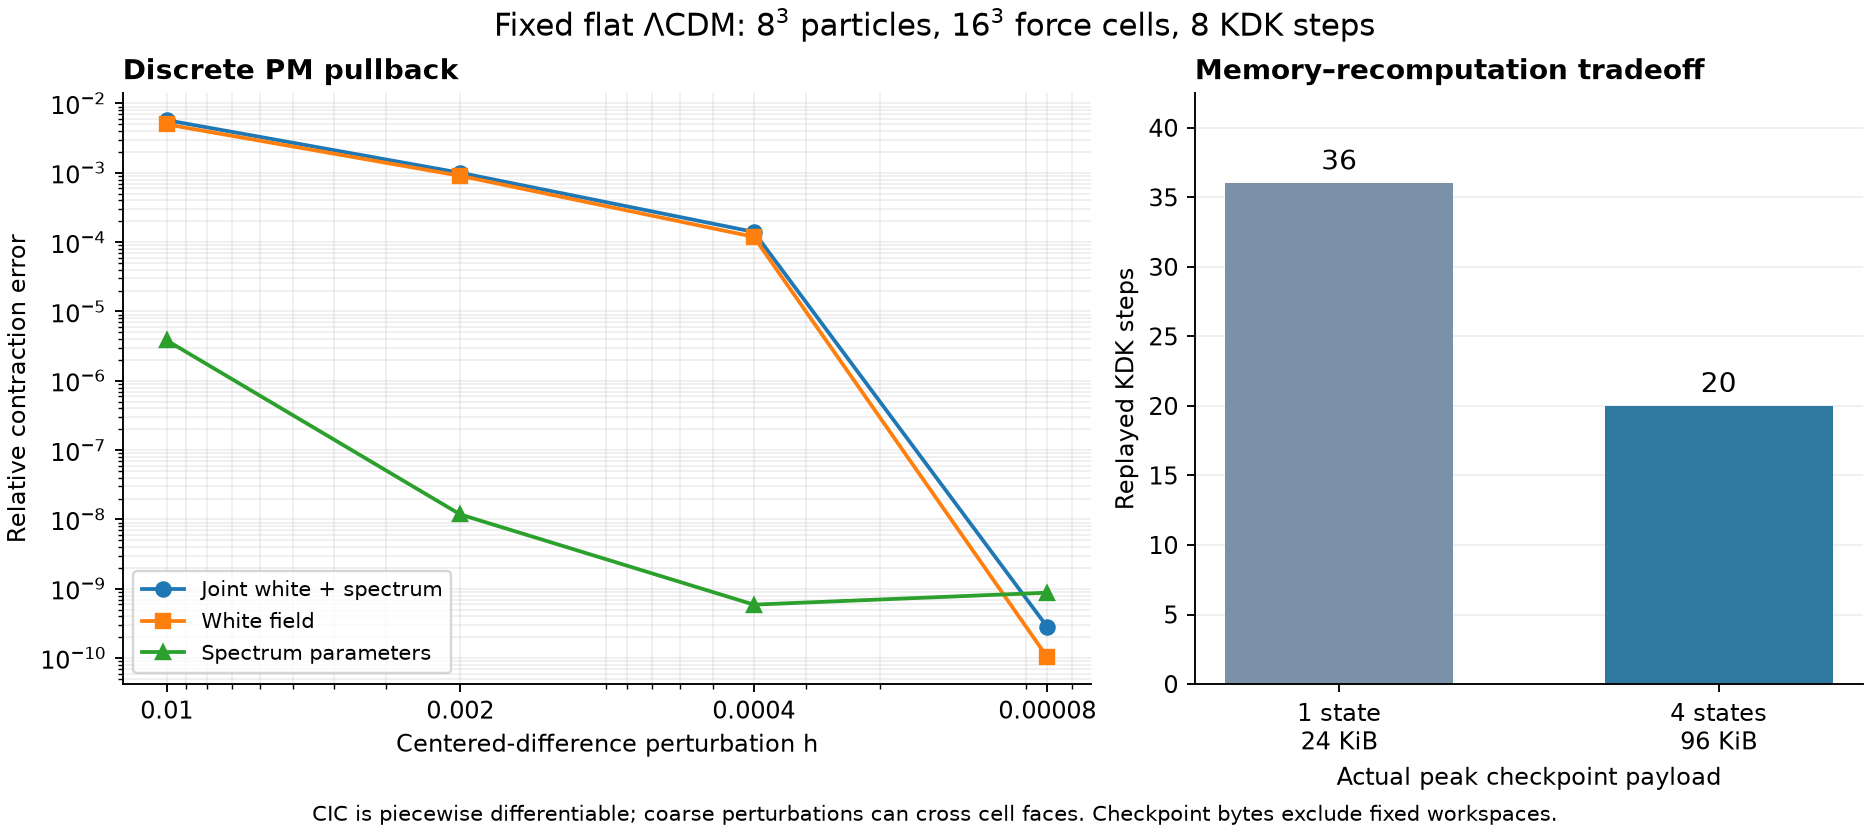
\includegraphics[width=0.9\textwidth]{fieldlevel_pm_adjoint}
\caption{The discrete adjoint of the particle-mesh forward model ($8^3$ particles, $16^3$ force cells, 8 kick-drift-kick steps): the relative
error of the reverse-mode contraction against centred finite differences as the step $h$ decreases, and the number of replayed steps for
one or four stored states (\file{FieldLevel/tests/figures}).}
\label{fig:fl-pm-adjoint}
\end{figure}


\section{Inference}\label{sec:fl-inference}

For linear evolution at fixed parameters the posterior of the field is Gaussian: \code{linear_conditional} gives the exact mean, the Fourier covariance and the
field-marginalised likelihood, used as references. \code{map} finds the maximum a posteriori field (and optionally parameters) with a Fourier preconditioner and
line search. \code{sample} uses the Hamiltonian Monte Carlo of \cref{ch:sampling-fitting} \cite{Duane1987,Neal2011} with a Fourier-diagonal mass for the field (the
linear Hessian $1+b^2P/P_\epsilon$, frozen at the initial parameters), adapted masses for the scalars, and a callback to stream field samples (initial and matter
densities, displacements, velocities). Partial centring of the field, $s_k=(T(\theta_{\rm ref})/T(\theta))^cx_k$ with $c=S/(S+N)$ per mode, decorrelates the field and
the spectrum parameters (the BAO autocorrelation time drops from $\sim13$ to $\sim3$).

\paragraph*{Distribution and restart.} The distributed backends run the linear, 1LPT and 2LPT models, their adjoints, exact conditionals, MAP and HMC over MPI on slab
or pencil grids, with particle/mesh communication for the assignment (\cref{ch:mass-assignment}); checkpoints save the complete HMC and adaptation state with an identity
fingerprint of the backend and grid partition for exact same-layout restarts.

\paragraph*{Surveys.} \file{SurveyLikelihood.h} adds a masked Cartesian observation on the initial mesh: a window with observed flags and selection per cell, the model's
Fourier modes synthesised to real space, and either a Gaussian field likelihood or a Poisson count likelihood with a positive log-link,
$\ln\lambda_i=\ln E_i+\ln S_i+\delta_i-{\rm offset}$, $U_i=\lambda_i-n_i\ln\lambda_i+\ln n_i!$, both with MPI adjoints.

\section{BAO application}\label{sec:fl-bao}

\file{FieldLevelBAO.h} is a prototype of field-level BAO inference \cite{Babic2024}: the BAO scale $\beta=r_{\rm BAO}/r_{\rm fid}$ is sampled with the initial field, the
spectrum being a no-wiggle Eisenstein--Hu shape times $1+A\sin(k\beta r_{\rm fid}+\phi)e^{-k/k_d}$, with linear, 1LPT and 2LPT+bias+RSD forward models (bias, growth
rate and noise fixed). For the linear model the marginal posterior of $\beta$ is known exactly and HMC agrees with it ($1.0232\pm0.0333$ exact, $1.0221\pm0.0330$ HMC on
$32^3$, $k_{\max}=0.095\hMpc$).

\begin{figure}[htbp]
\centering
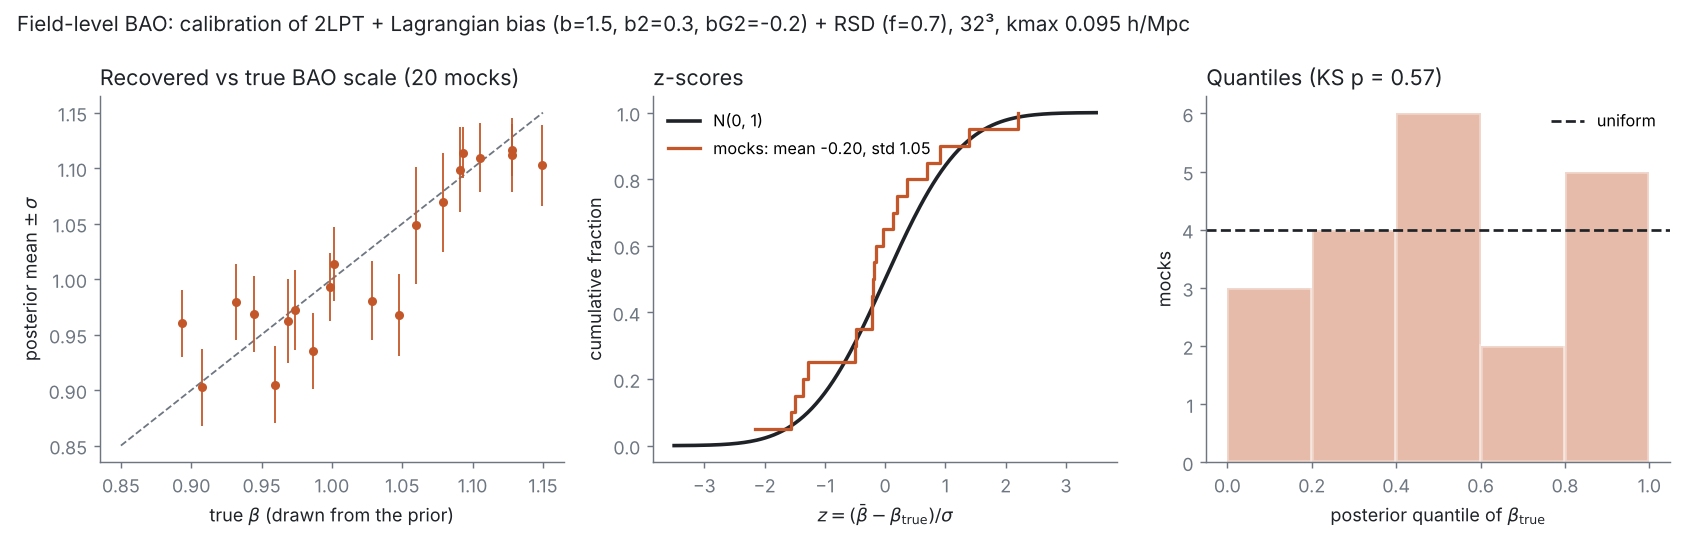
\includegraphics[width=\textwidth]{fieldlevel_bao_calibration}
\caption{Simulation-based calibration of field-level BAO inference with 2LPT, Lagrangian bias ($b=1.5$, $b_2=0.3$, $b_{\mathcal G_2}=-0.2$) and
RSD ($f=0.7$) on $32^3$, $k_{\max}=0.095\hMpc$ (20 mocks, $\beta_{\rm true}$ drawn from the prior): the recovered scale, the $z$-scores against
$\mathcal N(0,1)$ and the posterior quantiles of the true value (\file{FieldLevel/docs/images/calibration.png}).}
\label{fig:fl-calibration}
\end{figure}


\begin{validation}[Validation: field level]
Adjoint gradients against finite differences for all models (relative $\sim10^{-8}$); 2LPT of two orthogonal plane waves against the analytic displacement to $10^{-16}$;
the 2LPT+bias+RSD prediction equals $(b+f\mu^2)\delta_L$ in the linear regime to 0.3\%; mock $\chi^2$ equal to the number of modes. Simulation-based calibration
\cite{Talts2018}: for linear, 1LPT and the full 2LPT+bias+RSD model (20--30 mocks each) $z=(\bar\beta-\beta_{\rm true})/\sigma$ has mean consistent with zero and unit width and
the posterior quantiles are uniform (KS $p=0.57$--0.85). The distributed backends agree with the serial ones for any decomposition; the survey layer is validated with
dispersed 2LPT chains against exact active-mode and masked linear-Gaussian references (\file{FieldLevel/validation/survey}). These checks establish the numerics and sampler, not
nonlinear accuracy against simulations or a production survey analysis.
\end{validation}

\chapter{Sampling, optimisation and cosmology fitting}\label{ch:sampling-fitting}
\chapterstatus{written}{2026-11-19}

General samplers and optimisers for any posterior (adaptive Metropolis--Hastings, Hamiltonian Monte Carlo, Nelder--Mead with profile
likelihoods), convergence diagnostics, and the program \file{./mcmc} that fits cosmological parameters to supernova, BAO and CMB data with
the Einstein--Boltzmann solver as the theory.

\begin{modulebox}{MCMC, CosmologyFitting}
\nsp{FML::MCMC}: \file{MCMC/Posterior.h} (\cls{Posterior}, \cls{SampledParameter}), \file{MCMC/Sampler.h} (\cls{Sampler}), \file{MCMC/Minimizer.h}
(\cls{Minimizer}), \file{MCMC/HMC.h} (\code{run_hmc}, \cls{HMCOptions}, \cls{HMCMass}), \file{MCMC/HMCCheckpoint.h}, \file{MCMC/Diagnostics.h}
(\code{diagnose_chains}), \file{MCMC/Parallel.h}. \nsp{FML::COSMOLOGY::FITTING}: \file{CosmologyFitting/Theory.h}, \file{Likelihoods.h},
\file{SampledParameterMap.h}; the program \file{CosmologyFitting/mcmc} with parameter files in \file{params/} and data in \file{external/}.\par
Documentation: \file{MCMC/README.md}, \file{CosmologyFitting/README.md}. Tests: \file{MCMC/tests}, \file{CosmologyFitting/tests}.
\end{modulebox}

\section{Metropolis--Hastings}\label{sec:fit-mh}

\cls{Sampler} runs several chains in parallel (OpenMP threads and MPI processes) for a \cls{Posterior}: sampled parameters with flat priors, optional
Gaussian priors and a proposal step, derived parameters, and a likelihood function. During burn-in the proposal covariance and scale adapt towards 25\%
acceptance \cite{Haario2001}; at the end of burn-in the covariance pooled from all chains is frozen, so the sampling phase is an exact Markov chain. Points
where the likelihood throws or is not finite are rejected. Fast parameters (e.g.\ likelihood nuisances, for which the theory is cached) get extra updates along
their conditional covariance \cite{Lewis2013}. The run stops when every chain has enough samples and the multivariate Gelman--Rubin $R-1$ (the largest eigenvalue
of $W^{-1}B$, as CosmoMC and Cobaya \cite{Gelman1992}) is below the threshold. Checkpoints hold the complete chain state, so a resumed run continues exactly as
an uninterrupted one, with any number of processes. Output is in GetDist format.

\section{Hamiltonian Monte Carlo}\label{sec:fit-hmc}

\file{HMC.h} samples a potential $U=-\ln p$ with its gradient \cite{Duane1987,Neal2011}, for problems with many parameters such as field-level inference
(\cref{ch:field-level}). The state is a custom block (e.g.\ a field) with a mass given as operators ($M^{1/2}$ on white noise and $M^{-1}$; nothing of it is
recorded) followed by parameters with a diagonal mass adapted in Stan's windows. Leapfrog with a jittered number of steps; the step size is adapted by dual
averaging \cite{HoffmanGelman2014} to a target acceptance; bounds are handled by reflection; divergences are counted. \cls{HMCState} holds the complete state
(including the random generator and adaptation) for exact continuation, with a versioned, checksummed binary codec.

\section{Optimisation and profiles}\label{sec:fit-minimizer}

\cls{Minimizer} maximises the posterior with the Nelder--Mead simplex with adaptive coefficients \cite{GaoHan2012} in coordinates whitened by a covariance,
restarting around the best point until a restart gains less than a tolerance, from several starts in parallel; with fast parameters an inner simplex minimises
them at each slow point. \code{profile} gives profile likelihoods (independent of priors and volume effects) and \code{hessian} the covariance from central
differences with adapted steps.

\section{Diagnostics}\label{sec:fit-diagnostics}

\file{Diagnostics.h} implements the rank-normalised split-$\hat R$, its folded version, and bulk and tail effective sample sizes \cite{Vehtari2021}: ranks with
average ties and Blom scores $(r-3/8)/(S+1/4)$, multi-chain variance, FFT autocovariances and Geyer's initial positive/monotone sequence; the tail ESS is the
minimum of the 5\% and 95\% quantile-indicator ESS. Degenerate cases (too few chains or draws, frozen chains, non-finite values) are reported as statuses rather
than numbers. $\hat R<1.01$ and ESS above $\sim100$ per chain are screening criteria, not guarantees.

\begin{validation}[Validation: samplers]
Sampler: correlated Gaussians, priors, rejected regions, GetDist output, fast/slow and checkpoint/resume. HMC: diagonal mass adaptation over six decades of
variance, an operator mass block coupled to parameters, reflection at bounds. Minimiser: a 4D Gaussian with a prior (maximum to $<0.005\sigma$), Rosenbrock
($2\times10^{-5}$), a maximum on a prior boundary, two peaks, fast/slow, exact profile and Hessian covariance. Diagnostics: fixtures from ArviZ 0.21.0.
\end{validation}

\section{Cosmology fitting}\label{sec:fit-cosmology}

\file{./mcmc} reads a parameter file in the format of the solver's \file{./cmb} (\cref{ch:background}): any solver parameter can be fixed, \code{sample_<name> =
start, min, max, step} samples it (also the aliases \code{H0}, \code{omega_b}, \code{omega_cdm}, \code{Omega_m}, \code{logA}, \code{tau_reio} and
\code{theta_MC_100}), and \code{sampler} selects \code{mcmc}, \code{minimize} (with profiles and a Hessian) or \code{hessian}. The theory is computed only as far as
the likelihoods need: the background for supernovae; the recombination history for BAO and distance priors ($r_d$, $z_*$); the full lensed CMB spectra for the
CMB likelihoods. The likelihoods:
\begin{itemize}
\item supernovae: Pantheon+ \cite{Brout2022}, DES-SN5YR \cite{DESY5}, DES-Dovekie \cite{Popovic2025} and Union3 \cite{Rubin2023}, with the absolute magnitude
      marginalised analytically;
\item BAO: DESI DR1 and DR2 with full covariance \cite{DESI2025}; BBN $\omega_b$;
\item DESI DR1 full shape \cite{DESI2024VII}: the rotated $P_0$, $P_2$ of the six samples with their window and systematics, as DESI's own likelihood: velocileptors'
      REPT with the loops of the linear $P_{cb}$ at the first redshift scaled by $D^4$, the linear terms and $f(k)=(P_{\theta\theta}/P_{cb})^{1/2}$ at each redshift
      (\cref{ch:perturbation-theory}), the peak-average no-wiggle filter, AP, the physical bias basis and the counterterms and stochastic terms marginalised analytically;
\item CMB: Planck 2018 distance priors \cite{Chen2019DP}, plik\_lite TTTEEE/TT with the low-$\ell$ TT compressed \cite{Planck2018spectra,PrinceDunkley2019}, the Planck 2018
      lensing likelihood \cite{Planck2018lensing} (also CMB-marginalised), Planck 2018's low-$\ell$ TT (Commander) and EE (SimAll) likelihoods
      \cite{Planck2018spectra} and the high-$\ell$ CamSpec PR4 (NPIPE) TTTEEE likelihood \cite{Rosenberg2022} with its foreground residuals and calibrations (ported from
      Cobaya), the ACT DR6 (+ Planck PR4) lensing likelihood \cite{Madhavacheril2023,Qu2023} with its CMB-dependent normalisation and $N_1$ corrections
      (linear in the spectra, precomputed as matrices on the bandpowers), and an exact mock Gaussian likelihood of TT, TE, EE (and BB) for forecasts and tests.
\end{itemize}
With several likelihoods each $\chi^2$ is a derived parameter, as are $H_0$, $\Om$, the age, $r_d$, $\theta_*$, $\sigma_8$ and $S_8$.

\paragraph*{The Fading Dark Sector.} \file{params/mcmc_fds_cmb_desi_dovekie.ini} and \file{mcmc_fds_cmb_desi15_dovekie.ini} are the fits
of Obied, Vafa \& Wu \cite{ObiedVafaWu2026} (\code{model = fading_dark_sector}, $c$ and $c'\ge0$ sampled): CamSpec PR4, the Planck low-$\ell$ TT
and EE, ACT DR6 + Planck PR4 lensing, DESI DR2 BAO and DES-Dovekie, with the DESI DR1 full shape in the second. The nonlinear lensing and shear
spectra can use \code{nonlinear = react}, which supports the coupled dark matter (\cref{sec:hm-react}). The full shape uses EdS loop kernels
with the model's linear $P_{cb}$, $P_{\theta\theta}$ and growth, whereas the paper uses exact-time two-fluid kernels (CDM with the fifth force
and the drag, baryons without). \file{tests/check_fds_kernels} computes both for the same linear $P_{cb}$: at $c=-0.85$, $c'=0.053$,
$z=0.3$--1.5 and $k\le0.2\hMpc$ the exact-time $\delta\delta$ loop differs from EdS by $\le3\times10^{-3}$ of $P_L$ and the $\theta\theta$
loop by $\le1\%$ of $f^2P_L$, almost all of it present in $\Lambda$CDM as well; the part due to the fifth force and the drag is
$\le4\times10^{-4}$ and $3\times10^{-3}$. Mapped onto the DESI multipoles (\file{python/fds_kernels_dchi2.py}) the whole difference
changes $\chi^2$ by 0.011 (0.001 after refitting $b_1$, $\alpha_0$, $\alpha_2$ and the shot noise) and the FDS-specific part by 0.001,
against the model's $\Delta\chi^2\approx-14$ to $-20$: EdS kernels are enough for these fits.

\begin{paramfile}[A w0wa fit to DESI DR2, Planck distance priors and Pantheon+]
model       = w0wa
likelihoods = desi_dr2, planck_dp, pantheonplus
sample_H0      = 68, 50, 90, 0.5, H_0
sample_omega_b = 0.0224, 0.019, 0.026, 0.0002, \omega_b
sample_Omega_m = 0.31, 0.2, 0.4, 0.005, \Omega_m
sample_w0      = -0.9, -2, 0, 0.05, w_0
sample_wa      = -0.5, -3, 2, 0.2, w_a
mcmc_chains = 4
mcmc_output = chains/w0wa
\end{paramfile}

\begin{validation}[Validation: cosmology fitting]
Distances against independent integrals, $r_d$ against CLASS to $10^{-4}$, the distance priors at the Planck best fit within $0.3\sigma$; plik\_lite equal to planck-lite-py
to $10^{-13}$ in $\ln L$ and the lensing likelihood equal to Cobaya's to $10^{-14}$; supernova likelihoods equal to an independent Python implementation to $10^{-5}$ in
$\chi^2$; the Planck low-$\ell$ TT and EE likelihoods equal to Cobaya's to $10^{-14}$ in $\ln L$ and CamSpec PR4 to $10^{-8}$ (relative) in $\chi^2$, ACT DR6 lensing equal to act\_dr6\_lenslike to $10^{-14}$; DESI DR1 full shape equal to DESI's code path (velocileptors) to $10^{-7}$ in $\ln L$ for the same
linear inputs, whose $P_{cb}$ agrees with CAMB's to $10^{-4}$. DESI DR2 + BBN gives $\Om=0.2975\pm0.0085$, $hr_d=101.53\pm0.72$\,Mpc, $H_0=68.53\pm0.60$, as the DESI analysis. DESI DR2 + distance priors + Pantheon+ in $w_0w_a$:
$w_0=-0.848\pm0.054$, $w_a=-0.55\pm0.22$, $\Delta\chi^2=-7.6$ against $\Lambda$CDM. The plik\_lite (+ lensing) best fit agrees with the Planck 2018 best-fit parameters to a
fraction of $\sigma$; mock CMB fits with isocurvature, tensors or ultralight axions recover the fiducial values.
\end{validation}

\begin{figure}[htbp]
\centering
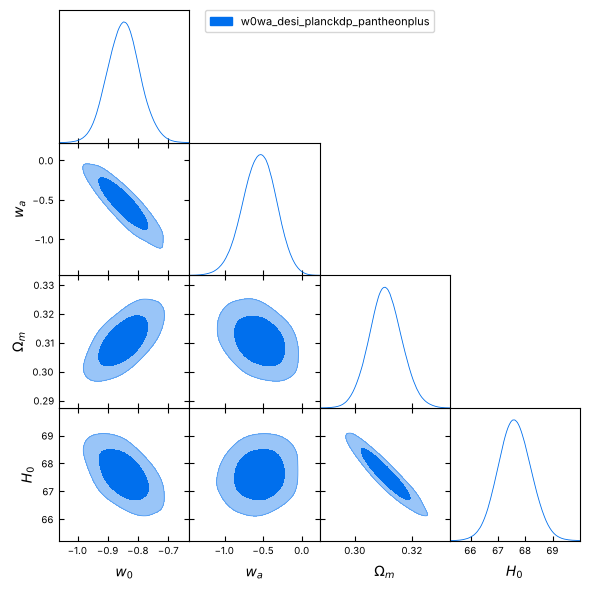
\includegraphics[width=0.6\textwidth]{fitting_w0wa}
\caption{Marginalised posteriors of $w_0$, $w_a$, $\Om$ and $H_0$ from DESI DR2 BAO, the Planck 2018 distance priors and Pantheon+ with
\file{./mcmc} (\file{params/mcmc_w0wa.ini}; 68\% and 95\% contours).}
\label{fig:fit-w0wa}
\end{figure}



\part{Applications}
\chapter{Snapshot analysis}\label{ch:snapshot-analyzer}
\chapterstatus{written}{2026-11-15}

The analyses of the previous chapters are collected in an analysis layer that takes N-body particles and a description of the
cosmology and units, independent of any simulation code or file format. The standalone program \file{SnapshotAnalyzer} uses it to
post-process GADGET snapshots of any code with the same parameters, algorithms and output files as \file{SimulationCode}.

\begin{modulebox}{Analysis, SnapshotAnalyzer}
\nsp{FML::ANALYSIS}: \file{Analysis/AnalysisContext.h} (\cls{AnalysisContext}, \cls{Background}), \file{DensityGrid.h}, \file{PowerSpectrum.h},
\file{HybridBias.h}, \file{CosmicWeb.h}, \file{Minkowski.h}, \file{Halos.h}, \file{Baryonification.h}, \file{Voids.h}, \file{DTFE.h},
\file{ParticleUtils.h}, \file{Output.h}; the program \file{SnapshotAnalyzer/src/Main.cpp}, \file{SnapshotAnalyzer.h}.\par
Documentation: \file{Analysis/README.md}, \file{SnapshotAnalyzer/README.md}. Tests: \file{Analysis/tests}, \file{SnapshotAnalyzer/tests}.
\end{modulebox}

\section{The analysis layer}\label{sec:sa-layer}

An analysis receives the particles (positions in $[0,1)$) and an \cls{AnalysisContext}: the box size, the scale factor, the expansion history
(\code{Background::LCDM}, a table of $H/H_0$, or any function $E(a)$, with $\Omega_{m0}$) and the conversions of the particle mass and velocity units to
$M_\odot/h$ and peculiar km/s. From these follow the redshift-space displacement factor $v_{\rm unit}/(100aE(a)B)$ and the density parameter of the
particles (so \code{200c} masses are right whatever the particles represent, e.g.\ CDM and baryons only). Each analysis has a settings struct with the same
keys and defaults as \file{SimulationCode}, described once by a \code{parameters(f)} visitor so that any parameter reader can fill it. All functions are
collective, and an error on one task becomes an exception on every task.

\begin{table}[ht]
\centering\small
\caption{The analyses of the analysis layer, with their chapters and output files.}
\label{tab:analyses}
\begin{tabularx}{\textwidth}{@{}lXl@{}}
\toprule
Analysis & Method & Output \\
\midrule
\code{measure_power_spectrum} & $P(k)$ (\cref{sec:pk-estimator}) & \file{pofk_z<z>.txt} \\
\code{measure_power_spectrum_multipoles} & $P_\ell(k)$ in redshift space (\cref{sec:pk-multipoles}) & \file{pofk_multipole_z<z>.txt} \\
\code{measure_bispectrum} & $B(k_1,k_2,k_3)$ and $Q$ (\cref{sec:pk-polyspectra}) & \file{bispectrum_z<z>.txt} \\
\code{measure_hybrid_bias} & hybrid bias spectra (\cref{sec:pk-hybrid}) and multipoles (\cref{sec:pk-hybrid-rsd}) & \file{hybridbias_[rsd_]z<z>.txt} \\
\code{measure_cosmic_web} & T-web fractions (\cref{sec:web-tweb}) & \file{cosmicweb_z<z>.txt} \\
\code{measure_minkowski_functionals} & $V_0$--$V_3$ and Gaussian predictions (\cref{sec:web-minkowski}) & \file{minkowski_z<z>.txt} \\
\code{find_halos} & FoF/relaxed FoF, SO masses, overlaps (\cref{ch:halo-finding}) & \file{halos_z<z>.txt}, \file{massfunc_*} \\
\code{find_*_voids} & voxel, spherical, ZOBOV voids (\cref{sec:voids-finders}) & \file{voids_*z<z>.txt} \\
\code{compute_dtfe_fields} & DTFE density and velocity fields and spectra (\cref{sec:voids-dtfe}) & \file{dtfe_spectra_z<z>.txt} \\
\code{baryonify} & position-only baryonification (\cref{ch:pgd-baryonification}) & \file{baryonification_z<z>.txt} \\
\code{project_image} & images of a slab of the density and of $-\nabla\cdot\bm v/(aH)$ (\file{Images.h},
\cref{sec:io-visualization}) & \file{image_<field>_z<z>.png} \\
\bottomrule
\end{tabularx}
\end{table}

For the hybrid bias spectra the linear field comes from an initial-conditions snapshot of the same particles (the lattice and $\delta_L=-\nabla\cdot\bm\Psi$ of the
displacements, matched by ID, with the second-order part removed for 2LPT initial conditions) or from the file written by \file{SimulationCode}, and is scaled by
$D(z)/D(z_L)$ of the analysis cosmology. With \param{hybridbias_rsd} the operators are also assigned at the redshift-space
positions (the velocities converted as for the multipoles) and the multipoles up to \param{hybridbias_rsd_ellmax} written.

\section{SnapshotAnalyzer}\label{sec:sa-program}

\file{SnapshotAnalyzer} reads GADGET binary or HDF5 snapshots (\cref{sec:io-snapshots}): each task reads every $N_{\rm tasks}$-th file and the particles are sent to
their owners, optionally selecting particle types. The cosmology is $\Lambda$CDM from the header (plus radiation) or a table of $H/H_0$ (e.g.\ the one written by
\file{SimulationCode}). It runs any of the analyses of \cref{tab:analyses} from a Lua parameter file with \file{SimulationCode}'s parameter names; unknown names give a
warning and names of earlier versions an error with the replacement. ZOBOV and the DTFE need CGAL, HDF5 snapshots \code{USE_HDF5}.

\begin{paramfile}[A SnapshotAnalyzer parameter file]
snapshot_input  = "./output/gadget_z0.000"
snapshot_format = "gadget"
output_folder   = "./analysis"
pofk = true
pofk_nmesh = 256
pofk_density_assignment_method = "PCS"
pofk_interlacing = true
fof = true
fof_linking_length = 0.2
fof_so_definitions = {"200m", "500c", "vir"}
cosmicweb = true
cosmicweb_smoothing_scale_mpch = 2.0
\end{paramfile}

\begin{validation}[Validation: analysis]
\file{Analysis/tests} on 1, 2 and 4 tasks: units and SO thresholds, FoF/SO/overlaps on particles with known halos, mass functions, particle redistribution, baryonification
(particles conserved, hosts, $P(k)$ unchanged on large scales), voids around a spherical hole, ZOBOV and DTFE velocity units, the growth ratio, exact hybrid-bias fields of a
Zel'dovich lattice and ID matching, T-web fractions $(0.08,0.42,0.42,0.08)$ at $\lambda_{\rm th}=0$ for a Gaussian field. On a \file{SimulationCode} snapshot the bispectrum equals the
in-run one to the float32 precision of the positions ($\sim2\times10^{-6}$) and the hybrid bias spectra from the linear-field file equal the in-run ones to $2\times10^{-5}$.
\end{validation}


\appendix
\chapter{Module index}\label{app:module-index}
\chapterstatus{written}{2026-11-15}

Every module directory of \file{FML/} and the chapters that describe it. Directories not listed (\file{tests},
build and output folders) contain no library code.

\begin{longtable}{@{}ll@{}}
\toprule
Module & Described in \\
\midrule
\endfirsthead
\toprule
Module & Described in \\
\midrule
\endhead
\file{AMRCode} & \cref{sec:sr-amr} \\
\file{AdaptiveMPIGrid} & \cref{ch:grids-fft,ch:multigrid} \\
\file{Analysis} & \cref{ch:snapshot-analyzer} \\
\file{AxionHMcode} & \cref{ch:halo-model} \\
\file{Baryonification} & \cref{ch:pgd-baryonification} \\
\file{Chunkpix} & \cref{ch:io-utilities} \\
\file{ComputePowerSpectra} & \cref{ch:power-spectra} \\
\file{ConnectedFourPoint} & \cref{ch:ensembles} \\
\file{CosmicWeb} & \cref{ch:cosmic-web} \\
\file{Cosmology/Background} & \cref{ch:background} \\
\file{Cosmology/EinsteinBoltzmannSolver} & \cref{ch:background,ch:cmb-spectra} \\
\file{Cosmology/Growth} & \cref{ch:growth-transfer} \\
\file{Cosmology/Perturbations} & \cref{ch:linear-perturbations,ch:extended-models} \\
\file{Cosmology/Recombination} & \cref{ch:recombination} \\
\file{Cosmology/Spectra} & \cref{ch:cmb-spectra,ch:fitting-emulators} \\
\file{CosmologyFitting} & \cref{ch:sampling-fitting} \\
\file{CountsInCells} & \cref{ch:configuration-space} \\
\file{Emulator} & \cref{ch:fitting-emulators} \\
\file{ExampleData} & \cref{ch:io-utilities} \\
\file{EnsembleStatistics} & \cref{ch:ensembles} \\
\file{Environment} & \cref{ch:configuration-space} \\
\file{FFTLog} & \cref{ch:numerics} \\
\file{FFTWGrid} & \cref{ch:grids-fft} \\
\file{FieldLevel} & \cref{ch:field-level} \\
\file{FileUtils} & \cref{ch:io-utilities} \\
\file{FriendsOfFriends} & \cref{ch:halo-finding} \\
\file{GadgetUtils} & \cref{ch:io-utilities} \\
\file{GlassIC} & \cref{ch:lpt} \\
\file{Global} & \cref{ch:parallelism} \\
\file{HOD} & \cref{ch:galaxy-mocks} \\
\file{HaloHistory} & \cref{ch:halo-finding} \\
\file{HaloModel} & \cref{ch:halo-model} \\
\file{Hydrodynamics} & \cref{ch:hydro-wavedm} \\
\file{InitialConditions} & \cref{ch:growth-transfer} \\
\file{Interpolation} & \cref{ch:mass-assignment} \\
\file{KDTree} & \cref{ch:particles} \\
\file{LPT} & \cref{ch:lpt} \\
\file{LatinHyperCube} & \cref{ch:numerics} \\
\file{LuaFileParser} & \cref{ch:io-utilities} \\
\file{MCMC} & \cref{ch:sampling-fitting} \\
\file{MPIGrid} & \cref{ch:grids-fft} \\
\file{MPIParticles} & \cref{ch:particles} \\
\file{MakePythonWrapper} & \cref{ch:io-utilities} \\
\file{Math} & \cref{ch:numerics} \\
\file{MemoryLogging} & \cref{ch:io-utilities} \\
\file{Morphology} & \cref{ch:cosmic-web} \\
\file{MultigridSolver} & \cref{ch:multigrid} \\
\file{NBody} & \cref{ch:nbody-pm} \\
\file{NUFFT} & \cref{ch:mass-assignment} \\
\file{ODESolver} & \cref{ch:numerics} \\
\file{PGD} & \cref{ch:pgd-baryonification} \\
\file{PairCounting} & \cref{ch:configuration-space} \\
\file{ParameterMap} & \cref{ch:io-utilities} \\
\file{ParticleTypes} & \cref{ch:particles} \\
\file{ParticlesInBoxes} & \cref{ch:particles} \\
\file{PeanoHilbertDomain} & \cref{ch:parallelism} \\
\file{PencilDomain} & \cref{ch:parallelism} \\
\file{Performance} & \cref{ch:io-utilities} \\
\file{PerturbationTheory} & \cref{ch:perturbation-theory} \\
\file{PhaseSpaceHaloFinder} & \cref{ch:halo-finding} \\
\file{Plotting} & \cref{ch:io-utilities} \\
\file{PythonAnalysis} & \cref{ch:io-utilities} \\
\file{RamsesUtils} & \cref{ch:io-utilities} \\
\file{RandomFields} & \cref{ch:random-fields} \\
\file{RandomGenerator} & \cref{ch:numerics,ch:random-fields} \\
\file{SPH} & \cref{ch:hydro-wavedm} \\
\file{ShortRangeGravity} & \cref{ch:short-range} \\
\file{SimulationCode} & \cref{ch:simulation-code,ch:mg-simulations,ch:nbody-pm} \\
\file{Smoothing} & \cref{ch:mass-assignment} \\
\file{SnapshotAnalyzer} & \cref{ch:snapshot-analyzer} \\
\file{SphericalCollapse} & \cref{ch:spherical-collapse} \\
\file{Spline} & \cref{ch:numerics} \\
\file{Survey} & \cref{ch:surveys} \\
\file{ThreePointCorrelation} & \cref{ch:configuration-space} \\
\file{TidalTensor} & \cref{ch:cosmic-web} \\
\file{Timing} & \cref{ch:io-utilities} \\
\file{TransferProviders} & \cref{ch:growth-transfer} \\
\file{Triangulation} & \cref{ch:voids} \\
\file{Units} & \cref{ch:io-utilities,ch:conventions} \\
\file{Visualization} & \cref{sec:io-visualization} \\
\file{VoidFinders} & \cref{ch:voids} \\
\file{WaveDarkMatter} & \cref{ch:hydro-wavedm} \\
\file{WeakLensing} & \cref{ch:weak-lensing} \\
\bottomrule
\end{longtable}


\backmatter
\bibliographystyle{unsrtnat}
\cleardoublepage
\phantomsection
\addcontentsline{toc}{chapter}{Bibliography}
\bibliography{references}
\cleardoublepage\phantomsection\addcontentsline{toc}{chapter}{\indexname}
\printindex
\end{document}
